% Options for packages loaded elsewhere
\PassOptionsToPackage{unicode}{hyperref}
\PassOptionsToPackage{hyphens}{url}
%
\documentclass[
]{book}
\usepackage{amsmath,amssymb}
\usepackage{iftex}
\ifPDFTeX
  \usepackage[T1]{fontenc}
  \usepackage[utf8]{inputenc}
  \usepackage{textcomp} % provide euro and other symbols
\else % if luatex or xetex
  \usepackage{unicode-math} % this also loads fontspec
  \defaultfontfeatures{Scale=MatchLowercase}
  \defaultfontfeatures[\rmfamily]{Ligatures=TeX,Scale=1}
\fi
\usepackage{lmodern}
\ifPDFTeX\else
  % xetex/luatex font selection
\fi
% Use upquote if available, for straight quotes in verbatim environments
\IfFileExists{upquote.sty}{\usepackage{upquote}}{}
\IfFileExists{microtype.sty}{% use microtype if available
  \usepackage[]{microtype}
  \UseMicrotypeSet[protrusion]{basicmath} % disable protrusion for tt fonts
}{}
\makeatletter
\@ifundefined{KOMAClassName}{% if non-KOMA class
  \IfFileExists{parskip.sty}{%
    \usepackage{parskip}
  }{% else
    \setlength{\parindent}{0pt}
    \setlength{\parskip}{6pt plus 2pt minus 1pt}}
}{% if KOMA class
  \KOMAoptions{parskip=half}}
\makeatother
\usepackage{xcolor}
\usepackage{color}
\usepackage{fancyvrb}
\newcommand{\VerbBar}{|}
\newcommand{\VERB}{\Verb[commandchars=\\\{\}]}
\DefineVerbatimEnvironment{Highlighting}{Verbatim}{commandchars=\\\{\}}
% Add ',fontsize=\small' for more characters per line
\usepackage{framed}
\definecolor{shadecolor}{RGB}{248,248,248}
\newenvironment{Shaded}{\begin{snugshade}}{\end{snugshade}}
\newcommand{\AlertTok}[1]{\textcolor[rgb]{0.94,0.16,0.16}{#1}}
\newcommand{\AnnotationTok}[1]{\textcolor[rgb]{0.56,0.35,0.01}{\textbf{\textit{#1}}}}
\newcommand{\AttributeTok}[1]{\textcolor[rgb]{0.13,0.29,0.53}{#1}}
\newcommand{\BaseNTok}[1]{\textcolor[rgb]{0.00,0.00,0.81}{#1}}
\newcommand{\BuiltInTok}[1]{#1}
\newcommand{\CharTok}[1]{\textcolor[rgb]{0.31,0.60,0.02}{#1}}
\newcommand{\CommentTok}[1]{\textcolor[rgb]{0.56,0.35,0.01}{\textit{#1}}}
\newcommand{\CommentVarTok}[1]{\textcolor[rgb]{0.56,0.35,0.01}{\textbf{\textit{#1}}}}
\newcommand{\ConstantTok}[1]{\textcolor[rgb]{0.56,0.35,0.01}{#1}}
\newcommand{\ControlFlowTok}[1]{\textcolor[rgb]{0.13,0.29,0.53}{\textbf{#1}}}
\newcommand{\DataTypeTok}[1]{\textcolor[rgb]{0.13,0.29,0.53}{#1}}
\newcommand{\DecValTok}[1]{\textcolor[rgb]{0.00,0.00,0.81}{#1}}
\newcommand{\DocumentationTok}[1]{\textcolor[rgb]{0.56,0.35,0.01}{\textbf{\textit{#1}}}}
\newcommand{\ErrorTok}[1]{\textcolor[rgb]{0.64,0.00,0.00}{\textbf{#1}}}
\newcommand{\ExtensionTok}[1]{#1}
\newcommand{\FloatTok}[1]{\textcolor[rgb]{0.00,0.00,0.81}{#1}}
\newcommand{\FunctionTok}[1]{\textcolor[rgb]{0.13,0.29,0.53}{\textbf{#1}}}
\newcommand{\ImportTok}[1]{#1}
\newcommand{\InformationTok}[1]{\textcolor[rgb]{0.56,0.35,0.01}{\textbf{\textit{#1}}}}
\newcommand{\KeywordTok}[1]{\textcolor[rgb]{0.13,0.29,0.53}{\textbf{#1}}}
\newcommand{\NormalTok}[1]{#1}
\newcommand{\OperatorTok}[1]{\textcolor[rgb]{0.81,0.36,0.00}{\textbf{#1}}}
\newcommand{\OtherTok}[1]{\textcolor[rgb]{0.56,0.35,0.01}{#1}}
\newcommand{\PreprocessorTok}[1]{\textcolor[rgb]{0.56,0.35,0.01}{\textit{#1}}}
\newcommand{\RegionMarkerTok}[1]{#1}
\newcommand{\SpecialCharTok}[1]{\textcolor[rgb]{0.81,0.36,0.00}{\textbf{#1}}}
\newcommand{\SpecialStringTok}[1]{\textcolor[rgb]{0.31,0.60,0.02}{#1}}
\newcommand{\StringTok}[1]{\textcolor[rgb]{0.31,0.60,0.02}{#1}}
\newcommand{\VariableTok}[1]{\textcolor[rgb]{0.00,0.00,0.00}{#1}}
\newcommand{\VerbatimStringTok}[1]{\textcolor[rgb]{0.31,0.60,0.02}{#1}}
\newcommand{\WarningTok}[1]{\textcolor[rgb]{0.56,0.35,0.01}{\textbf{\textit{#1}}}}
\usepackage{longtable,booktabs,array}
\usepackage{calc} % for calculating minipage widths
% Correct order of tables after \paragraph or \subparagraph
\usepackage{etoolbox}
\makeatletter
\patchcmd\longtable{\par}{\if@noskipsec\mbox{}\fi\par}{}{}
\makeatother
% Allow footnotes in longtable head/foot
\IfFileExists{footnotehyper.sty}{\usepackage{footnotehyper}}{\usepackage{footnote}}
\makesavenoteenv{longtable}
\usepackage{graphicx}
\makeatletter
\def\maxwidth{\ifdim\Gin@nat@width>\linewidth\linewidth\else\Gin@nat@width\fi}
\def\maxheight{\ifdim\Gin@nat@height>\textheight\textheight\else\Gin@nat@height\fi}
\makeatother
% Scale images if necessary, so that they will not overflow the page
% margins by default, and it is still possible to overwrite the defaults
% using explicit options in \includegraphics[width, height, ...]{}
\setkeys{Gin}{width=\maxwidth,height=\maxheight,keepaspectratio}
% Set default figure placement to htbp
\makeatletter
\def\fps@figure{htbp}
\makeatother
\setlength{\emergencystretch}{3em} % prevent overfull lines
\providecommand{\tightlist}{%
  \setlength{\itemsep}{0pt}\setlength{\parskip}{0pt}}
\setcounter{secnumdepth}{5}
\usepackage{booktabs}
\ifLuaTeX
  \usepackage{selnolig}  % disable illegal ligatures
\fi
\usepackage[]{natbib}
\bibliographystyle{plainnat}
\usepackage{bookmark}
\IfFileExists{xurl.sty}{\usepackage{xurl}}{} % add URL line breaks if available
\urlstyle{same}
\hypersetup{
  pdftitle={Introdução ao R},
  pdfauthor={Renato de Paula},
  hidelinks,
  pdfcreator={LaTeX via pandoc}}

\title{Introdução ao R}
\author{Renato de Paula}
\date{2024-09-03}

\begin{document}
\maketitle

{
\setcounter{tocdepth}{1}
\tableofcontents
}
\chapter{Prefácio}\label{prefuxe1cio}

Este material, ``Introdução ao R'', foi desenvolvido com o objetivo de servir como um guia acessível e prático para os alunos do curso de Laboratório de Estatística I - Introdução à Simulação da Faculdade de Ciências da Universidade de Lisboa. Reconhecendo a importância cada vez maior da análise de dados na ciência moderna, o material aqui apresentado busca introduzir os conceitos fundamentais e as funcionalidades do R, uma ferramenta poderosa e amplamente utilizada na análise estatística.

Ao longo deste material, os leitores serão guiados através de uma série de tópicos essenciais, desde a instalação do software e a navegação no ambiente RStudio, até o manuseio de estruturas de dados complexas e a criação de gráficos sofisticados. Cada capítulo foi estruturado de forma a proporcionar uma compreensão sólida dos conceitos abordados, combinando explicações teóricas com exemplos práticos e exercícios que reforçam o aprendizado.

Este material foi elaborado para atender às necessidades dos alunos, tanto aqueles que estão iniciando seus estudos em Estatística quanto aqueles que já possuem alguma experiência prévia. Acreditamos que, ao concluir este curso, os alunos estarão bem preparados para aplicar técnicas estatísticas em diversas áreas do conhecimento, utilizando o R como uma ferramenta indispensável para suas análises.

\chapter{R e RStudio}\label{r-e-rstudio}

O software de código aberto R foi desenvolvido como uma implementação
livre da linguagem S, que foi projetada como uma linguagem para
computação estatística, programação estatística e gráficos. A intenção
principal era permitir aos usuários explorar os dados de uma forma fácil
e interativa, apoiada em representações gráficas significativas. O
software estatístico R foi originalmente criado por Ross Ihaka e Robert
Gentleman (Universidade de Auckland, Nova Zelândia).

R é um conjunto integrado de recursos de software para manipulação de
dados, cálculo e exibição gráfica. Ele inclui:

\begin{itemize}
\item
  Manuseio eficaz de dados e facilidade de armazenamento;
\item
  Um conjunto de operadores para cálculos em arrays/matrizes;
\item
  Uma coleção grande, coerente e integrada de ferramentas
  intermediárias para análise de dados;
\item
  Recursos gráficos para análise e exibição de dados na tela ou em
  cópia impressa;
\item
  Uma linguagem de programação bem desenvolvida, simples e eficaz que
  inclui condicionais, loops, funções recursivas definidas pelo
  usuário e recursos de entrada e saída.
\end{itemize}

\section{Instalação e funcionalidades básicas}\label{instalauxe7uxe3o-e-funcionalidades-buxe1sicas}

\begin{itemize}
\item
  A versão ``base'' do R, ou seja, o software com seus comandos mais
  relevantes, pode ser baixado em \url{https://www.r-project.org/}. Após
  instalar o R, é recomendável instalar também um editor. Um editor
  permite ao usuário salvar e exibir convenientemente o código R,
  enviar esse código ao R Console e controlar as configurações e a
  saída. Uma escolha popular de editor é o RStudio (gratuito), que
  pode ser baixado em \url{https://www.rstudio.com/}.
\item
  Muitos pacotes adicionais escritos pelo usuário estão disponíveis
  online e podem ser instalados no console R ou usando o menu R.
  Dentro do console, a função
  \texttt{install.packages(“pacote\ para\ instalar”)} pode ser usada. Observe
  que é necessária uma conexão com a Internet.Você pode ver todos os
  pacotes instalados usando a função \texttt{installed.packages()}.
\end{itemize}

\section{Navegando no RStudio}\label{navegando-no-rstudio}

Existem quatro painéis de trabalho no RStudio:

\begin{itemize}
\item
  \textbf{Editor/Scripts}. Este painel é onde os scripts são
  gravados/carregados e exibidos. Possui realce de sintaxe e
  preenchimento automático, além de permitir passar o código linha por
  linha.
\item
  \textbf{Console}. É aqui que os comandos são executados e é
  essencialmente a aparência do console do R básico, só que melhor! O
  console possui realce de sintaxe, preenchimento de código e
  interface com outros painéis do RStudio.
\item
  \textbf{Environment/Histórico}. A aba do espaço de trabalho exibe
  informações que normalmente ficam ocultas no R, como dados
  carregados, funções e outras variáveis. A aba histórico armazena
  todos os comandos (linhas de código) que foram analisados por meio
  do R.
\item
  \textbf{Último painel}. Este painel inclui a aba de arquivos (lista todos
  os arquivos no diretório de trabalho atual), a aba de gráficos
  (quaisquer gráficos), a aba de pacotes (pacotes instalados) e a aba
  de ajuda (sistema de ajuda html embutido).
\end{itemize}

\section{Atalhos}\label{atalhos}

\begin{itemize}
\item
  \textbf{CTRL+ENTER}: compila a(s) linha(s) selecionada(s) no script.
\item
  \textbf{ALT+-}: cria no script um sinal de atribuição (\textless-).
\item
  \textbf{CTRL+SHIFT+M}: (\%\textgreater\%) operador pipe.
\item
  \textbf{CTRL+1}: altera cursor para o script.
\item
  \textbf{CTRL+2}: altera cursor para o console.
\item
  \textbf{CTRL+ALT+I}: cria um chunk no R Markdown.
\item
  \textbf{CTRL+SHIFT+K}: compila um arquivo no R Markdown.
\item
  \textbf{ALT+SHIFT+K}: janela com todos os atalhos disponíveis.
\end{itemize}

No MacBook, os atalhos geralmente são os mesmos, substituindo o \textbf{CTRL}
por \textbf{command} e o \textbf{ALT} por \textbf{option}.

\chapter{R como uma calculadora e Operações Aritméticas}\label{r-como-uma-calculadora-e-operauxe7uxf5es-aritmuxe9ticas}

A estatística tem uma relação estreita com a álgebra: os conjuntos de
dados podem ser vistos como matrizes e as variáveis como vetores. O R
faz uso dessas estruturas e é por isso que primeiro apresentamos
funcionalidades de estrutura de dados antes de explicar alguns dos
comandos estatísticos básicos mais relevantes.

\section{O prompt}\label{o-prompt}

O R possui uma interface de linha de comando e aceitará comandos
simples. Isso é marcado por um símbolo \textgreater, chamado \textbf{prompt}. Se você
digitar um comando e pressionar Enter, o R irá avaliá-lo e imprimir o
resultado para você.

\begin{Shaded}
\begin{Highlighting}[]
\FunctionTok{print}\NormalTok{(}\StringTok{"Meu primeiro comando no R!"}\NormalTok{)}
\DocumentationTok{\#\# [1] "Meu primeiro comando no R!"}
\end{Highlighting}
\end{Shaded}

Observe que nestas notas, caixas cinzas são usadas para mostrar o código
R digitado no console R. O símbolo \#\#{[}1{]} é usado para denotar o output
do console R.

O caractere \texttt{\#} marca o início de um comentário. Todos os caracteres até
o final da linha são ignorados pelo R. Usamos \texttt{\#} para comentar nosso
código R.

\begin{Shaded}
\begin{Highlighting}[]
\CommentTok{\# Meu primeiro comando no R!}
\end{Highlighting}
\end{Shaded}

Se soubermos o nome de um comando que gostaríamos de usar e quisermos
aprender sobre a sua funcionalidade, basta digitar \texttt{?command} no prompt
da linha de comando do R que ele exibe uma página de ajuda. Por exemplo

\begin{Shaded}
\begin{Highlighting}[]
\NormalTok{?sum}
\end{Highlighting}
\end{Shaded}

exibe uma página de ajuda para a função de soma.

\begin{itemize}
\tightlist
\item
  Usando
\end{itemize}

\begin{Shaded}
\begin{Highlighting}[]
\FunctionTok{example}\NormalTok{(sum)}
\end{Highlighting}
\end{Shaded}

mostra exemplos de aplicação da respetiva função.

\section{Objetos e variáveis}\label{objetos-e-variuxe1veis}

Um \textbf{objeto} em R é uma unidade de armazenamento que contém valores ou
funções e pode ser referenciado por um nome. Esses valores podem ser
números, caracteres, vetores, matrizes, data frames, listas, ou até
mesmo funções. Objetos são criados e manipulados através de comandos e
podem ser reutilizados em qualquer parte do código. Tudo o que é criado
ou carregado na sessão de R, como dados ou funções, é considerado um
objeto.

\subsection{O que é uma variável?}\label{o-que-uxe9-uma-variuxe1vel}

Refere-se a um \textbf{nome} ou um identificador que é atribuído a um objeto.
A variável armazena a referência ao objeto em si. Em outras palavras,
uma variável é o nome que você usa para acessar os dados ou a função
armazenada no objeto.

\subsection{Atribuições}\label{atribuiuxe7uxf5es}

\begin{itemize}
\item
  A expressão \texttt{x\textless{}-10} cria uma variável \(x\) e atribui o valor 10 a
  \(x\). Observe que a variável à esquerda é atribuída ao valor à
  direita. O lado esquerdo deve conter apenas um único nome de
  variável.
\item
  Também se pode atribuir usando = (ou \texttt{-\textgreater{}}). Porém, para evitar
  confusão, é comum usar \texttt{\textless{}-} para distinguir do operador de igualdade
  =.
\end{itemize}

\begin{Shaded}
\begin{Highlighting}[]
\CommentTok{\# Atribuição correta }
\NormalTok{a }\OtherTok{\textless{}{-}} \DecValTok{10}
\NormalTok{b }\OtherTok{\textless{}{-}}\NormalTok{ a }\SpecialCharTok{+} \DecValTok{1}
\end{Highlighting}
\end{Shaded}

\begin{Shaded}
\begin{Highlighting}[]
\CommentTok{\# Atribuição incorreta}
\DecValTok{10} \OtherTok{=}\NormalTok{ a}
\NormalTok{a }\SpecialCharTok{+} \DecValTok{2} \OtherTok{=} \DecValTok{10} \CommentTok{\# Uma atribuição não é uma equação}
\end{Highlighting}
\end{Shaded}

\begin{itemize}
\item
  O comando \texttt{c(1,2,3,4,5)} combina os números 1, 2, 3, 4 e 5 em um
  vetor.
\item
  Os vetores podem ser atribuídos a um ``objeto''. Por exemplo,
\end{itemize}

\begin{Shaded}
\begin{Highlighting}[]
\NormalTok{X }\OtherTok{\textless{}{-}} \FunctionTok{c}\NormalTok{(}\DecValTok{2}\NormalTok{,}\DecValTok{12}\NormalTok{,}\DecValTok{22}\NormalTok{,}\DecValTok{32}\NormalTok{)}
\end{Highlighting}
\end{Shaded}

atribui um vetor numérico de comprimento 4 ao objeto \texttt{X}. Observe que o
R diferencia maiúsculas de minúsculas, ou seja, \texttt{X} e \texttt{x} são dois nomes
de variáveis diferentes.

À medida que definimos objetos no console, estamos na verdade alterando
o espaço de trabalho. Você pode ver todas as variáveis salvas em seu
espaço de trabalho digitando:

\begin{Shaded}
\begin{Highlighting}[]
\FunctionTok{ls}\NormalTok{()}
\end{Highlighting}
\end{Shaded}

No RStudio a aba \emph{Environment} mostra os valores.

\subsection{Regras para definição de variáveis}\label{regras-para-definiuxe7uxe3o-de-variuxe1veis}

Os nomes de variáveis em R devem começar com uma letra ou ponto final
(seguido de uma letra) e podem conter letras, números, pontos e
sublinhados.

\begin{itemize}
\item
  O nome da variável não pode conter espaços ou outro caracter
  especial (como @, \#, \$, \%). Devemos usar apenas letras, números e
  sublinhados (\_). Ex: \texttt{nome\_cliente2}.
\item
  Ao nomear variáveis, você não pode usar palavras reservadas do R.
  Palavras reservadas são termos que possuem significados específicos
  e não podem ser redefinidos (por exemplo,
  \texttt{if,\ else,\ for,\ while,\ class,\ FALSE,\ TRUE,\ exp,\ sum}).
\item
  Como já mencionado, o R diferencia letras maiúsculas de minúsculas,
  o que significa que \texttt{fcul} e \texttt{Fcul} são tratados como duas variáveis
  diferentes. É uma convenção comum em R usar letras minúsculas para
  nomes de variáveis e separar palavras com sublinhados. Ex:
  \texttt{faculdade\_de\_ciencias}.
\item
  Escolha nomes que descrevam claramente a finalidade da variável para
  que o código seja mais compreensível. Ex: \texttt{nome} em vez de \texttt{x}.
\end{itemize}

\begin{Shaded}
\begin{Highlighting}[]
\NormalTok{idade }\OtherTok{\textless{}{-}} \DecValTok{20}
\NormalTok{Idade }\OtherTok{\textless{}{-}} \DecValTok{30}
\end{Highlighting}
\end{Shaded}

\subsection{Tipos de dados}\label{tipos-de-dados}

Variáveis em R podem armazenar vários tipos de dados, incluindo:

\begin{itemize}
\item
  \textbf{Numeric}: números. Ex: \texttt{42,\ 3.14}
\item
  \textbf{Character}: sequências de caracteres Ex: \texttt{“Olá”}
\item
  \textbf{Logical}: valores booleanos. Ex: \texttt{TRUE} ou \texttt{FALSE}
\item
  \textbf{Vectors}: coleções de elementos do mesmo tipo. Ex: \texttt{c(1,\ 2,\ 3)},
  \texttt{c("a","b","c")}
\item
  \textbf{Data Frames}: estruturas de dados tabulares com linhas e colunas
\item
  \textbf{Lists}: coleções de elementos de diferentes tipos
\item
  \textbf{Factors}: dados categóricos
\end{itemize}

\begin{Shaded}
\begin{Highlighting}[]
\CommentTok{\# Numeric}
\NormalTok{a }\OtherTok{\textless{}{-}} \FloatTok{3.14}

\CommentTok{\# Character}
\NormalTok{b }\OtherTok{\textless{}{-}} \StringTok{"Programação R"}

\CommentTok{\# Logical}
\NormalTok{c }\OtherTok{\textless{}{-}} \DecValTok{3}\SpecialCharTok{\textless{}}\DecValTok{2}

\CommentTok{\# Vectors}
\NormalTok{d }\OtherTok{\textless{}{-}} \FunctionTok{c}\NormalTok{(}\DecValTok{1}\NormalTok{,}\DecValTok{2}\NormalTok{,}\DecValTok{3}\NormalTok{)}
\end{Highlighting}
\end{Shaded}

\subsection{Comandos importantes}\label{comandos-importantes}

\begin{Shaded}
\begin{Highlighting}[]
\FunctionTok{ls}\NormalTok{() }\CommentTok{\#exibe a lista de variáveis na memória}
    
\FunctionTok{ls.str}\NormalTok{() }\CommentTok{\#mostra a estrutura da lista de variáveis na memória}
    
\FunctionTok{rm}\NormalTok{(a) }\CommentTok{\#remove um objeto}
    
\FunctionTok{rm}\NormalTok{(}\AttributeTok{list=}\FunctionTok{ls}\NormalTok{()) }\CommentTok{\#remover todos os objetos}
    
\FunctionTok{save.image}\NormalTok{(}\StringTok{\textquotesingle{}nome{-}do{-}arquivo.RData\textquotesingle{}}\NormalTok{) }\CommentTok{\#salvar}
\end{Highlighting}
\end{Shaded}

\section{Operadores aritméticos em R}\label{operadores-aritmuxe9ticos-em-r}

\begin{longtable}[]{@{}
  >{\raggedright\arraybackslash}p{(\columnwidth - 4\tabcolsep) * \real{0.3333}}
  >{\raggedright\arraybackslash}p{(\columnwidth - 4\tabcolsep) * \real{0.3611}}
  >{\raggedright\arraybackslash}p{(\columnwidth - 4\tabcolsep) * \real{0.3056}}@{}}
\toprule\noalign{}
\begin{minipage}[b]{\linewidth}\raggedright
\textbf{Operador}
\end{minipage} & \begin{minipage}[b]{\linewidth}\raggedright
\textbf{Descrição}
\end{minipage} & \begin{minipage}[b]{\linewidth}\raggedright
\textbf{Exemplo}
\end{minipage} \\
\midrule\noalign{}
\endhead
\bottomrule\noalign{}
\endlastfoot
+ & adiciona dois valores & \texttt{5\ +\ 2} resulta em 7 \\
- & subtrai dois valores & \texttt{5\ -\ 2} resulta em 3 \\
* & multiplica dois valores & \texttt{5\ *\ 2} resulta em 10 \\
/ & divide dois valores (sem arredondamento) & \texttt{5\ /\ 2} resulta em 2.5 \\
\%/\% & realiza divisão inteira & \texttt{5\ \%/\%\ 2} resulta em 2 \\
\%\% & retorna o resto da divisão & \texttt{5\ \%\%\ 2} resulta em 1 \\
\^{} & realiza exponenciação & \texttt{5\ \^{}\ 2} resulta em 25 \\
\end{longtable}

\textbf{Exemplos:}

\begin{Shaded}
\begin{Highlighting}[]
\DecValTok{1}\SpecialCharTok{+}\DecValTok{1}
\DocumentationTok{\#\# [1] 2}

\DecValTok{5{-}2}
\DocumentationTok{\#\# [1] 3}

\DecValTok{5}\SpecialCharTok{*}\DecValTok{21}
\DocumentationTok{\#\# [1] 105}

\FunctionTok{sqrt}\NormalTok{(}\DecValTok{9}\NormalTok{)}
\DocumentationTok{\#\# [1] 3}

\DecValTok{3}\SpecialCharTok{\^{}}\DecValTok{3}
\DocumentationTok{\#\# [1] 27}

\DecValTok{3}\SpecialCharTok{**}\DecValTok{3}
\DocumentationTok{\#\# [1] 27}

\FunctionTok{log}\NormalTok{(}\DecValTok{9}\NormalTok{)}
\DocumentationTok{\#\# [1] 2.197225}

\FunctionTok{log10}\NormalTok{(}\DecValTok{9}\NormalTok{)}
\DocumentationTok{\#\# [1] 0.9542425}

\FunctionTok{exp}\NormalTok{(}\DecValTok{1}\NormalTok{)}
\DocumentationTok{\#\# [1] 2.718282}

\CommentTok{\# prioridade de resolução}
\DecValTok{19} \SpecialCharTok{+} \DecValTok{26} \SpecialCharTok{/}\DecValTok{4} \SpecialCharTok{{-}}\DecValTok{2} \SpecialCharTok{*}\DecValTok{10}
\DocumentationTok{\#\# [1] 5.5}

\NormalTok{((}\DecValTok{19} \SpecialCharTok{+} \DecValTok{26}\NormalTok{) }\SpecialCharTok{/}\NormalTok{(}\DecValTok{4} \SpecialCharTok{{-}}\DecValTok{2}\NormalTok{))}\SpecialCharTok{*}\DecValTok{10}
\DocumentationTok{\#\# [1] 225}
\end{Highlighting}
\end{Shaded}

Ao contrário da função \texttt{ls()}, a maioria das funções requer um ou mais
\emph{argumentos}. Note que usamos acima as funções predefinidas do R
\texttt{sqrt()}, \texttt{log()}, \texttt{log10()} e \texttt{exp()} com seus respetivos argumentos.

\subsection{Quantidade de digitos}\label{quantidade-de-digitos}

\begin{Shaded}
\begin{Highlighting}[]
\FunctionTok{exp}\NormalTok{(}\DecValTok{1}\NormalTok{)}
\DocumentationTok{\#\# [1] 2.718282}

\FunctionTok{options}\NormalTok{(}\AttributeTok{digits =} \DecValTok{20}\NormalTok{)}
\FunctionTok{exp}\NormalTok{(}\DecValTok{1}\NormalTok{)}
\DocumentationTok{\#\# [1] 2.7182818284590450908}

\FunctionTok{options}\NormalTok{(}\AttributeTok{digits =} \DecValTok{3}\NormalTok{)}
\FunctionTok{exp}\NormalTok{(}\DecValTok{1}\NormalTok{)}
\DocumentationTok{\#\# [1] 2.72}
\end{Highlighting}
\end{Shaded}

\subsection{Objetos predefinidos, Infinito, indefinido e valores ausentes}\label{objetos-predefinidos-infinito-indefinido-e-valores-ausentes}

Existem vários conjuntos de dados incluídos para os usuários praticarem e testarem funções. Você pode ver todos os conjuntos de dados
disponíveis digitando:

\begin{Shaded}
\begin{Highlighting}[]
\FunctionTok{data}\NormalTok{()}
\end{Highlighting}
\end{Shaded}

Isso mostra o nome do objeto para cada um dos conjuntos de dados. Esses conjuntos de dados são objetos que podem ser usados simplesmente
digitando o seu nome. Por exemplo, se você digitar:

\begin{Shaded}
\begin{Highlighting}[]
\NormalTok{co2}
\end{Highlighting}
\end{Shaded}

O R mostrará dados de concentração atmosférica de CO2 de Mauna Loa.

Outros objetos predefinidos são quantidades matemáticas, como \(\pi\) e
\(\infty\).

\begin{Shaded}
\begin{Highlighting}[]
\NormalTok{pi}
\DocumentationTok{\#\# [1] 3.14}

\DecValTok{1}\SpecialCharTok{/}\DecValTok{0}  
\DocumentationTok{\#\# [1] Inf}

\DecValTok{2}\SpecialCharTok{*}\ConstantTok{Inf}
\DocumentationTok{\#\# [1] Inf}

\SpecialCharTok{{-}}\DecValTok{1}\SpecialCharTok{/}\DecValTok{0}
\DocumentationTok{\#\# [1] {-}Inf}

\DecValTok{0}\SpecialCharTok{/}\DecValTok{0}
\DocumentationTok{\#\# [1] NaN}

\DecValTok{0}\SpecialCharTok{*}\ConstantTok{Inf}
\DocumentationTok{\#\# [1] NaN}

\ConstantTok{Inf} \SpecialCharTok{{-}} \ConstantTok{Inf}
\DocumentationTok{\#\# [1] NaN}

\FunctionTok{sqrt}\NormalTok{(}\SpecialCharTok{{-}}\DecValTok{1}\NormalTok{)}
\DocumentationTok{\#\# Warning in sqrt({-}1): NaNs produced}
\DocumentationTok{\#\# [1] NaN}
    
\FunctionTok{c}\NormalTok{(}\DecValTok{1}\NormalTok{,}\DecValTok{2}\NormalTok{,}\DecValTok{3}\NormalTok{,}\ConstantTok{NA}\NormalTok{,}\DecValTok{5}\NormalTok{)}
\DocumentationTok{\#\# [1]  1  2  3 NA  5}

\FunctionTok{mean}\NormalTok{(}\FunctionTok{c}\NormalTok{(}\DecValTok{1}\NormalTok{,}\DecValTok{2}\NormalTok{,}\DecValTok{3}\NormalTok{,}\ConstantTok{NA}\NormalTok{,}\DecValTok{5}\NormalTok{))}
\DocumentationTok{\#\# [1] NA}

\FunctionTok{mean}\NormalTok{(}\FunctionTok{c}\NormalTok{(}\DecValTok{1}\NormalTok{,}\DecValTok{2}\NormalTok{,}\DecValTok{3}\NormalTok{,}\ConstantTok{NA}\NormalTok{,}\DecValTok{5}\NormalTok{), }\AttributeTok{na.rm =} \ConstantTok{TRUE}\NormalTok{)}
\DocumentationTok{\#\# [1] 2.75}
    
\NormalTok{x }\OtherTok{\textless{}{-}} \FunctionTok{c}\NormalTok{(}\DecValTok{1}\NormalTok{, }\DecValTok{2}\NormalTok{, }\ConstantTok{NaN}\NormalTok{, }\DecValTok{4}\NormalTok{, }\DecValTok{5}\NormalTok{)}
\NormalTok{y }\OtherTok{\textless{}{-}} \FunctionTok{c}\NormalTok{(}\DecValTok{1}\NormalTok{, }\DecValTok{2}\NormalTok{, }\ConstantTok{NA}\NormalTok{, }\DecValTok{4}\NormalTok{, }\DecValTok{5}\NormalTok{)}

\CommentTok{\# Note que isso não funciona}
\NormalTok{y }\SpecialCharTok{==} \ConstantTok{NA}
\DocumentationTok{\#\# [1] NA NA NA NA NA}

\CommentTok{\# E isso também não}
\NormalTok{y }\SpecialCharTok{==} \StringTok{"NA"}
\DocumentationTok{\#\# [1] FALSE FALSE    NA FALSE FALSE}

\FunctionTok{is.na}\NormalTok{(x)}
\DocumentationTok{\#\# [1] FALSE FALSE  TRUE FALSE FALSE}

\FunctionTok{is.nan}\NormalTok{(x) }
\DocumentationTok{\#\# [1] FALSE FALSE  TRUE FALSE FALSE}

\FunctionTok{is.na}\NormalTok{(y)}
\DocumentationTok{\#\# [1] FALSE FALSE  TRUE FALSE FALSE}

\FunctionTok{is.nan}\NormalTok{(y)}
\DocumentationTok{\#\# [1] FALSE FALSE FALSE FALSE FALSE}

\CommentTok{\# Operações com NaN e NA}
\FunctionTok{sum}\NormalTok{(x)  }\CommentTok{\# Exibe: NaN, porque a soma envolve um NaN}
\DocumentationTok{\#\# [1] NaN}

\FunctionTok{sum}\NormalTok{(y)  }\CommentTok{\# Exibe: NA, porque a soma envolve um NA}
\DocumentationTok{\#\# [1] NA}
    
\FunctionTok{sum}\NormalTok{(x, }\AttributeTok{na.rm =} \ConstantTok{TRUE}\NormalTok{)  }\CommentTok{\# Exibe: 12, ignora NaN na soma}
\DocumentationTok{\#\# [1] 12}

\FunctionTok{sum}\NormalTok{(y, }\AttributeTok{na.rm =} \ConstantTok{TRUE}\NormalTok{)  }\CommentTok{\# Exibe: 12, ignora NA na soma}
\DocumentationTok{\#\# [1] 12}
\end{Highlighting}
\end{Shaded}

\begin{itemize}
\item
  \textbf{NaN} significa \textbf{``Not a Number''} e é usado para representar
  resultados indefinidos de operações matemáticas.
\item
  \textbf{NA} significa \textbf{``Not Available''} e é usado para representar
  dados ausentes ou valores que não estão disponíveis em um conjunto
  de dados.
\end{itemize}

\subsection{Escrita dinâmica}\label{escrita-dinuxe2mica}

O R determina dinamicamente o tipo de uma variável com base no valor
atribuído a ela.

\begin{Shaded}
\begin{Highlighting}[]
\NormalTok{x }\OtherTok{\textless{}{-}} \DecValTok{5}         
\FunctionTok{class}\NormalTok{(x) }
\DocumentationTok{\#\# [1] "numeric"}

\NormalTok{y }\OtherTok{\textless{}{-}} \StringTok{"Cinco"}   
\FunctionTok{class}\NormalTok{(y) }
\DocumentationTok{\#\# [1] "character"}

\NormalTok{z }\OtherTok{\textless{}{-}} \ConstantTok{TRUE}  
\FunctionTok{class}\NormalTok{(z) }
\DocumentationTok{\#\# [1] "logical"}
\end{Highlighting}
\end{Shaded}

\begin{itemize}
\item
  A função \texttt{class()} retorna a classe de um objeto em R. A classe de
  um objeto determina como ele será tratado pelas funções que operam
  sobre ele. Por exemplo, vetores, matrizes, data frames e listas são
  todas classes de objetos em R.
\item
  A função \texttt{typeof()} em R é usada para retornar o tipo de
  armazenamento interno de um objeto. Ela fornece informações
  detalhadas sobre como os dados são representados na memória.
\end{itemize}

\begin{Shaded}
\begin{Highlighting}[]
\NormalTok{x }\OtherTok{\textless{}{-}} \DecValTok{1}\SpecialCharTok{:}\DecValTok{10}
\FunctionTok{class}\NormalTok{(x)}
\DocumentationTok{\#\# [1] "integer"}

\FunctionTok{typeof}\NormalTok{(x) }
\DocumentationTok{\#\# [1] "integer"}

\NormalTok{y }\OtherTok{\textless{}{-}} \FunctionTok{c}\NormalTok{(}\FloatTok{1.1}\NormalTok{, }\FloatTok{2.2}\NormalTok{, }\FloatTok{3.3}\NormalTok{)}
\FunctionTok{class}\NormalTok{(y) }
\DocumentationTok{\#\# [1] "numeric"}

\FunctionTok{typeof}\NormalTok{(y) }
\DocumentationTok{\#\# [1] "double"}

\NormalTok{z }\OtherTok{\textless{}{-}} \FunctionTok{data.frame}\NormalTok{(}\AttributeTok{a =} \DecValTok{1}\SpecialCharTok{:}\DecValTok{3}\NormalTok{, }\AttributeTok{b =} \FunctionTok{c}\NormalTok{(}\StringTok{"A"}\NormalTok{, }\StringTok{"B"}\NormalTok{, }\StringTok{"C"}\NormalTok{))}
\FunctionTok{class}\NormalTok{(z)}
\DocumentationTok{\#\# [1] "data.frame"}

\FunctionTok{typeof}\NormalTok{(z) }
\DocumentationTok{\#\# [1] "list"}

\NormalTok{w }\OtherTok{\textless{}{-}} \FunctionTok{list}\NormalTok{(}\AttributeTok{a =} \DecValTok{1}\NormalTok{, }\AttributeTok{b =} \StringTok{"text"}\NormalTok{)}
\FunctionTok{class}\NormalTok{(w) }
\DocumentationTok{\#\# [1] "list"}

\FunctionTok{typeof}\NormalTok{(w) }
\DocumentationTok{\#\# [1] "list"}
\end{Highlighting}
\end{Shaded}

\subsection{Conversão entre tipos de dados}\label{conversuxe3o-entre-tipos-de-dados}

\begin{Shaded}
\begin{Highlighting}[]
\CommentTok{\# Convertendo inteiro em string }
\NormalTok{a }\OtherTok{\textless{}{-}} \DecValTok{15}
\NormalTok{b }\OtherTok{\textless{}{-}} \FunctionTok{as.character}\NormalTok{(}\DecValTok{15}\NormalTok{)}
\FunctionTok{print}\NormalTok{(b)}
\DocumentationTok{\#\# [1] "15"}
    
\CommentTok{\# Convertendo float em inteiro}
\NormalTok{x }\OtherTok{\textless{}{-}} \FloatTok{1.5}
\NormalTok{y }\OtherTok{\textless{}{-}} \FunctionTok{as.integer}\NormalTok{(x)}
\FunctionTok{print}\NormalTok{(y)}
\DocumentationTok{\#\# [1] 1}

\CommentTok{\# Convertendo string em float}
\NormalTok{z }\OtherTok{\textless{}{-}} \StringTok{"10"}
\NormalTok{w }\OtherTok{\textless{}{-}} \FunctionTok{as.numeric}\NormalTok{(z)}
\FunctionTok{print}\NormalTok{(w)}
\DocumentationTok{\#\# [1] 10}
\end{Highlighting}
\end{Shaded}

\section{\texorpdfstring{Funções \texttt{print()}, \texttt{readline()}, \texttt{paste()} e \texttt{cat()}}{Funções print(), readline(), paste() e cat()}}\label{funuxe7uxf5es-print-readline-paste-e-cat}

\begin{itemize}
\item
  A função \texttt{print()} é utilizada para exibir valores e resultados de
  expressões no console.
\item
  A função \texttt{readline()} é usada para receber entradas do usuário por
  meio do teclado.
\item
  A função \texttt{paste()} é utilizada para concatenar sequências de
  caracteres (strings) com um separador específico.
\item
  A função \texttt{paste0()} é utilizada para concatenar strings sem nenhum
  separador específico.
\item
  A função \texttt{cat()} é usada para concatenar e exibir uma ou mais
  strings ou valores de uma forma mais direta, sem estruturas de
  formatação adicionais.
\end{itemize}

\textbf{Exemplo 1:}

\begin{Shaded}
\begin{Highlighting}[]
\NormalTok{nome1 }\OtherTok{\textless{}{-}} \StringTok{"faculdade"}
\NormalTok{nome2 }\OtherTok{\textless{}{-}} \StringTok{"ciências"}
\FunctionTok{print}\NormalTok{(}\FunctionTok{paste}\NormalTok{(nome1, nome2))}
\DocumentationTok{\#\# [1] "faculdade ciências"}
\end{Highlighting}
\end{Shaded}

\textbf{Exemplo 2:}

\begin{Shaded}
\begin{Highlighting}[]
\CommentTok{\# Solicitar entrada do usuário}
\NormalTok{n }\OtherTok{\textless{}{-}} \FunctionTok{readline}\NormalTok{(}\AttributeTok{prompt =} \StringTok{"Digite um número: "}\NormalTok{)}

\CommentTok{\# Converta a entrada em um valor numérico}
\NormalTok{n }\OtherTok{\textless{}{-}} \FunctionTok{as.integer}\NormalTok{(n)}

\CommentTok{\# Imprima o valor no ecrã}
\FunctionTok{print}\NormalTok{(n}\SpecialCharTok{+}\DecValTok{1}\NormalTok{)}
\end{Highlighting}
\end{Shaded}

\textbf{Exemplo 3:}

\begin{Shaded}
\begin{Highlighting}[]
\CommentTok{\# Solicitar entrada do usuário}
\NormalTok{nome }\OtherTok{\textless{}{-}} \FunctionTok{readline}\NormalTok{(}\AttributeTok{prompt =} \StringTok{"Entre com o seu nome: "}\NormalTok{)}
    
\CommentTok{\# Imprima uma mensagem de saudação}
\FunctionTok{cat}\NormalTok{(}\StringTok{"Olá, "}\NormalTok{,nome, }\StringTok{"!"}\NormalTok{)}
\end{Highlighting}
\end{Shaded}

\textbf{Exemplo 4:}

\begin{Shaded}
\begin{Highlighting}[]
\CommentTok{\# Solicitar ao usuário a entrada numérica}
\NormalTok{idade }\OtherTok{\textless{}{-}} \FunctionTok{readline}\NormalTok{(}\AttributeTok{prompt =} \StringTok{"Digite a sua idade: "}\NormalTok{)}
    
\CommentTok{\# Converta a entrada em um valor numérico}
\NormalTok{idade }\OtherTok{\textless{}{-}} \FunctionTok{as.numeric}\NormalTok{(idade)}
    
\CommentTok{\# Verifique se a entrada é numérica}
\ControlFlowTok{if}\NormalTok{ (}\FunctionTok{is.na}\NormalTok{(idade)) \{}
\FunctionTok{cat}\NormalTok{(}\StringTok{"Entrada inválida. Insira um valor numérico.}\SpecialCharTok{\textbackslash{}n}\StringTok{"}\NormalTok{)}
\NormalTok{\} }\ControlFlowTok{else}\NormalTok{ \{}
  \FunctionTok{cat}\NormalTok{(}\StringTok{"Você tem "}\NormalTok{, idade, }\StringTok{" anos.}\SpecialCharTok{\textbackslash{}n}\StringTok{"}\NormalTok{)}
\NormalTok{\}}
\end{Highlighting}
\end{Shaded}

\textbf{Concatenando duas palavras simples}

\begin{Shaded}
\begin{Highlighting}[]
\NormalTok{result }\OtherTok{\textless{}{-}} \FunctionTok{paste}\NormalTok{(}\StringTok{"Hello"}\NormalTok{, }\StringTok{"World"}\NormalTok{)}
\FunctionTok{print}\NormalTok{(result)}
\DocumentationTok{\#\# [1] "Hello World"}
\end{Highlighting}
\end{Shaded}

\textbf{Concatenando várias strings}

\begin{Shaded}
\begin{Highlighting}[]
\NormalTok{result }\OtherTok{\textless{}{-}} \FunctionTok{paste}\NormalTok{(}\StringTok{"Data"}\NormalTok{, }\StringTok{"Science"}\NormalTok{, }\StringTok{"with"}\NormalTok{, }\StringTok{"R"}\NormalTok{)}
\FunctionTok{print}\NormalTok{(result)}
\DocumentationTok{\#\# [1] "Data Science with R"}
\end{Highlighting}
\end{Shaded}

\textbf{Concatenando com um separador específico}

\begin{Shaded}
\begin{Highlighting}[]
\NormalTok{result }\OtherTok{\textless{}{-}} \FunctionTok{paste}\NormalTok{(}\StringTok{"2024"}\NormalTok{, }\StringTok{"04"}\NormalTok{, }\StringTok{"28"}\NormalTok{, }\AttributeTok{sep=}\StringTok{"{-}"}\NormalTok{)}
\FunctionTok{print}\NormalTok{(result)}
\DocumentationTok{\#\# [1] "2024{-}04{-}28"}
\end{Highlighting}
\end{Shaded}

\textbf{Concatenando vetor de strings}

\begin{Shaded}
\begin{Highlighting}[]
\NormalTok{first\_names }\OtherTok{\textless{}{-}} \FunctionTok{c}\NormalTok{(}\StringTok{"Anna"}\NormalTok{, }\StringTok{"Bruno"}\NormalTok{, }\StringTok{"Carlos"}\NormalTok{)}
\NormalTok{last\_names }\OtherTok{\textless{}{-}} \FunctionTok{c}\NormalTok{(}\StringTok{"Smith"}\NormalTok{, }\StringTok{"Oliveira"}\NormalTok{, }\StringTok{"Santos"}\NormalTok{)}
\NormalTok{result }\OtherTok{\textless{}{-}} \FunctionTok{paste}\NormalTok{(first\_names, last\_names)}
\FunctionTok{print}\NormalTok{(result)}
\DocumentationTok{\#\# [1] "Anna Smith"     "Bruno Oliveira" "Carlos Santos"}
\end{Highlighting}
\end{Shaded}

\textbf{Concatene com cada elemento de um vetor}

\begin{Shaded}
\begin{Highlighting}[]
\NormalTok{numbers }\OtherTok{\textless{}{-}} \DecValTok{1}\SpecialCharTok{:}\DecValTok{3}
\NormalTok{result }\OtherTok{\textless{}{-}} \FunctionTok{paste}\NormalTok{(}\StringTok{"Number"}\NormalTok{, numbers)}
\FunctionTok{print}\NormalTok{(result)}
\DocumentationTok{\#\# [1] "Number 1" "Number 2" "Number 3"}
\end{Highlighting}
\end{Shaded}

\textbf{Usando \texttt{paste0()} para concatenar sem espaço}

\begin{Shaded}
\begin{Highlighting}[]
\NormalTok{result }\OtherTok{\textless{}{-}} \FunctionTok{paste0}\NormalTok{(}\StringTok{"Hello"}\NormalTok{, }\StringTok{"World"}\NormalTok{)}
\FunctionTok{print}\NormalTok{(result)}
\DocumentationTok{\#\# [1] "HelloWorld"}
\end{Highlighting}
\end{Shaded}

\textbf{Concatenando strings com números}

\begin{Shaded}
\begin{Highlighting}[]
\NormalTok{age }\OtherTok{\textless{}{-}} \DecValTok{25}
\NormalTok{result }\OtherTok{\textless{}{-}} \FunctionTok{paste}\NormalTok{(}\StringTok{"I am"}\NormalTok{, age, }\StringTok{"years old"}\NormalTok{)}
\FunctionTok{print}\NormalTok{(result)}
\DocumentationTok{\#\# [1] "I am 25 years old"}
\end{Highlighting}
\end{Shaded}

\section{Operadores Lógicos e Relacionais}\label{operadores-luxf3gicos-e-relacionais}

No R, operadores lógicos e relacionais são utilizados para realizar
comparações e tomar decisões com base nos resultados dessas comparações.
Estes operadores são fundamentais para a construção de estruturas de
controle de fluxo, como instruções condicionais (\texttt{if}, \texttt{else}) e loops
(\texttt{for}, \texttt{while}).

\subsection{Operadores Lógicos}\label{operadores-luxf3gicos}

Os operadores lógicos são usados para combinar ou modificar condições
lógicas.

\begin{itemize}
\item
  O operador \texttt{\&} (E lógico) retorna \texttt{TRUE} se todas as expressões
  forem verdadeiras.
\item
  O operador \texttt{\textbar{}} (OU lógico) retorna \texttt{TRUE} se pelo menos uma das
  expressões for verdadeira.
\item
  O operador \texttt{!} (Não lógico) inverte o valor de uma expressão
  booleana, transformando \texttt{TRUE} em \texttt{FALSE} e vice-versa.
\end{itemize}

\textbf{Exemplos:}

\begin{Shaded}
\begin{Highlighting}[]
\NormalTok{(}\DecValTok{5} \SpecialCharTok{\textgreater{}} \DecValTok{3}\NormalTok{) }\SpecialCharTok{\&}\NormalTok{ (}\DecValTok{4} \SpecialCharTok{\textgreater{}} \DecValTok{2}\NormalTok{)}
\DocumentationTok{\#\# [1] TRUE}

\NormalTok{(}\DecValTok{5} \SpecialCharTok{\textless{}} \DecValTok{3}\NormalTok{) }\SpecialCharTok{|}\NormalTok{ (}\DecValTok{4} \SpecialCharTok{\textgreater{}} \DecValTok{2}\NormalTok{) }
\DocumentationTok{\#\# [1] TRUE}

\SpecialCharTok{!}\NormalTok{(}\DecValTok{5} \SpecialCharTok{\textgreater{}} \DecValTok{3}\NormalTok{)}
\DocumentationTok{\#\# [1] FALSE}
\end{Highlighting}
\end{Shaded}

\subsection{Operadores Relacionais}\label{operadores-relacionais}

Os operadores relacionais são usados para comparar valores e retornam
valores lógicos (\texttt{TRUE} ou \texttt{FALSE}) com base na comparação.

\begin{itemize}
\tightlist
\item
  \texttt{a\ ==\ b} (``a'' é igual a ``b'')
\item
  \texttt{a\ !=\ b} (``a'' é diferente de ``b'')
\item
  \texttt{a\ \textgreater{}\ b} (``a'' é maior que ``b'')
\item
  \texttt{a\ \textless{}\ b} (``a'' é menor que ``b'')
\item
  \texttt{a\ \textgreater{}=\ b} (``a'' é maior ou igual a ``b'')
\item
  \texttt{a\ \textless{}=\ b} (``a'' é menor ou igual a ``b'')
\item
  \texttt{is.na(a)} (``a'' é missing - ausente/faltante)
\item
  \texttt{is.null(a)} (``a'' é nulo)
\end{itemize}

\textbf{Exemplos:}

\begin{Shaded}
\begin{Highlighting}[]
\CommentTok{\# maior que }
\DecValTok{2} \SpecialCharTok{\textgreater{}} \DecValTok{1}
\DocumentationTok{\#\# [1] TRUE}

\DecValTok{1} \SpecialCharTok{\textgreater{}} \DecValTok{2}
\DocumentationTok{\#\# [1] FALSE}

\CommentTok{\# menor que}
\DecValTok{1} \SpecialCharTok{\textless{}} \DecValTok{2}
\DocumentationTok{\#\# [1] TRUE}

\CommentTok{\# maior ou igual a}
\DecValTok{0} \SpecialCharTok{\textgreater{}=}\NormalTok{ (}\DecValTok{2}\SpecialCharTok{+}\NormalTok{(}\SpecialCharTok{{-}}\DecValTok{2}\NormalTok{))}
\DocumentationTok{\#\# [1] TRUE}

\CommentTok{\# menor ou igual a }
\DecValTok{1} \SpecialCharTok{\textless{}=} \DecValTok{3}
\DocumentationTok{\#\# [1] TRUE}

\CommentTok{\# conjunção E}
\DecValTok{9} \SpecialCharTok{\textgreater{}} \DecValTok{11} \SpecialCharTok{\&} \DecValTok{0} \SpecialCharTok{\textless{}} \DecValTok{1}
\DocumentationTok{\#\# [1] FALSE}

\CommentTok{\# ou}
\DecValTok{6} \SpecialCharTok{\textless{}} \DecValTok{5} \SpecialCharTok{|} \DecValTok{0}\SpecialCharTok{\textgreater{}{-}}\DecValTok{1}
\DocumentationTok{\#\# [1] TRUE}

\CommentTok{\# igual a}
\DecValTok{1} \SpecialCharTok{==} \DecValTok{2}\SpecialCharTok{/}\DecValTok{2}
\DocumentationTok{\#\# [1] TRUE}

\CommentTok{\# diferente de}
\DecValTok{1} \SpecialCharTok{!=} \DecValTok{2}
\DocumentationTok{\#\# [1] TRUE}
\end{Highlighting}
\end{Shaded}

\section{Exercícios}\label{exercuxedcios}

\textbf{1.} Escreva um programa em R que leia dois inteiros e imprima sua soma, produto, a diferença do primeiro menos o segundo, a divisão do primeiro pelo segundo, o resto da divisão do primeiro pelo segundo, e o primeiro elevado à potência do segundo.

\textbf{2.} Escreva um programa em R que leia dois números de ponto flutuante e imprima sua soma, diferença, produto e o primeiro elevado à potência do segundo.

\textbf{3.} Escreva um programa em R que leia a quilometragem em milhas e a converta para quilômetros. A fórmula é \(K = M*1,609344\).

\textbf{4.} Escreva um programa em R que leia três inteiros correspondentes ao comprimento, largura e altura de um paralelepípedo e imprima seu volume.

\textbf{5.} Escreva um programa em R que leia três inteiros e imprima sua média.

\textbf{6.} Escreva um programa em R que leia uma temperatura em graus Fahrenheit e imprima a temperatura correspondente em graus Celsius. A fórmula usada para a conversão de Fahrenheit para Celsius é: \(C = \frac{F - 32}{1,8}\).

\textbf{7.} Escreva um programa em R que leia uma hora no formato de 24 horas e imprima a hora correspondente no formato de 12 horas.

\textbf{8.} Você olha para um relógio e são exatamente 14h. Você definiu um alarme para tocar em 51 horas. A que horas o alarme tocará?

\textbf{9.} Escreva um programa em R que resolva a versão geral do problema acima. Peça ao usuário para inserir a hora atual (em horas) e o número de horas de espera antes que o alarme toque. Seu programa deve imprimir a hora em que o alarme tocará.

\textbf{10.} Escreva um programa que leia um número inteiro fornecido pelo utilizador e verifique se esse número é maior que 10. O programa deve imprimir \texttt{TRUE} se o número é maior que 10 ou \texttt{FALSE} caso contrário.

\textbf{11.} Escreva um programa que leia dois números fornecidos pelo utilizador e verifique se eles são iguais. O programa deve imprimir \texttt{TRUE} se os números são iguais ou \texttt{FALSE} caso contrário.

\textbf{12.} Escreva um programa que peça ao utilizador para inserir dois números e verifique se o primeiro número é maior ou igual ao segundo. O programa deve imprimir \texttt{TRUE} ou \texttt{FALSE}.

\textbf{13.} Escreva um programa que peça ao utilizador para inserir um número e verifique se esse número está entre 0 e 100, inclusive. O programa deve imprimir \texttt{TRUE} se o número está no intervalo e \texttt{FALSE} caso contrário.

\textbf{14.} Escreva um programa que leia três números fornecidos pelo utilizador e verifique se o primeiro número é menor que o segundo e se o segundo é menor que o terceiro. O programa deve imprimir uma mensagem indicando se a condição é verdadeira ou falsa.

\chapter{Estrutura de Dados Básicas}\label{estrutura-de-dados-buxe1sicas}

Em R temos objetos que são funções e objetos que são dados.

\begin{itemize}
\tightlist
\item
  Exemplos de funções:

  \begin{itemize}
  \tightlist
  \item
    \texttt{cos()}
  \item
    \texttt{print()}
  \item
    \texttt{plot()}
  \item
    \texttt{integrate()}
  \end{itemize}
\item
  Exemplos de dados:

  \begin{itemize}
  \tightlist
  \item
    \texttt{23}
  \item
    \texttt{"Hello"}
  \item
    \texttt{TRUE}
  \item
    \texttt{c(1,2,3)}
  \item
    \texttt{data.frame(nome\ =\ c("Alice",\ "Bob"),\ idade\ =\ c(25,\ 30))}
  \item
    \texttt{list(numero\ =\ 42,\ nome\ =\ "Alice",\ flag\ =\ TRUE})
  \item
    \texttt{factor(c("homem",\ "mulher",\ "mulher",\ "homem"))}
  \end{itemize}
\end{itemize}

\section{Vetor}\label{vetor}

Um vetor é uma estrutura de dados básica que pode armazenar uma
sequência de objetos do mesmo tipo. Vetores podem conter dados
numéricos, caracteres, valores lógicos (\texttt{TRUE}/\texttt{FALSE}), números
complexos, entre outros.

\begin{itemize}
\item
  Todos os elementos de um vetor devem ser do mesmo tipo.
\item
  Os elementos de um vetor são indexados a partir de 1.
\item
  Vetores podem ser facilmente manipulados e transformados usando uma
  ampla gama de funções.
\item
  Vetores podem ser criados usando a função \texttt{c()} (concatenate).
\end{itemize}

\subsection{Tipos Comuns de Vetores}\label{tipos-comuns-de-vetores}

\begin{Shaded}
\begin{Highlighting}[]
\CommentTok{\# vetor numérico}
\FunctionTok{c}\NormalTok{(}\FloatTok{1.1}\NormalTok{, }\FloatTok{2.2}\NormalTok{, }\FloatTok{3.3}\NormalTok{)}
\DocumentationTok{\#\# [1] 1.1 2.2 3.3}

\CommentTok{\# vetor de caracteres}
\FunctionTok{c}\NormalTok{(}\StringTok{"a"}\NormalTok{, }\StringTok{"b"}\NormalTok{, }\StringTok{"c"}\NormalTok{)}
\DocumentationTok{\#\# [1] "a" "b" "c"}
\CommentTok{\#ou}
\FunctionTok{c}\NormalTok{(}\StringTok{\textquotesingle{}a\textquotesingle{}}\NormalTok{,}\StringTok{\textquotesingle{}b\textquotesingle{}}\NormalTok{,}\StringTok{\textquotesingle{}c\textquotesingle{}}\NormalTok{)}
\DocumentationTok{\#\# [1] "a" "b" "c"}

\CommentTok{\# vetor lógico}
\FunctionTok{c}\NormalTok{(}\ConstantTok{TRUE}\NormalTok{, }\DecValTok{1}\SpecialCharTok{==}\DecValTok{2}\NormalTok{)}
\DocumentationTok{\#\# [1]  TRUE FALSE}

\CommentTok{\# Não podemos ter combinações...}
\FunctionTok{c}\NormalTok{(}\DecValTok{3}\NormalTok{, }\DecValTok{1}\SpecialCharTok{==}\DecValTok{2}\NormalTok{, }\StringTok{"a"}\NormalTok{) }\DocumentationTok{\#\# Observe que o R simplesmente transformou tudo em characters!}
\DocumentationTok{\#\# [1] "3"     "FALSE" "a"}
\end{Highlighting}
\end{Shaded}

\subsection{Construindo vetores}\label{construindo-vetores}

\begin{Shaded}
\begin{Highlighting}[]
\CommentTok{\# Inteiros de 1 a 10}
\NormalTok{x }\OtherTok{\textless{}{-}} \DecValTok{1}\SpecialCharTok{:}\DecValTok{10}
\NormalTok{x}
\DocumentationTok{\#\#  [1]  1  2  3  4  5  6  7  8  9 10}

\NormalTok{b }\OtherTok{\textless{}{-}} \DecValTok{10}\SpecialCharTok{:}\DecValTok{1}
\NormalTok{b}
\DocumentationTok{\#\#  [1]  10  9  8  7  6  5  4  3  2 1}

\CommentTok{\# Sequência de 0 a 50 de 10 em 10}
\NormalTok{a }\OtherTok{\textless{}{-}} \FunctionTok{seq}\NormalTok{(}\AttributeTok{from =} \DecValTok{0}\NormalTok{, }\AttributeTok{to =} \DecValTok{50}\NormalTok{, }\AttributeTok{by=}\DecValTok{10}\NormalTok{)}
\NormalTok{a}
\DocumentationTok{\#\# [1]  0 10 20 30 40 50}

\CommentTok{\# Sequência de 15 números de 0 a 1}
\NormalTok{y }\OtherTok{\textless{}{-}} \FunctionTok{seq}\NormalTok{(}\DecValTok{0}\NormalTok{,}\DecValTok{1}\NormalTok{, }\AttributeTok{length=}\DecValTok{15}\NormalTok{)}
\NormalTok{y}
\DocumentationTok{\#\#  [1] 0.0000 0.0714 0.1429 0.2143 0.2857 0.3571 0.4286 0.5000 0.5714 0.6429}
\DocumentationTok{\#\# [11] 0.7143 0.7857 0.8571 0.9286 1.0000}

\CommentTok{\# O mesmo número ou o mesmo vetor várias vezes}
\NormalTok{z }\OtherTok{\textless{}{-}} \FunctionTok{rep}\NormalTok{(}\DecValTok{1}\SpecialCharTok{:}\DecValTok{3}\NormalTok{, }\AttributeTok{times=}\DecValTok{4}\NormalTok{)}
\NormalTok{z}
\DocumentationTok{\#\#  [1] 1 2 3 1 2 3 1 2 3 1 2 3}

\CommentTok{\# Cada elemento do vetor 4 vezes}
\NormalTok{t }\OtherTok{\textless{}{-}} \FunctionTok{rep}\NormalTok{(}\DecValTok{1}\SpecialCharTok{:}\DecValTok{3}\NormalTok{, }\AttributeTok{each=}\DecValTok{4}\NormalTok{)}
\NormalTok{t}
\DocumentationTok{\#\#  [1] 1 1 1 1 2 2 2 2 3 3 3 3}

\CommentTok{\# Combine números, vetores ou ambos em um novo vetor}
\NormalTok{w }\OtherTok{\textless{}{-}} \FunctionTok{c}\NormalTok{(x,z,}\DecValTok{5}\NormalTok{)}
\NormalTok{w}
\DocumentationTok{\#\#  [1]  1  2  3  4  5  6  7  8  9 10  1  2  3  1  2  3  1  2  3  1  2  3  5}
\end{Highlighting}
\end{Shaded}

\subsection{Acesso a Elementos de um Vetor}\label{acesso-a-elementos-de-um-vetor}

\begin{Shaded}
\begin{Highlighting}[]
\CommentTok{\# Defina um vetor com inteiros de ({-}5) a 5 e extraia os números com valor absoluto menor que 3:}
\NormalTok{x }\OtherTok{\textless{}{-}}\NormalTok{ (}\SpecialCharTok{{-}}\DecValTok{5}\NormalTok{)}\SpecialCharTok{:}\DecValTok{5}
\NormalTok{x}
\DocumentationTok{\#\#  [1] {-}5 {-}4 {-}3 {-}2 {-}1  0  1  2  3  4  5}

\CommentTok{\# pelo seu índice no vetor:}
\NormalTok{x[}\DecValTok{4}\SpecialCharTok{:}\DecValTok{8}\NormalTok{]}
\DocumentationTok{\#\# [1] {-}2 {-}1  0  1  2}
 
\CommentTok{\# ou, por seleção negativa (coloque um sinal de menos na frente dos índices que não queremos):}
\NormalTok{x[}\SpecialCharTok{{-}}\FunctionTok{c}\NormalTok{(}\DecValTok{1}\SpecialCharTok{:}\DecValTok{3}\NormalTok{,}\DecValTok{9}\SpecialCharTok{:}\DecValTok{11}\NormalTok{)]}
\DocumentationTok{\#\# [1] {-}2 {-}1  0  1  2}

\CommentTok{\# todos menos o último}
\NormalTok{x[}\SpecialCharTok{{-}}\FunctionTok{length}\NormalTok{(x)]}
\DocumentationTok{\#\# [1] {-}5 {-}4 {-}3 {-}2 {-}1  0  1  2  3  4}

\CommentTok{\# Um vetor lógico pode ser definido por:}
\NormalTok{index }\OtherTok{\textless{}{-}} \FunctionTok{abs}\NormalTok{(x)}\SpecialCharTok{\textless{}}\DecValTok{3}
\NormalTok{index }
\DocumentationTok{\#\#  [1] FALSE FALSE FALSE  TRUE  TRUE  TRUE  TRUE  TRUE FALSE FALSE FALSE}

\CommentTok{\# Agora este vetor pode ser usado para extrair os números desejados:}
\NormalTok{x[index]}
\DocumentationTok{\#\# [1] {-}2 {-}1  0  1  2}

\CommentTok{\# Que é a mesma coisa que...}
\NormalTok{x[}\FunctionTok{abs}\NormalTok{(x) }\SpecialCharTok{\textless{}} \DecValTok{3}\NormalTok{]}
\DocumentationTok{\#\# [1] {-}2 {-}1  0  1  2}

\NormalTok{letters[}\DecValTok{1}\SpecialCharTok{:}\DecValTok{3}\NormalTok{]}
\DocumentationTok{\#\# [1] "a" "b" "c"}

\NormalTok{letters[}\FunctionTok{c}\NormalTok{(}\DecValTok{2}\NormalTok{,}\DecValTok{4}\NormalTok{,}\DecValTok{6}\NormalTok{)]}
\DocumentationTok{\#\# [1] "b" "d" "f"}

\NormalTok{LETTERS[}\DecValTok{1}\SpecialCharTok{:}\DecValTok{3}\NormalTok{]}
\DocumentationTok{\#\# [1] "A" "B" "C"}

\NormalTok{y }\OtherTok{\textless{}{-}} \DecValTok{1}\SpecialCharTok{:}\DecValTok{10}
\NormalTok{y[ (y}\SpecialCharTok{\textgreater{}}\DecValTok{5}\NormalTok{) ] }\CommentTok{\# seleciona qualquer número \textgreater{} 5}
\DocumentationTok{\#\# [1]  6  7  8  9 10}

\NormalTok{y[ (y}\SpecialCharTok{\%\%}\DecValTok{2}\SpecialCharTok{==}\DecValTok{0}\NormalTok{) ] }\CommentTok{\# números que são divisíveis por 2}
\DocumentationTok{\#\# [1]  2  4  6  8 10}

\NormalTok{y[ (y}\SpecialCharTok{\%\%}\DecValTok{2}\SpecialCharTok{==}\DecValTok{1}\NormalTok{) ] }\CommentTok{\# números que não são divisíveis por 2}
\DocumentationTok{\#\# [1] 1 3 5 7 9}

\NormalTok{y[}\DecValTok{5}\NormalTok{] }\OtherTok{\textless{}{-}} \ConstantTok{NA}
\NormalTok{y[}\SpecialCharTok{!}\FunctionTok{is.na}\NormalTok{(y)] }\CommentTok{\# todos y que não são NA}
\DocumentationTok{\#\# [1]  1  2  3  4  6  7  8  9 10}
\end{Highlighting}
\end{Shaded}

\subsection{Funções Comuns para Vetores}\label{funuxe7uxf5es-comuns-para-vetores}

\begin{Shaded}
\begin{Highlighting}[]
\NormalTok{num\_vector }\OtherTok{\textless{}{-}} \FunctionTok{c}\NormalTok{(}\FloatTok{2.2}\NormalTok{, }\FloatTok{1.1}\NormalTok{, }\FloatTok{3.3}\NormalTok{)}

\CommentTok{\# Obtém o comprimento de um vetor}
\FunctionTok{length}\NormalTok{(num\_vector)}
\DocumentationTok{\#\# [1] 3}

\CommentTok{\# Calcula o máximo}
\FunctionTok{max}\NormalTok{(num\_vector)}
\DocumentationTok{\#\# [1] 3.3}

\CommentTok{\# Calcula o mínimo}
\FunctionTok{min}\NormalTok{(num\_vector)}
\DocumentationTok{\#\# [1] 1.1}

\CommentTok{\# Calcula a soma dos elementos de um vetor}
\FunctionTok{sum}\NormalTok{(num\_vector)}
\DocumentationTok{\#\# [1] 6.6}

\CommentTok{\# Calcula a média dos elementos de um vetor}
\FunctionTok{mean}\NormalTok{(num\_vector)}
\DocumentationTok{\#\# [1] 2.2}

\CommentTok{\# Calcula a mediana}
\FunctionTok{median}\NormalTok{(num\_vector)}
\DocumentationTok{\#\# [1] 2.2}

\CommentTok{\# Vetor com mínimo e máximo}
\FunctionTok{range}\NormalTok{(num\_vector)}
\DocumentationTok{\#\# [1] 1.1 3.3}

\CommentTok{\# Variância amostral}
\FunctionTok{var}\NormalTok{(num\_vector)}
\DocumentationTok{\#\# [1] 1.21}

\CommentTok{\# Quantis}
\FunctionTok{quantile}\NormalTok{(num\_vector,}\AttributeTok{type =} \DecValTok{2}\NormalTok{)}
\DocumentationTok{\#\#   0\%  25\%  50\%  75\% 100\% }
\DocumentationTok{\#\# 1.1  1.1  2.2  3.3  3.3 }

\CommentTok{\# Soma de todos os elementos até aquele ponto}
\FunctionTok{cumsum}\NormalTok{(num\_vector)}
\DocumentationTok{\#\# [1] 2.2 3.3 6.6}

\CommentTok{\# Produto de todos os elementos até aquele ponto}
\FunctionTok{cumprod}\NormalTok{(num\_vector)}
\DocumentationTok{\#\# [1] 2.20 2.42 7.99}

\CommentTok{\# Ordena os elementos de um vetor}
\FunctionTok{sort}\NormalTok{(num\_vector)}
\DocumentationTok{\#\# [1] 1.1 2.2 3.3}

\FunctionTok{sort}\NormalTok{(num\_vector,}\AttributeTok{decreasing =} \ConstantTok{TRUE}\NormalTok{)}
\DocumentationTok{\#\# [1] 3.3 2.2 1.1}

\CommentTok{\# Remove elementos duplicados de um vetor}
\NormalTok{duplicate\_vector }\OtherTok{\textless{}{-}} \FunctionTok{c}\NormalTok{(}\DecValTok{1}\NormalTok{, }\DecValTok{2}\NormalTok{, }\DecValTok{2}\NormalTok{, }\DecValTok{3}\NormalTok{, }\DecValTok{3}\NormalTok{, }\DecValTok{3}\NormalTok{)}
\FunctionTok{unique}\NormalTok{(duplicate\_vector)}
\DocumentationTok{\#\# [1] 1 2 3}
\end{Highlighting}
\end{Shaded}

Existe uma função importante chamada \texttt{which} para encontrar índices dentro de vetores.

\begin{Shaded}
\begin{Highlighting}[]
\NormalTok{y }\OtherTok{\textless{}{-}} \FunctionTok{c}\NormalTok{(}\DecValTok{8}\NormalTok{,}\DecValTok{3}\NormalTok{,}\DecValTok{5}\NormalTok{,}\DecValTok{7}\NormalTok{,}\DecValTok{6}\NormalTok{,}\DecValTok{6}\NormalTok{,}\DecValTok{8}\NormalTok{,}\DecValTok{9}\NormalTok{,}\DecValTok{2}\NormalTok{,}\DecValTok{3}\NormalTok{,}\DecValTok{9}\NormalTok{,}\DecValTok{4}\NormalTok{,}\DecValTok{10}\NormalTok{,}\DecValTok{4}\NormalTok{,}\DecValTok{11}\NormalTok{)}
\end{Highlighting}
\end{Shaded}

Suponha que queiramos saber quais elementos de \texttt{y} contêm valores maiores que 5. Digitamos:

\begin{Shaded}
\begin{Highlighting}[]
\FunctionTok{which}\NormalTok{(y}\SpecialCharTok{\textgreater{}}\DecValTok{5}\NormalTok{)}
\DocumentationTok{\#\# [1]  1  4  5  6  7  8 11 13 15}
\end{Highlighting}
\end{Shaded}

Observe que a resposta a essa pergunta é um conjunto de índices Não usamos índices dentro da função \texttt{which} em si. A função é aplicada a todo o array. Para ver os valores de \texttt{y} que são maiores que 5, simplesmente digitamos:

\begin{Shaded}
\begin{Highlighting}[]
\NormalTok{y[y}\SpecialCharTok{\textgreater{}}\DecValTok{5}\NormalTok{]}
\DocumentationTok{\#\# [1]  8  7  6  6  8  9  9 10 11}
\end{Highlighting}
\end{Shaded}

\subsection{Operações com Vetores}\label{operauxe7uxf5es-com-vetores}

\begin{Shaded}
\begin{Highlighting}[]
\CommentTok{\# Adição}
\NormalTok{num\_vector }\SpecialCharTok{+} \DecValTok{1}  
\DocumentationTok{\#\# 3.2 2.1 4.3}

\CommentTok{\# Multiplicação}
\NormalTok{num\_vector }\SpecialCharTok{*} \DecValTok{2}  
\DocumentationTok{\#\# 4.4 2.2 6.6}

\CommentTok{\# Comparações}
\NormalTok{num\_vector }\SpecialCharTok{\textgreater{}} \DecValTok{2}  
\DocumentationTok{\#\# TRUE FALSE  TRUE}

\FunctionTok{c}\NormalTok{(}\DecValTok{2}\NormalTok{,}\DecValTok{3}\NormalTok{,}\DecValTok{5}\NormalTok{,}\DecValTok{7}\NormalTok{)}\SpecialCharTok{\^{}}\DecValTok{2}
\DocumentationTok{\#\# 4  9 25 49}

\FunctionTok{c}\NormalTok{(}\DecValTok{2}\NormalTok{,}\DecValTok{3}\NormalTok{,}\DecValTok{5}\NormalTok{,}\DecValTok{7}\NormalTok{)}\SpecialCharTok{\^{}}\FunctionTok{c}\NormalTok{(}\DecValTok{2}\NormalTok{,}\DecValTok{3}\NormalTok{)}
\DocumentationTok{\#\# 4  27  25 343}

\FunctionTok{c}\NormalTok{(}\DecValTok{1}\NormalTok{,}\DecValTok{2}\NormalTok{,}\DecValTok{3}\NormalTok{,}\DecValTok{4}\NormalTok{,}\DecValTok{5}\NormalTok{,}\DecValTok{6}\NormalTok{)}\SpecialCharTok{\^{}}\FunctionTok{c}\NormalTok{(}\DecValTok{2}\NormalTok{,}\DecValTok{3}\NormalTok{,}\DecValTok{4}\NormalTok{)}
\DocumentationTok{\#\# 1    8   81   16  125 1296}

\FunctionTok{c}\NormalTok{(}\DecValTok{2}\NormalTok{,}\DecValTok{3}\NormalTok{,}\DecValTok{5}\NormalTok{,}\DecValTok{7}\NormalTok{)}\SpecialCharTok{\^{}}\FunctionTok{c}\NormalTok{(}\DecValTok{2}\NormalTok{,}\DecValTok{3}\NormalTok{,}\DecValTok{4}\NormalTok{)}
\DocumentationTok{\#\# 4  27 625  49}
\end{Highlighting}
\end{Shaded}

Os últimos quatro comandos mostram a ``propriedade de reciclagem'' do R.
Ele tenta combinar os vetores em relação ao comprimento, se possível. Na
verdade,

\begin{Shaded}
\begin{Highlighting}[]
\FunctionTok{c}\NormalTok{(}\DecValTok{2}\NormalTok{,}\DecValTok{3}\NormalTok{,}\DecValTok{5}\NormalTok{,}\DecValTok{7}\NormalTok{)}\SpecialCharTok{\^{}}\FunctionTok{c}\NormalTok{(}\DecValTok{2}\NormalTok{,}\DecValTok{3}\NormalTok{)}
\DocumentationTok{\#\# [1]   4  27  25 343}
\end{Highlighting}
\end{Shaded}

é expandido para

\begin{Shaded}
\begin{Highlighting}[]
\FunctionTok{c}\NormalTok{(}\DecValTok{2}\NormalTok{,}\DecValTok{3}\NormalTok{,}\DecValTok{5}\NormalTok{,}\DecValTok{7}\NormalTok{)}\SpecialCharTok{\^{}}\FunctionTok{c}\NormalTok{(}\DecValTok{2}\NormalTok{,}\DecValTok{3}\NormalTok{,}\DecValTok{2}\NormalTok{,}\DecValTok{3}\NormalTok{)}
\DocumentationTok{\#\# [1]   4  27  25 343}
\end{Highlighting}
\end{Shaded}

O último exemplo mostra que o R dá um aviso se o comprimento do vetor
mais curto não puder ser expandido para o comprimento do vetor mais
longo por uma simples multiplicação com um número natural (2, 3, 4,\ldots).
Aqui

\begin{Shaded}
\begin{Highlighting}[]
\FunctionTok{c}\NormalTok{(}\DecValTok{2}\NormalTok{,}\DecValTok{3}\NormalTok{,}\DecValTok{5}\NormalTok{,}\DecValTok{7}\NormalTok{)}\SpecialCharTok{\^{}}\FunctionTok{c}\NormalTok{(}\DecValTok{2}\NormalTok{,}\DecValTok{3}\NormalTok{,}\DecValTok{4}\NormalTok{)}
\DocumentationTok{\#\# Warning in c(2, 3, 5, 7)\^{}c(2, 3, 4): longer object length is not a multiple of}
\DocumentationTok{\#\# shorter object length}
\DocumentationTok{\#\# [1]   4  27 625  49}
\end{Highlighting}
\end{Shaded}

é expandido para

\begin{Shaded}
\begin{Highlighting}[]
\FunctionTok{c}\NormalTok{(}\DecValTok{2}\NormalTok{,}\DecValTok{3}\NormalTok{,}\DecValTok{5}\NormalTok{,}\DecValTok{7}\NormalTok{)}\SpecialCharTok{\^{}}\FunctionTok{c}\NormalTok{(}\DecValTok{2}\NormalTok{,}\DecValTok{3}\NormalTok{,}\DecValTok{4}\NormalTok{,}\DecValTok{2}\NormalTok{)}
\DocumentationTok{\#\# [1]   4  27 625  49}
\end{Highlighting}
\end{Shaded}

de modo que nem todos os elementos de \texttt{c(2,3,4)} são ``reciclados'\,'.

\subsection{Exercícios}\label{exercuxedcios-1}

\textbf{1.} Crie os vetores:

\begin{enumerate}
\def\labelenumi{(\alph{enumi})}
\item
  \((1,2,3,\ldots,19,20)\)
\item
  \((20,19,\ldots,2,1)\)
\item
  \((1,2,3,\ldots,19,20,19,18,\ldots,2,1)\)
\item
  \((10,20,30,\ldots,90,10)\)
\item
  \((1,1,\ldots,1,2,2,\ldots,2,3,3,\ldots,3)\) onde existem 10 ocorrências do 1, 20 ocorrências do 2 e 30 ocorrências do 3.
\end{enumerate}

\textbf{2.} Use a função \texttt{paste()} para criar o seguinte vetor de caracteres de tamanho 20:

(``nome 1'', ``nome 2'', \(\ldots\), ``nome 20'')

\textbf{3.} Crie um vetor \(x_1\) igual a ``A'' ``A'' ``B'' ``B'' ``C'' ``C'' ``D'' ``D'' ``E'' ``E''

\textbf{4.} Crie um vetor \(x_2\) igual a ``a'' ``b'' ``c'' ``d'' ``e'' ``a'' ``b'' ``c'' ``d'' ``e''

\textbf{5.} Crie um vetor \(x_3\) igual as palavras ``uva'' 10 vezes, ``maçã'' 9 vezes, ``laranja'' 6 vezes e ``banana'' 1 vez.

\textbf{6.} Crie um vetor de 15 números aleatórios entre 1 e 100 (use a função \texttt{sample()}). Ordene esse vetor em ordem crescente e depois em ordem decrescente. Encontre o menor e o maior valor no vetor.

\textbf{7.} Crie um vetor de 20 números aleatórios entre 1 e 50 (use a função \texttt{sample()}). Calcule a soma, a média, o desvio padrão e o produto de todos os elementos do vetor.

\textbf{8.} Crie um vetor de 10 números aleatórios entre 1 e 100 (use a função \texttt{sample()}). Extraia os elementos do vetor que são maiores que 50. Em seguida, substitua os valores menores que 30 por 0.

\textbf{9.} Crie um vetor de 10 números. Verifique quais elementos são maiores que 5 e quais são pares. Crie um novo vetor que contenha apenas os números que atendem a ambas as condições.

\textbf{10.} Crie um vetor com 10 números inteiros. Multiplique os elementos nas posições 2, 4 e 6 por 2. Substitua o último elemento por 100.

\textbf{11.} Calcule a média dos vetores:

\begin{enumerate}
\def\labelenumi{(\alph{enumi})}
\item
  \(x = (1,0,NA, 5,7)\)
\item
  \(y = (-Inf,0,1,NA,2,7,Inf)\)
\end{enumerate}

\textbf{12.} Crie:

\begin{enumerate}
\def\labelenumi{(\alph{enumi})}
\item
  um vetor com valores \(e^{x} \sin(x)\) nos pontos \(x=2,2.1,2.2,\ldots,6\)
\item
  um vetor com valores \(\left(3,\frac{3^2}{2},\frac{3^3}{3},\ldots,\frac{3^{30}}{30}\right)\)
\end{enumerate}

\textbf{13.} Calcule:

\begin{enumerate}
\def\labelenumi{(\alph{enumi})}
\item
  \[\sum_{i=10}^{100}i^{3}+4j^{2}\]
\item
  \[\sum_{i=1}^{25}\frac{2^{i}}{i} + \frac{3^{i}}{i^2}\]
\end{enumerate}

\section{Fatores}\label{fatores}

Em R, um ``factor'' (ou ``fator'', em português) é uma estrutura de dados
usada para representar dados categóricos. Fatores são muito úteis em
análises estatísticas e visualizações, pois permitem que você trate
dados categóricos de forma eficiente e consistente.

\begin{itemize}
\item
  Fatores têm \textbf{níveis}, que são os valores distintos que a variável
  categórica pode assumir.
\item
  Internamente, os fatores são armazenados como inteiros que
  correspondem aos níveis, mas são exibidos como rótulos (labels).
\item
  Fatores podem ser ordenados (ordered factors) ou não ordenados
  (unordered factors).
\end{itemize}

\begin{Shaded}
\begin{Highlighting}[]
\CommentTok{\# Vetor de dados categóricos}
\NormalTok{data }\OtherTok{\textless{}{-}} \FunctionTok{c}\NormalTok{(}\StringTok{"low"}\NormalTok{, }\StringTok{"medium"}\NormalTok{, }\StringTok{"high"}\NormalTok{, }\StringTok{"medium"}\NormalTok{, }\StringTok{"low"}\NormalTok{, }\StringTok{"high"}\NormalTok{)}

\CommentTok{\# Criar um fator}
\NormalTok{factor\_data }\OtherTok{\textless{}{-}} \FunctionTok{factor}\NormalTok{(data)}

\FunctionTok{print}\NormalTok{(factor\_data)}
\DocumentationTok{\#\# [1] low    medium high   medium low    high}
\DocumentationTok{\#\# Levels: high low medium}

\CommentTok{\# Especificar os níveis}
\NormalTok{factor\_data }\OtherTok{\textless{}{-}} \FunctionTok{factor}\NormalTok{(data, }\AttributeTok{levels =} \FunctionTok{c}\NormalTok{(}\StringTok{"low"}\NormalTok{, }\StringTok{"medium"}\NormalTok{, }\StringTok{"high"}\NormalTok{))}
\FunctionTok{print}\NormalTok{(factor\_data)}
\DocumentationTok{\#\# [1] low    medium high   medium low    high}
\DocumentationTok{\#\# Levels: low medium high}

\CommentTok{\# Criar um fator ordenado}
\NormalTok{ordered\_factor }\OtherTok{\textless{}{-}} \FunctionTok{factor}\NormalTok{(data, }\AttributeTok{levels =} \FunctionTok{c}\NormalTok{(}\StringTok{"low"}\NormalTok{, }\StringTok{"medium"}\NormalTok{, }\StringTok{"high"}\NormalTok{), }\AttributeTok{ordered =} \ConstantTok{TRUE}\NormalTok{)}
\FunctionTok{print}\NormalTok{(ordered\_factor)}
\DocumentationTok{\#\# [1] low    medium high   medium low    high}
\DocumentationTok{\#\# Levels: low \textless{} medium \textless{} high}

\CommentTok{\# Verificar Níveis}
\FunctionTok{levels}\NormalTok{(factor\_data)}
\DocumentationTok{\#\# [1] "low"    "medium" "high"}

\CommentTok{\# Modificar Níveis}
\FunctionTok{levels}\NormalTok{(factor\_data) }\OtherTok{\textless{}{-}} \FunctionTok{c}\NormalTok{(}\StringTok{"Low"}\NormalTok{, }\StringTok{"Medium"}\NormalTok{, }\StringTok{"High"}\NormalTok{)}
\FunctionTok{print}\NormalTok{(factor\_data)}
\DocumentationTok{\#\# [1] Low    Medium High   Medium Low    High}
\DocumentationTok{\#\# Levels: Low Medium High}
\end{Highlighting}
\end{Shaded}

A função \texttt{gl} (`generate levels') é útil quando você quer codificar vetores longos de níveis de fator.

\begin{Shaded}
\begin{Highlighting}[]
\FunctionTok{gl}\NormalTok{(}\DecValTok{4}\NormalTok{,}\DecValTok{3}\NormalTok{)}
\DocumentationTok{\#\#  [1] 1 1 1 2 2 2 3 3 3 4 4 4}
\DocumentationTok{\#\# Levels: 1 2 3 4}

\FunctionTok{gl}\NormalTok{(}\DecValTok{2}\NormalTok{, }\DecValTok{10}\NormalTok{, }\AttributeTok{labels =} \FunctionTok{c}\NormalTok{(}\StringTok{"mulher"}\NormalTok{, }\StringTok{"homem"}\NormalTok{))}
\DocumentationTok{\#\#  [1] mulher mulher mulher mulher mulher mulher mulher mulher mulher mulher}
\DocumentationTok{\#\# [11] homem  homem  homem  homem  homem  homem  homem  homem  homem  homem }
\DocumentationTok{\#\# Levels: mulher homem}

\CommentTok{\# Também podemos fazer}
\FunctionTok{as.factor}\NormalTok{(}\FunctionTok{c}\NormalTok{(}\FunctionTok{rep}\NormalTok{(}\StringTok{"mulher"}\NormalTok{, }\DecValTok{10}\NormalTok{), }\FunctionTok{rep}\NormalTok{(}\StringTok{"homem"}\NormalTok{, }\DecValTok{10}\NormalTok{)))}
\DocumentationTok{\#\#  [1] mulher mulher mulher mulher mulher mulher mulher mulher mulher mulher}
\DocumentationTok{\#\# [11] homem  homem  homem  homem  homem  homem  homem  homem  homem  homem }
\DocumentationTok{\#\# Levels: homem mulher}
\end{Highlighting}
\end{Shaded}

\section{Matriz e array}\label{matriz-e-array}

Uma \textbf{matriz} é uma coleção de objetos do mesmo tipo (numérico, lógico,
etc.) organizada em um formato bidimensional, ou seja, em linhas e
colunas.

\begin{itemize}
\item
  \textbf{nrow}: corresponde ao número de linhas;
\item
  \textbf{ncol}: corresponde ao número de colunas.
\end{itemize}

\begin{Shaded}
\begin{Highlighting}[]
\FunctionTok{matrix}\NormalTok{(}\FunctionTok{c}\NormalTok{(}\DecValTok{1}\NormalTok{,}\DecValTok{2}\NormalTok{,}\DecValTok{3}\NormalTok{,}\DecValTok{4}\NormalTok{,}\DecValTok{5}\NormalTok{,}\DecValTok{6}\NormalTok{)}\SpecialCharTok{+}\FunctionTok{exp}\NormalTok{(}\DecValTok{1}\NormalTok{),}\AttributeTok{nrow=}\DecValTok{2}\NormalTok{)}
\DocumentationTok{\#\#      [,1] [,2] [,3]}
\DocumentationTok{\#\# [1,] 3.72 5.72 7.72}
\DocumentationTok{\#\# [2,] 4.72 6.72 8.72}

\FunctionTok{matrix}\NormalTok{(}\FunctionTok{c}\NormalTok{(}\DecValTok{1}\NormalTok{,}\DecValTok{2}\NormalTok{,}\DecValTok{3}\NormalTok{,}\DecValTok{4}\NormalTok{,}\DecValTok{5}\NormalTok{,}\DecValTok{6}\NormalTok{)}\SpecialCharTok{+}\FunctionTok{exp}\NormalTok{(}\DecValTok{1}\NormalTok{),}\AttributeTok{nrow=}\DecValTok{2}\NormalTok{) }\SpecialCharTok{\textgreater{}} \DecValTok{6}
\DocumentationTok{\#\#       [,1]  [,2] [,3]}
\DocumentationTok{\#\# [1,] FALSE FALSE TRUE}
\DocumentationTok{\#\# [2,] FALSE  TRUE TRUE}

\CommentTok{\# Também podemos criar matrizes de ordem superior}
\FunctionTok{array}\NormalTok{(}\FunctionTok{c}\NormalTok{(}\DecValTok{1}\SpecialCharTok{:}\DecValTok{24}\NormalTok{), }\AttributeTok{dim=}\FunctionTok{c}\NormalTok{(}\DecValTok{4}\NormalTok{,}\DecValTok{3}\NormalTok{,}\DecValTok{2}\NormalTok{))}
\DocumentationTok{\#\# , , 1}
\DocumentationTok{\#\# }
\DocumentationTok{\#\#      [,1] [,2] [,3]}
\DocumentationTok{\#\# [1,]    1    5    9}
\DocumentationTok{\#\# [2,]    2    6   10}
\DocumentationTok{\#\# [3,]    3    7   11}
\DocumentationTok{\#\# [4,]    4    8   12}
\DocumentationTok{\#\# }
\DocumentationTok{\#\# , , 2}
\DocumentationTok{\#\# }
\DocumentationTok{\#\#      [,1] [,2] [,3]}
\DocumentationTok{\#\# [1,]   13   17   21}
\DocumentationTok{\#\# [2,]   14   18   22}
\DocumentationTok{\#\# [3,]   15   19   23}
\DocumentationTok{\#\# [4,]   16   20   24}
\end{Highlighting}
\end{Shaded}

\subsection{Construindo matrizes}\label{construindo-matrizes}

\begin{itemize}
\item
  O comando \texttt{rbind} (row bind) é usado para combinar objetos por
  linhas. Isso significa que os vetores ou matrizes fornecidos serão
  empilhados verticalmente, criando novas linhas na estrutura de dados
  resultante.
\item
  O comando \texttt{cbind} (column bind) é usado para combinar objetos por
  colunas. Isso significa que os vetores ou matrizes fornecidos serão
  combinados horizontalmente, criando novas colunas na estrutura de
  dados resultante.
\end{itemize}

\textbf{Exemplo com vetores}

\begin{Shaded}
\begin{Highlighting}[]
\CommentTok{\# Criar dois vetores}
\NormalTok{vector1 }\OtherTok{\textless{}{-}} \FunctionTok{c}\NormalTok{(}\DecValTok{1}\NormalTok{, }\DecValTok{2}\NormalTok{, }\DecValTok{3}\NormalTok{)}
\NormalTok{vector2 }\OtherTok{\textless{}{-}} \FunctionTok{c}\NormalTok{(}\DecValTok{4}\NormalTok{, }\DecValTok{5}\NormalTok{, }\DecValTok{6}\NormalTok{)}

\CommentTok{\# Combinar os vetores por linhas}
\NormalTok{result }\OtherTok{\textless{}{-}} \FunctionTok{rbind}\NormalTok{(vector1, vector2)}
\FunctionTok{print}\NormalTok{(result)}
\DocumentationTok{\#\#         [,1] [,2] [,3]}
\DocumentationTok{\#\# vector1    1    2    3}
\DocumentationTok{\#\# vector2    4    5    6}

\CommentTok{\# Combinar os vetores por colunas}
\NormalTok{result }\OtherTok{\textless{}{-}} \FunctionTok{cbind}\NormalTok{(vector1, vector2)}
\FunctionTok{print}\NormalTok{(result)}
\DocumentationTok{\#\#      vector1 vector2}
\DocumentationTok{\#\# [1,]       1       4}
\DocumentationTok{\#\# [2,]       2       5}
\DocumentationTok{\#\# [3,]       3       6}

\CommentTok{\# Combinando linhas em uma matriz}
\NormalTok{A }\OtherTok{\textless{}{-}} \FunctionTok{rbind}\NormalTok{(}\DecValTok{1}\SpecialCharTok{:}\DecValTok{3}\NormalTok{, }\FunctionTok{c}\NormalTok{(}\DecValTok{1}\NormalTok{,}\DecValTok{1}\NormalTok{,}\DecValTok{2}\NormalTok{))}
\NormalTok{A}
\DocumentationTok{\#\#      [,1] [,2] [,3]}
\DocumentationTok{\#\# [1,]    1    2    3}
\DocumentationTok{\#\# [2,]    1    1    2}

\CommentTok{\# Combinando colunas em uma matriz}
\NormalTok{B }\OtherTok{\textless{}{-}} \FunctionTok{cbind}\NormalTok{(}\DecValTok{1}\SpecialCharTok{:}\DecValTok{3}\NormalTok{, }\FunctionTok{c}\NormalTok{(}\DecValTok{1}\NormalTok{,}\DecValTok{1}\NormalTok{,}\DecValTok{2}\NormalTok{))}
\NormalTok{B}
\DocumentationTok{\#\#      [,1] [,2]}
\DocumentationTok{\#\# [1,]    1    1}
\DocumentationTok{\#\# [2,]    2    1}
\DocumentationTok{\#\# [3,]    3    2}
\end{Highlighting}
\end{Shaded}

\textbf{Exemplo com matrizes}

\begin{Shaded}
\begin{Highlighting}[]
\CommentTok{\# Criar duas matrizes}
\NormalTok{matrix1 }\OtherTok{\textless{}{-}} \FunctionTok{matrix}\NormalTok{(}\DecValTok{1}\SpecialCharTok{:}\DecValTok{6}\NormalTok{, }\AttributeTok{nrow =} \DecValTok{2}\NormalTok{, }\AttributeTok{ncol =} \DecValTok{3}\NormalTok{)}
\NormalTok{matrix2 }\OtherTok{\textless{}{-}} \FunctionTok{matrix}\NormalTok{(}\DecValTok{7}\SpecialCharTok{:}\DecValTok{12}\NormalTok{, }\AttributeTok{nrow =} \DecValTok{2}\NormalTok{, }\AttributeTok{ncol =} \DecValTok{3}\NormalTok{)}

\CommentTok{\# Combinar as matrizes por linhas}
\NormalTok{result }\OtherTok{\textless{}{-}} \FunctionTok{rbind}\NormalTok{(matrix1, matrix2)}
\FunctionTok{print}\NormalTok{(result)}
\DocumentationTok{\#\#      [,1] [,2] [,3]}
\DocumentationTok{\#\# [1,]    1    3    5}
\DocumentationTok{\#\# [2,]    2    4    6}
\DocumentationTok{\#\# [3,]    7    9   11}
\DocumentationTok{\#\# [4,]    8   10   12}

\NormalTok{result }\OtherTok{\textless{}{-}} \FunctionTok{cbind}\NormalTok{(matrix1, matrix2)}
\FunctionTok{print}\NormalTok{(result)}
\DocumentationTok{\#\#      [,1] [,2] [,3] [,4] [,5] [,6]}
\DocumentationTok{\#\# [1,]    1    3    5    7    9   11}
\DocumentationTok{\#\# [2,]    2    4    6    8   10   12}
\end{Highlighting}
\end{Shaded}

\subsection{Índice e índice lógico}\label{uxedndice-e-uxedndice-luxf3gico}

\begin{Shaded}
\begin{Highlighting}[]
\NormalTok{A}\OtherTok{\textless{}{-}}\FunctionTok{matrix}\NormalTok{((}\SpecialCharTok{{-}}\DecValTok{4}\NormalTok{)}\SpecialCharTok{:}\DecValTok{5}\NormalTok{, }\AttributeTok{nrow=}\DecValTok{2}\NormalTok{, }\AttributeTok{ncol=}\DecValTok{5}\NormalTok{)}
\NormalTok{A}
\DocumentationTok{\#\#      [,1] [,2] [,3] [,4] [,5]}
\DocumentationTok{\#\# [1,]   {-}4   {-}2    0    2    4}
\DocumentationTok{\#\# [2,]   {-}3   {-}1    1    3    5}

\CommentTok{\# Acessando as entradas de uma matriz}
\NormalTok{A[}\DecValTok{1}\NormalTok{,}\DecValTok{2}\NormalTok{]}
\DocumentationTok{\#\# [1] {-}2}

\CommentTok{\# Valores negativos }
\NormalTok{A[A}\SpecialCharTok{\textless{}}\DecValTok{0}\NormalTok{]}
\DocumentationTok{\#\# [1] {-}4 {-}3 {-}2 {-}1}
 
\CommentTok{\# Atribuições}
\NormalTok{A[A}\SpecialCharTok{\textless{}}\DecValTok{0}\NormalTok{]}\OtherTok{\textless{}{-}}\DecValTok{0}
\NormalTok{A}
\DocumentationTok{\#\#      [,1] [,2] [,3] [,4] [,5]}
\DocumentationTok{\#\# [1,]    0    0    0    2    4}
\DocumentationTok{\#\# [2,]    0    0    1    3    5}

\CommentTok{\# Selecionando as linhas de uma matriz}
\NormalTok{A[}\DecValTok{2}\NormalTok{,]}
\DocumentationTok{\#\# [1] 0 0 1 3 5}

\CommentTok{\# Selecionando as colunas de uma matriz}
\NormalTok{A[,}\FunctionTok{c}\NormalTok{(}\DecValTok{2}\NormalTok{,}\DecValTok{4}\NormalTok{)]}
\DocumentationTok{\#\#      [,1] [,2]}
\DocumentationTok{\#\# [1,]    0    2}
\DocumentationTok{\#\# [2,]    0    3}
\end{Highlighting}
\end{Shaded}

\subsection{Nomeando linhas e colunas numa matriz}\label{nomeando-linhas-e-colunas-numa-matriz}

\begin{Shaded}
\begin{Highlighting}[]
\NormalTok{x }\OtherTok{\textless{}{-}} \FunctionTok{matrix}\NormalTok{(}\FunctionTok{rnorm}\NormalTok{(}\DecValTok{12}\NormalTok{),}\AttributeTok{nrow=}\DecValTok{4}\NormalTok{)}
\NormalTok{x}
\DocumentationTok{\#\#        [,1]   [,2]    [,3]}
\DocumentationTok{\#\# [1,] {-}0.508 {-}0.523 {-}0.0258}
\DocumentationTok{\#\# [2,]  1.864  2.422  0.3408}
\DocumentationTok{\#\# [3,] {-}0.230  0.314 {-}1.9076}
\DocumentationTok{\#\# [4,] {-}0.571  0.478 {-}0.5948}

\FunctionTok{colnames}\NormalTok{(x) }\OtherTok{\textless{}{-}} \FunctionTok{paste}\NormalTok{(}\StringTok{"dados"}\NormalTok{,}\DecValTok{1}\SpecialCharTok{:}\DecValTok{3}\NormalTok{,}\AttributeTok{sep=}\StringTok{""}\NormalTok{)}
\NormalTok{x}
\DocumentationTok{\#\#      dados1 dados2  dados3}
\DocumentationTok{\#\# [1,] {-}0.508 {-}0.523 {-}0.0258}
\DocumentationTok{\#\# [2,]  1.864  2.422  0.3408}
\DocumentationTok{\#\# [3,] {-}0.230  0.314 {-}1.9076}
\DocumentationTok{\#\# [4,] {-}0.571  0.478 {-}0.5948}

\NormalTok{y }\OtherTok{\textless{}{-}} \FunctionTok{matrix}\NormalTok{(}\FunctionTok{rnorm}\NormalTok{(}\DecValTok{15}\NormalTok{),}\AttributeTok{nrow=}\DecValTok{5}\NormalTok{)}
\NormalTok{y }
\DocumentationTok{\#\#        [,1]   [,2]   [,3]}
\DocumentationTok{\#\# [1,] {-}0.559 {-}1.705  0.672}
\DocumentationTok{\#\# [2,] {-}0.796  1.176 {-}0.566}
\DocumentationTok{\#\# [3,]  0.855 {-}1.474  0.804}
\DocumentationTok{\#\# [4,] {-}0.630 {-}1.786 {-}0.973}
\DocumentationTok{\#\# [5,]  1.261  0.447  0.285}

\FunctionTok{colnames}\NormalTok{(y) }\OtherTok{\textless{}{-}}\NormalTok{ LETTERS[}\DecValTok{1}\SpecialCharTok{:}\FunctionTok{ncol}\NormalTok{(y)]}

\FunctionTok{rownames}\NormalTok{(y) }\OtherTok{\textless{}{-}}\NormalTok{ letters[}\DecValTok{1}\SpecialCharTok{:}\FunctionTok{nrow}\NormalTok{(y)]}

\NormalTok{y}
\DocumentationTok{\#\#        A      B      C}
\DocumentationTok{\#\# a {-}0.559 {-}1.705  0.672}
\DocumentationTok{\#\# b {-}0.796  1.176 {-}0.566}
\DocumentationTok{\#\# c  0.855 {-}1.474  0.804}
\DocumentationTok{\#\# d {-}0.630 {-}1.786 {-}0.973}
\DocumentationTok{\#\# e  1.261  0.447  0.285}
\end{Highlighting}
\end{Shaded}

\subsection{Multiplicação de matrizes}\label{multiplicauxe7uxe3o-de-matrizes}

\begin{Shaded}
\begin{Highlighting}[]
\NormalTok{M}\OtherTok{\textless{}{-}}\FunctionTok{matrix}\NormalTok{(}\FunctionTok{rnorm}\NormalTok{(}\DecValTok{20}\NormalTok{),}\AttributeTok{nrow=}\DecValTok{4}\NormalTok{,}\AttributeTok{ncol=}\DecValTok{5}\NormalTok{)}
\NormalTok{N}\OtherTok{\textless{}{-}}\FunctionTok{matrix}\NormalTok{(}\FunctionTok{rnorm}\NormalTok{(}\DecValTok{15}\NormalTok{),}\AttributeTok{nrow=}\DecValTok{5}\NormalTok{,}\AttributeTok{ncol=}\DecValTok{3}\NormalTok{)}

\NormalTok{M}\SpecialCharTok{\%*\%}\NormalTok{N}
\DocumentationTok{\#\#          [,1]    [,2]   [,3]}
\DocumentationTok{\#\# [1,] {-}1.67927  0.8103 {-}3.405}
\DocumentationTok{\#\# [2,] {-}0.33112 {-}0.9712 {-}2.352}
\DocumentationTok{\#\# [3,] {-}0.83679 {-}0.2961  0.140}
\DocumentationTok{\#\# [4,] {-}0.00563 {-}0.0709 {-}0.113}
\end{Highlighting}
\end{Shaded}

\subsection{Adicionando linhas e colunas a matriz}\label{adicionando-linhas-e-colunas-a-matriz}

\begin{Shaded}
\begin{Highlighting}[]
\NormalTok{X }\OtherTok{\textless{}{-}} \FunctionTok{matrix}\NormalTok{(}\FunctionTok{c}\NormalTok{(}\DecValTok{1}\NormalTok{,}\DecValTok{2}\NormalTok{,}\DecValTok{3}\NormalTok{,}\DecValTok{4}\NormalTok{,}\DecValTok{5}\NormalTok{,}\DecValTok{6}\NormalTok{),}\AttributeTok{nrow=}\DecValTok{2}\NormalTok{)}
\NormalTok{X}
\DocumentationTok{\#\#      [,1] [,2] [,3]}
\DocumentationTok{\#\# [1,]    1    3    5}
\DocumentationTok{\#\# [2,]    2    4    6}

\CommentTok{\# Coluna}
\FunctionTok{cbind}\NormalTok{(X, }\FunctionTok{c}\NormalTok{(}\DecValTok{7}\NormalTok{,}\DecValTok{8}\NormalTok{))}
\DocumentationTok{\#\#      [,1] [,2] [,3] [,4]}
\DocumentationTok{\#\# [1,]    1    3    5    7}
\DocumentationTok{\#\# [2,]    2    4    6    8}

\CommentTok{\# Linha}
\FunctionTok{rbind}\NormalTok{(X, }\FunctionTok{c}\NormalTok{(}\DecValTok{7}\NormalTok{,}\DecValTok{8}\NormalTok{,}\DecValTok{9}\NormalTok{))}
\DocumentationTok{\#\#      [,1] [,2] [,3]}
\DocumentationTok{\#\# [1,]    1    3    5}
\DocumentationTok{\#\# [2,]    2    4    6}
\DocumentationTok{\#\# [3,]    7    8    9}
\end{Highlighting}
\end{Shaded}

\subsection{Algumas outras funções}\label{algumas-outras-funuxe7uxf5es}

Seja \(M\) uma matriz quadrada.

\begin{itemize}
\item
  dimensão de uma matriz \(\to\) \texttt{dim(M)}
\item
  transposta de uma matriz \(\to\) \texttt{t(M)}
\item
  determinante de uma matriz \(\to\) \texttt{det(M)}
\item
  inversa de uma matriz \(\to\) \texttt{solve(M)}
\item
  autovalores e autovetores \(\to\) \texttt{eigen(M)}
\item
  soma dos elementos de uma matriz \(\to\) \texttt{sum(M)}
\item
  média dos elementos de uma matriz \(\to\) \texttt{mean(M)}
\item
  aplicar uma função a cada linha ou coluna \(\to\)
  \texttt{apply(M,1,\ sum)\ \#\ soma\ de\ cada\ linha}
\item
  aplicar uma função a cada linha ou coluna \(\to\)
  \texttt{apply(M,2,\ mean)\ \#\ média\ de\ cada\ coluna}
\end{itemize}

\subsection{Exercícios}\label{exercuxedcios-2}

\textbf{1.} Crie uma matriz \(3 \times 4\) com os números de 1 a 12, preenchendo a matriz por colunas. Exiba a matriz e determine a soma dos elementos da segunda coluna.

\textbf{2.} Crie duas matrizes \(2 \times 3\) chamadas \(A\) e \(B\), cada uma preenchida com números aleatórios inteiros de 1 a 10. Em seguida, some as duas matrizes e multiplique-as elemento por elemento.

\textbf{3.} Crie uma matriz \(3 \times 3\) chamada \(M\) com números aleatórios entre 1 e 9. Crie também um vetor de comprimento 3 chamado \(v\). Realize a multiplicação entre a matriz \(M\) e o vetor \(v\) (ou seja, \(M \times v\)).

\textbf{4.} Crie uma matriz \(4 \times 2\) chamada \(N\) com números sequenciais de 1 a 8. Transponha a matriz e calcule a soma dos elementos de cada linha da matriz transposta.

\textbf{5.} Crie uma matriz \(3 \times 3\) chamada \(P\) com valores de sua escolha. Calcule o determinante da matriz \(P\). Caso o determinante seja diferente de zero, calcule também a matriz inversa de \(P\).

\textbf{6.} Crie uma matriz \(5 \times 5\) chamada \(Q\) com números aleatórios de 1 a 25. Extraia a submatriz composta pelas 2ª, 3ª e 4ª linhas e colunas.

\textbf{7.} Crie uma matriz \(3 \times 3\) com valores sequenciais de 1 a 9. Calcule a soma de todos os elementos da primeira linha e a soma de todos os elementos da terceira coluna.

\textbf{8.} Considere a matriz
\[A = \left[
\begin{matrix}
    1 & 1 & 3 \\
    5 & 2 & 6 \\
    -2 & -1 & -3
\end{matrix}
\right]\]

\begin{enumerate}
\def\labelenumi{(\alph{enumi})}
\item
  Verifique que \(A^3=0\).
\item
  Troque a terceira coluna pela soma da coluna 1 e coluna 3.
\item
  Considere a matriz
  \[
  M = \left[
  \begin{matrix}
  20 & 22 & 23 \\
  34 & 55 & 57 \\
  99 & 97 & 71 \\
  12 & 16 & 19 \\
  10 & 53 & 24 \\
  14 & 21 & 28
  \end{matrix}
  \right],
  \]
  e troque os números pares por 0.
\end{enumerate}

\section{Data-frame}\label{data-frame}

Um data frame em R é uma estrutura de dados bidimensional que é usada
para armazenar dados tabulares. Cada coluna em um data frame pode conter
valores de diferentes tipos (numéricos, caracteres, fatores, etc.), mas
todos os elementos dentro de uma coluna devem ser do mesmo tipo. Um data
frame é similar a uma tabela em um banco de dados ou uma planilha em um
programa de planilhas como o Excel. Podemos criar data frames lendo
dados de arquivos ou usando a função \texttt{as.data.frame()} em um conjunto de
vetores.

\subsection{Criando um data frame}\label{criando-um-data-frame}

\begin{Shaded}
\begin{Highlighting}[]
\NormalTok{df }\OtherTok{\textless{}{-}} \FunctionTok{data.frame}\NormalTok{(}
\AttributeTok{id =} \DecValTok{1}\SpecialCharTok{:}\DecValTok{4}\NormalTok{,}
\AttributeTok{nome =} \FunctionTok{c}\NormalTok{(}\StringTok{"Ana"}\NormalTok{, }\StringTok{"Bruno"}\NormalTok{, }\StringTok{"Carlos"}\NormalTok{, }\StringTok{"Diana"}\NormalTok{),}
\AttributeTok{idade =} \FunctionTok{c}\NormalTok{(}\DecValTok{23}\NormalTok{, }\DecValTok{35}\NormalTok{, }\DecValTok{31}\NormalTok{, }\DecValTok{28}\NormalTok{),}
\AttributeTok{salario =} \FunctionTok{c}\NormalTok{(}\DecValTok{5000}\NormalTok{, }\DecValTok{6000}\NormalTok{, }\DecValTok{7000}\NormalTok{, }\DecValTok{8000}\NormalTok{))}
\NormalTok{df}
\DocumentationTok{\#\#   id   nome idade salario}
\DocumentationTok{\#\# 1  1    Ana    23    5000}
\DocumentationTok{\#\# 2  2  Bruno    35    6000}
\DocumentationTok{\#\# 3  3 Carlos    31    7000}
\DocumentationTok{\#\# 4  4  Diana    28    8000}

\CommentTok{\# Comparando com uma matriz}
\FunctionTok{cbind}\NormalTok{(}\AttributeTok{id =} \DecValTok{1}\SpecialCharTok{:}\DecValTok{4}\NormalTok{,}
\AttributeTok{nome =} \FunctionTok{c}\NormalTok{(}\StringTok{"Ana"}\NormalTok{, }\StringTok{"Bruno"}\NormalTok{, }\StringTok{"Carlos"}\NormalTok{, }\StringTok{"Diana"}\NormalTok{),}
\AttributeTok{idade =} \FunctionTok{c}\NormalTok{(}\DecValTok{23}\NormalTok{, }\DecValTok{35}\NormalTok{, }\DecValTok{31}\NormalTok{, }\DecValTok{28}\NormalTok{),}
\AttributeTok{salario =} \FunctionTok{c}\NormalTok{(}\DecValTok{5000}\NormalTok{, }\DecValTok{6000}\NormalTok{, }\DecValTok{7000}\NormalTok{, }\DecValTok{8000}\NormalTok{))}
\DocumentationTok{\#\#      id  nome     idade salario}
\DocumentationTok{\#\# [1,] "1" "Ana"    "23"  "5000" }
\DocumentationTok{\#\# [2,] "2" "Bruno"  "35"  "6000" }
\DocumentationTok{\#\# [3,] "3" "Carlos" "31"  "7000" }
\DocumentationTok{\#\# [4,] "4" "Diana"  "28"  "8000"}
\end{Highlighting}
\end{Shaded}

\subsection{Acessando linhas e colunas}\label{acessando-linhas-e-colunas}

\begin{Shaded}
\begin{Highlighting}[]
\CommentTok{\# Acessando a coluna id}
\NormalTok{df[,}\DecValTok{1}\NormalTok{]}
\DocumentationTok{\#\# [1] 1 2 3 4}

\CommentTok{\# Outra forma de acessar a coluna id}
\NormalTok{df}\SpecialCharTok{$}\NormalTok{id}
\DocumentationTok{\#\# [1] 1 2 3 4}

\CommentTok{\# Outra forma de acessar a coluna id}
\NormalTok{df[[}\StringTok{"id"}\NormalTok{]]}
\DocumentationTok{\#\# [1] 1 2 3 4}

\CommentTok{\# Acessando linhas e colunas por índice}
\NormalTok{df[}\DecValTok{1}\NormalTok{, ] }\CommentTok{\# Primeira linha}
\DocumentationTok{\#\#   id nome idade salario}
\DocumentationTok{\#\# 1  1  Ana    23    5000}

\CommentTok{\# Segunda coluna}
\NormalTok{df[, }\DecValTok{2}\NormalTok{] }
\DocumentationTok{\#\# [1] "Ana"    "Bruno"  "Carlos" "Diana"}

\CommentTok{\# Elemento na primeira linha, segunda coluna}
\NormalTok{df[}\DecValTok{1}\NormalTok{, }\DecValTok{2}\NormalTok{] }
\DocumentationTok{\#\# [1] "Ana"}

\CommentTok{\# Subconjunto das primeiras duas linhas e colunas}
\NormalTok{df[}\DecValTok{1}\SpecialCharTok{:}\DecValTok{2}\NormalTok{, }\DecValTok{1}\SpecialCharTok{:}\DecValTok{2}\NormalTok{]}
\DocumentationTok{\#\#   id  nome}
\DocumentationTok{\#\# 1  1   Ana}
\DocumentationTok{\#\# 2  2 Bruno}

\CommentTok{\# Acessando linhas e colunas por nome}
\NormalTok{df[}\DecValTok{1}\NormalTok{, }\StringTok{"nome"}\NormalTok{] }\CommentTok{\# Elemento na primeira linha, coluna "nome"}
\DocumentationTok{\#\# [1] "Ana"}

\CommentTok{\# Colunas "nome" e "idade"}
\NormalTok{df[}\FunctionTok{c}\NormalTok{(}\StringTok{"nome"}\NormalTok{, }\StringTok{"idade"}\NormalTok{)]}
\DocumentationTok{\#\#     nome idade}
\DocumentationTok{\#\# 1    Ana    23}
\DocumentationTok{\#\# 2  Bruno    35}
\DocumentationTok{\#\# 3 Carlos    31}
\DocumentationTok{\#\# 4  Diana    28}
\end{Highlighting}
\end{Shaded}

\subsection{Adicionando e removendo colunas}\label{adicionando-e-removendo-colunas}

\begin{Shaded}
\begin{Highlighting}[]
\CommentTok{\# Adicionar novas colunas}
\NormalTok{df}\SpecialCharTok{$}\NormalTok{novo\_salario }\OtherTok{\textless{}{-}}\NormalTok{ df}\SpecialCharTok{$}\NormalTok{salario }\SpecialCharTok{*} \FloatTok{1.1} 
\NormalTok{df}
\DocumentationTok{\#\#   id   nome idade salario novo\_salario}
\DocumentationTok{\#\# 1  1    Ana    23    5000         5500}
\DocumentationTok{\#\# 2  2  Bruno    35    6000         6600}
\DocumentationTok{\#\# 3  3 Carlos    31    7000         7700}
\DocumentationTok{\#\# 4  4  Diana    28    8000         8800}

\CommentTok{\# Remover coluna}
\NormalTok{df}\SpecialCharTok{$}\NormalTok{id }\OtherTok{\textless{}{-}} \ConstantTok{NULL}
\NormalTok{df}
\DocumentationTok{\#\#     nome idade salario novo\_salario}
\DocumentationTok{\#\# 1    Ana    23    5000         5500}
\DocumentationTok{\#\# 2  Bruno    35    6000         6600}
\DocumentationTok{\#\# 3 Carlos    31    7000         7700}
\DocumentationTok{\#\# 4  Diana    28    8000         8800}
\end{Highlighting}
\end{Shaded}

\subsection{Fundindo dados}\label{fundindo-dados}

\begin{Shaded}
\begin{Highlighting}[]
\NormalTok{df1 }\OtherTok{\textless{}{-}} \FunctionTok{data.frame}\NormalTok{(}\AttributeTok{curso=}\FunctionTok{c}\NormalTok{(}\StringTok{"PE"}\NormalTok{,}\StringTok{"LE"}\NormalTok{,}\StringTok{"CAL"}\NormalTok{), }\AttributeTok{horas=}\FunctionTok{c}\NormalTok{(}\DecValTok{60}\NormalTok{,}\DecValTok{75}\NormalTok{,}\DecValTok{90}\NormalTok{))}
\NormalTok{df1}
\DocumentationTok{\#\#   curso horas}
\DocumentationTok{\#\# 1    PE    60}
\DocumentationTok{\#\# 2    LE    75}
\DocumentationTok{\#\# 3   CAL    90}

\NormalTok{df2 }\OtherTok{\textless{}{-}} \FunctionTok{data.frame}\NormalTok{(}\AttributeTok{curso=}\FunctionTok{c}\NormalTok{(}\StringTok{"CAL"}\NormalTok{,}\StringTok{"PE"}\NormalTok{,}\StringTok{"LE"}\NormalTok{), }\AttributeTok{creditos=}\FunctionTok{c}\NormalTok{(}\DecValTok{8}\NormalTok{,}\DecValTok{6}\NormalTok{,}\DecValTok{7}\NormalTok{))}
\NormalTok{df2 }
\DocumentationTok{\#\#   curso creditos}
\DocumentationTok{\#\# 1   CAL        8}
\DocumentationTok{\#\# 2    PE        6}
\DocumentationTok{\#\# 3    LE        7}

\NormalTok{df12 }\OtherTok{\textless{}{-}} \FunctionTok{merge}\NormalTok{(df1, df2, }\AttributeTok{by=}\StringTok{"curso"}\NormalTok{)}
\NormalTok{df12}
\DocumentationTok{\#\#   curso horas creditos}
\DocumentationTok{\#\# 1   CAL    90        8}
\DocumentationTok{\#\# 2    LE    75        7}
\DocumentationTok{\#\# 3    PE    60        6}
\end{Highlighting}
\end{Shaded}

\subsection{Dimensão, informações de colunas e outros}\label{dimensuxe3o-informauxe7uxf5es-de-colunas-e-outros}

\begin{Shaded}
\begin{Highlighting}[]
\NormalTok{df }\OtherTok{\textless{}{-}}\NormalTok{ iris}
\FunctionTok{names}\NormalTok{(df)}
\DocumentationTok{\#\# [1] "Sepal.Length" "Sepal.Width"  "Petal.Length" "Petal.Width"  "Species"}

\FunctionTok{class}\NormalTok{(df}\SpecialCharTok{$}\NormalTok{Sepal.Length)}
\DocumentationTok{\#\# [1] "numeric"}

\FunctionTok{class}\NormalTok{(df}\SpecialCharTok{$}\NormalTok{Species)}
\DocumentationTok{\#\# [1] "factor"}

\FunctionTok{dim}\NormalTok{(df)}
\DocumentationTok{\#\# [1] 150   5}

\FunctionTok{nrow}\NormalTok{(df)}
\DocumentationTok{\#\# [1] 150}

\FunctionTok{ncol}\NormalTok{(df)}
\DocumentationTok{\#\# [1] 5}

\CommentTok{\# Visão geral da estrutura do objeto}
\FunctionTok{str}\NormalTok{(df)}
\DocumentationTok{\#\# \textquotesingle{}data.frame\textquotesingle{}:    150 obs. of  5 variables:}
\DocumentationTok{\#\#  $ Sepal.Length: num  5.1 4.9 4.7 4.6 5 5.4 4.6 5 4.4 4.9 ...}
\DocumentationTok{\#\#  $ Sepal.Width : num  3.5 3 3.2 3.1 3.6 3.9 3.4 3.4 2.9 3.1 ...}
\DocumentationTok{\#\#  $ Petal.Length: num  1.4 1.4 1.3 1.5 1.4 1.7 1.4 1.5 1.4 1.5 ...}
\DocumentationTok{\#\#  $ Petal.Width : num  0.2 0.2 0.2 0.2 0.2 0.4 0.3 0.2 0.2 0.1 ...}
\DocumentationTok{\#\#  $ Species     : Factor w/ 3 levels "setosa","versicolor",..: 1 1 1 1 1 1 1 1 1 1 ...}

\FunctionTok{head}\NormalTok{(df, }\DecValTok{3}\NormalTok{)}
\DocumentationTok{\#\#   Sepal.Length Sepal.Width Petal.Length Petal.Width Species}
\DocumentationTok{\#\# 1          5.1         3.5          1.4         0.2  setosa}
\DocumentationTok{\#\# 2          4.9         3.0          1.4         0.2  setosa}
\DocumentationTok{\#\# 3          4.7         3.2          1.3         0.2  setosa}

\FunctionTok{tail}\NormalTok{(df, }\DecValTok{5}\NormalTok{)}
\DocumentationTok{\#\#     Sepal.Length Sepal.Width Petal.Length Petal.Width   Species}
\DocumentationTok{\#\# 146          6.7         3.0          5.2         2.3 virginica}
\DocumentationTok{\#\# 147          6.3         2.5          5.0         1.9 virginica}
\DocumentationTok{\#\# 148          6.5         3.0          5.2         2.0 virginica}
\DocumentationTok{\#\# 149          6.2         3.4          5.4         2.3 virginica}
\DocumentationTok{\#\# 150          5.9         3.0          5.1         1.8 virginica}
\end{Highlighting}
\end{Shaded}

\subsection{\texorpdfstring{A função \texttt{subset()}}{A função subset()}}\label{a-funuxe7uxe3o-subset}

\begin{Shaded}
\begin{Highlighting}[]
\NormalTok{df1 }\OtherTok{\textless{}{-}}\NormalTok{ df[df}\SpecialCharTok{$}\NormalTok{Sepal.Width }\SpecialCharTok{\textgreater{}} \DecValTok{3}\NormalTok{, }\FunctionTok{c}\NormalTok{(}\StringTok{"Petal.Width"}\NormalTok{,}\StringTok{"Species"}\NormalTok{)]}
\FunctionTok{head}\NormalTok{(df1)}
\DocumentationTok{\#\#   Petal.Width Species}
\DocumentationTok{\#\# 1         0.2  setosa}
\DocumentationTok{\#\# 3         0.2  setosa}
\DocumentationTok{\#\# 4         0.2  setosa}
\DocumentationTok{\#\# 5         0.2  setosa}
\DocumentationTok{\#\# 6         0.4  setosa}
\DocumentationTok{\#\# 7         0.3  setosa}
  
\NormalTok{(df2 }\OtherTok{\textless{}{-}} \FunctionTok{subset}\NormalTok{(df, Sepal.Width }\SpecialCharTok{\textgreater{}} \DecValTok{3}\NormalTok{, }\AttributeTok{select =} \FunctionTok{c}\NormalTok{(Petal.Width, Species)))}
\DocumentationTok{\#\#     Petal.Width    Species}
\DocumentationTok{\#\# 1           0.2     setosa}
\DocumentationTok{\#\# 3           0.2     setosa}
\DocumentationTok{\#\# 4           0.2     setosa}
\DocumentationTok{\#\# 5           0.2     setosa}
\DocumentationTok{\#\# 6           0.4     setosa}
\DocumentationTok{\#\# 7           0.3     setosa}
\DocumentationTok{\#\# 8           0.2     setosa}
\DocumentationTok{\#\# 10          0.1     setosa}
\DocumentationTok{\#\# 11          0.2     setosa}
\DocumentationTok{\#\# 12          0.2     setosa}
\DocumentationTok{\#\# 15          0.2     setosa}
\DocumentationTok{\#\# 16          0.4     setosa}
\DocumentationTok{\#\# 17          0.4     setosa}
\DocumentationTok{\#\# 18          0.3     setosa}
\DocumentationTok{\#\# 19          0.3     setosa}
\DocumentationTok{\#\# 20          0.3     setosa}
\DocumentationTok{\#\# 21          0.2     setosa}
\DocumentationTok{\#\# 22          0.4     setosa}
\DocumentationTok{\#\# 23          0.2     setosa}
\DocumentationTok{\#\# 24          0.5     setosa}
\DocumentationTok{\#\# 25          0.2     setosa}
\DocumentationTok{\#\# 27          0.4     setosa}
\DocumentationTok{\#\# 28          0.2     setosa}
\DocumentationTok{\#\# 29          0.2     setosa}
\DocumentationTok{\#\# 30          0.2     setosa}
\DocumentationTok{\#\# 31          0.2     setosa}
\DocumentationTok{\#\# 32          0.4     setosa}
\DocumentationTok{\#\# 33          0.1     setosa}
\DocumentationTok{\#\# 34          0.2     setosa}
\DocumentationTok{\#\# 35          0.2     setosa}
\DocumentationTok{\#\# 36          0.2     setosa}
\DocumentationTok{\#\# 37          0.2     setosa}
\DocumentationTok{\#\# 38          0.1     setosa}
\DocumentationTok{\#\# 40          0.2     setosa}
\DocumentationTok{\#\# 41          0.3     setosa}
\DocumentationTok{\#\# 43          0.2     setosa}
\DocumentationTok{\#\# 44          0.6     setosa}
\DocumentationTok{\#\# 45          0.4     setosa}
\DocumentationTok{\#\# 47          0.2     setosa}
\DocumentationTok{\#\# 48          0.2     setosa}
\DocumentationTok{\#\# 49          0.2     setosa}
\DocumentationTok{\#\# 50          0.2     setosa}
\DocumentationTok{\#\# 51          1.4 versicolor}
\DocumentationTok{\#\# 52          1.5 versicolor}
\DocumentationTok{\#\# 53          1.5 versicolor}
\DocumentationTok{\#\# 57          1.6 versicolor}
\DocumentationTok{\#\# 66          1.4 versicolor}
\DocumentationTok{\#\# 71          1.8 versicolor}
\DocumentationTok{\#\# 86          1.6 versicolor}
\DocumentationTok{\#\# 87          1.5 versicolor}
\DocumentationTok{\#\# 101         2.5  virginica}
\DocumentationTok{\#\# 110         2.5  virginica}
\DocumentationTok{\#\# 111         2.0  virginica}
\DocumentationTok{\#\# 116         2.3  virginica}
\DocumentationTok{\#\# 118         2.2  virginica}
\DocumentationTok{\#\# 121         2.3  virginica}
\DocumentationTok{\#\# 125         2.1  virginica}
\DocumentationTok{\#\# 126         1.8  virginica}
\DocumentationTok{\#\# 132         2.0  virginica}
\DocumentationTok{\#\# 137         2.4  virginica}
\DocumentationTok{\#\# 138         1.8  virginica}
\DocumentationTok{\#\# 140         2.1  virginica}
\DocumentationTok{\#\# 141         2.4  virginica}
\DocumentationTok{\#\# 142         2.3  virginica}
\DocumentationTok{\#\# 144         2.3  virginica}
\DocumentationTok{\#\# 145         2.5  virginica}
\DocumentationTok{\#\# 149         2.3  virginica}

\NormalTok{(df3 }\OtherTok{\textless{}{-}} \FunctionTok{subset}\NormalTok{(df, Petal.Width }\SpecialCharTok{==} \FloatTok{0.3}\NormalTok{, }\AttributeTok{select =} \SpecialCharTok{{-}}\NormalTok{Sepal.Width))}
\DocumentationTok{\#\#    Sepal.Length Petal.Length Petal.Width Species}
\DocumentationTok{\#\# 7           4.6          1.4         0.3  setosa}
\DocumentationTok{\#\# 18          5.1          1.4         0.3  setosa}
\DocumentationTok{\#\# 19          5.7          1.7         0.3  setosa}
\DocumentationTok{\#\# 20          5.1          1.5         0.3  setosa}
\DocumentationTok{\#\# 41          5.0          1.3         0.3  setosa}
\DocumentationTok{\#\# 42          4.5          1.3         0.3  setosa}
\DocumentationTok{\#\# 46          4.8          1.4         0.3  setosa}

\NormalTok{(df4 }\OtherTok{\textless{}{-}} \FunctionTok{subset}\NormalTok{(df, }\AttributeTok{select =}\NormalTok{ Sepal.Width}\SpecialCharTok{:}\NormalTok{Petal.Width))}
\DocumentationTok{\#\#     Sepal.Width Petal.Length Petal.Width}
\DocumentationTok{\#\# 1           3.5          1.4         0.2}
\DocumentationTok{\#\# 2           3.0          1.4         0.2}
\DocumentationTok{\#\# 3           3.2          1.3         0.2}
\DocumentationTok{\#\# 4           3.1          1.5         0.2}
\DocumentationTok{\#\# 5           3.6          1.4         0.2}
\DocumentationTok{\#\# 6           3.9          1.7         0.4}
\DocumentationTok{\#\# 7           3.4          1.4         0.3}
\DocumentationTok{\#\# 8           3.4          1.5         0.2}
\DocumentationTok{\#\# 9           2.9          1.4         0.2}
\DocumentationTok{\#\# 10          3.1          1.5         0.1}
\DocumentationTok{\#\# 11          3.7          1.5         0.2}
\DocumentationTok{\#\# 12          3.4          1.6         0.2}
\DocumentationTok{\#\# 13          3.0          1.4         0.1}
\DocumentationTok{\#\# 14          3.0          1.1         0.1}
\DocumentationTok{\#\# 15          4.0          1.2         0.2}
\DocumentationTok{\#\# 16          4.4          1.5         0.4}
\DocumentationTok{\#\# 17          3.9          1.3         0.4}
\DocumentationTok{\#\# 18          3.5          1.4         0.3}
\DocumentationTok{\#\# 19          3.8          1.7         0.3}
\DocumentationTok{\#\# 20          3.8          1.5         0.3}
\DocumentationTok{\#\# 21          3.4          1.7         0.2}
\DocumentationTok{\#\# 22          3.7          1.5         0.4}
\DocumentationTok{\#\# 23          3.6          1.0         0.2}
\DocumentationTok{\#\# 24          3.3          1.7         0.5}
\DocumentationTok{\#\# 25          3.4          1.9         0.2}
\DocumentationTok{\#\# 26          3.0          1.6         0.2}
\DocumentationTok{\#\# 27          3.4          1.6         0.4}
\DocumentationTok{\#\# 28          3.5          1.5         0.2}
\DocumentationTok{\#\# 29          3.4          1.4         0.2}
\DocumentationTok{\#\# 30          3.2          1.6         0.2}
\DocumentationTok{\#\# 31          3.1          1.6         0.2}
\DocumentationTok{\#\# 32          3.4          1.5         0.4}
\DocumentationTok{\#\# 33          4.1          1.5         0.1}
\DocumentationTok{\#\# 34          4.2          1.4         0.2}
\DocumentationTok{\#\# 35          3.1          1.5         0.2}
\DocumentationTok{\#\# 36          3.2          1.2         0.2}
\DocumentationTok{\#\# 37          3.5          1.3         0.2}
\DocumentationTok{\#\# 38          3.6          1.4         0.1}
\DocumentationTok{\#\# 39          3.0          1.3         0.2}
\DocumentationTok{\#\# 40          3.4          1.5         0.2}
\DocumentationTok{\#\# 41          3.5          1.3         0.3}
\DocumentationTok{\#\# 42          2.3          1.3         0.3}
\DocumentationTok{\#\# 43          3.2          1.3         0.2}
\DocumentationTok{\#\# 44          3.5          1.6         0.6}
\DocumentationTok{\#\# 45          3.8          1.9         0.4}
\DocumentationTok{\#\# 46          3.0          1.4         0.3}
\DocumentationTok{\#\# 47          3.8          1.6         0.2}
\DocumentationTok{\#\# 48          3.2          1.4         0.2}
\DocumentationTok{\#\# 49          3.7          1.5         0.2}
\DocumentationTok{\#\# 50          3.3          1.4         0.2}
\DocumentationTok{\#\# 51          3.2          4.7         1.4}
\DocumentationTok{\#\# 52          3.2          4.5         1.5}
\DocumentationTok{\#\# 53          3.1          4.9         1.5}
\DocumentationTok{\#\# 54          2.3          4.0         1.3}
\DocumentationTok{\#\# 55          2.8          4.6         1.5}
\DocumentationTok{\#\# 56          2.8          4.5         1.3}
\DocumentationTok{\#\# 57          3.3          4.7         1.6}
\DocumentationTok{\#\# 58          2.4          3.3         1.0}
\DocumentationTok{\#\# 59          2.9          4.6         1.3}
\DocumentationTok{\#\# 60          2.7          3.9         1.4}
\DocumentationTok{\#\# 61          2.0          3.5         1.0}
\DocumentationTok{\#\# 62          3.0          4.2         1.5}
\DocumentationTok{\#\# 63          2.2          4.0         1.0}
\DocumentationTok{\#\# 64          2.9          4.7         1.4}
\DocumentationTok{\#\# 65          2.9          3.6         1.3}
\DocumentationTok{\#\# 66          3.1          4.4         1.4}
\DocumentationTok{\#\# 67          3.0          4.5         1.5}
\DocumentationTok{\#\# 68          2.7          4.1         1.0}
\DocumentationTok{\#\# 69          2.2          4.5         1.5}
\DocumentationTok{\#\# 70          2.5          3.9         1.1}
\DocumentationTok{\#\# 71          3.2          4.8         1.8}
\DocumentationTok{\#\# 72          2.8          4.0         1.3}
\DocumentationTok{\#\# 73          2.5          4.9         1.5}
\DocumentationTok{\#\# 74          2.8          4.7         1.2}
\DocumentationTok{\#\# 75          2.9          4.3         1.3}
\DocumentationTok{\#\# 76          3.0          4.4         1.4}
\DocumentationTok{\#\# 77          2.8          4.8         1.4}
\DocumentationTok{\#\# 78          3.0          5.0         1.7}
\DocumentationTok{\#\# 79          2.9          4.5         1.5}
\DocumentationTok{\#\# 80          2.6          3.5         1.0}
\DocumentationTok{\#\# 81          2.4          3.8         1.1}
\DocumentationTok{\#\# 82          2.4          3.7         1.0}
\DocumentationTok{\#\# 83          2.7          3.9         1.2}
\DocumentationTok{\#\# 84          2.7          5.1         1.6}
\DocumentationTok{\#\# 85          3.0          4.5         1.5}
\DocumentationTok{\#\# 86          3.4          4.5         1.6}
\DocumentationTok{\#\# 87          3.1          4.7         1.5}
\DocumentationTok{\#\# 88          2.3          4.4         1.3}
\DocumentationTok{\#\# 89          3.0          4.1         1.3}
\DocumentationTok{\#\# 90          2.5          4.0         1.3}
\DocumentationTok{\#\# 91          2.6          4.4         1.2}
\DocumentationTok{\#\# 92          3.0          4.6         1.4}
\DocumentationTok{\#\# 93          2.6          4.0         1.2}
\DocumentationTok{\#\# 94          2.3          3.3         1.0}
\DocumentationTok{\#\# 95          2.7          4.2         1.3}
\DocumentationTok{\#\# 96          3.0          4.2         1.2}
\DocumentationTok{\#\# 97          2.9          4.2         1.3}
\DocumentationTok{\#\# 98          2.9          4.3         1.3}
\DocumentationTok{\#\# 99          2.5          3.0         1.1}
\DocumentationTok{\#\# 100         2.8          4.1         1.3}
\DocumentationTok{\#\# 101         3.3          6.0         2.5}
\DocumentationTok{\#\# 102         2.7          5.1         1.9}
\DocumentationTok{\#\# 103         3.0          5.9         2.1}
\DocumentationTok{\#\# 104         2.9          5.6         1.8}
\DocumentationTok{\#\# 105         3.0          5.8         2.2}
\DocumentationTok{\#\# 106         3.0          6.6         2.1}
\DocumentationTok{\#\# 107         2.5          4.5         1.7}
\DocumentationTok{\#\# 108         2.9          6.3         1.8}
\DocumentationTok{\#\# 109         2.5          5.8         1.8}
\DocumentationTok{\#\# 110         3.6          6.1         2.5}
\DocumentationTok{\#\# 111         3.2          5.1         2.0}
\DocumentationTok{\#\# 112         2.7          5.3         1.9}
\DocumentationTok{\#\# 113         3.0          5.5         2.1}
\DocumentationTok{\#\# 114         2.5          5.0         2.0}
\DocumentationTok{\#\# 115         2.8          5.1         2.4}
\DocumentationTok{\#\# 116         3.2          5.3         2.3}
\DocumentationTok{\#\# 117         3.0          5.5         1.8}
\DocumentationTok{\#\# 118         3.8          6.7         2.2}
\DocumentationTok{\#\# 119         2.6          6.9         2.3}
\DocumentationTok{\#\# 120         2.2          5.0         1.5}
\DocumentationTok{\#\# 121         3.2          5.7         2.3}
\DocumentationTok{\#\# 122         2.8          4.9         2.0}
\DocumentationTok{\#\# 123         2.8          6.7         2.0}
\DocumentationTok{\#\# 124         2.7          4.9         1.8}
\DocumentationTok{\#\# 125         3.3          5.7         2.1}
\DocumentationTok{\#\# 126         3.2          6.0         1.8}
\DocumentationTok{\#\# 127         2.8          4.8         1.8}
\DocumentationTok{\#\# 128         3.0          4.9         1.8}
\DocumentationTok{\#\# 129         2.8          5.6         2.1}
\DocumentationTok{\#\# 130         3.0          5.8         1.6}
\DocumentationTok{\#\# 131         2.8          6.1         1.9}
\DocumentationTok{\#\# 132         3.8          6.4         2.0}
\DocumentationTok{\#\# 133         2.8          5.6         2.2}
\DocumentationTok{\#\# 134         2.8          5.1         1.5}
\DocumentationTok{\#\# 135         2.6          5.6         1.4}
\DocumentationTok{\#\# 136         3.0          6.1         2.3}
\DocumentationTok{\#\# 137         3.4          5.6         2.4}
\DocumentationTok{\#\# 138         3.1          5.5         1.8}
\DocumentationTok{\#\# 139         3.0          4.8         1.8}
\DocumentationTok{\#\# 140         3.1          5.4         2.1}
\DocumentationTok{\#\# 141         3.1          5.6         2.4}
\DocumentationTok{\#\# 142         3.1          5.1         2.3}
\DocumentationTok{\#\# 143         2.7          5.1         1.9}
\DocumentationTok{\#\# 144         3.2          5.9         2.3}
\DocumentationTok{\#\# 145         3.3          5.7         2.5}
\DocumentationTok{\#\# 146         3.0          5.2         2.3}
\DocumentationTok{\#\# 147         2.5          5.0         1.9}
\DocumentationTok{\#\# 148         3.0          5.2         2.0}
\DocumentationTok{\#\# 149         3.4          5.4         2.3}
\DocumentationTok{\#\# 150         3.0          5.1         1.8}
\end{Highlighting}
\end{Shaded}

\subsection{\texorpdfstring{A função \texttt{summary()}}{A função summary()}}\label{a-funuxe7uxe3o-summary}

A função \texttt{summary()} no R é usada para gerar resumos estatísticos de
objetos. O comportamento da função varia dependendo do tipo de objeto
que você passa para ela, mas geralmente fornece uma visão geral das
características principais do objeto.

\begin{Shaded}
\begin{Highlighting}[]
\NormalTok{x }\OtherTok{\textless{}{-}} \FunctionTok{c}\NormalTok{(}\DecValTok{1}\NormalTok{, }\DecValTok{2}\NormalTok{, }\DecValTok{3}\NormalTok{, }\DecValTok{4}\NormalTok{, }\DecValTok{5}\NormalTok{, }\DecValTok{6}\NormalTok{, }\DecValTok{7}\NormalTok{, }\DecValTok{8}\NormalTok{, }\DecValTok{9}\NormalTok{, }\DecValTok{10}\NormalTok{)}
\FunctionTok{summary}\NormalTok{(x)  }
\DocumentationTok{\#\#    Min. 1st Qu.  Median    Mean 3rd Qu.    Max. }
\DocumentationTok{\#\#    1.00    3.25    5.50    5.50    7.75   10.00}

\FunctionTok{summary}\NormalTok{(iris}\SpecialCharTok{$}\NormalTok{Sepal.Length)}
\DocumentationTok{\#\#    Min. 1st Qu.  Median    Mean 3rd Qu.    Max. }
\DocumentationTok{\#\#    4.30    5.10    5.80    5.84    6.40    7.90}

\FunctionTok{summary}\NormalTok{(iris) }
\DocumentationTok{\#\#   Sepal.Length   Sepal.Width    Petal.Length   Petal.Width        Species  }
\DocumentationTok{\#\#  Min.   :4.30   Min.   :2.00   Min.   :1.00   Min.   :0.1   setosa    :50  }
\DocumentationTok{\#\#  1st Qu.:5.10   1st Qu.:2.80   1st Qu.:1.60   1st Qu.:0.3   versicolor:50  }
\DocumentationTok{\#\#  Median :5.80   Median :3.00   Median :4.35   Median :1.3   virginica :50  }
\DocumentationTok{\#\#  Mean   :5.84   Mean   :3.06   Mean   :3.76   Mean   :1.2                  }
\DocumentationTok{\#\#  3rd Qu.:6.40   3rd Qu.:3.30   3rd Qu.:5.10   3rd Qu.:1.8                  }
\DocumentationTok{\#\#  Max.   :7.90   Max.   :4.40   Max.   :6.90   Max.   :2.5}
\end{Highlighting}
\end{Shaded}

\subsection{Valores faltantes}\label{valores-faltantes}

\subsection{Exercícios}\label{exercuxedcios-3}

\textbf{1.} Crie um data frame chamado \texttt{estudantes} com as colunas: Nome (caracteres), Idade (números inteiros), Curso (caracteres) e Nota (números decimais). Adicione os dados de cinco estudantes fictícios e exiba o data frame.

\textbf{2.} Utilize o data frame \texttt{estudantes} criado no exercício anterior. Acesse a coluna Nota e aumente todas as notas em 0.5. Substitua o valor da coluna Curso para ``Estatística'' para todos os estudantes com nota superior a 8.0.

\textbf{3.} Dado o data frame \texttt{mtcars} embutido no R, filtre as linhas onde o Number of cylinders (\texttt{cyl}) é igual a 6 e a potência (\texttt{hp}) é maior que 100. Crie um novo data frame com essas informações.

\textbf{4.} Adicione uma nova coluna ao data frame \texttt{mtcars} chamada Peso\_KG que converta o peso dos carros (\texttt{wt}) de mil libras para quilogramas (multiplicando por 453.592).

\section{Listas}\label{listas}

Uma lista em R é uma estrutura de dados que permite armazenar elementos
de diferentes tipos, como vetores, matrizes, data frames, funções e até
outras listas. Essa flexibilidade distingue as listas de outras
estruturas, como vetores, que são homogêneos e podem conter apenas
elementos de um único tipo.

\begin{itemize}
\tightlist
\item
  \textbf{Indexação}: Os elementos de uma lista podem ser acessados usando
  colchetes duplos {[}{[} {]}{]} ou utilizando o operador \$ para acessar
  elementos nomeados. Além disso, o índice simples {[} {]} retorna uma
  sublista.
\end{itemize}

\begin{Shaded}
\begin{Highlighting}[]
\CommentTok{\# Criando uma lista com diferentes tipos de elementos}
\NormalTok{minha\_lista }\OtherTok{\textless{}{-}} \FunctionTok{list}\NormalTok{(}
  \AttributeTok{nome =} \StringTok{"Estudante"}\NormalTok{,}
  \AttributeTok{idade =} \DecValTok{21}\NormalTok{,}
  \AttributeTok{notas =} \FunctionTok{c}\NormalTok{(}\DecValTok{85}\NormalTok{, }\DecValTok{90}\NormalTok{, }\DecValTok{92}\NormalTok{),}
  \AttributeTok{disciplinas =} \FunctionTok{c}\NormalTok{(}\StringTok{"Matemática"}\NormalTok{, }\StringTok{"Estatística"}\NormalTok{, }\StringTok{"Computação"}\NormalTok{),}
  \AttributeTok{matriz\_exemplo =} \FunctionTok{matrix}\NormalTok{(}\DecValTok{1}\SpecialCharTok{:}\DecValTok{9}\NormalTok{, }\AttributeTok{nrow =} \DecValTok{3}\NormalTok{, }\AttributeTok{byrow =} \ConstantTok{TRUE}\NormalTok{),}
  \AttributeTok{media=} \ControlFlowTok{function}\NormalTok{(x) }\FunctionTok{mean}\NormalTok{(x)}
\NormalTok{)}

\CommentTok{\# Visualizando a lista}
\FunctionTok{print}\NormalTok{(minha\_lista)}
\DocumentationTok{\#\# $nome}
\DocumentationTok{\#\# [1] "Estudante"}
\DocumentationTok{\#\# }
\DocumentationTok{\#\# $idade}
\DocumentationTok{\#\# [1] 21}
\DocumentationTok{\#\# }
\DocumentationTok{\#\# $notas}
\DocumentationTok{\#\# [1] 85 90 92}
\DocumentationTok{\#\# }
\DocumentationTok{\#\# $disciplinas}
\DocumentationTok{\#\# [1] "Matemática"  "Estatística" "Computação" }
\DocumentationTok{\#\# }
\DocumentationTok{\#\# $matriz\_exemplo}
\DocumentationTok{\#\#      [,1] [,2] [,3]}
\DocumentationTok{\#\# [1,]    1    2    3}
\DocumentationTok{\#\# [2,]    4    5    6}
\DocumentationTok{\#\# [3,]    7    8    9}
\DocumentationTok{\#\# }
\DocumentationTok{\#\# $media}
\DocumentationTok{\#\# function(x) mean(x)}

\CommentTok{\# Acessando um elemento pelo nome usando $}
\FunctionTok{print}\NormalTok{(minha\_lista}\SpecialCharTok{$}\NormalTok{nome)}
\DocumentationTok{\#\# [1] "Estudante"}

\CommentTok{\# Acessando um elemento pelo índice}
\FunctionTok{print}\NormalTok{(minha\_lista[[}\DecValTok{1}\NormalTok{]])}
\DocumentationTok{\#\# [1] "Estudante"}

\CommentTok{\# Acessando uma sublista}
\FunctionTok{print}\NormalTok{(minha\_lista[}\DecValTok{1}\SpecialCharTok{:}\DecValTok{2}\NormalTok{])}
\DocumentationTok{\#\# $nome}
\DocumentationTok{\#\# [1] "Estudante"}
\DocumentationTok{\#\# }
\DocumentationTok{\#\# $idade}
\DocumentationTok{\#\# [1] 21}

\CommentTok{\# Acessando uma parte de um elemento, como o segundo valor do vetor "notas"}
\FunctionTok{print}\NormalTok{(minha\_lista}\SpecialCharTok{$}\NormalTok{notas[}\DecValTok{2}\NormalTok{])}
\DocumentationTok{\#\# [1] 90}
\end{Highlighting}
\end{Shaded}

\subsection{Exercícios}\label{exercuxedcios-4}

\textbf{1.} Crie uma lista em R chamada \texttt{dados\_estudante} que contenha as seguintes informações sobre um estudante:

\begin{itemize}
\tightlist
\item
  Nome: ``João''
\item
  Idade: 21
\item
  Notas: Um vetor com as notas em Estatística (85), Matemática (90), e Computação (95).
\end{itemize}

Depois de criar a lista, acesse e imprima:

\begin{enumerate}
\def\labelenumi{\arabic{enumi}.}
\tightlist
\item
  O nome do estudante.
\item
  A idade do estudante.
\item
  A nota em Computação.
\end{enumerate}

\textbf{2.} Considere a lista \texttt{dados\_estudante} criada no exercício anterior. Adicione um novo elemento à lista que contenha o status de aprovação do estudante, com valor ``Aprovado''. Em seguida, substitua a nota de Estatística para 88. Por fim, imprima a lista completa.

\textbf{3.} Crie duas listas chamadas \texttt{estudante1} e \texttt{estudante2} com as mesmas estruturas da lista \texttt{dados\_estudante}. Em \texttt{estudante1}, use os valores:

\begin{itemize}
\tightlist
\item
  Nome: ``Maria''
\item
  Idade: 22
\item
  Notas: 78, 85, 90
\item
  Status: ``Aprovado''
\end{itemize}

Em \texttt{estudante2}, use os valores:

\begin{itemize}
\tightlist
\item
  Nome: ``Carlos''
\item
  Idade: 23
\item
  Notas: 70, 75, 80
\item
  Status: ``Aprovado''
\end{itemize}

Agora, combine \texttt{estudante1} e \texttt{estudante2} em uma nova lista chamada \texttt{turma}, e imprima a lista \texttt{turma}.

\textbf{4.} Utilizando a lista \texttt{turma} criada no exercício anterior, faça as seguintes operações:

\begin{enumerate}
\def\labelenumi{(\alph{enumi})}
\tightlist
\item
  Extraia e imprima o nome do segundo estudante.
\item
  Calcule a média das notas do primeiro estudante.
\item
  Altere o status do segundo estudante para ``Reprovado'' e imprima a lista atualizada.
\end{enumerate}

\textbf{5.} Crie uma lista chamada \texttt{estatistica\_aplicada} que contenha duas listas internas: \texttt{turma1} e \texttt{turma2}. Cada uma dessas listas internas deve conter as informações de dois estudantes (com as mesmas estruturas utilizadas anteriormente). Por exemplo:

\begin{itemize}
\tightlist
\item
  \texttt{turma1}: Contendo \texttt{estudante1} e \texttt{estudante2}.
\item
  \texttt{turma2}: Contendo dois novos estudantes de sua escolha.
\end{itemize}

Acesse e imprima:

\begin{enumerate}
\def\labelenumi{(\alph{enumi})}
\tightlist
\item
  O nome do primeiro estudante da \texttt{turma2}.
\item
  A média das notas do segundo estudante da \texttt{turma1}.
\item
  A lista completa \texttt{estatistica\_aplicada}.
\end{enumerate}

\chapter{Estruturas de Seleção}\label{estruturas-de-seleuxe7uxe3o}

Em R, as estruturas de seleção ou decisão são usadas para controlar o
fluxo de execução do código com base em condições específicas. Estas
estruturas permitem executar diferentes blocos de código dependendo de
valores ou condições lógicas. As estruturas de seleção mais comuns em R
são \texttt{if}, \texttt{else}, \texttt{else\ if}.

\section{\texorpdfstring{Condicional \texttt{if}}{Condicional if}}\label{condicional-if}

A instrução \texttt{if} executa um bloco de código se uma condição for
verdadeira.

\begin{Shaded}
\begin{Highlighting}[]
\CommentTok{\# Sintaxe   }
\ControlFlowTok{if}\NormalTok{ (condição) \{}
      \CommentTok{\# Código a ser executado se a condição for TRUE}
\NormalTok{\}}
\end{Highlighting}
\end{Shaded}

\textbf{Exemplo 1:}

\begin{Shaded}
\begin{Highlighting}[]
\NormalTok{x }\OtherTok{\textless{}{-}} \DecValTok{10}

\ControlFlowTok{if}\NormalTok{ (x }\SpecialCharTok{\textgreater{}} \DecValTok{5}\NormalTok{) \{}
      \FunctionTok{print}\NormalTok{(}\StringTok{"x é maior que 5"}\NormalTok{)}
\NormalTok{\}}
\DocumentationTok{\#\# [1] "x é maior que 5"}
\end{Highlighting}
\end{Shaded}

\section{\texorpdfstring{Condicional \texttt{if...else}}{Condicional if...else}}\label{condicional-if...else}

A estrutura \texttt{if...else} permite executar um bloco de código quando a
condição é verdadeira e outro bloco de código quando a condição é falsa.

\begin{Shaded}
\begin{Highlighting}[]
\CommentTok{\# Sintaxe}
\ControlFlowTok{if}\NormalTok{ (condição) \{}
      \CommentTok{\# Código a ser executado se a condição for TRUE}
\NormalTok{\} }\ControlFlowTok{else}\NormalTok{ \{}
      \CommentTok{\# Código a ser executado se a condição for FALSE}
\NormalTok{\}}
\end{Highlighting}
\end{Shaded}

\textbf{Exemplo 2:}

\begin{Shaded}
\begin{Highlighting}[]
\NormalTok{x }\OtherTok{\textless{}{-}} \DecValTok{3}

\ControlFlowTok{if}\NormalTok{ (x }\SpecialCharTok{\textgreater{}} \DecValTok{5}\NormalTok{) \{}
      \FunctionTok{print}\NormalTok{(}\StringTok{"x é maior que 5"}\NormalTok{)}
\NormalTok{\} }\ControlFlowTok{else}\NormalTok{ \{}
    \FunctionTok{print}\NormalTok{(}\StringTok{"x não é maior que 5"}\NormalTok{)}
\NormalTok{\}}
\DocumentationTok{\#\# [1] "x não é maior que 5"}
\end{Highlighting}
\end{Shaded}

\section{\texorpdfstring{Condicional \texttt{if...else\ if...else}}{Condicional if...else if...else}}\label{condicional-if...else-if...else}

A estrutura \texttt{if...else\ if...else} permite testar múltiplas condições em
sequência. Executa o bloco de código do primeiro teste que resulta em
verdadeiro.

\begin{Shaded}
\begin{Highlighting}[]
\CommentTok{\# Sintaxe}
\ControlFlowTok{if}\NormalTok{ (condição1) \{}
      \CommentTok{\# Código se condição1 for TRUE}
\NormalTok{\} }\ControlFlowTok{else} \ControlFlowTok{if}\NormalTok{ (condição2) \{}
      \CommentTok{\# Código se condição2 for TRUE}
\NormalTok{\} }\ControlFlowTok{else}\NormalTok{ \{}
      \CommentTok{\# Código se nenhuma condição anterior for TRUE}
\NormalTok{\}}
\end{Highlighting}
\end{Shaded}

\textbf{Exemplo 3:}

\begin{Shaded}
\begin{Highlighting}[]
\NormalTok{x }\OtherTok{\textless{}{-}} \DecValTok{7}

\ControlFlowTok{if}\NormalTok{ (x }\SpecialCharTok{\textgreater{}} \DecValTok{10}\NormalTok{) \{}
      \FunctionTok{print}\NormalTok{(}\StringTok{"x é maior que 10"}\NormalTok{)}
\NormalTok{\} }\ControlFlowTok{else} \ControlFlowTok{if}\NormalTok{ (x }\SpecialCharTok{\textgreater{}} \DecValTok{5}\NormalTok{) \{}
        \FunctionTok{print}\NormalTok{(}\StringTok{"x é maior que 5, mas não maior que 10"}\NormalTok{)}
\NormalTok{\} }\ControlFlowTok{else}\NormalTok{ \{}
        \FunctionTok{print}\NormalTok{(}\StringTok{"x não é maior que 5"}\NormalTok{)}
\NormalTok{\}}
\DocumentationTok{\#\# [1] "x é maior que 5, mas não maior que 10"}
\end{Highlighting}
\end{Shaded}

\section{\texorpdfstring{A função \texttt{ifelse()}}{A função ifelse()}}\label{a-funuxe7uxe3o-ifelse}

A função \texttt{ifelse} é uma versão vetorizada de if\ldots else que retorna
valores dependendo de uma condição. É muito útil para aplicar condições
a vetores.

\begin{Shaded}
\begin{Highlighting}[]
\CommentTok{\# Sintaxe}
\NormalTok{resultado }\OtherTok{\textless{}{-}} \FunctionTok{ifelse}\NormalTok{(condição, valor\_se\_true, valor\_se\_false)}
\end{Highlighting}
\end{Shaded}

\textbf{Exemplo 4:}

\begin{Shaded}
\begin{Highlighting}[]
\NormalTok{valores }\OtherTok{\textless{}{-}} \FunctionTok{c}\NormalTok{(}\DecValTok{4}\NormalTok{, }\DecValTok{6}\NormalTok{, }\DecValTok{9}\NormalTok{, }\DecValTok{3}\NormalTok{)}
\NormalTok{resultado }\OtherTok{\textless{}{-}} \FunctionTok{ifelse}\NormalTok{(valores }\SpecialCharTok{\textgreater{}} \DecValTok{5}\NormalTok{, }\StringTok{"maior que 5"}\NormalTok{, }\StringTok{"não é maior que 5"}\NormalTok{)}
\FunctionTok{print}\NormalTok{(resultado)}
\DocumentationTok{\#\# [1] "não é maior que 5" "maior que 5"       "maior que 5"      }
\DocumentationTok{\#\# [4] "não é maior que 5"}
\end{Highlighting}
\end{Shaded}

\section{Exemplos}\label{exemplos}

\textbf{Exemplo 5:} Indique o(os) erro(os) no código abaixo

\begin{Shaded}
\begin{Highlighting}[]
\ControlFlowTok{if}\NormalTok{ (x}\SpecialCharTok{\%\%}\DecValTok{2} \OtherTok{=} \DecValTok{0}\NormalTok{)\{  }
      \FunctionTok{print}\NormalTok{(}\StringTok{"Par"}\NormalTok{)}
\NormalTok{\} }\ControlFlowTok{else}\NormalTok{ \{  }
    \FunctionTok{print}\NormalTok{(}\StringTok{"Ímpar"}\NormalTok{)}
\NormalTok{\}}
\end{Highlighting}
\end{Shaded}

Código correto

\begin{Shaded}
\begin{Highlighting}[]
\ControlFlowTok{if}\NormalTok{ (x}\SpecialCharTok{\%\%}\DecValTok{2} \SpecialCharTok{==} \DecValTok{0}\NormalTok{)\{  }
  \FunctionTok{print}\NormalTok{(}\StringTok{"Par"}\NormalTok{)}
\NormalTok{\} }\ControlFlowTok{else}\NormalTok{ \{  }
    \FunctionTok{print}\NormalTok{(}\StringTok{"Ímpar"}\NormalTok{)}
\NormalTok{\}}
\end{Highlighting}
\end{Shaded}

\textbf{Exemplo 6:} Indique o(os) erro(os) no código abaixo

\begin{Shaded}
\begin{Highlighting}[]
\ControlFlowTok{if}\NormalTok{ (a}\SpecialCharTok{\textgreater{}}\DecValTok{0}\NormalTok{) \{  }
  \FunctionTok{print}\NormalTok{(}\StringTok{"Positivo"}\NormalTok{)  }
  \ControlFlowTok{if}\NormalTok{ (a}\SpecialCharTok{\%\%}\DecValTok{5} \OtherTok{=} \DecValTok{0}\NormalTok{)     }
    \FunctionTok{print}\NormalTok{(}\StringTok{"Divisível por 5"}\NormalTok{)    }
\NormalTok{\} }\ControlFlowTok{else} \ControlFlowTok{if}\NormalTok{ (a}\SpecialCharTok{==}\DecValTok{0}\NormalTok{)   }
    \FunctionTok{print}\NormalTok{(}\StringTok{"Zero"}\NormalTok{)}
  \ControlFlowTok{else} \ControlFlowTok{if}\NormalTok{ \{  }
    \FunctionTok{print}\NormalTok{(}\StringTok{"Negativo"}\NormalTok{)}
\NormalTok{\}}
\end{Highlighting}
\end{Shaded}

Código correto

\begin{Shaded}
\begin{Highlighting}[]
\ControlFlowTok{if}\NormalTok{ (a}\SpecialCharTok{\textgreater{}}\DecValTok{0}\NormalTok{) \{  }
  \FunctionTok{print}\NormalTok{(}\StringTok{"Positivo"}\NormalTok{)  }
  \ControlFlowTok{if}\NormalTok{ (a}\SpecialCharTok{\%\%}\DecValTok{5} \SpecialCharTok{==} \DecValTok{0}\NormalTok{) \{    }
    \FunctionTok{print}\NormalTok{(}\StringTok{"Divisível por 5"}\NormalTok{)  }
\NormalTok{  \}}
\NormalTok{\} }\ControlFlowTok{else} \ControlFlowTok{if}\NormalTok{ (a}\SpecialCharTok{==}\DecValTok{0}\NormalTok{) \{  }
    \FunctionTok{print}\NormalTok{(}\StringTok{"Zero"}\NormalTok{)}
\NormalTok{\} }\ControlFlowTok{else}\NormalTok{ \{  }
    \FunctionTok{print}\NormalTok{(}\StringTok{"Negativo"}\NormalTok{)}
\NormalTok{\}}
\end{Highlighting}
\end{Shaded}

\textbf{Exemplo 7:} Quais os valores de \texttt{x} e \texttt{y} no final da execução

\begin{Shaded}
\begin{Highlighting}[]
\NormalTok{x }\OtherTok{=} \DecValTok{1}
\NormalTok{y }\OtherTok{=} \DecValTok{0}
\ControlFlowTok{if}\NormalTok{ (x }\SpecialCharTok{==} \DecValTok{1}\NormalTok{)\{  }
\NormalTok{  y }\OtherTok{=}\NormalTok{ y }\SpecialCharTok{{-}} \DecValTok{1}
\NormalTok{\}}
\ControlFlowTok{if}\NormalTok{ (y }\SpecialCharTok{==} \DecValTok{1}\NormalTok{)\{  }
\NormalTok{  x }\OtherTok{=}\NormalTok{ x }\SpecialCharTok{+} \DecValTok{1}
\NormalTok{\}}
\end{Highlighting}
\end{Shaded}

\textbf{Exemplo 8:}

\begin{itemize}
\item
  Se \texttt{x=1} qual será o valor de \texttt{x} no final da execução?
\item
  Qual teria de ser o valor de \texttt{x} para que no final da execução fosse
  -1?
\item
  Há uma parte do programa que nunca é executada: qual é e porquê?
\end{itemize}

\begin{Shaded}
\begin{Highlighting}[]
\ControlFlowTok{if}\NormalTok{ (x }\SpecialCharTok{==} \DecValTok{1}\NormalTok{)\{  }
\NormalTok{  x }\OtherTok{=}\NormalTok{ x }\SpecialCharTok{+} \DecValTok{1}  
  \ControlFlowTok{if}\NormalTok{ (x }\SpecialCharTok{==} \DecValTok{1}\NormalTok{)\{    }
\NormalTok{    x }\OtherTok{=}\NormalTok{ x }\SpecialCharTok{+} \DecValTok{1}  
\NormalTok{  \} }\ControlFlowTok{else}\NormalTok{ \{   }
\NormalTok{      x }\OtherTok{=}\NormalTok{ x }\SpecialCharTok{{-}} \DecValTok{1}  
\NormalTok{  \}}
\NormalTok{\} }\ControlFlowTok{else}\NormalTok{ \{  }
\NormalTok{    x }\OtherTok{=}\NormalTok{ x }\SpecialCharTok{{-}} \DecValTok{1}
\NormalTok{\}}
\end{Highlighting}
\end{Shaded}

\section{Exercícios}\label{exercuxedcios-5}

\textbf{1.} Escreva um programa em R que leia um número do usuário e exiba ``O número é positivo'' se for maior que zero.

\textbf{2.} Crie um programa em R que leia um número inteiro do usuário e imprima ``Par'' se o número for par e ``Ímpar'' caso contrário.

\textbf{3.} Escreva um programa em R que leia um número e exiba se ele está no intervalo {[}0, 10{]}, {[}11, 20{]}, ou maior que 20.

\textbf{4.} Escreva um programa em R que leia a idade de uma pessoa e classifique-a como ``Criança'', ``Adolescente'', ``Adulto'' ou ``Idoso''. Considere:

\begin{itemize}
\tightlist
\item
  Criança: 0-12 anos
\item
  Adolescente: 13-17 anos
\item
  Adulto: 18-64 anos
\item
  Idoso: 65 anos ou mais
\end{itemize}

\textbf{5.} Escreva um programa em R que leia o preço original de um produto e aplique um desconto com base no seguinte critério:

\begin{itemize}
\tightlist
\item
  Desconto de 5\% se o preço for inferior a \$100
\item
  Desconto de 10\% se o preço estiver entre \$100 e \$500
\item
  Desconto de 15\% se o preço for superior a \$500
\end{itemize}

\textbf{6.} Escreva um programa em R que leia as coordenadas (x, y) de um ponto e determine em qual quadrante o ponto está localizado.

\textbf{7.} Escreva um programa em R que leia um ano e determine se é um ano bissexto. Um ano é bissexto se:

\begin{itemize}
\tightlist
\item
  É divisível por 4, mas não divisível por 100, exceto quando divisível por 400.
\end{itemize}

\textbf{8.} Escreva um programa que leia um número inteiro entre 0 e 999, e o descreva em termos do número de centenas, número de dezenas e número de unidades. Por exemplo, para 304 o resultado pretendido é ``3 centenas 0 dezenas e 4 unidades''. Caso o número inteiro não pertença ao intervalo {[}0;999{]} deverá imprimir um aviso ``Número fora do intervalo''.

\textbf{9.} Escreva um programa em R que leia um número inteiro positivo (menor ou igual a 5) e escreva no ecrã a sua representação em numeração romana.

\textbf{10.} Escreva um programa em R que leia quatro números inteiros (um de cada vez) e escreva após cada interação qual o menor número lido até ao momento. Segue-se um exemplo da interação com o computador.

\texttt{Introduza\ um\ numero\ inteiro:\ 4}

\begin{verbatim}
`O menor numero introduzido até agora é 4.`

`Introduza um numero inteiro: 6`

`O menor numero introduzido até agora é 4.`

`Introduza um numero inteiro: 2`

`O menor numero introduzido até agora é 2.`
\end{verbatim}

\chapter{Funções}\label{funuxe7uxf5es}

\begin{itemize}
\item
  Uma \textbf{função} é um bloco de código que realiza tarefas específicas
  e que só é executado quando é chamada.
\item
  São reutilizáveis e podem ser chamadas várias vezes dentro de um
  script.
\item
  Podem ser passados dados para uma função, conhecidos como parâmetros
  ou argumentos.
\end{itemize}

\begin{Shaded}
\begin{Highlighting}[]
\CommentTok{\# Sintaxe}
\NormalTok{nome\_da\_funcao }\OtherTok{\textless{}{-}} \ControlFlowTok{function}\NormalTok{(argumentos) \{}
  \CommentTok{\# Código da função}
\NormalTok{  resultado }\OtherTok{\textless{}{-}}\NormalTok{ ... }\CommentTok{\# Cálculos ou operações}
  \FunctionTok{return}\NormalTok{(resultado) }\CommentTok{\# Retorno do valor}
\NormalTok{\}}
\end{Highlighting}
\end{Shaded}

\begin{itemize}
\item
  \textbf{Nome da Função}: Identificador da função.
\item
  \textbf{Argumentos}: Valores de entrada para a função.
\item
  \textbf{Corpo da Função}: Bloco de código que realiza operações.
\item
  \textbf{Return}: Valor que a função devolve.
\end{itemize}

As funções têm como objetivo principal a modularização (dividir o código em
partes menores e gerenciáveis) e a reutilização de código, facilitando a
organização e a legibilidade dos scripts. Ao encapsular um bloco de
código em uma função, podemos executá-lo múltiplas vezes com diferentes
parâmetros, reduzindo a redundância e o tempo de desenvolvimento.

\textbf{Exemplo:} Função para calcular a área de um objeto retangular

\begin{Shaded}
\begin{Highlighting}[]
\NormalTok{calcula\_area }\OtherTok{\textless{}{-}} \ControlFlowTok{function}\NormalTok{(largura, altura) \{}
\NormalTok{  area }\OtherTok{\textless{}{-}}\NormalTok{ largura }\SpecialCharTok{*}\NormalTok{ altura}
  \FunctionTok{return}\NormalTok{(area)}
\NormalTok{\}}

\NormalTok{largura\_obj }\OtherTok{\textless{}{-}} \FunctionTok{as.numeric}\NormalTok{(}\FunctionTok{readline}\NormalTok{(}\StringTok{"Insira a largura (em cm): "}\NormalTok{))}
\NormalTok{altura\_obj }\OtherTok{\textless{}{-}} \FunctionTok{as.numeric}\NormalTok{(}\FunctionTok{readline}\NormalTok{(}\StringTok{"Insira a altura (em cm): "}\NormalTok{))}

\CommentTok{\# Chamada da função}
\NormalTok{area\_obj }\OtherTok{\textless{}{-}} \FunctionTok{calcula\_area}\NormalTok{(largura\_obj, altura\_obj) }

\FunctionTok{print}\NormalTok{(area\_obj)}
\end{Highlighting}
\end{Shaded}

\begin{itemize}
\item
  \textbf{Variáveis locais}: As variáveis \texttt{largura} e \texttt{altura} são locais.
  Estas variáveis só existem quando a função está a ser executada.
  Quando a execução da função termina, as variáveis locais são
  destruídas.
\item
  \textbf{Variáveis globais}: As variáveis \texttt{largura\_obj} e \texttt{altura\_obj} são
  variáveis globais. Estas variáveis são acessíveis a todo o script e
  representam a largura e altura do objeto inserido pelo utilizador.
\item
  As variáveis locais e globais devem ter nomes \textbf{diferentes} para
  que o código seja mais legível.
\end{itemize}

\textbf{Passagem de argumento: valores de argumentos por omissão (default)}

\begin{Shaded}
\begin{Highlighting}[]
\NormalTok{calcula\_area }\OtherTok{\textless{}{-}} \ControlFlowTok{function}\NormalTok{(largura, }\AttributeTok{altura=}\DecValTok{2}\NormalTok{) \{ }
\NormalTok{  area }\OtherTok{\textless{}{-}}\NormalTok{ largura }\SpecialCharTok{*}\NormalTok{ altura  }
  \FunctionTok{return}\NormalTok{(area)}
\NormalTok{\}}
\CommentTok{\# Chamada da função}

\NormalTok{area\_obj }\OtherTok{\textless{}{-}} \FunctionTok{calcula\_area}\NormalTok{(}\DecValTok{4}\NormalTok{) }

\FunctionTok{print}\NormalTok{(area\_obj)}
\DocumentationTok{\#\# [1] 8}
\end{Highlighting}
\end{Shaded}

\begin{itemize}
\item
  Caso a altura seja omitida é considerada por definição o valor 2.
\item
  Como a altura foi omitida o cálculo da área será 4*2
\end{itemize}

\begin{Shaded}
\begin{Highlighting}[]
\NormalTok{calcula\_area }\OtherTok{\textless{}{-}} \ControlFlowTok{function}\NormalTok{(largura, }\AttributeTok{altura=}\DecValTok{2}\NormalTok{) \{ }
\NormalTok{        area }\OtherTok{\textless{}{-}}\NormalTok{ largura }\SpecialCharTok{*}\NormalTok{ altura  }
        \FunctionTok{return}\NormalTok{(area)}
\NormalTok{\}}

\CommentTok{\# Chamada da função}
\NormalTok{area\_obj }\OtherTok{\textless{}{-}} \FunctionTok{calcula\_area}\NormalTok{(}\AttributeTok{altura=}\DecValTok{4}\NormalTok{,}\AttributeTok{largura=}\DecValTok{3}\NormalTok{) }
    
\FunctionTok{print}\NormalTok{(area\_obj)}
\DocumentationTok{\#\# [1] 12}
\end{Highlighting}
\end{Shaded}

\begin{itemize}
\tightlist
\item
  Se os argumentos forem passados por palavra chave, a ordem dos
  argumentos pode ser trocada.
\end{itemize}

\textbf{Exemplo:}

\begin{Shaded}
\begin{Highlighting}[]
\NormalTok{f }\OtherTok{\textless{}{-}} \ControlFlowTok{function}\NormalTok{(x) \{}
  \ControlFlowTok{if}\NormalTok{ (x }\SpecialCharTok{\textless{}} \DecValTok{0}\NormalTok{) \{}
    \FunctionTok{stop}\NormalTok{(}\StringTok{"Erro: x não pode ser negativo"}\NormalTok{)  }\CommentTok{\# Interrompe a função com uma mensagem de erro}
\NormalTok{  \}}
  \FunctionTok{return}\NormalTok{(}\FunctionTok{sqrt}\NormalTok{(x))}
\NormalTok{\}}

\FunctionTok{f}\NormalTok{(}\SpecialCharTok{{-}}\DecValTok{2}\NormalTok{)}
\end{Highlighting}
\end{Shaded}

\begin{itemize}
\item
  O \texttt{stop} é usado para interromper a execução de uma função ou de um
  script, gerando um erro.
\item
  Ele pode ser usado em qualquer lugar do código, dentro ou fora de
  loops, para gerar um erro e parar a execução do código.
\item
  Quando \texttt{stop} é chamado, ele pode exibir uma mensagem de erro
  personalizada, e a execução do script ou função é completamente
  interrompida.
\end{itemize}

\textbf{Exercício 1:} Qual será o output do script abaixo?

\begin{Shaded}
\begin{Highlighting}[]
\NormalTok{x }\OtherTok{\textless{}{-}} \DecValTok{10}  

\NormalTok{minha\_funcao }\OtherTok{\textless{}{-}} \ControlFlowTok{function}\NormalTok{() \{}
\NormalTok{    x }\OtherTok{\textless{}{-}} \DecValTok{5}  
    \FunctionTok{return}\NormalTok{(x)}
\NormalTok{\}}

\FunctionTok{print}\NormalTok{(}\FunctionTok{minha\_funcao}\NormalTok{()) }
\FunctionTok{print}\NormalTok{(x) }
\end{Highlighting}
\end{Shaded}

\textbf{Exercício 2:} Qual é o resultado da chamada da função
\texttt{dados\_estudante}?

\begin{Shaded}
\begin{Highlighting}[]
\NormalTok{dados\_estudante }\OtherTok{\textless{}{-}} \ControlFlowTok{function}\NormalTok{(nome, }\AttributeTok{altura=}\DecValTok{167}\NormalTok{)\{}
  \FunctionTok{print}\NormalTok{(}\FunctionTok{paste}\NormalTok{(}\StringTok{"O(A) estudante"}\NormalTok{,nome,}\StringTok{"tem"}\NormalTok{,altura,}\StringTok{"centímetros de altura."}\NormalTok{))}
\NormalTok{\}}

\FunctionTok{dados\_estudante}\NormalTok{(}\StringTok{"Joana"}\NormalTok{,}\DecValTok{160}\NormalTok{)}
\end{Highlighting}
\end{Shaded}

\textbf{Exercício 3:} Qual é a sintaxe correta para definir uma função em R
que soma dois números?

\begin{enumerate}
\def\labelenumi{(\alph{enumi})}
\item
  \texttt{sum\ \textless{}-\ function(x,\ y)\ \{return(x\ +\ y)\}}
\item
  \texttt{function\ sum(x,\ y)\ \{return(x\ +\ y)\}}
\item
  \texttt{def\ sum(x,\ y)\ \{return(x\ +\ y)\}}
\item
  \texttt{sum(x,\ y)\ =\ function\ \{return(x\ +\ y)\}}
\end{enumerate}

\textbf{Exercício 4:} Qual das seguintes chamadas à função estão corretas?

\begin{Shaded}
\begin{Highlighting}[]
\NormalTok{dados\_estudante }\OtherTok{\textless{}{-}} \ControlFlowTok{function}\NormalTok{(nome, }\AttributeTok{altura=}\DecValTok{167}\NormalTok{) \{}
  \FunctionTok{print}\NormalTok{(}\FunctionTok{paste}\NormalTok{(}\StringTok{"O(A) estudante"}\NormalTok{,nome,}\StringTok{"tem"}\NormalTok{,altura,}\StringTok{"centímetros de altura."}\NormalTok{))}
\NormalTok{\}}

\FunctionTok{dados\_estudante}\NormalTok{(}\StringTok{"Joana"}\NormalTok{,}\DecValTok{160}\NormalTok{)}
\FunctionTok{dados\_estudante}\NormalTok{(}\AttributeTok{altura=}\DecValTok{160}\NormalTok{, }\AttributeTok{nome=}\StringTok{"Joana"}\NormalTok{)}
\FunctionTok{dados\_estudante}\NormalTok{(}\AttributeTok{nome =} \StringTok{"Joana"}\NormalTok{, }\DecValTok{160}\NormalTok{)}
\FunctionTok{dados\_estudante}\NormalTok{(}\AttributeTok{altura=}\DecValTok{160}\NormalTok{, }\StringTok{"Joana"}\NormalTok{)}
\FunctionTok{dados\_estudante}\NormalTok{(}\DecValTok{160}\NormalTok{)}
\end{Highlighting}
\end{Shaded}

\texttt{dados\_estudante(160)} - Esta chamada está errada porque 160 será
interpretado como nome, e altura usará seu valor padrão, 167. Isso
resultará na impressão:
\texttt{"O(A)\ estudante\ 160\ tem\ 167\ centímetros\ de\ altura."} A chamada está
tecnicamente correta no sentido de sintaxe, mas o resultado não faz
sentido lógico, já que 160 não é um nome válido para um estudante.

\textbf{Exercício 5:} Qual o resultado do seguinte programa?

\begin{Shaded}
\begin{Highlighting}[]
\NormalTok{adi }\OtherTok{\textless{}{-}} \ControlFlowTok{function}\NormalTok{(a,b) \{  }
  \FunctionTok{return}\NormalTok{(}\FunctionTok{c}\NormalTok{(a}\SpecialCharTok{+}\DecValTok{5}\NormalTok{, b}\SpecialCharTok{+}\DecValTok{5}\NormalTok{))}
\NormalTok{\}}

\NormalTok{resultado }\OtherTok{\textless{}{-}} \FunctionTok{adi}\NormalTok{(}\DecValTok{3}\NormalTok{,}\DecValTok{2}\NormalTok{)}
\end{Highlighting}
\end{Shaded}

\section{Exercícios}\label{exercuxedcios-6}

\textbf{1.} Crie uma função chamada \texttt{quadrado()} que recebe um único argumento numérico \texttt{x} e retorna o quadrado de \texttt{x}. Em seguida, teste a função com os valores 3, 5 e 7.

\textbf{2.} Implemente uma função chamada \texttt{hipotenusa()} que calcula a hipotenusa de um triângulo retângulo dado os comprimentos dos dois catetos, a e b. A função deve retornar o comprimento da hipotenusa usando o Teorema de Pitágoras. Teste a função com os catetos de comprimentos 3 e 4.

\textbf{3.} Escreva uma função chamada \texttt{divisao\_segura()} que aceita dois argumentos numéricos, numerador e denominador, e retorna o resultado da divisão. A função deve verificar se o denominador é zero e retornar uma mensagem de erro apropriada em vez de tentar realizar a divisão. Teste a função com os valores 10 e 2, e novamente com 10 e 0.

\textbf{4.} Escreva uma função que receba dois inteiros e devolva o maior deles. Teste a função escrevendo um programa que recebe dois números inteiros do utilizador e imprime o resultado de chamada à função. Como teria de fazer para determinar o menor de dois números com uma segunda função que tirasse partido de chamar a primeira?

\textbf{5.} Escreva uma função que devolva o maior de três números inteiros, recorrendo à função implementada no exercício anterior. Teste a função escrevendo um programa que recebe três números inteiros do utilizador e imprime o resultado de chamada à função.

\textbf{6.} Crie uma função chamada \texttt{analise\_vetor()} que recebe um vetor numérico e retorna outro vetor contendo a soma, a média, o desvio padrão e o valor máximo do vetor. Use a função para analisar o vetor \texttt{c(4,\ 8,\ 15,\ 16,\ 23,\ 42)}. Funções auxiliares \texttt{sum(),mean(),sd(),max()}.

\textbf{7.} Implemente uma função chamada \texttt{classificar\_numero()} que aceita um número inteiro e retorna ``positivo'', ``negativo'', ou ``zero'' com base no valor do número fornecido. Teste a função com os valores -5, 0, e 7.

\textbf{8.} Escreva uma função que calcule o IMC (Índice de Massa Corporal) com base no peso (kg) e altura (m) fornecidos como argumentos. Teste a função e escreva um programa que receba a altura e o peso do utilizador e imprima a classificação de acordo com a seguinte tabela:

\begin{longtable}[]{@{}ll@{}}
\toprule\noalign{}
\textbf{IMC (kg/m\^{}2)} & \textbf{Classificação} \\
\midrule\noalign{}
\endhead
\bottomrule\noalign{}
\endlastfoot
Menor que 18.5 & Baixo peso \\
De 18.5 a 24.9 & Peso normal \\
De 25 a 29.9 & Sobrepeso \\
De 30 a 34.9 & Obesidade grau I \\
De 35 a 39.9 & Obesidade grau II \\
Igual ou maior que 40 & Obesidade grau III \\
\end{longtable}

Lembre que IMC = \(\frac{\text{Peso}}{\text{Altura}^2}\).

\textbf{9.} Crie funções em R para converter valores entre diferentes moedas com base em taxas de câmbio. Implemente e teste as funções, e escreva um programa que solicite ao utilizador um valor em euros e imprima a conversão desse valor para algumas das principais moedas, como dólar, libra, iene e real.

\chapter{Scripts}\label{scripts}

Um \textbf{script} é um ficheiro que contém um conjunto de definições
(variáveis, funções e blocos de código) que podem ser reutilizadas
noutros programas R.

\textbf{Criação do scrip:} Para criar um script, basta guardar o seu código
num ficheiro R com a extensão ``.R''

\textbf{Exemplo:} Guarde o seguinte código no ficheiro \texttt{meu\_script.R}

\begin{Shaded}
\begin{Highlighting}[]
\NormalTok{produto }\ControlFlowTok{function}\NormalTok{(x,y)\{}
  \FunctionTok{return}\NormalTok{(x}\SpecialCharTok{*}\NormalTok{y)}
\NormalTok{\}}
\end{Highlighting}
\end{Shaded}

\textbf{Utilização do script}

Para executar o script, use a função \texttt{source()} no console do R ou
dentro de outro script:

\begin{Shaded}
\begin{Highlighting}[]
\FunctionTok{source}\NormalTok{(}\StringTok{"meu\_script.R"}\NormalTok{)}
\end{Highlighting}
\end{Shaded}

Se o ficheiro \texttt{meu\_script.R} não estiver no diretório de trabalho atual,
você pode fornecer o caminho completo:

\begin{Shaded}
\begin{Highlighting}[]
\FunctionTok{source}\NormalTok{(}\StringTok{"/caminho/para/seu/script/meu\_script.R"}\NormalTok{)}
\end{Highlighting}
\end{Shaded}

\textbf{Resultado:}

Quando você executa o comando \texttt{source()}, o R lê e executa todas as
linhas do script, e os resultados (por exemplo, impressões de mensagens,
funções\ldots) serão exibidos no console. Qualquer função ou variável
definida no script ficará disponível no ambiente de trabalho após a
execução do \texttt{source()}.

\begin{Shaded}
\begin{Highlighting}[]
\CommentTok{\# Faça agora}
\FunctionTok{produto}\NormalTok{(}\DecValTok{2}\NormalTok{,}\DecValTok{3}\NormalTok{)}
\end{Highlighting}
\end{Shaded}

\textbf{Observações}

\begin{itemize}
\tightlist
\item
  \textbf{Diretório de trabalho}: Para verificar ou alterar o diretório de
  trabalho em R, você pode usar as funções \texttt{getwd()} para ver o
  diretório atual e \texttt{setwd("caminho/do/diretorio")} para definir um
  novo diretório de trabalho.
\end{itemize}

\section{Exercícios}\label{exercuxedcios-7}

\textbf{1.} Construa o seguinte:

\begin{enumerate}
\def\labelenumi{(\alph{enumi})}
\item
  Um script \texttt{quadrado.R} que disponibiliza funções que permitem
  calcular o perímetro e a área do quadrado dado o comprimento do
  lado. Use \texttt{quadrado.R} num outro script qualquer.
\item
  Um script \texttt{estatistica.R} que disponibiliza funções que permitem
  ordenar uma amostra e calcular a média, calcular a variância e o
  desvio padrão.
\item
  Um programa que recorrendo ao script anterior, calcula a mediana,
  variância e o desvio padrão da amostra \texttt{amostra\ \textless{}-\ c(1,2,3,4,5,6,7)}
\end{enumerate}

\chapter{Leitura de dados}\label{leitura-de-dados}

R é uma linguagem poderosa para análise de dados e oferece várias
funções para importar dados de diferentes formatos. Independentemente do
formato, o processo básico de leitura de dados em R consiste em:

\begin{itemize}
\tightlist
\item
  Especificar o caminho do arquivo.
\item
  Indicar as características do arquivo (como delimitador, presença de
  cabeçalhos, etc.).
\item
  Ler os dados e armazená-los em um objeto (geralmente um data frame).
\end{itemize}

\section{Leitura de dados da entrada do usuário}\label{leitura-de-dados-da-entrada-do-usuuxe1rio}

A função \texttt{scan()} lê dados de entrada de um arquivo ou da entrada padrão e retorna um vetor. Um uso básico do \texttt{scan()} é para entrada de dados manual:

\begin{Shaded}
\begin{Highlighting}[]
\CommentTok{\# Solicita ao usuário para digitar números}
\NormalTok{numeros }\OtherTok{\textless{}{-}} \FunctionTok{scan}\NormalTok{()}
\end{Highlighting}
\end{Shaded}

Após digitar \texttt{scan()}, o usuário pode inserir uma série de números separados por espaços e pressionar Enter para concluir.

\section{Diretório de trabalho}\label{diretuxf3rio-de-trabalho}

O working directory (diretório de trabalho) em R é o diretório atual onde o R está configurado para ler e gravar arquivos. Quando você importa dados de um arquivo ou salva um gráfico, por exemplo, o R usa o diretório de trabalho como o ponto de referência para encontrar ou salvar esses arquivos. Ter um diretório de trabalho configurado corretamente é crucial para garantir que você consiga acessar arquivos de dados e salvar saídas de forma eficiente.

Funções principais: \texttt{getwd()} e \texttt{setwd()}

\begin{itemize}
\tightlist
\item
  \texttt{getwd()}: Retorna o caminho do diretório atual de trabalho.
\item
  \texttt{setwd()}: Define o diretório de trabalho para um diretório especificado.
\end{itemize}

Para saber qual é o diretório de trabalho atual, você pode usar a função \texttt{getwd()}:

\begin{Shaded}
\begin{Highlighting}[]
\FunctionTok{getwd}\NormalTok{()}
\end{Highlighting}
\end{Shaded}

A saída esperada (por exemplo, em um sistema Windows (Mac)) seria:

\begin{Shaded}
\begin{Highlighting}[]
\CommentTok{\# Windows}
\DocumentationTok{\#\# [1] "C:/Users/Usuario/Documents"}

\CommentTok{\# Mac}
\DocumentationTok{\#\# [1] "/Users/Usuario/Documents"}
\end{Highlighting}
\end{Shaded}

Suponha que você queira alterar o diretório de trabalho para uma pasta chamada \texttt{“ProjetosR”} localizada em \texttt{“C:/Users/Usuario/Documents/ProjetosR”}. Você pode usar a função \texttt{setwd()} para fazer isso:

\begin{Shaded}
\begin{Highlighting}[]
\CommentTok{\# Define o diretório de trabalho para "C:/Users/Usuario/Documents/ProjetosR"}
\FunctionTok{setwd}\NormalTok{(}\StringTok{"C:/Users/Usuario/Documents/ProjetosR"}\NormalTok{)}

\CommentTok{\# Verifica se o diretório de trabalho foi alterado}
\FunctionTok{print}\NormalTok{(}\FunctionTok{getwd}\NormalTok{())}

\CommentTok{\# Saída Esperada}
\DocumentationTok{\#\# [1] "C:/Users/Usuario/Documents/ProjetosR"}
\end{Highlighting}
\end{Shaded}

Ao definir corretamente o diretório de trabalho, você pode importar arquivos sem precisar especificar o caminho completo. Por exemplo, se você tiver um arquivo \texttt{“dados.csv”} na pasta de \texttt{“ProjetosR”}, você pode lê-lo diretamente:

\begin{Shaded}
\begin{Highlighting}[]
\CommentTok{\# Lê o arquivo "dados.csv" no diretório de trabalho atual}
\NormalTok{dados }\OtherTok{\textless{}{-}} \FunctionTok{read.csv}\NormalTok{(}\StringTok{"dados.csv"}\NormalTok{)}

\CommentTok{\# Exibe as primeiras linhas do conjunto de dados}
\FunctionTok{head}\NormalTok{(dados)}
\end{Highlighting}
\end{Shaded}

\section{\texorpdfstring{A Função \texttt{read.table()}}{A Função read.table()}}\label{a-funuxe7uxe3o-read.table}

\texttt{read.table()} é uma das funções mais versáteis em R para leitura de
arquivos de texto. Esta função permite importar arquivos tabulares e
configurá-los de acordo com as características do arquivo. Faça o download do arquivo \texttt{dados.txt} em \href{https://renatorpaula.wixsite.com/renato/laboratorio-estatistica}{link}

\begin{Shaded}
\begin{Highlighting}[]
\CommentTok{\# Leitura de arquivo txt com read.table()}
\NormalTok{dados }\OtherTok{\textless{}{-}} \FunctionTok{read.table}\NormalTok{(}\AttributeTok{file =} \StringTok{"dados.txt"}\NormalTok{, }\AttributeTok{header =} \ConstantTok{TRUE}\NormalTok{, }\AttributeTok{sep =} \StringTok{""}\NormalTok{)}
\FunctionTok{print}\NormalTok{(dados)}
\end{Highlighting}
\end{Shaded}

\begin{itemize}
\item
  \texttt{file\ =\ "dados.txt"}: Estamos especificando o arquivo \texttt{"data.txt"} para leitura.
\item
  \texttt{header\ =\ TRUE}: Indicamos que a primeira linha do arquivo é o cabeçalho, contendo os nomes das colunas.
\end{itemize}

\texttt{sep\ =\ ""}: Como os dados são separados por espaço, definimos o separador como ``\,``.

A função \texttt{read.table()} tem várias opções de argumentos.

\begin{Shaded}
\begin{Highlighting}[]
\FunctionTok{args}\NormalTok{(read.table)}
\end{Highlighting}
\end{Shaded}

\begin{verbatim}
## function (file, header = FALSE, sep = "", quote = "\"'", dec = ".", 
##     numerals = c("allow.loss", "warn.loss", "no.loss"), row.names, 
##     col.names, as.is = !stringsAsFactors, tryLogical = TRUE, 
##     na.strings = "NA", colClasses = NA, nrows = -1, skip = 0, 
##     check.names = TRUE, fill = !blank.lines.skip, strip.white = FALSE, 
##     blank.lines.skip = TRUE, comment.char = "#", allowEscapes = FALSE, 
##     flush = FALSE, stringsAsFactors = FALSE, fileEncoding = "", 
##     encoding = "unknown", text, skipNul = FALSE) 
## NULL
\end{verbatim}

Alguns importantes são:

\begin{itemize}
\tightlist
\item
  \texttt{header}: Especifica se a primeira linha do arquivo contém nomes de
  coluna (cabeçalho). Se \texttt{header\ =\ TRUE}, a primeira linha é
  considerada como cabeçalho e os nomes das colunas são extraídos
  dessa linha. Se \texttt{header\ =\ FALSE}, a primeira linha é tratada como
  dados.
\item
  \texttt{sep}: Define o caractere usado para separar os campos (colunas) no
  arquivo. Por padrão, é uma vírgula (\texttt{,}), mas você pode especificar
  outros caracteres, como ponto e vírgula (\texttt{;}).
\item
  \texttt{dec}: Define o caractere usado para representar o separador decimal
  nos valores numéricos. Por exemplo, em alguns países, usa-se a
  vírgula (\texttt{,}), enquanto em outros, o ponto (\texttt{.}).
\item
  \texttt{nrows}: Permite especificar o número máximo de linhas a serem lidas
  do arquivo. Útil quando você deseja ler apenas uma parte do arquivo.
\item
  \texttt{na.strings}: Define os valores que devem ser tratados como NA
  (valores ausentes). Por exemplo, se você tiver ``N/A'' ou ``NA'' no
  arquivo, pode especificá-los aqui.
\item
  \texttt{skip}: Indica quantas linhas devem ser ignoradas no início do
  arquivo antes de começar a leitura. Útil para pular cabeçalhos ou
  linhas de comentário.
\item
  \texttt{comment.char}: Define o caractere usado para indicar comentários no
  arquivo. Linhas começando com esse caractere serão ignoradas.
\end{itemize}

Se o arquivo fosse um CSV (valores separados por vírgula), poderíamos usar:

\begin{Shaded}
\begin{Highlighting}[]
\NormalTok{dados\_csv }\OtherTok{\textless{}{-}} \FunctionTok{read.table}\NormalTok{(}\StringTok{"dados.csv"}\NormalTok{, }\AttributeTok{header =} \ConstantTok{TRUE}\NormalTok{, }\AttributeTok{sep =} \StringTok{","}\NormalTok{)}
\end{Highlighting}
\end{Shaded}

\section{\texorpdfstring{A função \texttt{read.csv()}}{A função read.csv()}}\label{a-funuxe7uxe3o-read.csv}

A função \texttt{read.csv()} é otimizada para a leitura de arquivos CSV
(Comma-Separated Values). A principal diferença entre \texttt{read.table()} e
\texttt{read.csv()} é que esta última tem o separador padrão como vírgula.

\begin{Shaded}
\begin{Highlighting}[]
\CommentTok{\# Leitura de arquivo CSV com read.csv}
\NormalTok{dados\_csv }\OtherTok{\textless{}{-}} \FunctionTok{read.csv}\NormalTok{(}\StringTok{"dados.csv"}\NormalTok{, }\AttributeTok{header =} \ConstantTok{TRUE}\NormalTok{)}
\end{Highlighting}
\end{Shaded}

Os argumentos adicionais são semelhantes aos da função \texttt{read.table()}.

\section{\texorpdfstring{A função \texttt{read.csv2()}}{A função read.csv2()}}\label{a-funuxe7uxe3o-read.csv2}

A função \texttt{read.csv2()} é semelhante à \texttt{read.csv()}, mas o separador
padrão é um ponto e vírgula.

\begin{Shaded}
\begin{Highlighting}[]
\CommentTok{\# Leitura de CSV com separador ponto e vírgula}
\NormalTok{dados\_csv2 }\OtherTok{\textless{}{-}} \FunctionTok{read.csv2}\NormalTok{(}\StringTok{"dados.csv2"}\NormalTok{, }\AttributeTok{header =} \ConstantTok{TRUE}\NormalTok{)}
\end{Highlighting}
\end{Shaded}

\section{\texorpdfstring{A Função \texttt{read\_excel()} do pacote \texttt{readxl}}{A Função read\_excel() do pacote readxl}}\label{a-funuxe7uxe3o-read_excel-do-pacote-readxl}

Para ler arquivos Excel (.xls e .xlsx), utilizamos a função
\texttt{read\_excel()} do pacote \texttt{readxl}.

\begin{Shaded}
\begin{Highlighting}[]
\FunctionTok{library}\NormalTok{(readxl)}
\CommentTok{\# Sintaxe básica}
\FunctionTok{read\_excel}\NormalTok{(path, }\AttributeTok{sheet =} \ConstantTok{NULL}\NormalTok{, }\AttributeTok{range =} \ConstantTok{NULL}\NormalTok{, }\AttributeTok{col\_names =} \ConstantTok{TRUE}\NormalTok{,}
           \AttributeTok{col\_types =} \ConstantTok{NULL}\NormalTok{, }\AttributeTok{na =} \StringTok{""}\NormalTok{, }\AttributeTok{trim\_ws =} \ConstantTok{TRUE}\NormalTok{, }\AttributeTok{skip =} \DecValTok{0}\NormalTok{, }\AttributeTok{n\_max =} \ConstantTok{Inf}\NormalTok{,}
           \AttributeTok{guess\_max =} \FunctionTok{min}\NormalTok{(}\DecValTok{1000}\NormalTok{, n\_max), }\AttributeTok{progress =} \FunctionTok{readxl\_progress}\NormalTok{())}
\end{Highlighting}
\end{Shaded}

Principais parâmetros

\begin{itemize}
\tightlist
\item
  \texttt{path}: O caminho do arquivo Excel a ser lido. Este é um argumento obrigatório. Pode ser um caminho local ou uma URL.
\item
  \texttt{sheet}: O nome ou o índice da aba (planilha) do Excel a ser lida. Se não especificado, a função lerá a primeira aba.
\item
  \texttt{range}: Um intervalo específico a ser lido, como ``A1:D10''. Se \texttt{NULL} (padrão), a função lê toda a aba.
\item
  \texttt{col\_names}: Um argumento lógico (\texttt{TRUE} ou \texttt{FALSE}) que indica se a primeira linha da planilha deve ser usada como nomes das colunas no data frame. O padrão é \texttt{TRUE}.
\item
  \texttt{col\_types}: Um vetor de tipos de colunas que podem ser \texttt{"blank"}, \texttt{"numeric"}, \texttt{"date"}, \texttt{"text"}, ou \texttt{"guess"}. O padrão é \texttt{NULL}, o que permite que a função adivinhe os tipos de coluna automaticamente.
\item
  \texttt{na}: Um vetor de strings que devem ser interpretadas como valores ausentes (\texttt{NA}). O padrão é ``\,'' (string vazia).
\item
  \texttt{trim\_ws}: Um argumento lógico (\texttt{TRUE} ou \texttt{FALSE}) que indica se os espaços em branco devem ser removidos do início e do fim dos valores de texto. O padrão é \texttt{TRUE}.
\item
  \texttt{skip}: Número de linhas a serem ignoradas antes de começar a leitura. O padrão é 0.
\item
  \texttt{n\_max}: Número máximo de linhas a serem lidas. O padrão é \texttt{Inf}, o que significa que todas as linhas são lidas.
\end{itemize}

Vamos considerar um exemplo em que temos um arquivo Excel chamado \texttt{"instragram.xlsx"} com três planilhas: \texttt{"Sheet1"}, \texttt{"Sheet2"} e \texttt{"Sheet3"}. Este arquivo pode ser baixado em \href{https://renatorpaula.wixsite.com/renato/laboratorio-estatistica}{link}. Vamos ler a primeira planilha (\texttt{Sheet1}):

\begin{Shaded}
\begin{Highlighting}[]
\NormalTok{dados }\OtherTok{\textless{}{-}} \FunctionTok{read\_excel}\NormalTok{(}\AttributeTok{path =} \StringTok{"instagram.xlsx"}\NormalTok{,}
                    \AttributeTok{sheet =} \StringTok{"Sheet1"}\NormalTok{,}
                    \AttributeTok{col\_names =} \ConstantTok{TRUE}\NormalTok{,}
                    \AttributeTok{trim\_ws =} \ConstantTok{TRUE}\NormalTok{)}
\end{Highlighting}
\end{Shaded}

\section{Leitura de Dados Online}\label{leitura-de-dados-online}

É possível ler diretamente dados hospedados em URLs usando funções como
\texttt{read.table()}.

\begin{Shaded}
\begin{Highlighting}[]
\CommentTok{\# Leitura de dados online com read.table}
\NormalTok{url }\OtherTok{\textless{}{-}} \StringTok{"https://example.com/data.csv"}
\NormalTok{dados\_online }\OtherTok{\textless{}{-}} \FunctionTok{read.table}\NormalTok{(url, }\AttributeTok{header =} \ConstantTok{TRUE}\NormalTok{, }\AttributeTok{sep =} \StringTok{","}\NormalTok{)}
\end{Highlighting}
\end{Shaded}

\chapter{Pipe}\label{pipe}

\section{O operador pipe}\label{o-operador-pipe}

O operador pipe (\texttt{\%\textgreater{}\%}) em R é uma ferramenta essencial para escrever
código de maneira mais limpa e legível, permitindo que os resultados de
uma função sejam passados diretamente como entrada para a próxima
função, sem a necessidade de criar variáveis intermediárias.

O operador pipe foi popularizado pelo pacote \texttt{magrittr}, desenvolvido
por Stefan Milton Bache e lançado em 2014. O nome ``magrittr'' é uma
referência ao artista surrealista René Magritte, famoso pela pintura
``Ceci n'est pas une pipe'' (Isto não é um cachimbo), que inspirou a ideia
de que o operador pipe permite que dados fluam através de uma sequência
de operações de maneira intuitiva e sem a necessidade de variáveis
temporárias.

Para começar a utilizar o pipe, instale e carregue o pacote \texttt{magrittr}.

\begin{Shaded}
\begin{Highlighting}[]
\FunctionTok{install.packages}\NormalTok{(}\StringTok{"magrittr"}\NormalTok{)}
\FunctionTok{library}\NormalTok{(magrittr)}
\end{Highlighting}
\end{Shaded}

O operador pipe \texttt{\%\textgreater{}\%} permite que o valor de uma expressão à esquerda
seja passado como o primeiro argumento para a função à direita. Isto
permite que o código seja lido de cima para baixo, em vez de dentro para
fora, facilitando a compreensão e o fluxo de dados. Por exemplo:

\begin{Shaded}
\begin{Highlighting}[]
\FunctionTok{library}\NormalTok{(magrittr)}
\NormalTok{x }\OtherTok{\textless{}{-}} \FunctionTok{c}\NormalTok{(}\DecValTok{1}\NormalTok{, }\DecValTok{2}\NormalTok{, }\DecValTok{3}\NormalTok{, }\DecValTok{4}\NormalTok{)}
\FunctionTok{sqrt}\NormalTok{(}\FunctionTok{sum}\NormalTok{(x))}
\DocumentationTok{\#\# [1] 3.16}

\CommentTok{\# Com o pipe}
\NormalTok{x }\SpecialCharTok{\%\textgreater{}\%} \FunctionTok{sum}\NormalTok{() }\SpecialCharTok{\%\textgreater{}\%} \FunctionTok{sqrt}\NormalTok{()}
\DocumentationTok{\#\# [1] 3.16}
\end{Highlighting}
\end{Shaded}

Outro exemplo

\begin{Shaded}
\begin{Highlighting}[]
\NormalTok{resultado }\OtherTok{\textless{}{-}} \FunctionTok{sqrt}\NormalTok{(}\FunctionTok{sum}\NormalTok{(}\FunctionTok{log}\NormalTok{(}\FunctionTok{abs}\NormalTok{(x))))}
\end{Highlighting}
\end{Shaded}

Com o operador pipe, o mesmo código pode ser reescrito de forma mais
clara:

\begin{Shaded}
\begin{Highlighting}[]
\NormalTok{resultado }\OtherTok{\textless{}{-}}\NormalTok{ x }\SpecialCharTok{\%\textgreater{}\%} 
  \FunctionTok{abs}\NormalTok{() }\SpecialCharTok{\%\textgreater{}\%} 
  \FunctionTok{log}\NormalTok{() }\SpecialCharTok{\%\textgreater{}\%} 
  \FunctionTok{sum}\NormalTok{() }\SpecialCharTok{\%\textgreater{}\%} 
  \FunctionTok{sqrt}\NormalTok{()}
\end{Highlighting}
\end{Shaded}

Às vezes, desejamos que o resultado do lado esquerdo do operador pipe
seja inserido em um argumento diferente do primeiro na função do lado
direito. Nesses casos, usamos um ponto (\texttt{.}) como um marcador para
indicar onde o valor deve ser colocado.

\begin{Shaded}
\begin{Highlighting}[]
\CommentTok{\# Queremos que o dataset seja recebido pelo segundo argumento (data=) da função "lm".}

\NormalTok{airquality }\SpecialCharTok{\%\textgreater{}\%}
  \FunctionTok{na.omit}\NormalTok{() }\SpecialCharTok{\%\textgreater{}\%}
  \FunctionTok{lm}\NormalTok{(Ozone }\SpecialCharTok{\textasciitilde{}}\NormalTok{ Wind }\SpecialCharTok{+}\NormalTok{ Temp }\SpecialCharTok{+}\NormalTok{ Solar.R, }\AttributeTok{data =}\NormalTok{ .) }\SpecialCharTok{\%\textgreater{}\%}
  \FunctionTok{summary}\NormalTok{()}
\DocumentationTok{\#\# }
\DocumentationTok{\#\# Call:}
\DocumentationTok{\#\# lm(formula = Ozone \textasciitilde{} Wind + Temp + Solar.R, data = .)}
\DocumentationTok{\#\# }
\DocumentationTok{\#\# Residuals:}
\DocumentationTok{\#\#    Min     1Q Median     3Q    Max }
\DocumentationTok{\#\# {-}40.48 {-}14.22  {-}3.55  10.10  95.62 }
\DocumentationTok{\#\# }
\DocumentationTok{\#\# Coefficients:}
\DocumentationTok{\#\#             Estimate Std. Error t value Pr(\textgreater{}|t|)    }
\DocumentationTok{\#\# (Intercept) {-}64.3421    23.0547   {-}2.79   0.0062 ** }
\DocumentationTok{\#\# Wind         {-}3.3336     0.6544   {-}5.09  1.5e{-}06 ***}
\DocumentationTok{\#\# Temp          1.6521     0.2535    6.52  2.4e{-}09 ***}
\DocumentationTok{\#\# Solar.R       0.0598     0.0232    2.58   0.0112 *  }
\DocumentationTok{\#\# {-}{-}{-}}
\DocumentationTok{\#\# Signif. codes:  0 \textquotesingle{}***\textquotesingle{} 0.001 \textquotesingle{}**\textquotesingle{} 0.01 \textquotesingle{}*\textquotesingle{} 0.05 \textquotesingle{}.\textquotesingle{} 0.1 \textquotesingle{} \textquotesingle{} 1}
\DocumentationTok{\#\# }
\DocumentationTok{\#\# Residual standard error: 21.2 on 107 degrees of freedom}
\DocumentationTok{\#\# Multiple R{-}squared:  0.606,  Adjusted R{-}squared:  0.595 }
\DocumentationTok{\#\# F{-}statistic: 54.8 on 3 and 107 DF,  p{-}value: \textless{}2e{-}16}
\end{Highlighting}
\end{Shaded}

\section{Exercícios}\label{exercuxedcios-8}

\textbf{1.} Reescreva a expressão abaixo utilizando o \texttt{\%\textgreater{}\%},

\begin{Shaded}
\begin{Highlighting}[]
\FunctionTok{round}\NormalTok{(}\FunctionTok{mean}\NormalTok{(}\FunctionTok{sum}\NormalTok{(}\DecValTok{1}\SpecialCharTok{:}\DecValTok{10}\NormalTok{)}\SpecialCharTok{/}\DecValTok{3}\NormalTok{), }\AttributeTok{digits =} \DecValTok{1}\NormalTok{)}
\end{Highlighting}
\end{Shaded}

\textbf{Dica}: utilize a função \texttt{magrittr::divide\_by()}, Veja o help da
função para mais informações.

\begin{Shaded}
\begin{Highlighting}[]
\DecValTok{1}\SpecialCharTok{:}\DecValTok{10} \SpecialCharTok{\%\textgreater{}\%} 
  \FunctionTok{sum}\NormalTok{() }\SpecialCharTok{\%\textgreater{}\%} 
\NormalTok{  magrittr}\SpecialCharTok{::}\FunctionTok{divide\_by}\NormalTok{(}\DecValTok{3}\NormalTok{) }\SpecialCharTok{\%\textgreater{}\%} 
  \FunctionTok{mean}\NormalTok{() }\SpecialCharTok{\%\textgreater{}\%} 
  \FunctionTok{round}\NormalTok{(}\AttributeTok{digits=}\DecValTok{1}\NormalTok{)}
\DocumentationTok{\#\# [1] 18.3}
\end{Highlighting}
\end{Shaded}

\textbf{2.} Reescreva o código abaixo utilizando o \texttt{\%\textgreater{}\%}.

\begin{Shaded}
\begin{Highlighting}[]
\NormalTok{x }\OtherTok{\textless{}{-}} \FunctionTok{rnorm}\NormalTok{(}\DecValTok{100}\NormalTok{)}

\NormalTok{x.pos }\OtherTok{\textless{}{-}}\NormalTok{ x[x}\SpecialCharTok{\textgreater{}}\DecValTok{0}\NormalTok{]}

\NormalTok{media }\OtherTok{\textless{}{-}} \FunctionTok{mean}\NormalTok{(x.pos)}

\NormalTok{saida }\OtherTok{\textless{}{-}} \FunctionTok{round}\NormalTok{(media, }\DecValTok{2}\NormalTok{)}
\end{Highlighting}
\end{Shaded}

\textbf{Dica}: utilize a função \texttt{magrittr::extract()}. Veja o help da função
para mais informações.

\begin{Shaded}
\begin{Highlighting}[]
\FunctionTok{set.seed}\NormalTok{(}\DecValTok{123}\NormalTok{)}
\FunctionTok{rnorm}\NormalTok{(}\DecValTok{100}\NormalTok{) }\SpecialCharTok{\%\textgreater{}\%} 
\NormalTok{  magrittr}\SpecialCharTok{::}\FunctionTok{extract}\NormalTok{(.}\SpecialCharTok{\textgreater{}}\DecValTok{0}\NormalTok{) }\SpecialCharTok{\%\textgreater{}\%} 
  \FunctionTok{mean}\NormalTok{() }\SpecialCharTok{\%\textgreater{}\%} 
  \FunctionTok{round}\NormalTok{(}\AttributeTok{digits =} \DecValTok{2}\NormalTok{)}
\DocumentationTok{\#\# [1] 0.79}
\end{Highlighting}
\end{Shaded}

\textbf{3.} Sem rodar, diga qual a saída do código abaixo. Consulte o help das
funções caso precise.

\begin{Shaded}
\begin{Highlighting}[]
\DecValTok{2} \SpecialCharTok{\%\textgreater{}\%}
  \FunctionTok{add}\NormalTok{(}\DecValTok{2}\NormalTok{) }\SpecialCharTok{\%\textgreater{}\%}
  \FunctionTok{c}\NormalTok{(}\DecValTok{6}\NormalTok{, }\ConstantTok{NA}\NormalTok{) }\SpecialCharTok{\%\textgreater{}\%}
  \FunctionTok{mean}\NormalTok{(}\AttributeTok{na.rm =}\NormalTok{ T) }\SpecialCharTok{\%\textgreater{}\%}
  \FunctionTok{equals}\NormalTok{(}\DecValTok{5}\NormalTok{)}
\end{Highlighting}
\end{Shaded}

\begin{itemize}
\item
  Primeiro, somamos 2 com 2, gerando o valor 4.
\item
  Então colocamos esse valor em um vetor com os valores 6 e \texttt{NA}.
\item
  Em seguida, tiramos a média desse vetor, desconsiderando o \texttt{NA},
  obtendo o valor 5.
\item
  Por fim, testemos se o valor é igual a 5, obtendo o valor \texttt{TRUE}.
\end{itemize}

\chapter{Loop while}\label{loop-while}

A instrução \texttt{while} em R é uma estrutura de controle de fluxo que
permite executar um bloco de código repetidamente, enquanto uma condição
especificada for verdadeira. É particularmente útil para situações em
que o número de repetições não é conhecido antecipadamente, mas depende
de alguma condição lógica.

\begin{Shaded}
\begin{Highlighting}[]
\CommentTok{\# Sintaxe}
\ControlFlowTok{while}\NormalTok{ (condição) \{}
  \CommentTok{\# Bloco de código a ser executado}
\NormalTok{\}}
\end{Highlighting}
\end{Shaded}

\begin{itemize}
\item
  \textbf{condição}: Uma expressão lógica que é avaliada antes de cada
  iteração do loop. Enquanto essa condição for \texttt{TRUE}, o bloco de
  código dentro do while será executado.
\item
  \textbf{Bloco de código}: As instruções que devem ser repetidamente
  executadas enquanto a condição for verdadeira.
\end{itemize}

\textbf{Como funciona o while}

\begin{itemize}
\item
  \textbf{Avaliação da Condição}: Antes de cada execução do bloco de
  código, a condição é avaliada.
\item
  \textbf{Execução do Bloco de Código}: Se a condição for \texttt{TRUE}, o bloco
  de código dentro do \texttt{while} é executado.
\item
  \textbf{Reavaliação}: Após a execução do bloco de código, a condição é
  reavaliada. Se continuar a ser \texttt{TRUE}, o ciclo se repete. Se a
  condição for \texttt{FALSE}, o loop termina e o controle do programa
  continua com a próxima instrução após o \texttt{while}.
\end{itemize}

\textbf{Exemplo 1:} Somando números até um limite.

\begin{Shaded}
\begin{Highlighting}[]
\NormalTok{limite }\OtherTok{\textless{}{-}} \DecValTok{10}
\NormalTok{soma }\OtherTok{\textless{}{-}} \DecValTok{0}
\NormalTok{contador }\OtherTok{\textless{}{-}} \DecValTok{1}

\ControlFlowTok{while}\NormalTok{ (contador }\SpecialCharTok{\textless{}=}\NormalTok{ limite) \{}
\NormalTok{  soma }\OtherTok{\textless{}{-}}\NormalTok{ soma }\SpecialCharTok{+}\NormalTok{ contador}
\NormalTok{  contador }\OtherTok{\textless{}{-}}\NormalTok{ contador }\SpecialCharTok{+} \DecValTok{1}
\NormalTok{\}}

\FunctionTok{print}\NormalTok{(}\FunctionTok{paste}\NormalTok{(}\StringTok{"A soma dos números de 1 a"}\NormalTok{, limite, }\StringTok{"é:"}\NormalTok{, soma))}
\DocumentationTok{\#\# [1] "A soma dos números de 1 a 10 é: 55"}
\end{Highlighting}
\end{Shaded}

\textbf{Exemplo 2:} Escrevendo a tabuada de um número inteiro

\begin{Shaded}
\begin{Highlighting}[]
\NormalTok{n }\OtherTok{\textless{}{-}} \FunctionTok{as.numeric}\NormalTok{(}\FunctionTok{readline}\NormalTok{(}\StringTok{"Digite um número inteiro: "}\NormalTok{))}

\FunctionTok{print}\NormalTok{(}\FunctionTok{paste}\NormalTok{(}\StringTok{"Tabuada do"}\NormalTok{,n, }\StringTok{":"}\NormalTok{))}
\NormalTok{i}\OtherTok{=}\DecValTok{1}
\ControlFlowTok{while}\NormalTok{ (i }\SpecialCharTok{\textless{}=} \DecValTok{10}\NormalTok{)\{  }
  \FunctionTok{print}\NormalTok{(}\FunctionTok{paste}\NormalTok{(n,}\StringTok{"x"}\NormalTok{,i, }\StringTok{"="}\NormalTok{, n}\SpecialCharTok{*}\NormalTok{i))  }
\NormalTok{  i }\SpecialCharTok{+} \DecValTok{1}
\NormalTok{\}}
\end{Highlighting}
\end{Shaded}

Explique porque o programa acima não termina. Qual o erro no nosso
código?

\textbf{Exemplo 3:}

\begin{Shaded}
\begin{Highlighting}[]
\NormalTok{limite }\OtherTok{\textless{}{-}} \DecValTok{10}
\NormalTok{soma }\OtherTok{\textless{}{-}} \DecValTok{0}
\NormalTok{contador }\OtherTok{\textless{}{-}} \DecValTok{1}

\ControlFlowTok{while}\NormalTok{ (contador }\SpecialCharTok{\textless{}=}\NormalTok{ limite) \{  }
\NormalTok{  soma }\OtherTok{\textless{}{-}}\NormalTok{ soma }\SpecialCharTok{+}\NormalTok{ contador  }
  \FunctionTok{print}\NormalTok{(contador)  }
  \ControlFlowTok{if}\NormalTok{ (contador }\SpecialCharTok{==} \DecValTok{3}\NormalTok{)\{    }
    \ControlFlowTok{break}  
\NormalTok{  \}  }
\NormalTok{  contador }\OtherTok{\textless{}{-}}\NormalTok{ contador }\SpecialCharTok{+} \DecValTok{1}
\NormalTok{\}}
\DocumentationTok{\#\# [1] 1}
\DocumentationTok{\#\# [1] 2}
\DocumentationTok{\#\# [1] 3}
\end{Highlighting}
\end{Shaded}

\begin{itemize}
\tightlist
\item
  \textbf{break} é uma instrução utilizada em ciclos para interromper a sua
  execução (sair de um ciclo antes de ter sido percorrido
  completamente). Quando o \texttt{break} é chamado, o loop é imediatamente
  interrompido, e o fluxo de execução continua na próxima linha de
  código após o loop.
\end{itemize}

\textbf{Considerações importantes sobre o uso do \texttt{while()}}

\begin{itemize}
\item
  \textbf{Condição de Parada}: É crucial garantir que a condição do \texttt{while}
  se torne \texttt{FALSE} em algum ponto para evitar loops infinitos que
  podem fazer o programa parar de responder.
\item
  \textbf{Incremento/Decremento}: Certifique-se de que a variável que
  controla a condição seja atualizada adequadamente dentro do loop
  para evitar loops infinitos.
\item
  \textbf{Desempenho}: Loops \texttt{while} podem ser menos eficientes do que
  loops vetorizados em R, portanto, para grandes conjuntos de dados,
  considere outras abordagens, como aplicar funções vetorizadas
  (\texttt{apply}, \texttt{lapply}, etc.).
\end{itemize}

\section{Exercícios}\label{exercuxedcios-9}

\textbf{1.} Escreva um programa em R que peça ao utilizador um número inteiro \(n\) e escreva no ecrã os números inteiros de 0 a \(n\), um por linha.

\textbf{2.} Escreva um programa em R que peça ao utilizador um número inteiro e escreva no ecrã o seu quadrado, perguntando em seguida se o utilizador quer terminar a utilização do programa.

\textbf{3.} Escreva um programa em R que peça ao utilizador um número inteiro \(n\) e escreva no ecrã o resultado do somatório dos primeiros \(n\) inteiros.

\textbf{4.} Escreva um programa em R que peça ao utilizador um número inteiro \(n\) e escreva no ecrã o número de pares no intervalo de 0 a \(n\).

\textbf{5.} Usar um loop \texttt{while} para somar números inteiros positivos até que um número negativo seja inserido.

Escreva um programa em R que leia números do utilizador e some-os. O loop deve terminar quando o usuário inserir um número negativo. O programa deve então imprimir a soma dos números positivos inseridos.

\textbf{6.} Usar um loop while para implementar uma contagem regressiva.

Crie um programa em R que peça ao utilizador para inserir um número positivo e, em seguida, conte regressivamente até zero, imprimindo cada número no console.

\textbf{7.} Crie um programa em R que peça ao utilizador para inserir um número negativo e, em seguida, conte progressivamente até zero, imprimindo cada número no console.

\textbf{8.} Crie um programa em R que peça ao utilizador para inserir um número e, em seguida, contar regressivamente até zero, se o número for positivo e progressivamente se o número for negativo, imprimindo cada número no console.

\textbf{9.} Escreva um programa em R que leia um número inteiro não negativo do utilizador e calcule seu fatorial usando um loop \texttt{while}. Lembre que \(0! = 1\) e que \(4! = 4\cdot3\cdot2\cdot1\).

\textbf{10.} Escreva um programa em R que leia um número inteiro positivo e calcule a soma de seus dígitos usando um loop \texttt{while}. Por exemplo, 23 \(\to\) \(2+3 = 5\).

\textbf{11.} Crie um programa em R que gere e imprima os números da sequência de Fibonacci até um valor máximo especificado pelo utilizador. 1 1 2 3 5 8 13\ldots{}

\chapter{Loop for}\label{loop-for}

A instrução \texttt{for} em R é uma estrutura de controle de fluxo que permite
executar repetidamente um bloco de código para cada elemento em um
conjunto de elementos. É especialmente útil para situações em que se
conhece o número de iterações a serem realizadas com antecedência. A
instrução for é amplamente utilizada em R para iterar sobre vetores,
listas, data frames e outras estruturas de dados.

\begin{Shaded}
\begin{Highlighting}[]
\CommentTok{\# Sintaxe}
\ControlFlowTok{for}\NormalTok{ (variável }\ControlFlowTok{in}\NormalTok{ sequência) \{}
  \CommentTok{\# Bloco de código a ser executado}
\NormalTok{\}}
\end{Highlighting}
\end{Shaded}

\begin{itemize}
\item
  \textbf{variável}: Uma variável que assume o valor de cada elemento na
  sequência em cada iteração do loop.
\item
  \textbf{sequência}: Um vetor, lista ou qualquer estrutura de dados sobre
  a qual se deseja iterar.
\item
  \textbf{bloco de código}: O conjunto de instruções que serão executadas
  para cada elemento da sequência.
\end{itemize}

\textbf{Como funciona o \texttt{for()}}

\begin{itemize}
\item
  \textbf{Inicialização}: Antes do loop começar, a variável de controle é
  inicializada com o primeiro elemento da sequência.
\item
  \textbf{Iteração}: Em cada iteração do loop, a variável de controle
  assume o próximo valor da sequência.
\item
  \textbf{Execução do Bloco de Código}: O bloco de código dentro do loop é
  executado uma vez para cada elemento da sequência.
\item
  \textbf{Finalização}: O loop termina quando todos os elementos da
  sequência forem processados.
\end{itemize}

\textbf{Exemplo 1:} Imprima os números de 0 a 10 no ecrã.

\begin{Shaded}
\begin{Highlighting}[]
\ControlFlowTok{for}\NormalTok{ (i }\ControlFlowTok{in} \DecValTok{0}\SpecialCharTok{:}\DecValTok{10}\NormalTok{) \{}
  \FunctionTok{print}\NormalTok{(i)}
\NormalTok{\}}
\DocumentationTok{\#\# [1] 0}
\DocumentationTok{\#\# [1] 1}
\DocumentationTok{\#\# [1] 2}
\DocumentationTok{\#\# [1] 3}
\DocumentationTok{\#\# [1] 4}
\DocumentationTok{\#\# [1] 5}
\DocumentationTok{\#\# [1] 6}
\DocumentationTok{\#\# [1] 7}
\DocumentationTok{\#\# [1] 8}
\DocumentationTok{\#\# [1] 9}
\DocumentationTok{\#\# [1] 10}
\end{Highlighting}
\end{Shaded}

\textbf{Exemplo 2:} Soma dos elementos de um vetor

\begin{Shaded}
\begin{Highlighting}[]
\NormalTok{numeros }\OtherTok{\textless{}{-}} \FunctionTok{c}\NormalTok{(}\DecValTok{1}\NormalTok{, }\DecValTok{2}\NormalTok{, }\DecValTok{3}\NormalTok{, }\DecValTok{4}\NormalTok{, }\DecValTok{5}\NormalTok{)}
\NormalTok{soma }\OtherTok{\textless{}{-}} \DecValTok{0}

\ControlFlowTok{for}\NormalTok{ (num }\ControlFlowTok{in}\NormalTok{ numeros) \{}
\NormalTok{  soma }\OtherTok{\textless{}{-}}\NormalTok{ soma }\SpecialCharTok{+}\NormalTok{ num}
\NormalTok{\}}

\FunctionTok{print}\NormalTok{(}\FunctionTok{paste}\NormalTok{(}\StringTok{"A soma dos números é:"}\NormalTok{, soma))}
\DocumentationTok{\#\# [1] "A soma dos números é: 15"}
\end{Highlighting}
\end{Shaded}

\textbf{Exemplo 3:} Uso do \texttt{for} com índices. Você também pode usar o loop
for para iterar sobre índices de vetores ou listas, o que pode ser útil
quando se deseja acessar ou modificar elementos em posições específicas.
Multiplique por 2 os elementos do vetor.

\begin{Shaded}
\begin{Highlighting}[]
\NormalTok{numeros }\OtherTok{\textless{}{-}} \FunctionTok{c}\NormalTok{(}\DecValTok{10}\NormalTok{, }\DecValTok{20}\NormalTok{, }\DecValTok{30}\NormalTok{, }\DecValTok{40}\NormalTok{, }\DecValTok{50}\NormalTok{)}

\ControlFlowTok{for}\NormalTok{ (i }\ControlFlowTok{in} \DecValTok{1}\SpecialCharTok{:}\FunctionTok{length}\NormalTok{(numeros)) \{}
\NormalTok{  numeros[i] }\OtherTok{\textless{}{-}}\NormalTok{ numeros[i] }\SpecialCharTok{*} \DecValTok{2}
\NormalTok{\}}

\FunctionTok{print}\NormalTok{(}\StringTok{"Elementos do vetor multiplicados por 2:"}\NormalTok{)}
\DocumentationTok{\#\# [1] "Elementos do vetor multiplicados por 2:"}

\FunctionTok{print}\NormalTok{(numeros)}
\DocumentationTok{\#\# [1]  20  40  60  80 100}
\end{Highlighting}
\end{Shaded}

\textbf{Exemplo 4:} Exemplo com matrizes. O loop for também pode ser usado
para iterar sobre elementos de uma matriz, seja por linha ou por coluna.

\begin{Shaded}
\begin{Highlighting}[]
\NormalTok{matriz }\OtherTok{\textless{}{-}} \FunctionTok{matrix}\NormalTok{(}\DecValTok{1}\SpecialCharTok{:}\DecValTok{9}\NormalTok{, }\AttributeTok{nrow=}\DecValTok{3}\NormalTok{, }\AttributeTok{ncol=}\DecValTok{3}\NormalTok{)}
\NormalTok{soma\_linhas }\OtherTok{\textless{}{-}} \FunctionTok{numeric}\NormalTok{(}\FunctionTok{nrow}\NormalTok{(matriz))}

\ControlFlowTok{for}\NormalTok{ (i }\ControlFlowTok{in} \DecValTok{1}\SpecialCharTok{:}\FunctionTok{nrow}\NormalTok{(matriz)) \{}
\NormalTok{  soma\_linhas[i] }\OtherTok{\textless{}{-}} \FunctionTok{sum}\NormalTok{(matriz[i, ])}
\NormalTok{\}}

\FunctionTok{print}\NormalTok{(}\StringTok{"Soma dos elementos de cada linha:"}\NormalTok{)}
\DocumentationTok{\#\# [1] "Soma dos elementos de cada linha:"}

\FunctionTok{print}\NormalTok{(soma\_linhas)}
\DocumentationTok{\#\# [1] 12 15 18}
\end{Highlighting}
\end{Shaded}

\textbf{Exemplo 5:} Cálculo de Médias de Colunas em um Data Frame

\begin{Shaded}
\begin{Highlighting}[]
\NormalTok{dados }\OtherTok{\textless{}{-}} \FunctionTok{data.frame}\NormalTok{(}
\AttributeTok{A =} \FunctionTok{c}\NormalTok{(}\DecValTok{1}\NormalTok{, }\DecValTok{2}\NormalTok{, }\DecValTok{3}\NormalTok{),}
\AttributeTok{B =} \FunctionTok{c}\NormalTok{(}\DecValTok{4}\NormalTok{, }\DecValTok{5}\NormalTok{, }\DecValTok{6}\NormalTok{),}
\AttributeTok{C =} \FunctionTok{c}\NormalTok{(}\DecValTok{7}\NormalTok{, }\DecValTok{8}\NormalTok{, }\DecValTok{9}\NormalTok{)}
\NormalTok{)}

\NormalTok{medias }\OtherTok{\textless{}{-}} \FunctionTok{numeric}\NormalTok{(}\FunctionTok{ncol}\NormalTok{(dados))}

\ControlFlowTok{for}\NormalTok{ (col }\ControlFlowTok{in} \DecValTok{1}\SpecialCharTok{:}\FunctionTok{ncol}\NormalTok{(dados)) \{}
\NormalTok{  medias[col] }\OtherTok{\textless{}{-}} \FunctionTok{mean}\NormalTok{(dados[, col])}
\NormalTok{\}}

\FunctionTok{print}\NormalTok{(}\StringTok{"Médias das colunas do data frame:"}\NormalTok{)}
\DocumentationTok{\#\# [1] "Médias das colunas do data frame:"}

\FunctionTok{print}\NormalTok{(medias)}
\DocumentationTok{\#\# [1] 2 5 8}
\end{Highlighting}
\end{Shaded}

\section{Exercícios}\label{exercuxedcios-10}

\textbf{1.} Escreva um programa em R que use um loop \texttt{for} para imprimir todos os números de 1 a 10.

\textbf{2.} Escreva um programa em R que use um loop \texttt{for} para imprimir o quadrado de cada número de 1 a 5.

\textbf{3.} Escreva um programa em R que some todos os elementos do vetor \texttt{numeros\ \textless{}-\ c(2,\ 4,\ 6,\ 8,\ 10)} usando um loop \texttt{for}.

\textbf{4.} Escreva um programa em R que calcule a média das notas no vetor \texttt{notas\ \textless{}-\ c(85,\ 90,\ 78,\ 92,\ 88)} usando um loop \texttt{for}.

\textbf{5.} Escreva um programa em R que imprima todos os números ímpares do vetor \texttt{valores\ \textless{}-\ c(1,\ 3,\ 4,\ 6,\ 9,\ 11,\ 14)}. Utilize um loop \texttt{for}.

\textbf{6.} Escreva um programa em R que leia um número inteiro e use um loop \texttt{for} para imprimir sua tabuada de 1 a 10.

\textbf{7.} Escreva um programa em R que leia um número inteiro e use um loop \texttt{for} para dizer se o número é perfeito ou não. Um número perfeito é aquele cuja soma de seus divisores próprios é igual ao próprio número. Exemplo: 6 tem 1,2,3 como divisores próprios e 1+2+3=6.

\textbf{8.} Escreva um programa em R que use um loop \texttt{for} para encontrar e imprimir todos os números perfeitos entre 1 e 1000.

\textbf{9.} Escreva um programa em R que leia um inteiro \(n\) e um inteiro \(m\) e escreva os números entre \(0\) e \(n\), inclusive, de \(m\) em \(m\). Utilize um ciclo \texttt{for} para o efeito.

\textbf{10.} Escreva um programa que calcule a média de um conjunto de notas fornecidas pelo utilizador. O número de notas que irão ser inseridas são previamente indicadas pelo utilizador. Utilize um loop \texttt{for} para o efeito. Segue-se um exemplo da interação com o computador.

\texttt{Digite\ o\ número\ de\ notas\ que\ serão\ inseridas:\ 4}

\texttt{Digite\ a\ nota:\ 12}

\texttt{Digite\ a\ nota:\ 13}

\texttt{Digite\ a\ nota:\ 15.5}

\texttt{Digite\ a\ nota:\ 16}

\texttt{A\ média\ das\ notas\ é\ 14.125}

\textbf{11.} Crie uma matriz \(4\times4\) com números de 1 a 16. Utilizando o comando de repetição \texttt{for} calcule:

\begin{enumerate}
\def\labelenumi{(\alph{enumi})}
\item
  a média da terceira coluna da matriz.
\item
  a média da terceira linha da matriz.
\item
  a média de cada coluna da matriz.
\item
  a média de cada linha da matriz.
\item
  a média dos números pares de cada coluna da matriz.
\item
  a média dos números ímpares de cada linha da matriz.
\end{enumerate}

\textbf{Obs:} Use comandos de decisão (\texttt{if}\ldots{}\texttt{else}\ldots) sempre que necessário.

\chapter{\texorpdfstring{Família \texttt{Xapply()}}{Família Xapply()}}\label{famuxedlia-xapply}

A família \texttt{Xapply()} no R refere-se a um conjunto de funções que são
usadas para iterar sobre objetos de forma eficiente, substituindo a
necessidade de ciclos explícitos como \texttt{for}. Essas funções são muito
úteis para realizar operações repetitivas em listas, vetores, matrizes,
data frames e outros objetos, de maneira concisa e muitas vezes mais
rápida.

\begin{longtable}[]{@{}
  >{\raggedright\arraybackslash}p{(\columnwidth - 8\tabcolsep) * \real{0.2000}}
  >{\raggedright\arraybackslash}p{(\columnwidth - 8\tabcolsep) * \real{0.2000}}
  >{\raggedright\arraybackslash}p{(\columnwidth - 8\tabcolsep) * \real{0.2000}}
  >{\raggedright\arraybackslash}p{(\columnwidth - 8\tabcolsep) * \real{0.2000}}
  >{\raggedright\arraybackslash}p{(\columnwidth - 8\tabcolsep) * \real{0.2000}}@{}}
\toprule\noalign{}
\begin{minipage}[b]{\linewidth}\raggedright
\textbf{Função}
\end{minipage} & \begin{minipage}[b]{\linewidth}\raggedright
\textbf{Argumentos}
\end{minipage} & \begin{minipage}[b]{\linewidth}\raggedright
\textbf{Objetivo}
\end{minipage} & \begin{minipage}[b]{\linewidth}\raggedright
\textbf{Input}
\end{minipage} & \begin{minipage}[b]{\linewidth}\raggedright
\textbf{Output}
\end{minipage} \\
\midrule\noalign{}
\endhead
\bottomrule\noalign{}
\endlastfoot
\texttt{apply} & \texttt{apply(x,\ MARGIN,\ FUN)} & Aplica uma função às linhas ou colunas ou a ambas & Data frame ou matriz & vetor, lista, array \\
\texttt{lapply} & \texttt{lapply(x,\ FUN)} & Aplica uma função a todos os elementos da entrada & Lista, vetor ou data frame & lista \\
\texttt{sapply} & \texttt{sapply(x,\ FUN)} & Aplica uma função a todos os elementos da entrada & Lista, vetor ou data frame & vetor ou matriz \\
\texttt{tapply} & \texttt{tapply(x,\ INDEX,\ FUN)} & Aplica uma função a cada fator & Vetor ou data frame & array \\
\end{longtable}

\section{\texorpdfstring{Função \texttt{apply()}}{Função apply()}}\label{funuxe7uxe3o-apply}

Aplica uma função a margens (linhas ou colunas) de uma matriz ou data
frame e fornece saída em vetor, lista ou array. É usada para evitar
loops (ciclos).

\begin{Shaded}
\begin{Highlighting}[]
\CommentTok{\# Sintaxe}
\FunctionTok{apply}\NormalTok{(X, MARGIN, FUN)}
\end{Highlighting}
\end{Shaded}

\begin{itemize}
\item
  \texttt{X}: A matriz ou data frame.
\item
  \texttt{MARGIN}: Indica se a função deve ser aplicada a linha (1) ou coluna
  (2).
\item
  \texttt{FUN}: A função a ser aplicada.
\end{itemize}

\textbf{Exemplo}: Calcular a soma, a média e a raíz quadrada de cada coluna
de uma matriz.

\begin{Shaded}
\begin{Highlighting}[]
\NormalTok{matriz }\OtherTok{\textless{}{-}} \FunctionTok{matrix}\NormalTok{(}\DecValTok{1}\SpecialCharTok{:}\DecValTok{9}\NormalTok{, }\AttributeTok{nrow =} \DecValTok{3}\NormalTok{)}

\FunctionTok{apply}\NormalTok{(matriz, }\DecValTok{2}\NormalTok{, sum)}
\DocumentationTok{\#\# [1]  6 15 24}

\FunctionTok{apply}\NormalTok{(matriz, }\DecValTok{2}\NormalTok{, mean)}
\DocumentationTok{\#\# [1] 2 5 8}

\NormalTok{f }\OtherTok{\textless{}{-}} \ControlFlowTok{function}\NormalTok{(x) }\FunctionTok{sqrt}\NormalTok{(x)}
\FunctionTok{apply}\NormalTok{(matriz, }\DecValTok{2}\NormalTok{, f)}
\DocumentationTok{\#\#      [,1] [,2] [,3]}
\DocumentationTok{\#\# [1,] 1.00 2.00 2.65}
\DocumentationTok{\#\# [2,] 1.41 2.24 2.83}
\DocumentationTok{\#\# [3,] 1.73 2.45 3.00}
\end{Highlighting}
\end{Shaded}

\section{\texorpdfstring{Função \texttt{lapply()}}{Função lapply()}}\label{funuxe7uxe3o-lapply}

Aplica uma função a cada elemento de uma lista ou vetor e retorna uma
lista. É útil quando você precisa manter a estrutura de saída como uma
lista.

\begin{Shaded}
\begin{Highlighting}[]
\CommentTok{\# Sintaxe}
\FunctionTok{lapply}\NormalTok{(X, FUN, ...)}
\end{Highlighting}
\end{Shaded}

\begin{itemize}
\item
  \texttt{X}: A lista ou vetor.
\item
  \texttt{FUN}: A função a ser aplicada.
\end{itemize}

\textbf{Exemplo 1:}

\begin{Shaded}
\begin{Highlighting}[]
\NormalTok{nomes }\OtherTok{\textless{}{-}} \FunctionTok{c}\NormalTok{(}\StringTok{"ANA"}\NormalTok{, }\StringTok{"JOAO"}\NormalTok{, }\StringTok{"PAULO"}\NormalTok{, }\StringTok{"FILIPA"}\NormalTok{)}
\NormalTok{(nomes\_minusc }\OtherTok{\textless{}{-}} \FunctionTok{lapply}\NormalTok{(nomes, tolower))}
\DocumentationTok{\#\# [[1]]}
\DocumentationTok{\#\# [1] "ana"}
\DocumentationTok{\#\# }
\DocumentationTok{\#\# [[2]]}
\DocumentationTok{\#\# [1] "joao"}
\DocumentationTok{\#\# }
\DocumentationTok{\#\# [[3]]}
\DocumentationTok{\#\# [1] "paulo"}
\DocumentationTok{\#\# }
\DocumentationTok{\#\# [[4]]}
\DocumentationTok{\#\# [1] "filipa"}

\FunctionTok{str}\NormalTok{(nomes\_minusc) }
\DocumentationTok{\#\# List of 4}
\DocumentationTok{\#\#  $ : chr "ana"}
\DocumentationTok{\#\#  $ : chr "joao"}
\DocumentationTok{\#\#  $ : chr "paulo"}
\DocumentationTok{\#\#  $ : chr "filipa"}
\end{Highlighting}
\end{Shaded}

\textbf{Exemplo 2:}

\begin{Shaded}
\begin{Highlighting}[]
\CommentTok{\# Aplicar a função sqrt a cada elemento de uma lista}
\NormalTok{vetor\_dados }\OtherTok{\textless{}{-}} \FunctionTok{list}\NormalTok{(}\AttributeTok{a =} \DecValTok{1}\SpecialCharTok{:}\DecValTok{4}\NormalTok{, }\AttributeTok{b =} \DecValTok{5}\SpecialCharTok{:}\DecValTok{8}\NormalTok{)}
\FunctionTok{lapply}\NormalTok{(vetor\_dados, sqrt)}
\DocumentationTok{\#\# $a}
\DocumentationTok{\#\# [1] 1.00 1.41 1.73 2.00}
\DocumentationTok{\#\# }
\DocumentationTok{\#\# $b}
\DocumentationTok{\#\# [1] 2.24 2.45 2.65 2.83}
\end{Highlighting}
\end{Shaded}

\section{\texorpdfstring{Função \texttt{sapply()}}{Função sapply()}}\label{funuxe7uxe3o-sapply}

Similar ao \texttt{lapply()}, aplica uma função a cada elemento de uma lista,
vetor ou data frame, mas tenta simplificar o resultado(saída) para um
vetor ou matriz.

\begin{Shaded}
\begin{Highlighting}[]
\CommentTok{\# Sintaxe}
\FunctionTok{sapply}\NormalTok{(X, FUN, ...)}
\end{Highlighting}
\end{Shaded}

\textbf{Exemplo}

\begin{Shaded}
\begin{Highlighting}[]
\NormalTok{dados }\OtherTok{\textless{}{-}} \DecValTok{1}\SpecialCharTok{:}\DecValTok{5}
\NormalTok{f }\OtherTok{\textless{}{-}} \ControlFlowTok{function}\NormalTok{(x) x}\SpecialCharTok{\^{}}\DecValTok{2}

\FunctionTok{lapply}\NormalTok{(dados, f)}
\DocumentationTok{\#\# [[1]]}
\DocumentationTok{\#\# [1] 1}
\DocumentationTok{\#\# }
\DocumentationTok{\#\# [[2]]}
\DocumentationTok{\#\# [1] 4}
\DocumentationTok{\#\# }
\DocumentationTok{\#\# [[3]]}
\DocumentationTok{\#\# [1] 9}
\DocumentationTok{\#\# }
\DocumentationTok{\#\# [[4]]}
\DocumentationTok{\#\# [1] 16}
\DocumentationTok{\#\# }
\DocumentationTok{\#\# [[5]]}
\DocumentationTok{\#\# [1] 25}

\FunctionTok{sapply}\NormalTok{(dados, f)}
\DocumentationTok{\#\# [1]  1  4  9 16 25}
\end{Highlighting}
\end{Shaded}

\section{\texorpdfstring{Função \texttt{tapply()}}{Função tapply()}}\label{funuxe7uxe3o-tapply}

Aplica uma função a grupos de valores em um vetor. É ideal para
operações em subconjuntos de dados categorizados.

\begin{Shaded}
\begin{Highlighting}[]
\CommentTok{\# Sintaxe}
\FunctionTok{tapply}\NormalTok{(X, INDEX, FUN, ...)}
\end{Highlighting}
\end{Shaded}

\begin{itemize}
\item
  \texttt{X}: O vetor de dados
\item
  \texttt{INDEX}: Um fator ou lista de fatores que definem os grupos.
\item
  \texttt{FUN}: A função a ser aplicada
\end{itemize}

\textbf{Exemplo:} O dataset \texttt{iris} no R é um dos conjuntos de dados mais
conhecidos e frequentemente utilizados para exemplificar análises
estatísticas e técnicas de aprendizado de máquina. Foi introduzido por
Ronald A. Fisher em 1936 em seu artigo sobre a utilização de modelos
estatísticos para discriminação de espécies de plantas. O objetivo deste
conjunto de dados é prever a classe de cada uma das três espécies de
flores (fatores): Setosa, Versicolor, Virginica. O conjunto de dados
coleta informações para cada espécie sobre seu comprimento e largura.

\begin{Shaded}
\begin{Highlighting}[]
\NormalTok{iris}
\DocumentationTok{\#\#     Sepal.Length Sepal.Width Petal.Length Petal.Width    Species}
\DocumentationTok{\#\# 1            5.1         3.5          1.4         0.2     setosa}
\DocumentationTok{\#\# 2            4.9         3.0          1.4         0.2     setosa}
\DocumentationTok{\#\# 3            4.7         3.2          1.3         0.2     setosa}
\DocumentationTok{\#\# 4            4.6         3.1          1.5         0.2     setosa}
\DocumentationTok{\#\# 5            5.0         3.6          1.4         0.2     setosa}
\DocumentationTok{\#\# 6            5.4         3.9          1.7         0.4     setosa}
\DocumentationTok{\#\# 7            4.6         3.4          1.4         0.3     setosa}
\DocumentationTok{\#\# 8            5.0         3.4          1.5         0.2     setosa}
\DocumentationTok{\#\# 9            4.4         2.9          1.4         0.2     setosa}
\DocumentationTok{\#\# 10           4.9         3.1          1.5         0.1     setosa}
\DocumentationTok{\#\# 11           5.4         3.7          1.5         0.2     setosa}
\DocumentationTok{\#\# 12           4.8         3.4          1.6         0.2     setosa}
\DocumentationTok{\#\# 13           4.8         3.0          1.4         0.1     setosa}
\DocumentationTok{\#\# 14           4.3         3.0          1.1         0.1     setosa}
\DocumentationTok{\#\# 15           5.8         4.0          1.2         0.2     setosa}
\DocumentationTok{\#\# 16           5.7         4.4          1.5         0.4     setosa}
\DocumentationTok{\#\# 17           5.4         3.9          1.3         0.4     setosa}
\DocumentationTok{\#\# 18           5.1         3.5          1.4         0.3     setosa}
\DocumentationTok{\#\# 19           5.7         3.8          1.7         0.3     setosa}
\DocumentationTok{\#\# 20           5.1         3.8          1.5         0.3     setosa}
\DocumentationTok{\#\# 21           5.4         3.4          1.7         0.2     setosa}
\DocumentationTok{\#\# 22           5.1         3.7          1.5         0.4     setosa}
\DocumentationTok{\#\# 23           4.6         3.6          1.0         0.2     setosa}
\DocumentationTok{\#\# 24           5.1         3.3          1.7         0.5     setosa}
\DocumentationTok{\#\# 25           4.8         3.4          1.9         0.2     setosa}
\DocumentationTok{\#\# 26           5.0         3.0          1.6         0.2     setosa}
\DocumentationTok{\#\# 27           5.0         3.4          1.6         0.4     setosa}
\DocumentationTok{\#\# 28           5.2         3.5          1.5         0.2     setosa}
\DocumentationTok{\#\# 29           5.2         3.4          1.4         0.2     setosa}
\DocumentationTok{\#\# 30           4.7         3.2          1.6         0.2     setosa}
\DocumentationTok{\#\# 31           4.8         3.1          1.6         0.2     setosa}
\DocumentationTok{\#\# 32           5.4         3.4          1.5         0.4     setosa}
\DocumentationTok{\#\# 33           5.2         4.1          1.5         0.1     setosa}
\DocumentationTok{\#\# 34           5.5         4.2          1.4         0.2     setosa}
\DocumentationTok{\#\# 35           4.9         3.1          1.5         0.2     setosa}
\DocumentationTok{\#\# 36           5.0         3.2          1.2         0.2     setosa}
\DocumentationTok{\#\# 37           5.5         3.5          1.3         0.2     setosa}
\DocumentationTok{\#\# 38           4.9         3.6          1.4         0.1     setosa}
\DocumentationTok{\#\# 39           4.4         3.0          1.3         0.2     setosa}
\DocumentationTok{\#\# 40           5.1         3.4          1.5         0.2     setosa}
\DocumentationTok{\#\# 41           5.0         3.5          1.3         0.3     setosa}
\DocumentationTok{\#\# 42           4.5         2.3          1.3         0.3     setosa}
\DocumentationTok{\#\# 43           4.4         3.2          1.3         0.2     setosa}
\DocumentationTok{\#\# 44           5.0         3.5          1.6         0.6     setosa}
\DocumentationTok{\#\# 45           5.1         3.8          1.9         0.4     setosa}
\DocumentationTok{\#\# 46           4.8         3.0          1.4         0.3     setosa}
\DocumentationTok{\#\# 47           5.1         3.8          1.6         0.2     setosa}
\DocumentationTok{\#\# 48           4.6         3.2          1.4         0.2     setosa}
\DocumentationTok{\#\# 49           5.3         3.7          1.5         0.2     setosa}
\DocumentationTok{\#\# 50           5.0         3.3          1.4         0.2     setosa}
\DocumentationTok{\#\# 51           7.0         3.2          4.7         1.4 versicolor}
\DocumentationTok{\#\# 52           6.4         3.2          4.5         1.5 versicolor}
\DocumentationTok{\#\# 53           6.9         3.1          4.9         1.5 versicolor}
\DocumentationTok{\#\# 54           5.5         2.3          4.0         1.3 versicolor}
\DocumentationTok{\#\# 55           6.5         2.8          4.6         1.5 versicolor}
\DocumentationTok{\#\# 56           5.7         2.8          4.5         1.3 versicolor}
\DocumentationTok{\#\# 57           6.3         3.3          4.7         1.6 versicolor}
\DocumentationTok{\#\# 58           4.9         2.4          3.3         1.0 versicolor}
\DocumentationTok{\#\# 59           6.6         2.9          4.6         1.3 versicolor}
\DocumentationTok{\#\# 60           5.2         2.7          3.9         1.4 versicolor}
\DocumentationTok{\#\# 61           5.0         2.0          3.5         1.0 versicolor}
\DocumentationTok{\#\# 62           5.9         3.0          4.2         1.5 versicolor}
\DocumentationTok{\#\# 63           6.0         2.2          4.0         1.0 versicolor}
\DocumentationTok{\#\# 64           6.1         2.9          4.7         1.4 versicolor}
\DocumentationTok{\#\# 65           5.6         2.9          3.6         1.3 versicolor}
\DocumentationTok{\#\# 66           6.7         3.1          4.4         1.4 versicolor}
\DocumentationTok{\#\# 67           5.6         3.0          4.5         1.5 versicolor}
\DocumentationTok{\#\# 68           5.8         2.7          4.1         1.0 versicolor}
\DocumentationTok{\#\# 69           6.2         2.2          4.5         1.5 versicolor}
\DocumentationTok{\#\# 70           5.6         2.5          3.9         1.1 versicolor}
\DocumentationTok{\#\# 71           5.9         3.2          4.8         1.8 versicolor}
\DocumentationTok{\#\# 72           6.1         2.8          4.0         1.3 versicolor}
\DocumentationTok{\#\# 73           6.3         2.5          4.9         1.5 versicolor}
\DocumentationTok{\#\# 74           6.1         2.8          4.7         1.2 versicolor}
\DocumentationTok{\#\# 75           6.4         2.9          4.3         1.3 versicolor}
\DocumentationTok{\#\# 76           6.6         3.0          4.4         1.4 versicolor}
\DocumentationTok{\#\# 77           6.8         2.8          4.8         1.4 versicolor}
\DocumentationTok{\#\# 78           6.7         3.0          5.0         1.7 versicolor}
\DocumentationTok{\#\# 79           6.0         2.9          4.5         1.5 versicolor}
\DocumentationTok{\#\# 80           5.7         2.6          3.5         1.0 versicolor}
\DocumentationTok{\#\# 81           5.5         2.4          3.8         1.1 versicolor}
\DocumentationTok{\#\# 82           5.5         2.4          3.7         1.0 versicolor}
\DocumentationTok{\#\# 83           5.8         2.7          3.9         1.2 versicolor}
\DocumentationTok{\#\# 84           6.0         2.7          5.1         1.6 versicolor}
\DocumentationTok{\#\# 85           5.4         3.0          4.5         1.5 versicolor}
\DocumentationTok{\#\# 86           6.0         3.4          4.5         1.6 versicolor}
\DocumentationTok{\#\# 87           6.7         3.1          4.7         1.5 versicolor}
\DocumentationTok{\#\# 88           6.3         2.3          4.4         1.3 versicolor}
\DocumentationTok{\#\# 89           5.6         3.0          4.1         1.3 versicolor}
\DocumentationTok{\#\# 90           5.5         2.5          4.0         1.3 versicolor}
\DocumentationTok{\#\# 91           5.5         2.6          4.4         1.2 versicolor}
\DocumentationTok{\#\# 92           6.1         3.0          4.6         1.4 versicolor}
\DocumentationTok{\#\# 93           5.8         2.6          4.0         1.2 versicolor}
\DocumentationTok{\#\# 94           5.0         2.3          3.3         1.0 versicolor}
\DocumentationTok{\#\# 95           5.6         2.7          4.2         1.3 versicolor}
\DocumentationTok{\#\# 96           5.7         3.0          4.2         1.2 versicolor}
\DocumentationTok{\#\# 97           5.7         2.9          4.2         1.3 versicolor}
\DocumentationTok{\#\# 98           6.2         2.9          4.3         1.3 versicolor}
\DocumentationTok{\#\# 99           5.1         2.5          3.0         1.1 versicolor}
\DocumentationTok{\#\# 100          5.7         2.8          4.1         1.3 versicolor}
\DocumentationTok{\#\# 101          6.3         3.3          6.0         2.5  virginica}
\DocumentationTok{\#\# 102          5.8         2.7          5.1         1.9  virginica}
\DocumentationTok{\#\# 103          7.1         3.0          5.9         2.1  virginica}
\DocumentationTok{\#\# 104          6.3         2.9          5.6         1.8  virginica}
\DocumentationTok{\#\# 105          6.5         3.0          5.8         2.2  virginica}
\DocumentationTok{\#\# 106          7.6         3.0          6.6         2.1  virginica}
\DocumentationTok{\#\# 107          4.9         2.5          4.5         1.7  virginica}
\DocumentationTok{\#\# 108          7.3         2.9          6.3         1.8  virginica}
\DocumentationTok{\#\# 109          6.7         2.5          5.8         1.8  virginica}
\DocumentationTok{\#\# 110          7.2         3.6          6.1         2.5  virginica}
\DocumentationTok{\#\# 111          6.5         3.2          5.1         2.0  virginica}
\DocumentationTok{\#\# 112          6.4         2.7          5.3         1.9  virginica}
\DocumentationTok{\#\# 113          6.8         3.0          5.5         2.1  virginica}
\DocumentationTok{\#\# 114          5.7         2.5          5.0         2.0  virginica}
\DocumentationTok{\#\# 115          5.8         2.8          5.1         2.4  virginica}
\DocumentationTok{\#\# 116          6.4         3.2          5.3         2.3  virginica}
\DocumentationTok{\#\# 117          6.5         3.0          5.5         1.8  virginica}
\DocumentationTok{\#\# 118          7.7         3.8          6.7         2.2  virginica}
\DocumentationTok{\#\# 119          7.7         2.6          6.9         2.3  virginica}
\DocumentationTok{\#\# 120          6.0         2.2          5.0         1.5  virginica}
\DocumentationTok{\#\# 121          6.9         3.2          5.7         2.3  virginica}
\DocumentationTok{\#\# 122          5.6         2.8          4.9         2.0  virginica}
\DocumentationTok{\#\# 123          7.7         2.8          6.7         2.0  virginica}
\DocumentationTok{\#\# 124          6.3         2.7          4.9         1.8  virginica}
\DocumentationTok{\#\# 125          6.7         3.3          5.7         2.1  virginica}
\DocumentationTok{\#\# 126          7.2         3.2          6.0         1.8  virginica}
\DocumentationTok{\#\# 127          6.2         2.8          4.8         1.8  virginica}
\DocumentationTok{\#\# 128          6.1         3.0          4.9         1.8  virginica}
\DocumentationTok{\#\# 129          6.4         2.8          5.6         2.1  virginica}
\DocumentationTok{\#\# 130          7.2         3.0          5.8         1.6  virginica}
\DocumentationTok{\#\# 131          7.4         2.8          6.1         1.9  virginica}
\DocumentationTok{\#\# 132          7.9         3.8          6.4         2.0  virginica}
\DocumentationTok{\#\# 133          6.4         2.8          5.6         2.2  virginica}
\DocumentationTok{\#\# 134          6.3         2.8          5.1         1.5  virginica}
\DocumentationTok{\#\# 135          6.1         2.6          5.6         1.4  virginica}
\DocumentationTok{\#\# 136          7.7         3.0          6.1         2.3  virginica}
\DocumentationTok{\#\# 137          6.3         3.4          5.6         2.4  virginica}
\DocumentationTok{\#\# 138          6.4         3.1          5.5         1.8  virginica}
\DocumentationTok{\#\# 139          6.0         3.0          4.8         1.8  virginica}
\DocumentationTok{\#\# 140          6.9         3.1          5.4         2.1  virginica}
\DocumentationTok{\#\# 141          6.7         3.1          5.6         2.4  virginica}
\DocumentationTok{\#\# 142          6.9         3.1          5.1         2.3  virginica}
\DocumentationTok{\#\# 143          5.8         2.7          5.1         1.9  virginica}
\DocumentationTok{\#\# 144          6.8         3.2          5.9         2.3  virginica}
\DocumentationTok{\#\# 145          6.7         3.3          5.7         2.5  virginica}
\DocumentationTok{\#\# 146          6.7         3.0          5.2         2.3  virginica}
\DocumentationTok{\#\# 147          6.3         2.5          5.0         1.9  virginica}
\DocumentationTok{\#\# 148          6.5         3.0          5.2         2.0  virginica}
\DocumentationTok{\#\# 149          6.2         3.4          5.4         2.3  virginica}
\DocumentationTok{\#\# 150          5.9         3.0          5.1         1.8  virginica}

\FunctionTok{tapply}\NormalTok{(iris}\SpecialCharTok{$}\NormalTok{Petal.Length, iris}\SpecialCharTok{$}\NormalTok{Species, mean)}
\DocumentationTok{\#\#     setosa versicolor  virginica }
\DocumentationTok{\#\#       1.46       4.26       5.55}
\end{Highlighting}
\end{Shaded}

\section{Exercícios}\label{exercuxedcios-11}

\chapter{Gráficos (R base)}\label{gruxe1ficos-r-base}

\section{Gráfico de Barras}\label{gruxe1fico-de-barras}

\textbf{Gráfico de barras}: Conjunto de barras verticais ou horizontais. Cada
barra representa uma categoria, e a altura da barra mostra a frequência
sbsoluta ou relativa dessa categoria. A largura das barras não tem
significado.

\begin{Shaded}
\begin{Highlighting}[]
\CommentTok{\# Dados de exemplo: cores favoritas}
\NormalTok{cores }\OtherTok{\textless{}{-}} \FunctionTok{c}\NormalTok{(}\StringTok{"Azul"}\NormalTok{, }\StringTok{"Vermelho"}\NormalTok{, }\StringTok{"Verde"}\NormalTok{, }\StringTok{"Azul"}\NormalTok{, }\StringTok{"Verde"}\NormalTok{, }
\StringTok{"Vermelho"}\NormalTok{, }\StringTok{"Azul"}\NormalTok{, }\StringTok{"Verde"}\NormalTok{, }\StringTok{"Azul"}\NormalTok{, }\StringTok{"Vermelho"}\NormalTok{)}

\CommentTok{\# Calcular as frequências absolutas}
\NormalTok{frequencia\_absoluta }\OtherTok{\textless{}{-}} \FunctionTok{table}\NormalTok{(cores)}

\CommentTok{\# Criar o gráfico de barras com frequências absolutas}
\FunctionTok{barplot}\NormalTok{(frequencia\_absoluta,}
  \AttributeTok{main =} \StringTok{"Gráfico de Barras"}\NormalTok{,         }
  \AttributeTok{xlab =} \StringTok{"Cor"}\NormalTok{,         }
  \AttributeTok{ylab =} \StringTok{"Frequência Absoluta"}\NormalTok{,         }
  \AttributeTok{col =} \FunctionTok{c}\NormalTok{(}\StringTok{"blue"}\NormalTok{, }\StringTok{"red"}\NormalTok{, }\StringTok{"green"}\NormalTok{)) }
\end{Highlighting}
\end{Shaded}

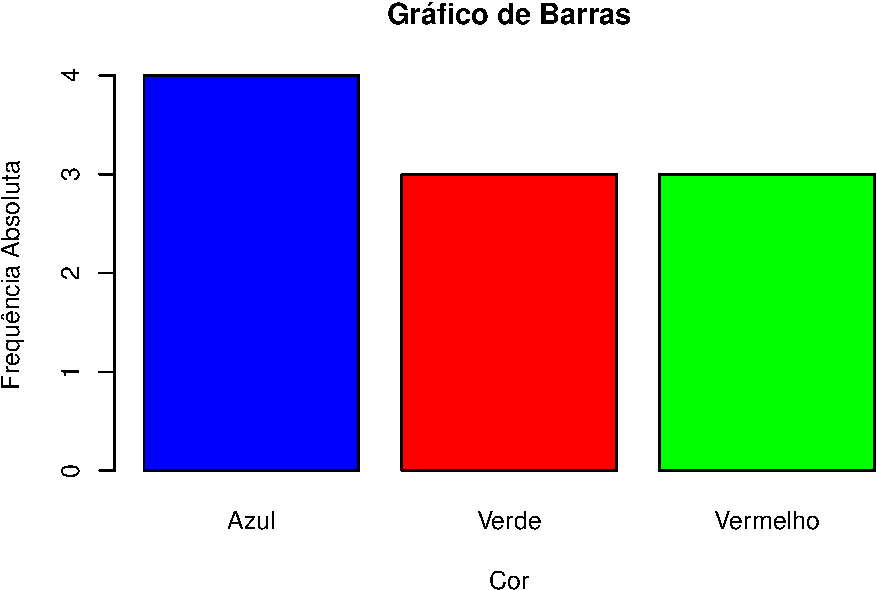
\includegraphics{introR_files/figure-latex/unnamed-chunk-132-1.pdf}

\begin{Shaded}
\begin{Highlighting}[]
\CommentTok{\# Calcular as frequências relativas}
\NormalTok{frequencia\_relativa }\OtherTok{\textless{}{-}}\NormalTok{ frequencia\_absoluta }\SpecialCharTok{/} \FunctionTok{length}\NormalTok{(cores)  }
    
\CommentTok{\# Criar o gráfico de barras com frequências relativas}
\FunctionTok{barplot}\NormalTok{(frequencia\_relativa,         }
  \AttributeTok{main =} \StringTok{"Gráfico de Barras"}\NormalTok{,         }
  \AttributeTok{xlab =} \StringTok{"Cor"}\NormalTok{,         }
  \AttributeTok{ylab =} \StringTok{"Frequência Relativa"}\NormalTok{) }
\end{Highlighting}
\end{Shaded}

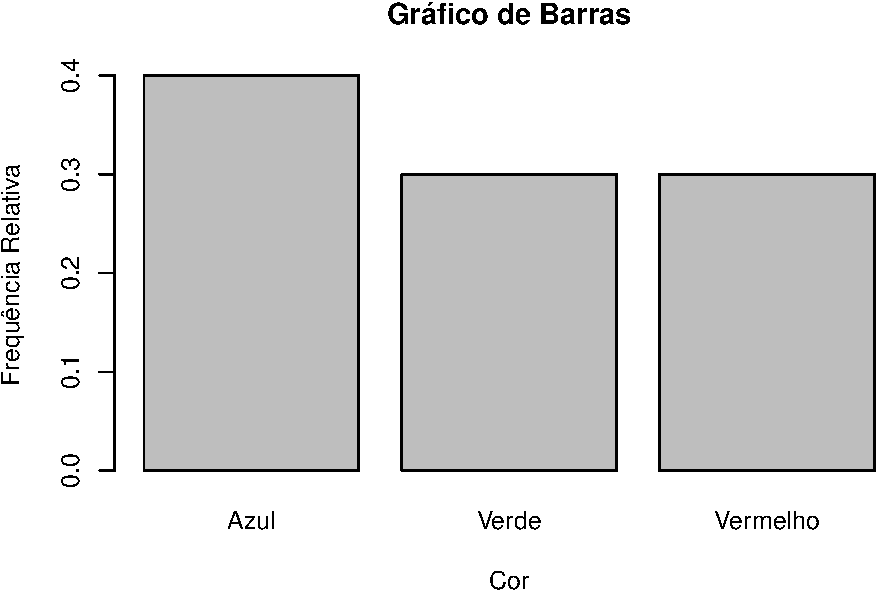
\includegraphics{introR_files/figure-latex/unnamed-chunk-133-1.pdf}

\section{Gráfico circular (pizza)}\label{gruxe1fico-circular-pizza}

\textbf{Gráfico circular}: Exibe as proporções ou percentagens de diferentes
categorias de dados em relação a um todo. Cada categoria é representada
como uma ``fatia'' do círculo, e o tamanho de cada fatia é proporcional à
sua contribuição para o total.

\begin{Shaded}
\begin{Highlighting}[]
\CommentTok{\# Criar gráfico circular}
\FunctionTok{pie}\NormalTok{(frequencia\_relativa, }\AttributeTok{main=}\StringTok{"Gráfico circular"}\NormalTok{,}
  \AttributeTok{col=}\FunctionTok{c}\NormalTok{(}\StringTok{"blue"}\NormalTok{,}\StringTok{"green"}\NormalTok{,}\StringTok{"red"}\NormalTok{))}
\end{Highlighting}
\end{Shaded}

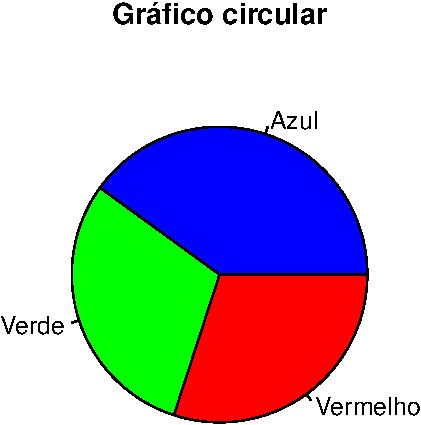
\includegraphics{introR_files/figure-latex/unnamed-chunk-134-1.pdf}

\section{Histograma}\label{histograma}

Histograma é uma representação gráfica dos dados em que se marcam as
classes (intervalos) no eixo horizontal e as frequências (absuluta ou
relativa) no eixo vertical.

\begin{itemize}
\item
  Cada retângulo corresponde a uma classe.
\item
  A largura de cada retângulo é igual à amplitude da classe
\item
  Se as classes tiverem todas a mesma amplitude, a altura do retângulo
  é proporcional à frequência.
\end{itemize}

Por default, o R utiliza a frequência absoluta para construir o
histograma. Se tiver interesse em representar as frequências relativas,
utilize a opção \texttt{freq=FALSE} nos argumentos da função \texttt{hist()}. O padrão
de intervalo de classe no R é \((a, b]\).

\begin{Shaded}
\begin{Highlighting}[]
\CommentTok{\# Considere os dados referentes à massa (em kg) de 40 bicicletas}

\NormalTok{bicicletas }\OtherTok{\textless{}{-}} \FunctionTok{c}\NormalTok{(}\FloatTok{4.3}\NormalTok{,}\FloatTok{6.8}\NormalTok{,}\FloatTok{9.2}\NormalTok{,}\FloatTok{7.2}\NormalTok{,}\FloatTok{8.7}\NormalTok{,}\FloatTok{8.6}\NormalTok{,}\FloatTok{6.6}\NormalTok{,}\FloatTok{5.2}\NormalTok{,}\FloatTok{8.1}\NormalTok{,}\FloatTok{10.9}\NormalTok{,}\FloatTok{7.4}\NormalTok{,}\FloatTok{4.5}\NormalTok{,}\FloatTok{3.8}\NormalTok{,}\FloatTok{7.6}\NormalTok{,}\FloatTok{6.8}\NormalTok{,}\FloatTok{7.8}\NormalTok{,}\FloatTok{8.4}\NormalTok{,}\FloatTok{7.5}\NormalTok{,}\FloatTok{10.5}\NormalTok{,}\FloatTok{6.0}\NormalTok{,}\FloatTok{7.7}\NormalTok{,}\FloatTok{8.1}\NormalTok{,}\FloatTok{7.0}\NormalTok{,}\FloatTok{8.2}\NormalTok{,}\FloatTok{8.4}\NormalTok{,}\FloatTok{8.8}\NormalTok{,}\FloatTok{6.7}\NormalTok{,}\FloatTok{8.2}\NormalTok{,}\FloatTok{9.4}\NormalTok{,}\FloatTok{7.7}\NormalTok{,}\FloatTok{6.3}\NormalTok{,}\FloatTok{7.7}\NormalTok{,}\FloatTok{9.1}\NormalTok{,}\FloatTok{7.9}\NormalTok{,}\FloatTok{7.9}\NormalTok{,}\FloatTok{9.4}\NormalTok{,}\FloatTok{8.2}\NormalTok{,}\FloatTok{6.7}\NormalTok{,}\FloatTok{8.2}\NormalTok{,}\FloatTok{6.5}\NormalTok{)}
  
\NormalTok{h }\OtherTok{\textless{}{-}} \FunctionTok{hist}\NormalTok{(bicicletas,     }
  \AttributeTok{main =} \StringTok{"Histograma"}\NormalTok{,     }
  \AttributeTok{xlab =} \StringTok{"Massa (kg)"}\NormalTok{,     }
  \AttributeTok{ylab =} \StringTok{"Freq. absoluta"}\NormalTok{,     }
  \AttributeTok{ylim =} \FunctionTok{c}\NormalTok{(}\DecValTok{0}\NormalTok{,}\DecValTok{12}\NormalTok{),     }
  \AttributeTok{labels =} \ConstantTok{TRUE}\NormalTok{,     }
  \AttributeTok{col =} \StringTok{"lightblue"}\NormalTok{)}
\end{Highlighting}
\end{Shaded}

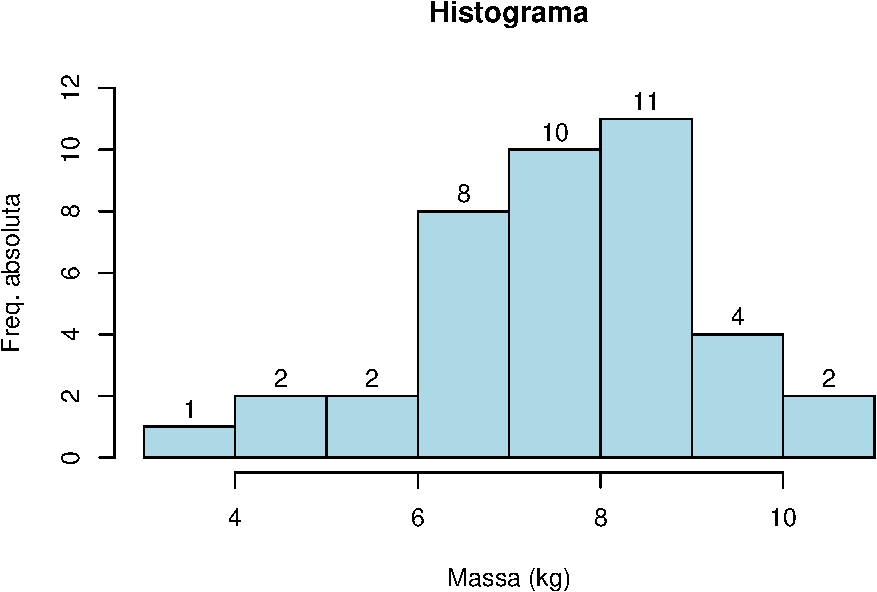
\includegraphics{introR_files/figure-latex/unnamed-chunk-135-1.pdf}

\begin{Shaded}
\begin{Highlighting}[]
\CommentTok{\# Pontos limites das classes}
\NormalTok{h}\SpecialCharTok{$}\NormalTok{breaks}
\DocumentationTok{\#\# [1]  3  4  5  6  7  8  9 10 11}

\CommentTok{\# O comando h$counts retorna um vetor com as frequências absolutas dentro de cada classe}
\NormalTok{h}\SpecialCharTok{$}\NormalTok{counts}
\DocumentationTok{\#\# [1]  1  2  2  8 10 11  4  2}
\end{Highlighting}
\end{Shaded}

\begin{Shaded}
\begin{Highlighting}[]
\CommentTok{\# Histograma com frequência relativa}
\FunctionTok{hist}\NormalTok{(bicicletas,}
  \AttributeTok{main =} \StringTok{"Histograma"}\NormalTok{,          }
  \AttributeTok{xlab =} \StringTok{"Massa (kg)"}\NormalTok{,          }
  \AttributeTok{ylab =} \StringTok{"Freq. relativa"}\NormalTok{,     }
  \AttributeTok{freq =} \ConstantTok{FALSE}\NormalTok{,     }
  \AttributeTok{labels =} \ConstantTok{TRUE}\NormalTok{,          }
  \AttributeTok{col =} \StringTok{"lightblue"}\NormalTok{)}
\end{Highlighting}
\end{Shaded}

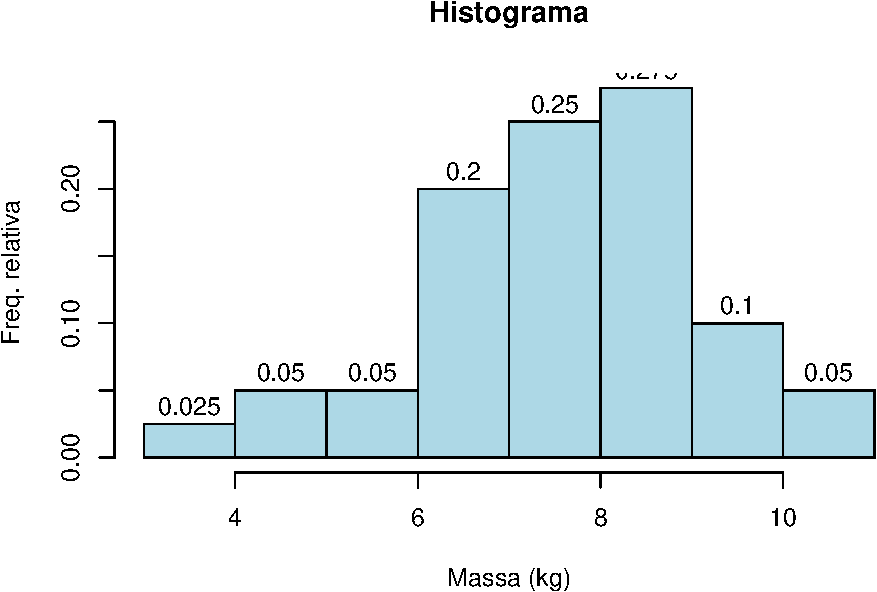
\includegraphics{introR_files/figure-latex/unnamed-chunk-137-1.pdf}

\section{Box-plot}\label{box-plot}

\begin{Shaded}
\begin{Highlighting}[]
\CommentTok{\# Caixa de bigodes vertical}
\FunctionTok{boxplot}\NormalTok{(bicicletas, }\AttributeTok{main =} \StringTok{"Caixa de bigodes"}\NormalTok{, }\AttributeTok{col=}\StringTok{"red"}\NormalTok{)}
\end{Highlighting}
\end{Shaded}

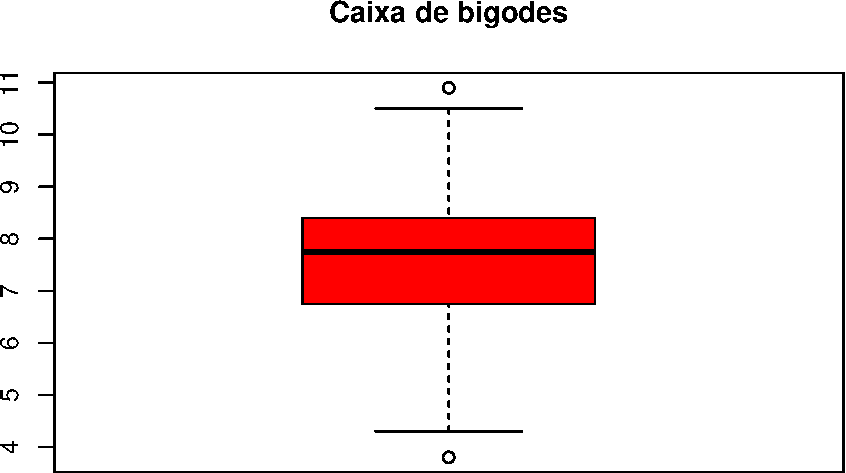
\includegraphics{introR_files/figure-latex/unnamed-chunk-138-1.pdf}

\begin{Shaded}
\begin{Highlighting}[]
\CommentTok{\# Caixa de bigodes horizontal}
\FunctionTok{boxplot}\NormalTok{(bicicletas, }\AttributeTok{main =} \StringTok{"Caixa de bigodes"}\NormalTok{, }\AttributeTok{col=}\StringTok{"green"}\NormalTok{, }\AttributeTok{horizontal =} \ConstantTok{TRUE}\NormalTok{)}
\end{Highlighting}
\end{Shaded}

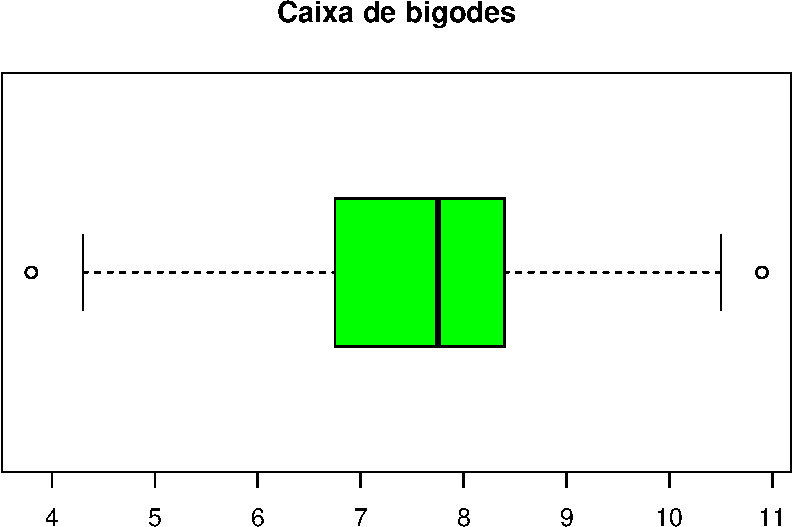
\includegraphics{introR_files/figure-latex/unnamed-chunk-139-1.pdf}

\begin{Shaded}
\begin{Highlighting}[]
\CommentTok{\# Caixa de bigodes lado a lado}
\FunctionTok{par}\NormalTok{(}\AttributeTok{mfrow=}\FunctionTok{c}\NormalTok{(}\DecValTok{1}\NormalTok{,}\DecValTok{2}\NormalTok{))}

\CommentTok{\# Caixa de bigodes vertical}
\FunctionTok{boxplot}\NormalTok{(bicicletas,}\AttributeTok{main =} \StringTok{"Caixa de bigodes"}\NormalTok{,}\AttributeTok{col =} \StringTok{"red"}\NormalTok{)}

\CommentTok{\# Caixa de bigodes horizontal}
\FunctionTok{boxplot}\NormalTok{(bicicletas,}\AttributeTok{main =} \StringTok{"Caixa de bigodes"}\NormalTok{,}\AttributeTok{col =} \StringTok{"green"}\NormalTok{,}\AttributeTok{horizontal =} \ConstantTok{TRUE}\NormalTok{)}
\end{Highlighting}
\end{Shaded}

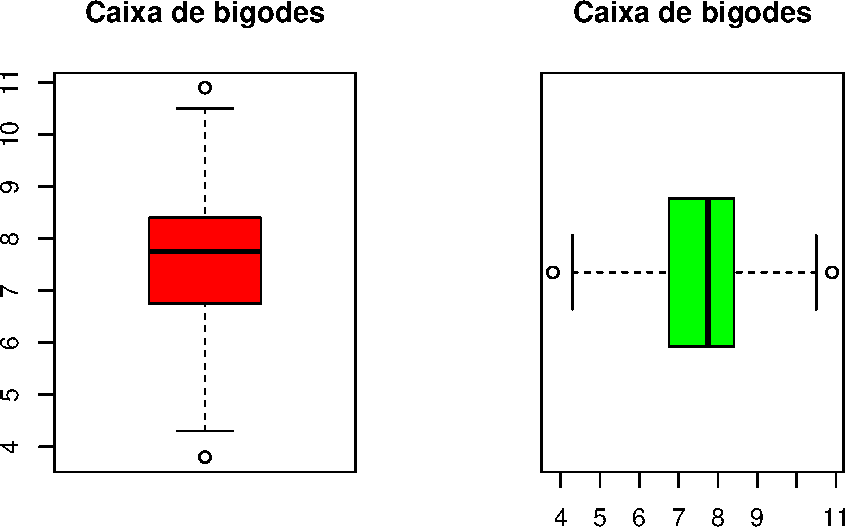
\includegraphics{introR_files/figure-latex/unnamed-chunk-140-1.pdf}

\begin{Shaded}
\begin{Highlighting}[]
\FunctionTok{dev.off}\NormalTok{()}
\end{Highlighting}
\end{Shaded}

\begin{verbatim}
## null device 
##           1
\end{verbatim}

\chapter{Manipulação de dados}\label{manipulauxe7uxe3o-de-dados}

\section{Tibbles}\label{tibbles}

\textbf{Tibbles} são uma versão aprimorada dos data frames no R, introduzida pelo pacote \texttt{tibble}, que faz parte do \texttt{tidyverse}, um conjunto de pacotes projetados para a ciência de dados. Um tibble fornece uma estrutura de dados mais moderna e amigável, melhorando a experiência de manipulação de dados no R.

\textbf{Diferenças Principais entre Tibble e Data Frame}

\begin{longtable}[]{@{}
  >{\raggedright\arraybackslash}p{(\columnwidth - 4\tabcolsep) * \real{0.2847}}
  >{\raggedright\arraybackslash}p{(\columnwidth - 4\tabcolsep) * \real{0.3504}}
  >{\raggedright\arraybackslash}p{(\columnwidth - 4\tabcolsep) * \real{0.3650}}@{}}
\toprule\noalign{}
\begin{minipage}[b]{\linewidth}\raggedright
Característica
\end{minipage} & \begin{minipage}[b]{\linewidth}\raggedright
Data Frame
\end{minipage} & \begin{minipage}[b]{\linewidth}\raggedright
Tibble
\end{minipage} \\
\midrule\noalign{}
\endhead
\bottomrule\noalign{}
\endlastfoot
Impressão no Console & Exibe todos os dados & Exibe um resumo com 10 linhas e colunas visíveis \\
Conversão de Strings & Converte strings para fatores por padrão & Mantém strings como caracteres \\
Manuseio de Colunas & Apenas vetores, listas podem ser problemáticas & Permite listas, funções, outros tibbles \\
Nomes de Colunas & Nomes devem ser únicos e sem espaços & Nomes podem ter espaços, ser duplicados, etc. \\
Retorno de Subsetting (\texttt{{[}}) & Pode retornar um vetor ou data frame & Sempre retorna um tibble \\
Compatibilidade e Integração & Totalmente compatível com base R & Compatível, mas otimizado para uso com tidyverse \\
Manipulação de Dados & Pode ser menos intuitivo para algumas operações & Mais amigável e intuitivo, especialmente com pipes \\
\end{longtable}

\begin{Shaded}
\begin{Highlighting}[]
\FunctionTok{library}\NormalTok{(tibble)}

\CommentTok{\# Criando um tibble}
\NormalTok{tb }\OtherTok{\textless{}{-}} \FunctionTok{tibble}\NormalTok{(}
  \AttributeTok{x =} \DecValTok{1}\SpecialCharTok{:}\DecValTok{5}\NormalTok{,}
  \AttributeTok{y =} \FunctionTok{c}\NormalTok{(}\StringTok{"A"}\NormalTok{, }\StringTok{"B"}\NormalTok{, }\StringTok{"C"}\NormalTok{, }\StringTok{"D"}\NormalTok{, }\StringTok{"E"}\NormalTok{),}
  \AttributeTok{z =}\NormalTok{ x }\SpecialCharTok{*} \DecValTok{2}
\NormalTok{)}

\FunctionTok{print}\NormalTok{(tb)}
\DocumentationTok{\#\# \# A tibble: 5 × 3}
\DocumentationTok{\#\#       x y         z}
\DocumentationTok{\#\#   \textless{}int\textgreater{} \textless{}chr\textgreater{} \textless{}dbl\textgreater{}}
\DocumentationTok{\#\# 1     1 A         2}
\DocumentationTok{\#\# 2     2 B         4}
\DocumentationTok{\#\# 3     3 C         6}
\DocumentationTok{\#\# 4     4 D         8}
\DocumentationTok{\#\# 5     5 E        10}
\end{Highlighting}
\end{Shaded}

Conversão de data frame pra tibble:

\begin{Shaded}
\begin{Highlighting}[]
\CommentTok{\# Criando um data frame}
\NormalTok{df }\OtherTok{\textless{}{-}} \FunctionTok{data.frame}\NormalTok{(}
  \AttributeTok{x =} \DecValTok{1}\SpecialCharTok{:}\DecValTok{5}\NormalTok{,}
  \AttributeTok{y =} \FunctionTok{c}\NormalTok{(}\StringTok{"A"}\NormalTok{, }\StringTok{"B"}\NormalTok{, }\StringTok{"C"}\NormalTok{, }\StringTok{"D"}\NormalTok{, }\StringTok{"E"}\NormalTok{)}
\NormalTok{)}

\CommentTok{\# Convertendo para tibble}
\NormalTok{tb }\OtherTok{\textless{}{-}} \FunctionTok{as\_tibble}\NormalTok{(df)}

\FunctionTok{print}\NormalTok{(tb)}
\DocumentationTok{\#\# \# A tibble: 5 × 2}
\DocumentationTok{\#\#       x y    }
\DocumentationTok{\#\#   \textless{}int\textgreater{} \textless{}chr\textgreater{}}
\DocumentationTok{\#\# 1     1 A    }
\DocumentationTok{\#\# 2     2 B    }
\DocumentationTok{\#\# 3     3 C    }
\DocumentationTok{\#\# 4     4 D    }
\DocumentationTok{\#\# 5     5 E}
\end{Highlighting}
\end{Shaded}

\section{\texorpdfstring{O pacote \texttt{dplyr}}{O pacote dplyr}}\label{o-pacote-dplyr}

O \texttt{dplyr} é um dos pacotes mais populares e amplamente utilizados no R
para manipulação e transformação de dados. Ele faz parte do conjunto de
pacotes ``tidyverse,'' que são projetados para simplificar o trabalho com
dados no R. O \texttt{dplyr} oferece uma interface intuitiva e de fácil uso
para realizar operações comuns em data frames, como seleção de colunas,
filtragem de linhas, ordenação, resumo de dados e junção de data frames.

As principais funções do \texttt{dplyr} são:

\begin{itemize}
\tightlist
\item
  \texttt{select()} - seleciona colunas
\item
  \texttt{arrange()} - ordena a base
\item
  \texttt{filter()} - filtra linhas
\item
  \texttt{mutate()} - cria/modifica colunas
\item
  \texttt{group\_by()} - agrupa a base
\item
  \texttt{summarise()} - sumariza a base
\end{itemize}

Neste capítulo, vamos trabalhar com uma base de dados do Star Wars. Essa
base está disponível dentro do pacote \texttt{dplyr} no R e pode ser acessada
através do comando \texttt{starwars}.

Assim, utilizaremos o objeto \texttt{sw} para acessar os dados.

\begin{Shaded}
\begin{Highlighting}[]
\FunctionTok{library}\NormalTok{(dplyr)}
\end{Highlighting}
\end{Shaded}

\begin{verbatim}
## 
## Attaching package: 'dplyr'
\end{verbatim}

\begin{verbatim}
## The following objects are masked from 'package:stats':
## 
##     filter, lag
\end{verbatim}

\begin{verbatim}
## The following objects are masked from 'package:base':
## 
##     intersect, setdiff, setequal, union
\end{verbatim}

\begin{Shaded}
\begin{Highlighting}[]
\NormalTok{sw }\OtherTok{\textless{}{-}}\NormalTok{ starwars}
\NormalTok{sw}
\end{Highlighting}
\end{Shaded}

\begin{verbatim}
## # A tibble: 87 x 14
##    name     height  mass hair_color skin_color eye_color birth_year sex   gender
##    <chr>     <int> <dbl> <chr>      <chr>      <chr>          <dbl> <chr> <chr> 
##  1 Luke Sk~    172    77 blond      fair       blue            19   male  mascu~
##  2 C-3PO       167    75 <NA>       gold       yellow         112   none  mascu~
##  3 R2-D2        96    32 <NA>       white, bl~ red             33   none  mascu~
##  4 Darth V~    202   136 none       white      yellow          41.9 male  mascu~
##  5 Leia Or~    150    49 brown      light      brown           19   fema~ femin~
##  6 Owen La~    178   120 brown, gr~ light      blue            52   male  mascu~
##  7 Beru Wh~    165    75 brown      light      blue            47   fema~ femin~
##  8 R5-D4        97    32 <NA>       white, red red             NA   none  mascu~
##  9 Biggs D~    183    84 black      light      brown           24   male  mascu~
## 10 Obi-Wan~    182    77 auburn, w~ fair       blue-gray       57   male  mascu~
## # i 77 more rows
## # i 5 more variables: homeworld <chr>, species <chr>, films <list>,
## #   vehicles <list>, starships <list>
\end{verbatim}

\subsection{Selecionando colunas}\label{selecionando-colunas}

Para selecionar colunas, utilizamos a função \texttt{select()}. Repare que não
precisamos colocar o nome da coluna entre aspas.

\begin{Shaded}
\begin{Highlighting}[]
\FunctionTok{select}\NormalTok{(sw, name)}
\end{Highlighting}
\end{Shaded}

\begin{verbatim}
## # A tibble: 87 x 1
##    name              
##    <chr>             
##  1 Luke Skywalker    
##  2 C-3PO             
##  3 R2-D2             
##  4 Darth Vader       
##  5 Leia Organa       
##  6 Owen Lars         
##  7 Beru Whitesun Lars
##  8 R5-D4             
##  9 Biggs Darklighter 
## 10 Obi-Wan Kenobi    
## # i 77 more rows
\end{verbatim}

Também podemos selecionar várias colunas

\begin{Shaded}
\begin{Highlighting}[]
\FunctionTok{select}\NormalTok{(sw, name, mass, hair\_color)}
\end{Highlighting}
\end{Shaded}

\begin{verbatim}
## # A tibble: 87 x 3
##    name                mass hair_color   
##    <chr>              <dbl> <chr>        
##  1 Luke Skywalker        77 blond        
##  2 C-3PO                 75 <NA>         
##  3 R2-D2                 32 <NA>         
##  4 Darth Vader          136 none         
##  5 Leia Organa           49 brown        
##  6 Owen Lars            120 brown, grey  
##  7 Beru Whitesun Lars    75 brown        
##  8 R5-D4                 32 <NA>         
##  9 Biggs Darklighter     84 black        
## 10 Obi-Wan Kenobi        77 auburn, white
## # i 77 more rows
\end{verbatim}

Podemos usar o operador \texttt{:} para selecionar colunas consecutivas.

\begin{Shaded}
\begin{Highlighting}[]
\FunctionTok{select}\NormalTok{(sw, name}\SpecialCharTok{:}\NormalTok{hair\_color)}
\end{Highlighting}
\end{Shaded}

\begin{verbatim}
## # A tibble: 87 x 4
##    name               height  mass hair_color   
##    <chr>               <int> <dbl> <chr>        
##  1 Luke Skywalker        172    77 blond        
##  2 C-3PO                 167    75 <NA>         
##  3 R2-D2                  96    32 <NA>         
##  4 Darth Vader           202   136 none         
##  5 Leia Organa           150    49 brown        
##  6 Owen Lars             178   120 brown, grey  
##  7 Beru Whitesun Lars    165    75 brown        
##  8 R5-D4                  97    32 <NA>         
##  9 Biggs Darklighter     183    84 black        
## 10 Obi-Wan Kenobi        182    77 auburn, white
## # i 77 more rows
\end{verbatim}

O \texttt{dplyr} possui um conjunto de funções auxiliares muito úteis para
seleção de colunas. As principais são:

\begin{itemize}
\tightlist
\item
  \texttt{starts\_with()}: para colunas que começam com um texto padrão
\item
  \texttt{ends\_with()}: para colunas que terminam com um texto padrão
\item
  \texttt{contains()}: para colunas que contêm um texto padrão
\end{itemize}

\begin{Shaded}
\begin{Highlighting}[]
\FunctionTok{select}\NormalTok{(sw, }\FunctionTok{ends\_with}\NormalTok{(}\StringTok{"color"}\NormalTok{))}
\end{Highlighting}
\end{Shaded}

\begin{verbatim}
## # A tibble: 87 x 3
##    hair_color    skin_color  eye_color
##    <chr>         <chr>       <chr>    
##  1 blond         fair        blue     
##  2 <NA>          gold        yellow   
##  3 <NA>          white, blue red      
##  4 none          white       yellow   
##  5 brown         light       brown    
##  6 brown, grey   light       blue     
##  7 brown         light       blue     
##  8 <NA>          white, red  red      
##  9 black         light       brown    
## 10 auburn, white fair        blue-gray
## # i 77 more rows
\end{verbatim}

Para remover colunas basta acrescentar um \texttt{-} antes da seleção.

\begin{Shaded}
\begin{Highlighting}[]
\FunctionTok{select}\NormalTok{(sw, }\SpecialCharTok{{-}}\NormalTok{name, }\SpecialCharTok{{-}}\NormalTok{hair\_color)}
\end{Highlighting}
\end{Shaded}

\begin{verbatim}
## # A tibble: 87 x 12
##    height  mass skin_color  eye_color birth_year sex    gender homeworld species
##     <int> <dbl> <chr>       <chr>          <dbl> <chr>  <chr>  <chr>     <chr>  
##  1    172    77 fair        blue            19   male   mascu~ Tatooine  Human  
##  2    167    75 gold        yellow         112   none   mascu~ Tatooine  Droid  
##  3     96    32 white, blue red             33   none   mascu~ Naboo     Droid  
##  4    202   136 white       yellow          41.9 male   mascu~ Tatooine  Human  
##  5    150    49 light       brown           19   female femin~ Alderaan  Human  
##  6    178   120 light       blue            52   male   mascu~ Tatooine  Human  
##  7    165    75 light       blue            47   female femin~ Tatooine  Human  
##  8     97    32 white, red  red             NA   none   mascu~ Tatooine  Droid  
##  9    183    84 light       brown           24   male   mascu~ Tatooine  Human  
## 10    182    77 fair        blue-gray       57   male   mascu~ Stewjon   Human  
## # i 77 more rows
## # i 3 more variables: films <list>, vehicles <list>, starships <list>
\end{verbatim}

\begin{Shaded}
\begin{Highlighting}[]
\FunctionTok{select}\NormalTok{(sw, }\SpecialCharTok{{-}}\FunctionTok{ends\_with}\NormalTok{(}\StringTok{"color"}\NormalTok{))}
\end{Highlighting}
\end{Shaded}

\begin{verbatim}
## # A tibble: 87 x 11
##    name    height  mass birth_year sex   gender homeworld species films vehicles
##    <chr>    <int> <dbl>      <dbl> <chr> <chr>  <chr>     <chr>   <lis> <list>  
##  1 Luke S~    172    77       19   male  mascu~ Tatooine  Human   <chr> <chr>   
##  2 C-3PO      167    75      112   none  mascu~ Tatooine  Droid   <chr> <chr>   
##  3 R2-D2       96    32       33   none  mascu~ Naboo     Droid   <chr> <chr>   
##  4 Darth ~    202   136       41.9 male  mascu~ Tatooine  Human   <chr> <chr>   
##  5 Leia O~    150    49       19   fema~ femin~ Alderaan  Human   <chr> <chr>   
##  6 Owen L~    178   120       52   male  mascu~ Tatooine  Human   <chr> <chr>   
##  7 Beru W~    165    75       47   fema~ femin~ Tatooine  Human   <chr> <chr>   
##  8 R5-D4       97    32       NA   none  mascu~ Tatooine  Droid   <chr> <chr>   
##  9 Biggs ~    183    84       24   male  mascu~ Tatooine  Human   <chr> <chr>   
## 10 Obi-Wa~    182    77       57   male  mascu~ Stewjon   Human   <chr> <chr>   
## # i 77 more rows
## # i 1 more variable: starships <list>
\end{verbatim}

\subsection{Exercícios}\label{exercuxedcios-12}

Utilize a base \texttt{sw} nos exercícios a seguir.

\textbf{1.} Teste aplicar a função \texttt{glimpse()} do pacote `\texttt{dplyr} à base
\texttt{sw}. O que ela faz?

\textbf{2.} Crie uma tabela com apenas as colunas \texttt{name}, \texttt{gender}, e
\texttt{films}. Salve em um objeto chamado \texttt{sw\_simples}.

\textbf{3.} Selecione apenas as colunas \texttt{hair\_color}, \texttt{skin\_color} e
\texttt{eye\_color} usando a função auxiliar \texttt{contains()}.

\textbf{4.} Usando a função \texttt{select()} (e suas funções auxiliares), escreva
códigos que retornem a base \texttt{sw} sem as colunas \texttt{hair\_color},
\texttt{skin\_color} e \texttt{eye\_color}. Escreva todas as soluções diferentes que
você conseguir pensar.

\subsection{Ordenando a base}\label{ordenando-a-base}

Para ordenar linhas, utilizamos a função \texttt{arrange()}. O primeiro
argumento é a base de dados. Os demais argumentos são as colunas pelas
quais queremos ordenar as linhas.

\begin{Shaded}
\begin{Highlighting}[]
\FunctionTok{arrange}\NormalTok{(sw, mass)}
\end{Highlighting}
\end{Shaded}

\begin{verbatim}
## # A tibble: 87 x 14
##    name     height  mass hair_color skin_color eye_color birth_year sex   gender
##    <chr>     <int> <dbl> <chr>      <chr>      <chr>          <dbl> <chr> <chr> 
##  1 Ratts T~     79    15 none       grey, blue unknown           NA male  mascu~
##  2 Yoda         66    17 white      green      brown            896 male  mascu~
##  3 Wicket ~     88    20 brown      brown      brown              8 male  mascu~
##  4 R2-D2        96    32 <NA>       white, bl~ red               33 none  mascu~
##  5 R5-D4        97    32 <NA>       white, red red               NA none  mascu~
##  6 Sebulba     112    40 none       grey, red  orange            NA male  mascu~
##  7 Padmé A~    185    45 brown      light      brown             46 fema~ femin~
##  8 Dud Bolt     94    45 none       blue, grey yellow            NA male  mascu~
##  9 Wat Tam~    193    48 none       green, gr~ unknown           NA male  mascu~
## 10 Sly Moo~    178    48 none       pale       white             NA <NA>  <NA>  
## # i 77 more rows
## # i 5 more variables: homeworld <chr>, species <chr>, films <list>,
## #   vehicles <list>, starships <list>
\end{verbatim}

Também podemos ordenar de forma decrescente usando a função \texttt{desc()}.

\begin{Shaded}
\begin{Highlighting}[]
\FunctionTok{arrange}\NormalTok{(sw, }\FunctionTok{desc}\NormalTok{(mass))}
\end{Highlighting}
\end{Shaded}

\begin{verbatim}
## # A tibble: 87 x 14
##    name     height  mass hair_color skin_color eye_color birth_year sex   gender
##    <chr>     <int> <dbl> <chr>      <chr>      <chr>          <dbl> <chr> <chr> 
##  1 Jabba D~    175  1358 <NA>       green-tan~ orange         600   herm~ mascu~
##  2 Grievous    216   159 none       brown, wh~ green, y~       NA   male  mascu~
##  3 IG-88       200   140 none       metal      red             15   none  mascu~
##  4 Darth V~    202   136 none       white      yellow          41.9 male  mascu~
##  5 Tarfful     234   136 brown      brown      blue            NA   male  mascu~
##  6 Owen La~    178   120 brown, gr~ light      blue            52   male  mascu~
##  7 Bossk       190   113 none       green      red             53   male  mascu~
##  8 Chewbac~    228   112 brown      unknown    blue           200   male  mascu~
##  9 Jek Ton~    180   110 brown      fair       blue            NA   <NA>  <NA>  
## 10 Dexter ~    198   102 none       brown      yellow          NA   male  mascu~
## # i 77 more rows
## # i 5 more variables: homeworld <chr>, species <chr>, films <list>,
## #   vehicles <list>, starships <list>
\end{verbatim}

Ordenar segundo duas ou mais colunas.

\begin{Shaded}
\begin{Highlighting}[]
\FunctionTok{arrange}\NormalTok{(sw, }\FunctionTok{desc}\NormalTok{(height), }\FunctionTok{desc}\NormalTok{(mass))}
\end{Highlighting}
\end{Shaded}

\begin{verbatim}
## # A tibble: 87 x 14
##    name     height  mass hair_color skin_color eye_color birth_year sex   gender
##    <chr>     <int> <dbl> <chr>      <chr>      <chr>          <dbl> <chr> <chr> 
##  1 Yarael ~    264    NA none       white      yellow          NA   male  mascu~
##  2 Tarfful     234   136 brown      brown      blue            NA   male  mascu~
##  3 Lama Su     229    88 none       grey       black           NA   male  mascu~
##  4 Chewbac~    228   112 brown      unknown    blue           200   male  mascu~
##  5 Roos Ta~    224    82 none       grey       orange          NA   male  mascu~
##  6 Grievous    216   159 none       brown, wh~ green, y~       NA   male  mascu~
##  7 Taun We     213    NA none       grey       black           NA   fema~ femin~
##  8 Tion Me~    206    80 none       grey       black           NA   male  mascu~
##  9 Rugor N~    206    NA none       green      orange          NA   male  mascu~
## 10 Darth V~    202   136 none       white      yellow          41.9 male  mascu~
## # i 77 more rows
## # i 5 more variables: homeworld <chr>, species <chr>, films <list>,
## #   vehicles <list>, starships <list>
\end{verbatim}

\subsection{Exercícios}\label{exercuxedcios-13}

\textbf{1.} Ordene \texttt{mass} em ordem crescente e \texttt{birth\_year} em ordem
decrescente e salve em um objeto chamado \texttt{sw\_ordenados}.

\begin{Shaded}
\begin{Highlighting}[]
\NormalTok{sw\_ordenados }\OtherTok{\textless{}{-}} \FunctionTok{arrange}\NormalTok{(sw, mass, }\FunctionTok{desc}\NormalTok{(birth\_year))}
\NormalTok{sw\_ordenados}
\end{Highlighting}
\end{Shaded}

\textbf{2.} Selecione apenas as colunas \texttt{name} e \texttt{birth\_year} e então ordene
de forma decrescente pelo \texttt{birth\_year}.

\begin{Shaded}
\begin{Highlighting}[]
\CommentTok{\# Aninhando funções}
\FunctionTok{arrange}\NormalTok{(}\FunctionTok{select}\NormalTok{(sw, name, birth\_year), }\FunctionTok{desc}\NormalTok{(birth\_year))}

\CommentTok{\# Criando um objeto intermediário}
\NormalTok{sw\_aux }\OtherTok{\textless{}{-}} \FunctionTok{select}\NormalTok{(sw, name, birth\_year)}
\FunctionTok{arrange}\NormalTok{(sw\_aux, }\FunctionTok{desc}\NormalTok{(birth\_year))}

\CommentTok{\# Pipe}
\NormalTok{sw }\SpecialCharTok{\%\textgreater{}\%} 
  \FunctionTok{select}\NormalTok{(name, birth\_year) }\SpecialCharTok{\%\textgreater{}\%} 
  \FunctionTok{arrange}\NormalTok{(}\FunctionTok{desc}\NormalTok{(birth\_year))}
\end{Highlighting}
\end{Shaded}

\subsection{Filtrando linhas}\label{filtrando-linhas}

Para filtrar valores de uma coluna da base, utilizamos a função
\texttt{filter()}.

\begin{Shaded}
\begin{Highlighting}[]
\CommentTok{\# filter(sw, height \textgreater{} 170)}
\CommentTok{\# Ou}
\NormalTok{sw }\SpecialCharTok{\%\textgreater{}\%} \FunctionTok{filter}\NormalTok{(height }\SpecialCharTok{\textgreater{}} \DecValTok{170}\NormalTok{)}
\end{Highlighting}
\end{Shaded}

\begin{verbatim}
## # A tibble: 55 x 14
##    name     height  mass hair_color skin_color eye_color birth_year sex   gender
##    <chr>     <int> <dbl> <chr>      <chr>      <chr>          <dbl> <chr> <chr> 
##  1 Luke Sk~    172    77 blond      fair       blue            19   male  mascu~
##  2 Darth V~    202   136 none       white      yellow          41.9 male  mascu~
##  3 Owen La~    178   120 brown, gr~ light      blue            52   male  mascu~
##  4 Biggs D~    183    84 black      light      brown           24   male  mascu~
##  5 Obi-Wan~    182    77 auburn, w~ fair       blue-gray       57   male  mascu~
##  6 Anakin ~    188    84 blond      fair       blue            41.9 male  mascu~
##  7 Wilhuff~    180    NA auburn, g~ fair       blue            64   male  mascu~
##  8 Chewbac~    228   112 brown      unknown    blue           200   male  mascu~
##  9 Han Solo    180    80 brown      fair       brown           29   male  mascu~
## 10 Greedo      173    74 <NA>       green      black           44   male  mascu~
## # i 45 more rows
## # i 5 more variables: homeworld <chr>, species <chr>, films <list>,
## #   vehicles <list>, starships <list>
\end{verbatim}

Podemos selecionar apenas as colunas \texttt{name} e \texttt{height} para
visualizarmos as alturas:

\begin{Shaded}
\begin{Highlighting}[]
\NormalTok{sw }\SpecialCharTok{\%\textgreater{}\%} 
  \FunctionTok{filter}\NormalTok{(height }\SpecialCharTok{\textgreater{}} \DecValTok{170}\NormalTok{) }\SpecialCharTok{\%\textgreater{}\%} 
  \FunctionTok{select}\NormalTok{(name, height)}
\end{Highlighting}
\end{Shaded}

\begin{verbatim}
## # A tibble: 55 x 2
##    name              height
##    <chr>              <int>
##  1 Luke Skywalker       172
##  2 Darth Vader          202
##  3 Owen Lars            178
##  4 Biggs Darklighter    183
##  5 Obi-Wan Kenobi       182
##  6 Anakin Skywalker     188
##  7 Wilhuff Tarkin       180
##  8 Chewbacca            228
##  9 Han Solo             180
## 10 Greedo               173
## # i 45 more rows
\end{verbatim}

Podemos estender o filtro para duas ou mais colunas.

\begin{Shaded}
\begin{Highlighting}[]
\FunctionTok{filter}\NormalTok{(sw, height}\SpecialCharTok{\textgreater{}}\DecValTok{170}\NormalTok{, mass}\SpecialCharTok{\textgreater{}}\DecValTok{80}\NormalTok{)}
\end{Highlighting}
\end{Shaded}

\begin{verbatim}
## # A tibble: 21 x 14
##    name     height  mass hair_color skin_color eye_color birth_year sex   gender
##    <chr>     <int> <dbl> <chr>      <chr>      <chr>          <dbl> <chr> <chr> 
##  1 Darth V~    202   136 none       white      yellow          41.9 male  mascu~
##  2 Owen La~    178   120 brown, gr~ light      blue            52   male  mascu~
##  3 Biggs D~    183    84 black      light      brown           24   male  mascu~
##  4 Anakin ~    188    84 blond      fair       blue            41.9 male  mascu~
##  5 Chewbac~    228   112 brown      unknown    blue           200   male  mascu~
##  6 Jabba D~    175  1358 <NA>       green-tan~ orange         600   herm~ mascu~
##  7 Jek Ton~    180   110 brown      fair       blue            NA   <NA>  <NA>  
##  8 IG-88       200   140 none       metal      red             15   none  mascu~
##  9 Bossk       190   113 none       green      red             53   male  mascu~
## 10 Ackbar      180    83 none       brown mot~ orange          41   male  mascu~
## # i 11 more rows
## # i 5 more variables: homeworld <chr>, species <chr>, films <list>,
## #   vehicles <list>, starships <list>
\end{verbatim}

\begin{Shaded}
\begin{Highlighting}[]
\NormalTok{sw }\SpecialCharTok{\%\textgreater{}\%} \FunctionTok{filter}\NormalTok{(height }\SpecialCharTok{\textgreater{}} \DecValTok{170}\NormalTok{, mass }\SpecialCharTok{\textgreater{}} \DecValTok{80}\NormalTok{)}
\end{Highlighting}
\end{Shaded}

\begin{verbatim}
## # A tibble: 21 x 14
##    name     height  mass hair_color skin_color eye_color birth_year sex   gender
##    <chr>     <int> <dbl> <chr>      <chr>      <chr>          <dbl> <chr> <chr> 
##  1 Darth V~    202   136 none       white      yellow          41.9 male  mascu~
##  2 Owen La~    178   120 brown, gr~ light      blue            52   male  mascu~
##  3 Biggs D~    183    84 black      light      brown           24   male  mascu~
##  4 Anakin ~    188    84 blond      fair       blue            41.9 male  mascu~
##  5 Chewbac~    228   112 brown      unknown    blue           200   male  mascu~
##  6 Jabba D~    175  1358 <NA>       green-tan~ orange         600   herm~ mascu~
##  7 Jek Ton~    180   110 brown      fair       blue            NA   <NA>  <NA>  
##  8 IG-88       200   140 none       metal      red             15   none  mascu~
##  9 Bossk       190   113 none       green      red             53   male  mascu~
## 10 Ackbar      180    83 none       brown mot~ orange          41   male  mascu~
## # i 11 more rows
## # i 5 more variables: homeworld <chr>, species <chr>, films <list>,
## #   vehicles <list>, starships <list>
\end{verbatim}

Podemos filtrar colunas categóricas. O exemplo abaixo retorna uma tabela
apenas com os personagens com cabelo preto ou castanho.

\begin{Shaded}
\begin{Highlighting}[]
\FunctionTok{filter}\NormalTok{(sw, hair\_color }\SpecialCharTok{==} \StringTok{"black"} \SpecialCharTok{|}\NormalTok{ hair\_color }\SpecialCharTok{==} \StringTok{"brown"}\NormalTok{)}
\end{Highlighting}
\end{Shaded}

\begin{verbatim}
## # A tibble: 31 x 14
##    name     height  mass hair_color skin_color eye_color birth_year sex   gender
##    <chr>     <int> <dbl> <chr>      <chr>      <chr>          <dbl> <chr> <chr> 
##  1 Leia Or~    150  49   brown      light      brown           19   fema~ femin~
##  2 Beru Wh~    165  75   brown      light      blue            47   fema~ femin~
##  3 Biggs D~    183  84   black      light      brown           24   male  mascu~
##  4 Chewbac~    228 112   brown      unknown    blue           200   male  mascu~
##  5 Han Solo    180  80   brown      fair       brown           29   male  mascu~
##  6 Wedge A~    170  77   brown      fair       hazel           21   male  mascu~
##  7 Jek Ton~    180 110   brown      fair       blue            NA   <NA>  <NA>  
##  8 Boba Fe~    183  78.2 black      fair       brown           31.5 male  mascu~
##  9 Lando C~    177  79   black      dark       brown           31   male  mascu~
## 10 Arvel C~     NA  NA   brown      fair       brown           NA   male  mascu~
## # i 21 more rows
## # i 5 more variables: homeworld <chr>, species <chr>, films <list>,
## #   vehicles <list>, starships <list>
\end{verbatim}

\begin{Shaded}
\begin{Highlighting}[]
\NormalTok{sw }\SpecialCharTok{\%\textgreater{}\%} \FunctionTok{filter}\NormalTok{(hair\_color }\SpecialCharTok{\%in\%} \FunctionTok{c}\NormalTok{(}\StringTok{"black"}\NormalTok{,}\StringTok{"brown"}\NormalTok{))}
\end{Highlighting}
\end{Shaded}

\begin{verbatim}
## # A tibble: 31 x 14
##    name     height  mass hair_color skin_color eye_color birth_year sex   gender
##    <chr>     <int> <dbl> <chr>      <chr>      <chr>          <dbl> <chr> <chr> 
##  1 Leia Or~    150  49   brown      light      brown           19   fema~ femin~
##  2 Beru Wh~    165  75   brown      light      blue            47   fema~ femin~
##  3 Biggs D~    183  84   black      light      brown           24   male  mascu~
##  4 Chewbac~    228 112   brown      unknown    blue           200   male  mascu~
##  5 Han Solo    180  80   brown      fair       brown           29   male  mascu~
##  6 Wedge A~    170  77   brown      fair       hazel           21   male  mascu~
##  7 Jek Ton~    180 110   brown      fair       blue            NA   <NA>  <NA>  
##  8 Boba Fe~    183  78.2 black      fair       brown           31.5 male  mascu~
##  9 Lando C~    177  79   black      dark       brown           31   male  mascu~
## 10 Arvel C~     NA  NA   brown      fair       brown           NA   male  mascu~
## # i 21 more rows
## # i 5 more variables: homeworld <chr>, species <chr>, films <list>,
## #   vehicles <list>, starships <list>
\end{verbatim}

Para filtrar textos sem correspondência exata, podemos utilizar a função
auxiliar \texttt{str\_detect()} do pacote \texttt{\{stringr\}}. Ela serve para verificar
se cada string de um vetor contém um determinado padrão de texto.

\begin{Shaded}
\begin{Highlighting}[]
\FunctionTok{library}\NormalTok{(stringr)}

\FunctionTok{str\_detect}\NormalTok{(}
  \AttributeTok{string =} \FunctionTok{c}\NormalTok{(}\StringTok{"a"}\NormalTok{, }\StringTok{"aa"}\NormalTok{,}\StringTok{"abc"}\NormalTok{, }\StringTok{"bc"}\NormalTok{, }\StringTok{"A"}\NormalTok{, }\ConstantTok{NA}\NormalTok{), }
  \AttributeTok{pattern =} \StringTok{"a"}
\NormalTok{)}
\end{Highlighting}
\end{Shaded}

\begin{verbatim}
## [1]  TRUE  TRUE  TRUE FALSE FALSE    NA
\end{verbatim}

Podemos utilizá-la para filtrar apenas os personagens com cabelo \texttt{grey}.

\begin{Shaded}
\begin{Highlighting}[]
\CommentTok{\# Podemos detectar se o cabelo grey aparece na string}
\FunctionTok{str\_detect}\NormalTok{(}
  \AttributeTok{string =}\NormalTok{ sw}\SpecialCharTok{$}\NormalTok{hair\_color,}
  \AttributeTok{pattern =} \StringTok{"grey"}
\NormalTok{)}
\end{Highlighting}
\end{Shaded}

\begin{verbatim}
##  [1] FALSE    NA    NA FALSE FALSE  TRUE FALSE    NA FALSE FALSE FALSE  TRUE
## [13] FALSE FALSE    NA    NA FALSE FALSE FALSE  TRUE FALSE FALSE FALSE FALSE
## [25] FALSE FALSE FALSE FALSE FALSE FALSE FALSE FALSE FALSE FALSE FALSE FALSE
## [37] FALSE FALSE FALSE FALSE FALSE FALSE FALSE FALSE FALSE FALSE FALSE FALSE
## [49] FALSE FALSE FALSE FALSE FALSE FALSE FALSE FALSE FALSE FALSE FALSE FALSE
## [61] FALSE FALSE FALSE FALSE FALSE FALSE FALSE FALSE FALSE FALSE FALSE FALSE
## [73] FALSE FALSE FALSE FALSE FALSE FALSE FALSE FALSE FALSE FALSE FALSE FALSE
## [85] FALSE FALSE FALSE
\end{verbatim}

\begin{Shaded}
\begin{Highlighting}[]
\FunctionTok{library}\NormalTok{(stringr)}
\NormalTok{sw }\SpecialCharTok{\%\textgreater{}\%} \FunctionTok{filter}\NormalTok{(}\FunctionTok{str\_detect}\NormalTok{(hair\_color,}\StringTok{"grey"}\NormalTok{))}
\end{Highlighting}
\end{Shaded}

\begin{verbatim}
## # A tibble: 3 x 14
##   name      height  mass hair_color skin_color eye_color birth_year sex   gender
##   <chr>      <int> <dbl> <chr>      <chr>      <chr>          <dbl> <chr> <chr> 
## 1 Owen Lars    178   120 brown, gr~ light      blue              52 male  mascu~
## 2 Wilhuff ~    180    NA auburn, g~ fair       blue              64 male  mascu~
## 3 Palpatine    170    75 grey       pale       yellow            82 male  mascu~
## # i 5 more variables: homeworld <chr>, species <chr>, films <list>,
## #   vehicles <list>, starships <list>
\end{verbatim}

\subsection{Exercícios}\label{exercuxedcios-14}

Utilize a base \texttt{sw} nos exercícios a seguir.

\textbf{1.} Crie um objeto chamado \texttt{humanos} apenas com personagens que sejam
humanos.

\textbf{2.} Crie um objeto chamado \texttt{altos\_fortes} com personagens que tenham
mais de 200 cm de altura e peso maior que 100 kg.

\textbf{3.} Retorne tabelas (\texttt{tibbles}) apenas com:

\textbf{a.} Personagens humanos que nasceram antes de 100 anos antes da
batalha de Yavin (\texttt{birth\_year\ \textless{}\ 100}).

\textbf{b.} Personagens com cor \texttt{light} ou \texttt{red}.

\textbf{c.} Personagens com massa maior que 100 kg, ordenados de forma
decrescente por altura, mostrando apenas as colunas \texttt{name}, \texttt{mass} e
\texttt{height}.

\textbf{d.} Personagens que sejam ``Humano'' ou ``Droid'', e tenham uma altura
maior que 170 cm.

\textbf{e.} Personagens que não possuem informação tanto de altura (height)
quanto de massa (mass), ou seja, possuem NA em ambas as colunas.

\subsection{Modificando e criando novas colunas}\label{modificando-e-criando-novas-colunas}

Para modificar uma coluna existente ou criar uma nova coluna, utilizamos
a função \texttt{mutate()}. O código abaixo divide os valores da coluna
\texttt{height} por 100, mudando a unidade de medida dessa variável de
centímetros para metros.

\begin{Shaded}
\begin{Highlighting}[]
\NormalTok{sw }\SpecialCharTok{\%\textgreater{}\%} \FunctionTok{mutate}\NormalTok{(}\AttributeTok{height =}\NormalTok{ height}\SpecialCharTok{/}\DecValTok{100}\NormalTok{)}
\end{Highlighting}
\end{Shaded}

\begin{verbatim}
## # A tibble: 87 x 14
##    name     height  mass hair_color skin_color eye_color birth_year sex   gender
##    <chr>     <dbl> <dbl> <chr>      <chr>      <chr>          <dbl> <chr> <chr> 
##  1 Luke Sk~   1.72    77 blond      fair       blue            19   male  mascu~
##  2 C-3PO      1.67    75 <NA>       gold       yellow         112   none  mascu~
##  3 R2-D2      0.96    32 <NA>       white, bl~ red             33   none  mascu~
##  4 Darth V~   2.02   136 none       white      yellow          41.9 male  mascu~
##  5 Leia Or~   1.5     49 brown      light      brown           19   fema~ femin~
##  6 Owen La~   1.78   120 brown, gr~ light      blue            52   male  mascu~
##  7 Beru Wh~   1.65    75 brown      light      blue            47   fema~ femin~
##  8 R5-D4      0.97    32 <NA>       white, red red             NA   none  mascu~
##  9 Biggs D~   1.83    84 black      light      brown           24   male  mascu~
## 10 Obi-Wan~   1.82    77 auburn, w~ fair       blue-gray       57   male  mascu~
## # i 77 more rows
## # i 5 more variables: homeworld <chr>, species <chr>, films <list>,
## #   vehicles <list>, starships <list>
\end{verbatim}

Também poderíamos ter criado essa variável em uma nova coluna. Repare
que a nova coluna \texttt{height\_meters} é colocada no final da tabela.

\begin{Shaded}
\begin{Highlighting}[]
\NormalTok{sw }\SpecialCharTok{\%\textgreater{}\%} \FunctionTok{mutate}\NormalTok{(}\AttributeTok{height\_meters =}\NormalTok{ height}\SpecialCharTok{/}\DecValTok{100}\NormalTok{)}
\end{Highlighting}
\end{Shaded}

\begin{verbatim}
## # A tibble: 87 x 15
##    name     height  mass hair_color skin_color eye_color birth_year sex   gender
##    <chr>     <int> <dbl> <chr>      <chr>      <chr>          <dbl> <chr> <chr> 
##  1 Luke Sk~    172    77 blond      fair       blue            19   male  mascu~
##  2 C-3PO       167    75 <NA>       gold       yellow         112   none  mascu~
##  3 R2-D2        96    32 <NA>       white, bl~ red             33   none  mascu~
##  4 Darth V~    202   136 none       white      yellow          41.9 male  mascu~
##  5 Leia Or~    150    49 brown      light      brown           19   fema~ femin~
##  6 Owen La~    178   120 brown, gr~ light      blue            52   male  mascu~
##  7 Beru Wh~    165    75 brown      light      blue            47   fema~ femin~
##  8 R5-D4        97    32 <NA>       white, red red             NA   none  mascu~
##  9 Biggs D~    183    84 black      light      brown           24   male  mascu~
## 10 Obi-Wan~    182    77 auburn, w~ fair       blue-gray       57   male  mascu~
## # i 77 more rows
## # i 6 more variables: homeworld <chr>, species <chr>, films <list>,
## #   vehicles <list>, starships <list>, height_meters <dbl>
\end{verbatim}

Podemos fazer qualquer operação com uma ou mais colunas. Abaixo vamos
criar um tibble que contenha as colunas \texttt{name}, \texttt{height}, \texttt{mass}, e uma
nova coluna \texttt{BMI}, que calcule o Índice de Massa Corporal (IMC) de cada
personagem, usando a fórmula \texttt{mass\ /\ (height/100)\^{}2}. Caso \texttt{height} ou
\texttt{mass} seja \texttt{NA}, a coluna \texttt{BMI} deve ser \texttt{NA}.

\begin{Shaded}
\begin{Highlighting}[]
\NormalTok{sw }\SpecialCharTok{\%\textgreater{}\%}
  \FunctionTok{mutate}\NormalTok{(}\AttributeTok{BMI =} \FunctionTok{ifelse}\NormalTok{(}\SpecialCharTok{!}\FunctionTok{is.na}\NormalTok{(height) }\SpecialCharTok{\&} \SpecialCharTok{!}\FunctionTok{is.na}\NormalTok{(mass), mass }\SpecialCharTok{/}\NormalTok{ (height}\SpecialCharTok{/}\DecValTok{100}\NormalTok{)}\SpecialCharTok{\^{}}\DecValTok{2}\NormalTok{, }\ConstantTok{NA}\NormalTok{)) }\SpecialCharTok{\%\textgreater{}\%}
  \FunctionTok{select}\NormalTok{(name, height, mass, BMI)}
\end{Highlighting}
\end{Shaded}

\begin{verbatim}
## # A tibble: 87 x 4
##    name               height  mass   BMI
##    <chr>               <int> <dbl> <dbl>
##  1 Luke Skywalker        172    77  26.0
##  2 C-3PO                 167    75  26.9
##  3 R2-D2                  96    32  34.7
##  4 Darth Vader           202   136  33.3
##  5 Leia Organa           150    49  21.8
##  6 Owen Lars             178   120  37.9
##  7 Beru Whitesun Lars    165    75  27.5
##  8 R5-D4                  97    32  34.0
##  9 Biggs Darklighter     183    84  25.1
## 10 Obi-Wan Kenobi        182    77  23.2
## # i 77 more rows
\end{verbatim}

\subsection{Exercícios}\label{exercuxedcios-15}

\textbf{1.} Crie uma coluna chamada \texttt{dif\_peso\_altura} (diferença entre altura
e peso) e salve a nova tabela em um objeto chamado \texttt{starwars\_dif}. Em
seguida, filtre apenas os personagens que têm altura maior que o peso e
ordene a tabela por ordem crescente de \texttt{dif\_peso\_altura}.

\textbf{a.} \texttt{indice\_massa\_altura} = \texttt{mass} / \texttt{height}

\textbf{b.} \texttt{indice\_massa\_medio} = \texttt{mean(mass,\ na.rm\ =\ TRUE)}

\textbf{c.} \texttt{indice\_relativo} =
\texttt{(indice\_massa\_altura\ -\ indice\_massa\_medio)\ /\ indice\_massa\_medio}

\textbf{d.} \texttt{acima\_media} =
\texttt{ifelse(indice\_massa\_altura\ \textgreater{}\ indice\_massa\_medio,\ “sim”,\ “não”)}

\textbf{3.} Crie uma nova coluna que classifique o personagem em ``recente''
(nascido após 100 anos antes da batalha de Yavin) e ``antigo'' (nascido há
100 anos ou mais).

\subsection{Sumarizando a base}\label{sumarizando-a-base}

A função \texttt{summarize()}no R é utilizada para criar resumos estatísticos
de dados dentro de um data frame ou tibble. Ela é frequentemente usada
para calcular estatísticas agregadas, como médias, somas, contagens,
entre outras.

O código abaixo resume a coluna \texttt{mass} pela sua média.

\begin{Shaded}
\begin{Highlighting}[]
\NormalTok{sw }\SpecialCharTok{\%\textgreater{}\%} \FunctionTok{summarize}\NormalTok{(}\AttributeTok{media\_massa =} \FunctionTok{mean}\NormalTok{(mass, }\AttributeTok{na.rm =} \ConstantTok{TRUE}\NormalTok{))}
\end{Highlighting}
\end{Shaded}

\begin{verbatim}
## # A tibble: 1 x 1
##   media_massa
##         <dbl>
## 1        97.3
\end{verbatim}

Podemos calcular ao mesmo tempo sumarizações diferentes.

\begin{Shaded}
\begin{Highlighting}[]
\NormalTok{sw }\SpecialCharTok{\%\textgreater{}\%} \FunctionTok{summarize}\NormalTok{(}
  \AttributeTok{media\_massa =} \FunctionTok{mean}\NormalTok{(mass, }\AttributeTok{na.rm =} \ConstantTok{TRUE}\NormalTok{),}
  \AttributeTok{mediana\_massa =} \FunctionTok{median}\NormalTok{(mass, }\AttributeTok{na.rm =} \ConstantTok{TRUE}\NormalTok{),}
  \AttributeTok{variancia\_massa =} \FunctionTok{var}\NormalTok{(mass, }\AttributeTok{na.rm =} \ConstantTok{TRUE}\NormalTok{)}
\NormalTok{)}
\end{Highlighting}
\end{Shaded}

\begin{verbatim}
## # A tibble: 1 x 3
##   media_massa mediana_massa variancia_massa
##         <dbl>         <dbl>           <dbl>
## 1        97.3            79          28716.
\end{verbatim}

Podemos também sumarizar diversas colunas.

\begin{Shaded}
\begin{Highlighting}[]
\NormalTok{sw }\SpecialCharTok{\%\textgreater{}\%} \FunctionTok{summarize}\NormalTok{(}
  \AttributeTok{media\_massa =} \FunctionTok{mean}\NormalTok{(mass, }\AttributeTok{na.rm =} \ConstantTok{TRUE}\NormalTok{),}
  \AttributeTok{media\_altura =} \FunctionTok{mean}\NormalTok{(height, }\AttributeTok{na.rm =} \ConstantTok{TRUE}\NormalTok{),}
  \AttributeTok{media\_ano =} \FunctionTok{mean}\NormalTok{(birth\_year, }\AttributeTok{na.rm =} \ConstantTok{TRUE}\NormalTok{)}
\NormalTok{)}
\end{Highlighting}
\end{Shaded}

\begin{verbatim}
## # A tibble: 1 x 3
##   media_massa media_altura media_ano
##         <dbl>        <dbl>     <dbl>
## 1        97.3         175.      87.6
\end{verbatim}

Para sumarizar uma coluna agrupada pelas categorias de uma segunda
coluna usamos além do \texttt{summarize()} a função \texttt{group\_by()}.

O código a abaixo calcula a altura média dos personagens para cada
categoria da coluna \texttt{hair\_color}.

\begin{Shaded}
\begin{Highlighting}[]
\NormalTok{sw }\SpecialCharTok{\%\textgreater{}\%} 
  \FunctionTok{filter}\NormalTok{(}\SpecialCharTok{!}\FunctionTok{is.na}\NormalTok{(hair\_color), }\SpecialCharTok{!}\FunctionTok{is.na}\NormalTok{(height)) }\SpecialCharTok{\%\textgreater{}\%} 
  \FunctionTok{group\_by}\NormalTok{(hair\_color) }\SpecialCharTok{\%\textgreater{}\%} 
  \FunctionTok{summarize}\NormalTok{(}\AttributeTok{media\_altura =} \FunctionTok{mean}\NormalTok{(height, }\AttributeTok{na.rm =} \ConstantTok{TRUE}\NormalTok{))}
\end{Highlighting}
\end{Shaded}

\begin{verbatim}
## # A tibble: 11 x 2
##    hair_color    media_altura
##    <chr>                <dbl>
##  1 auburn                150 
##  2 auburn, grey          180 
##  3 auburn, white         182 
##  4 black                 174.
##  5 blond                 177.
##  6 blonde                168 
##  7 brown                 177.
##  8 brown, grey           178 
##  9 grey                  170 
## 10 none                  181.
## 11 white                 156
\end{verbatim}

\subsection{Exerícios}\label{exeruxedcios}

Utilize a base \texttt{sw} nos exercícios a seguir.

\textbf{1.} Calcule a altura média e mediana dos personagens.

\textbf{2.} Calcule a massa média dos personagens cuja altura é maior que 175
cm.

\textbf{3.} Apresente na mesma tabela a massa média dos personagens com
altura menor que 175 cm e a massa média dos personagens com altura maior
ou igual a 175 cm.

\textbf{4.} Retorne tabelas (\texttt{tibbles}) apenas com:

\textbf{a.} A altura média dos personagens por espécie. \textbf{b.} A massa média
e mediana dos personagens por espécie. \textbf{c.} Apenas o nome dos
personagens que participaram de mais de 2 filmes.

\subsection{Juntando duas bases}\label{juntando-duas-bases}

Podemos juntar duas tabelas (data frame ou tibble) a partir de uma coluna utilizando as funções \texttt{left\_join()}, \texttt{right\_join()} ou \texttt{full\_join()}.

\begin{itemize}
\tightlist
\item
  \texttt{left\_join()}: Mantém todas as linhas da tabela à esquerda e adiciona colunas da tabela à direita onde existe uma correspondência.
\item
  \texttt{right\_join()}: Mantém todas as linhas da tabela à direita e adiciona colunas da tabela à esquerda onde existe uma correspondência.
\item
  \texttt{full\_join()}: Mantém todas as linhas de ambas as tabelas e adiciona \texttt{NA} onde não existe correspondência.
\end{itemize}

Para ilustrar o uso das funções de junção, vamos criar dois subconjuntos de dados da base \texttt{sw}:

\begin{enumerate}
\def\labelenumi{\arabic{enumi}.}
\item
  Tabela de personagens altos (\texttt{personagens\_altos}) - personagens com altura superior a 180 cm.
\item
  Tabela de personagens humanos (\texttt{personagens\_humanos}).
\end{enumerate}

\begin{Shaded}
\begin{Highlighting}[]
\CommentTok{\# Criar subconjunto de personagens altos}
\NormalTok{personagens\_altos }\OtherTok{\textless{}{-}}\NormalTok{ sw }\SpecialCharTok{\%\textgreater{}\%}
  \FunctionTok{filter}\NormalTok{(height }\SpecialCharTok{\textgreater{}} \DecValTok{180}\NormalTok{) }\SpecialCharTok{\%\textgreater{}\%}
  \FunctionTok{select}\NormalTok{(name, height)}

\CommentTok{\# Criar subconjunto de personagens humanos}
\NormalTok{personagens\_humanos }\OtherTok{\textless{}{-}}\NormalTok{ sw }\SpecialCharTok{\%\textgreater{}\%}
  \FunctionTok{filter}\NormalTok{(species }\SpecialCharTok{==} \StringTok{"Human"}\NormalTok{) }\SpecialCharTok{\%\textgreater{}\%}
  \FunctionTok{select}\NormalTok{(name, species)}
\end{Highlighting}
\end{Shaded}

Agora, com essas duas tabelas, podemos usar as funções \texttt{left\_join()}, \texttt{right\_join()}, e \texttt{full\_join()}.

A função \texttt{left\_join()} junta duas tabelas, mantendo todas as linhas da tabela à esquerda (primeira tabela) e adicionando colunas da tabela à direita (segunda tabela) para as quais existe uma correspondência. Valores sem correspondência entre as bases receberão \texttt{NA} na nova base.

\begin{Shaded}
\begin{Highlighting}[]
\CommentTok{\# Usar left\_join para combinar os personagens altos com os humanos}
\NormalTok{humanos\_altos\_left\_join }\OtherTok{\textless{}{-}} \FunctionTok{left\_join}\NormalTok{(personagens\_altos, personagens\_humanos, }\AttributeTok{by =} \StringTok{"name"}\NormalTok{)}

\CommentTok{\# Visualizar o resultado}
\FunctionTok{print}\NormalTok{(humanos\_altos\_left\_join)}
\end{Highlighting}
\end{Shaded}

\begin{verbatim}
## # A tibble: 39 x 3
##    name              height species
##    <chr>              <int> <chr>  
##  1 Darth Vader          202 Human  
##  2 Biggs Darklighter    183 Human  
##  3 Obi-Wan Kenobi       182 Human  
##  4 Anakin Skywalker     188 Human  
##  5 Chewbacca            228 <NA>   
##  6 Boba Fett            183 Human  
##  7 IG-88                200 <NA>   
##  8 Bossk                190 <NA>   
##  9 Qui-Gon Jinn         193 Human  
## 10 Nute Gunray          191 <NA>   
## # i 29 more rows
\end{verbatim}

Neste exemplo, a tabela resultante \texttt{humanos\_altos\_left\_join} mantém todas as linhas de \texttt{personagens\_altos} e adiciona informações da tabela \texttt{personagens\_humanos} quando há uma correspondência pelo nome do personagem.

A função \texttt{right\_join()} faz o oposto de \texttt{left\_join()}: mantém todas as linhas da tabela à direita e adiciona colunas da tabela à esquerda para as quais existe uma correspondência.

\begin{Shaded}
\begin{Highlighting}[]
\CommentTok{\# Usar right\_join para combinar humanos com personagens altos}
\NormalTok{humanos\_altos\_right\_join }\OtherTok{\textless{}{-}} \FunctionTok{right\_join}\NormalTok{(personagens\_altos, personagens\_humanos, }\AttributeTok{by =} \StringTok{"name"}\NormalTok{)}

\CommentTok{\# Visualizar o resultado}
\FunctionTok{print}\NormalTok{(humanos\_altos\_right\_join)}
\end{Highlighting}
\end{Shaded}

\begin{verbatim}
## # A tibble: 35 x 3
##    name              height species
##    <chr>              <int> <chr>  
##  1 Darth Vader          202 Human  
##  2 Biggs Darklighter    183 Human  
##  3 Obi-Wan Kenobi       182 Human  
##  4 Anakin Skywalker     188 Human  
##  5 Boba Fett            183 Human  
##  6 Qui-Gon Jinn         193 Human  
##  7 Padmé Amidala        185 Human  
##  8 Ric Olié             183 Human  
##  9 Quarsh Panaka        183 Human  
## 10 Mace Windu           188 Human  
## # i 25 more rows
\end{verbatim}

Aqui, a tabela resultante \texttt{humanos\_altos\_right\_join} mantém todas as linhas de \texttt{personagens\_humanos} e adiciona informações de \texttt{personagens\_altos} quando há uma correspondência pelo nome.

A função \texttt{full\_join()} junta as duas tabelas, mantendo todas as linhas de ambas as tabelas e adicionando \texttt{NA} (valores ausentes) para correspondências inexistentes.

\begin{Shaded}
\begin{Highlighting}[]
\CommentTok{\# Usar full\_join para combinar todas as informações de personagens altos e humanos}
\NormalTok{humanos\_altos\_full\_join }\OtherTok{\textless{}{-}} \FunctionTok{full\_join}\NormalTok{(personagens\_altos, personagens\_humanos, }\AttributeTok{by =} \StringTok{"name"}\NormalTok{)}

\CommentTok{\# Visualizar o resultado}
\FunctionTok{print}\NormalTok{(humanos\_altos\_full\_join)}
\end{Highlighting}
\end{Shaded}

\begin{verbatim}
## # A tibble: 59 x 3
##    name              height species
##    <chr>              <int> <chr>  
##  1 Darth Vader          202 Human  
##  2 Biggs Darklighter    183 Human  
##  3 Obi-Wan Kenobi       182 Human  
##  4 Anakin Skywalker     188 Human  
##  5 Chewbacca            228 <NA>   
##  6 Boba Fett            183 Human  
##  7 IG-88                200 <NA>   
##  8 Bossk                190 <NA>   
##  9 Qui-Gon Jinn         193 Human  
## 10 Nute Gunray          191 <NA>   
## # i 49 more rows
\end{verbatim}

A tabela resultante \texttt{humanos\_altos\_full\_join} contém todas as linhas de ambas as tabelas \texttt{personagens\_altos} e \texttt{personagens\_humanos}. Se um personagem é encontrado em apenas uma das tabelas, as colunas da tabela ausente serão preenchidas com \texttt{NA}.

\subsection{Exercícios}\label{exercuxedcios-16}

\textbf{1.} Crie uma tabela \texttt{personagens\_altos} que contenha apenas personagens com altura superior a 180 cm e uma outra tabela \texttt{personagens\_leves} que contenha apenas personagens com massa inferior a 75 kg. Use \texttt{left\_join()} para combinar as duas tabelas com base no nome do personagem.

\begin{Shaded}
\begin{Highlighting}[]
\NormalTok{personagens\_altos }\OtherTok{\textless{}{-}}\NormalTok{ sw }\SpecialCharTok{\%\textgreater{}\%} 
  \FunctionTok{filter}\NormalTok{(height }\SpecialCharTok{\textgreater{}} \DecValTok{180}\NormalTok{) }\SpecialCharTok{\%\textgreater{}\%} 
  \FunctionTok{select}\NormalTok{(name, height)}

\NormalTok{personagens\_leves }\OtherTok{\textless{}{-}}\NormalTok{ sw }\SpecialCharTok{\%\textgreater{}\%} 
  \FunctionTok{filter}\NormalTok{(mass }\SpecialCharTok{\textless{}} \DecValTok{75}\NormalTok{) }\SpecialCharTok{\%\textgreater{}\%} 
  \FunctionTok{select}\NormalTok{(name, mass)}

\FunctionTok{left\_join}\NormalTok{(personagens\_altos, personagens\_leves, }\AttributeTok{by =} \StringTok{"name"}\NormalTok{)}
\end{Highlighting}
\end{Shaded}

\textbf{2.} Crie uma tabela \texttt{personagens\_humanos} que contenha apenas personagens humanos e uma outra tabela \texttt{cor\_cabelo} que contenha apenas personagens com cor de cabelo diferente de \texttt{NA}. Use \texttt{right\_join()} para combinar \texttt{personagens\_humanos} e \texttt{cor\_cabelo} com base no nome do personagem.

\begin{Shaded}
\begin{Highlighting}[]
\NormalTok{personagens\_humanos }\OtherTok{\textless{}{-}}\NormalTok{ sw }\SpecialCharTok{\%\textgreater{}\%} 
  \FunctionTok{filter}\NormalTok{(species }\SpecialCharTok{==} \StringTok{"Human"}\NormalTok{) }\SpecialCharTok{\%\textgreater{}\%} 
  \FunctionTok{select}\NormalTok{(name, species)}

\NormalTok{cor\_cabelo }\OtherTok{\textless{}{-}}\NormalTok{ sw }\SpecialCharTok{\%\textgreater{}\%} 
  \FunctionTok{filter}\NormalTok{(}\SpecialCharTok{!}\FunctionTok{is.na}\NormalTok{(hair\_color)) }\SpecialCharTok{\%\textgreater{}\%} 
  \FunctionTok{select}\NormalTok{(name, hair\_color,)}

\FunctionTok{right\_join}\NormalTok{(personagens\_humanos, cor\_cabelo, }\AttributeTok{by =} \StringTok{"name"}\NormalTok{)}
\end{Highlighting}
\end{Shaded}

\textbf{3.} Crie uma tabela \texttt{especies\_personagens} que contenha apenas personagens de espécies conhecidas (não \texttt{NA}) e uma outra tabela \texttt{cor\_olhos} que contenha apenas personagens com cor de olho conhecida (não \texttt{NA}). Use \texttt{full\_join()} para combinar as duas tabelas com base no nome do personagem.

\begin{Shaded}
\begin{Highlighting}[]
\NormalTok{especies\_personagens }\OtherTok{\textless{}{-}}\NormalTok{ sw }\SpecialCharTok{\%\textgreater{}\%} 
  \FunctionTok{filter}\NormalTok{(}\SpecialCharTok{!}\FunctionTok{is.na}\NormalTok{(species)) }\SpecialCharTok{\%\textgreater{}\%} 
  \FunctionTok{select}\NormalTok{(name, species)}

\NormalTok{cor\_olhos }\OtherTok{\textless{}{-}}\NormalTok{ sw }\SpecialCharTok{\%\textgreater{}\%} 
  \FunctionTok{filter}\NormalTok{(}\SpecialCharTok{!}\FunctionTok{is.na}\NormalTok{(eye\_color)) }\SpecialCharTok{\%\textgreater{}\%} 
  \FunctionTok{select}\NormalTok{(name, eye\_color)}

\FunctionTok{full\_join}\NormalTok{(especies\_personagens, cor\_olhos, }\AttributeTok{by =} \StringTok{"name"}\NormalTok{)}
\end{Highlighting}
\end{Shaded}

\chapter{Visualização}\label{visualizauxe7uxe3o}

\chapter{\texorpdfstring{O pacote \texttt{ggplot2}}{O pacote ggplot2}}\label{o-pacote-ggplot2}

O \texttt{ggplot2} é um dos pacotes mais populares do R para criar gráficos.
Ele implementa o conceito de \emph{Grammar of Graphics}, que oferece uma
maneira sistemática de descrever e construir gráficos. Este conceito
está apresentado no livro \href{https://link.springer.com/book/10.1007/0-387-28695-0}{The Grammar of
graphics}.

Para este capítulo vamos seguir o material disponível em
\href{https://livro.curso-r.com/8-graficos.html}{link}. O ficheiro com a base
de filmes IMDB está disponível no fénix

\chapter{Simulação}\label{simulauxe7uxe3o}

A simulação é uma poderosa ferramenta que aproveita a capacidade dos
computadores modernos para realizar cálculos que, de outra forma, seriam
difíceis ou até impossíveis de serem feitos analiticamente. A Lei dos
Grandes Números nos assegura que, ao observarmos uma grande amostra de
variáveis aleatórias independentes e identicamente distribuídas (i.i.d.)
com média finita, a média dessas observações tende a se aproximar da
média real da distribuição. Em vez de nos esforçarmos para encontrar
essa média através de métodos analíticos complexos, podemos utilizar o
poder de processamento de um computador para gerar uma amostra
suficientemente grande dessas variáveis aleatórias. A partir dessa
amostra, calculamos a média observada, que serve como uma estimativa
confiável da média verdadeira. No entanto, a eficácia desse método
depende de três fatores cruciais: identificar corretamente os tipos de
variáveis aleatórias necessárias para o problema em questão, garantir
que o computador seja capaz de gerar essas variáveis de forma precisa, e
determinar o tamanho adequado da amostra para que possamos confiar nos
resultados obtidos. A simulação, portanto, não só simplifica o processo
de resolução de problemas complexos, como também oferece uma abordagem
prática e eficiente para explorar cenários onde o cálculo analítico
tradicional é impraticável.

Iniciamos com alguns exemplos básicos de simulação para resolver
questões cujas respostas já conhecemos de forma analítica, apenas para
demonstrar que a simulação cumpre o que promete. Além disso, esses
exemplos introdutórios ajudarão a destacar alguns pontos importantes que
precisam ser considerados ao tentar resolver problemas mais complexos
utilizando simulação.

\textbf{Exemplo 1 (A média de uma distribuição)}: A média da distribuição
uniforme no intervalo {[}0,1{]} é conhecida por ser 1/2. Se tivéssemos
disponível um grande número de variáveis aleatórias i.i.d. uniformes no
intervalo {[}0,1{]}, digamos, \(X_{1},\ldots,X_{n}\), a Lei dos Grandes
Números nos diz que \(\overline{X}=\frac{1}{n}\sum_{i=1}^{n}X_{i}\) deve
estar próximo da média 1/2. A Tabela abaixo fornece as médias de várias
amostras simuladas diferentes de tamanho \(n\) a partir da distribuição
uniforme em {[}0,1{]} para vários valores diferentes de \(n\). Não é difícil
ver que as médias estão próximas de 0.5 na maioria dos casos, mas há
bastante variação, especialmente para \(n = 100\). Parece haver menos
variação para \(n = 1000\), e ainda menos para os dois maiores valores de
\(n\).

\begin{longtable}[]{@{}llllll@{}}
\toprule\noalign{}
n & Replicações da Simulação & & & & \\
\midrule\noalign{}
\endhead
\bottomrule\noalign{}
\endlastfoot
100 & 0.485 & 0.481 & 0.484 & 0.569 & 0.441 \\
1.000 & 0.497 & 0.506 & 0.480 & 0.498 & 0.499 \\
10.000 & 0.502 & 0.501 & 0.499 & 0.498 & 0.498 \\
100.000 & 0.502 & 0.499 & 0.500 & 0.498 & 0.499 \\
\end{longtable}

A maneira que obtemos a amostra aleatória uniforme foi usando a função \texttt{runif}

\begin{Shaded}
\begin{Highlighting}[]
\FunctionTok{runif}\NormalTok{(}\DecValTok{100}\NormalTok{, }\DecValTok{0}\NormalTok{, }\DecValTok{1}\NormalTok{)}
\end{Highlighting}
\end{Shaded}

Como mencionamos anteriormente, não há necessidade de simulação no exemplo acima. Esta foi apenas para ilustrar que a simulação pode fazer o que afirma. Porém, é preciso estar ciente de que, por maior que seja a amostra simulada, a média de uma amostra de variáveis aleatórias i.i.d. não será necessariamente igual à sua média. É preciso ser capaz de levar em conta a variabilidade.

\textbf{Exemplo onde a simulação pode ajudar}

A seguir, apresentamos um exemplo em que as questões básicas são relativamente simples de descrever, mas a solução analítica seria, na melhor das hipóteses, entediante.

\textbf{Esperando por uma pausa}. Dois atendentes, A e B, em um restaurante fast-food começam a servir
clientes ao mesmo tempo. Eles concordam em se encontrar para um intervalo depois que cada um deles atender 10 clientes. Presumivelmente, um deles terminará antes do outro e terá que esperar. Quanto tempo, em média, um dos atendentes terá que esperar pelo outro?

Suponha que modelemos todos os tempos de serviço, independentemente do atendente, como variáveis aleatórias i.i.d. tendo distribuição exponencial com parâmetro 0.3 clientes por minuto. Então, o tempo que um atendente leva para atender 10 clientes tem a distribuição gama com parâmetros 10 e 0.3. Seja \(X\) o tempo que A leva para atender 10 clientes e seja Y o tempo que B leva para atender 10 clientes. Somos solicitados a calcular a média de \(|X − Y|\). A maneira mais direta de encontrar esta média analiticamente exigiria um integral bidimensional sobre a união de duas regiões não retangulares.

Por outro lado, suponha que um computador possa nos fornecer tantas variáveis aleatórias gama independentes quantas desejarmos. Podemos então obter um par \((X, Y)\) e calcular \(Z = |X − Y|\). Em seguida, repetimos esse processo independentemente quantas vezes quisermos e calculamos a média de todos os valores \(Z\) observados. A média deve ficar próxima da média de \(Z\).

\begin{Shaded}
\begin{Highlighting}[]
\FunctionTok{set.seed}\NormalTok{(}\DecValTok{123}\NormalTok{)}
\NormalTok{x }\OtherTok{\textless{}{-}} \FunctionTok{rgamma}\NormalTok{(}\DecValTok{10000}\NormalTok{, }\DecValTok{10}\NormalTok{, }\FloatTok{0.3}\NormalTok{)}
\NormalTok{y }\OtherTok{\textless{}{-}} \FunctionTok{rgamma}\NormalTok{(}\DecValTok{10000}\NormalTok{, }\DecValTok{10}\NormalTok{, }\FloatTok{0.3}\NormalTok{)}
\NormalTok{z }\OtherTok{\textless{}{-}} \FunctionTok{abs}\NormalTok{(x}\SpecialCharTok{{-}}\NormalTok{y)}
\FunctionTok{mean}\NormalTok{(z)}
\end{Highlighting}
\end{Shaded}

\begin{verbatim}
## [1] 11.75882
\end{verbatim}

Temos então um tempo médio de 11.75 minutos.

\begin{Shaded}
\begin{Highlighting}[]
\FunctionTok{hist}\NormalTok{(z, }\AttributeTok{xlab =} \StringTok{"Tempo de espera Z"}\NormalTok{, }\AttributeTok{ylab =} \StringTok{"Freq Abs"}\NormalTok{)}
\end{Highlighting}
\end{Shaded}

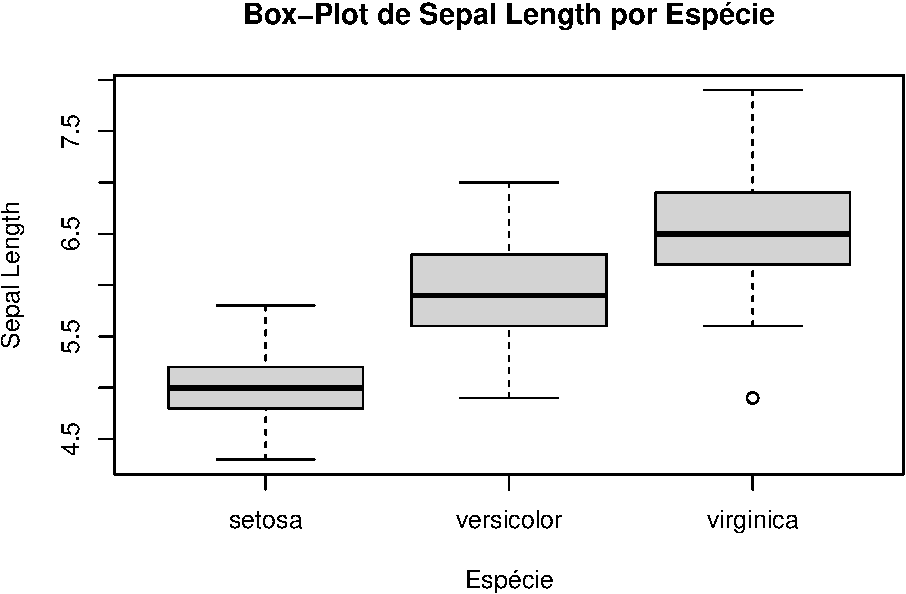
\includegraphics{introR_files/figure-latex/unnamed-chunk-180-1.pdf}

\section{Geração de números pseudoaleatórios}\label{gerauxe7uxe3o-de-nuxfameros-pseudoaleatuxf3rios}

\textbf{Números Aleatórios}

Números aleatórios são valores que são gerados de forma imprevisível e
não seguem nenhum padrão determinado. Em outras palavras, cada número em
uma sequência de números aleatórios é escolhido de maneira independente
dos outros, sem qualquer correlação entre eles. Na prática, os números
aleatórios são usados em diversas áreas, como criptografia, simulações,
estatísticas, jogos de azar, entre outros, onde é crucial que os números
não possam ser antecipados.

A verdadeira aleatoriedade é geralmente derivada de processos físicos
que são inerentemente imprevisíveis, como a radiação cósmica, ruído
térmico em circuitos eletrônicos, ou o decaimento radioativo. Em
computação, no entanto, obter números verdadeiramente aleatórios é
difícil e muitas vezes desnecessário.

\textbf{Números Pseudoaleatórios}

Números pseudoaleatórios, por outro lado, são números que são gerados
por algoritmos que produzem sequências que parecem aleatórias, mas são,
na verdade, determinadas por um valor inicial chamado semente (ou ``seed''
em inglês). Se o algoritmo é iniciado com a mesma semente, ele produzirá
exatamente a mesma sequência de números.

Embora sejam determinísticos, os números pseudoaleatórios são amplamente
utilizados porque podem ser gerados rapidamente e, para muitas
aplicações, eles são suficientemente aleatórios. A principal vantagem é
que, ao usar a mesma semente, é possível replicar experimentos ou
simulações, o que é útil em pesquisas e depurações.

Uma das aproximações mais comuns para gerar números pseudoaleatórios é o
método \emph{congruencial multiplicativo}:

\begin{itemize}
\item
  Considere um valor inicial \(x_0\), chamado semente;
\item
  Recursivamente calcule os valores sucessivos \(x_{n}\), \(n\geq 1\),
  usando: \[x_{n} = ax_{n-1} \, \text{mod}\, m,\] onde \(a\) e \(m\) são
  inteiros positivos dados. Ou seja, \(x_{n}\) é o resto da divisão
  inteira de \(ax_{n-1}\) por m;
\item
  A quantidade \(x_{n}/m\) é chamada um número pseudoaleatório, ou seja,
  é uma aproximação para o valor de uma variável aleatória uniforme.
\end{itemize}

As constantes \(a\) e \(m\) a serem escolhidas devem satisfazer três
critérios:

\begin{itemize}
\item
  Para qualquer semente inicial, a sequência resultante deve ter a
  ``aparência'' de uma sequência de variáveis aleatórias uniformes
  \((0,1)\) independentes.
\item
  Para qualquer semente inicial, o número de variáveis que podem ser
  geradas antes da repetição ocorrer deve ser grande.
\item
  Os valores podem ser calculados eficientemente em um computador.
\end{itemize}

\section{\texorpdfstring{A função \texttt{sample()}}{A função sample()}}\label{a-funuxe7uxe3o-sample}

A função \texttt{sample()} em R é utilizada para gerar uma amostra aleatória a
partir de um conjunto de dados ou uma sequência de números. Ela é
extremamente flexível, permitindo que você defina o tamanho da amostra,
se a amostragem é feita com ou sem reposição, e também se os elementos
têm probabilidades diferentes de serem selecionados.

\begin{Shaded}
\begin{Highlighting}[]
\CommentTok{\# Sintaxe}

\FunctionTok{sample}\NormalTok{(x, size, }\AttributeTok{replace =} \ConstantTok{FALSE}\NormalTok{, }\AttributeTok{prob =} \ConstantTok{NULL}\NormalTok{)}
\end{Highlighting}
\end{Shaded}

\begin{itemize}
\item
  \textbf{x}: Vetor de elementos a serem amostrados.
\item
  \textbf{size}: Tamanho da amostra.
\item
  \textbf{replace}: Indica se a amostragem é com reposição (\texttt{TRUE}) ou sem
  reposição (\texttt{FALSE}).
\item
  \textbf{prob}: Um vetor de probabilidades associadas a cada elemento em

  \begin{enumerate}
  \def\labelenumi{\alph{enumi}.}
  \setcounter{enumi}{23}
  \tightlist
  \item
  \end{enumerate}
\end{itemize}

\textbf{Exemplo 1}: Amostragem Simples sem Reposição.

\begin{Shaded}
\begin{Highlighting}[]
\CommentTok{\# Suponha que temos uma população de 1 a 10}
\NormalTok{pop }\OtherTok{\textless{}{-}} \DecValTok{1}\SpecialCharTok{:}\DecValTok{10}

\CommentTok{\# Queremos uma amostra de 5 elementos}
\NormalTok{amostra }\OtherTok{\textless{}{-}} \FunctionTok{sample}\NormalTok{(pop, }\AttributeTok{size =} \DecValTok{5}\NormalTok{, }\AttributeTok{replace =} \ConstantTok{FALSE}\NormalTok{)}
\FunctionTok{print}\NormalTok{(amostra)}
\DocumentationTok{\#\# [1]  5  2  4 10  8}
\end{Highlighting}
\end{Shaded}

\textbf{Exemplo 2}: Amostragem com Reposição.

\begin{Shaded}
\begin{Highlighting}[]
\CommentTok{\# Amostra com reposição}
\NormalTok{amostra\_repos }\OtherTok{\textless{}{-}} \FunctionTok{sample}\NormalTok{(pop, }\AttributeTok{size =} \DecValTok{5}\NormalTok{, }\AttributeTok{replace =} \ConstantTok{TRUE}\NormalTok{)}
\FunctionTok{print}\NormalTok{(amostra\_repos)}
\DocumentationTok{\#\# [1] 6 8 9 9 6}
\end{Highlighting}
\end{Shaded}

\textbf{Exemplo 3}: Amostragem com Probabilidades Diferentes.

\begin{Shaded}
\begin{Highlighting}[]
\CommentTok{\# Probabilidades associadas a cada elemento}
\NormalTok{prob }\OtherTok{\textless{}{-}} \FunctionTok{c}\NormalTok{(}\FloatTok{0.1}\NormalTok{, }\FloatTok{0.1}\NormalTok{, }\FloatTok{0.1}\NormalTok{, }\FloatTok{0.1}\NormalTok{, }\FloatTok{0.1}\NormalTok{, }\FloatTok{0.1}\NormalTok{, }\FloatTok{0.1}\NormalTok{, }\FloatTok{0.1}\NormalTok{, }\FloatTok{0.05}\NormalTok{, }\FloatTok{0.05}\NormalTok{)}

\CommentTok{\# Amostra com probabilidades diferentes}
\NormalTok{amostra\_prob }\OtherTok{\textless{}{-}} \FunctionTok{sample}\NormalTok{(pop, }\AttributeTok{size =} \DecValTok{5}\NormalTok{, }\AttributeTok{prob =}\NormalTok{ prob)}
\FunctionTok{print}\NormalTok{(amostra\_prob)}
\DocumentationTok{\#\# [1] 2 4 6 5 3}
\end{Highlighting}
\end{Shaded}

\section{Exercícios}\label{exercuxedcios-17}

\textbf{1.} Crie um vetor com os números de 1 a 20. Utilize a função \texttt{sample()}
para selecionar uma amostra aleatória de 5 elementos desse vetor. A
amostragem deve ser feita sem reposição.

\textbf{2.} Suponha que você tem uma população representada pelos números de 1
a 10. Utilize a função \texttt{sample()} para selecionar uma amostra de 10
elementos com reposição.

\textbf{3.} Crie um vetor com as letras A, B, C, D, E. Aplique a função
\texttt{sample()} para selecionar uma amostra de 3 letras, onde a
probabilidade de cada letra ser selecionada é dada pelo vetor
\texttt{c(0.1,\ 0.2,\ 0.3,\ 0.25,\ 0.15)}.

\textbf{4.} Crie um vetor com os números de 1 a 10. Utilize a função \texttt{sample()}
para reordenar aleatoriamente os elementos desse vetor.

\textbf{5.} Crie um vetor com os nomes de cinco frutas: ``Maçã'', ``Banana'',
``Laranja'', ``Uva'', ``Pera''. Utilizando a função \texttt{sample()}, selecione
aleatoriamente uma fruta desse vetor. Em seguida, selecione uma
amostra de 3 frutas.

\textbf{6.} Você é responsável por realizar um teste de qualidade em uma
fábrica. Há 1000 produtos fabricados, numerados de 1 a 1000.
Selecione uma amostra aleatória de 50 produtos para inspeção,
garantindo que não haja reposição na seleção.

\textbf{7.} Simule o lançamento de dois dados justos 10000 vezes e registre as
somas das faces resultantes. Utilize a função \texttt{sample()} para
realizar a simulação. Em seguida, crie um histograma das somas
obtidas.

\textbf{8.} Você possui um vetor de 200 estudantes classificados em três turmas:
A, B, e C. As turmas têm tamanhos diferentes (50, 100, e 50 alunos,
respectivamente). Usando \texttt{sample()}, selecione uma amostra de 20
alunos, mantendo a proporção original das turmas.

\textbf{9.} Um cartão de Bingo contém 24 números aleatórios entre 1 e 75
(excluindo o número central ``free''). Crie 5 cartões de Bingo únicos
usando a função \texttt{sample()}.

\textbf{10.} Em um estudo clínico, 30 pacientes devem ser randomizados em dois
grupos: tratamento e controle. O grupo de tratamento deve conter 20
pacientes e o grupo de controle 10. Usando \texttt{sample()}, faça a
randomização dos pacientes. Dica: use a função \texttt{setdiff()}.

\chapter{Método da transformada inversa}\label{muxe9todo-da-transformada-inversa}

\section{Variável aleatória discreta}\label{variuxe1vel-aleatuxf3ria-discreta}

Suponha que queremos gerar o valor de uma variável aleatória discreta \(X\) com função massa de probabilidade \(P(X = x_{i}) = p_{i}\), \(i=0,1,\ldots\), \(\sum_{i}p_{i}=1\). Para isso, basta gerar um número aleatório \(U \sim U(0,1)\) e considerar:
\[X = \begin{cases}
x_{0},& \quad \text{se} \quad U<p_{0} \\
x_{1},& \quad \text{se} \quad p_{0}\leq U <p_{0}+p_{1}\\
\vdots& \\
x_{i},& \quad \text{se} \quad \sum_{j=0}^{i-1}p_{j}\leq U < \sum_{j=0}^{i}p_{j} \\
\vdots
\end{cases}\]

Como, para \(0<a<b<1\), \(P(a\leq U<b)=b-a\), temos que \[P(X=x_{i}) = P\left( \sum_{j=0}^{i-1}p_{j} \leq U < \sum_{j=0}^{i}p_{j} \right) = p_{i.}\]

Se os \(x_{i}\), \(i\geq 0\), estão ordenados \(x_{0}<x_{1}<\cdots\) e se denotarmos por \(F\) a função de distribuição de \(X\), então \(F(x_{k})=\sum_{i=0}^{k}p_{i}\) e assim \[X = x_{i} \quad \text{se} \quad F(x_{i-1})\leq U < F(x_{i})\]

Em outras palavras, depois de gerar um número aleatório \(U\) nós determinamos o valor de \(X\) encontrando o intervalo \([F(x_{i-1}),F(x_{i})]\) no qual \(U\) pertence (ou, equivalentemente, encontrando a inversa de \(F(U)\)).

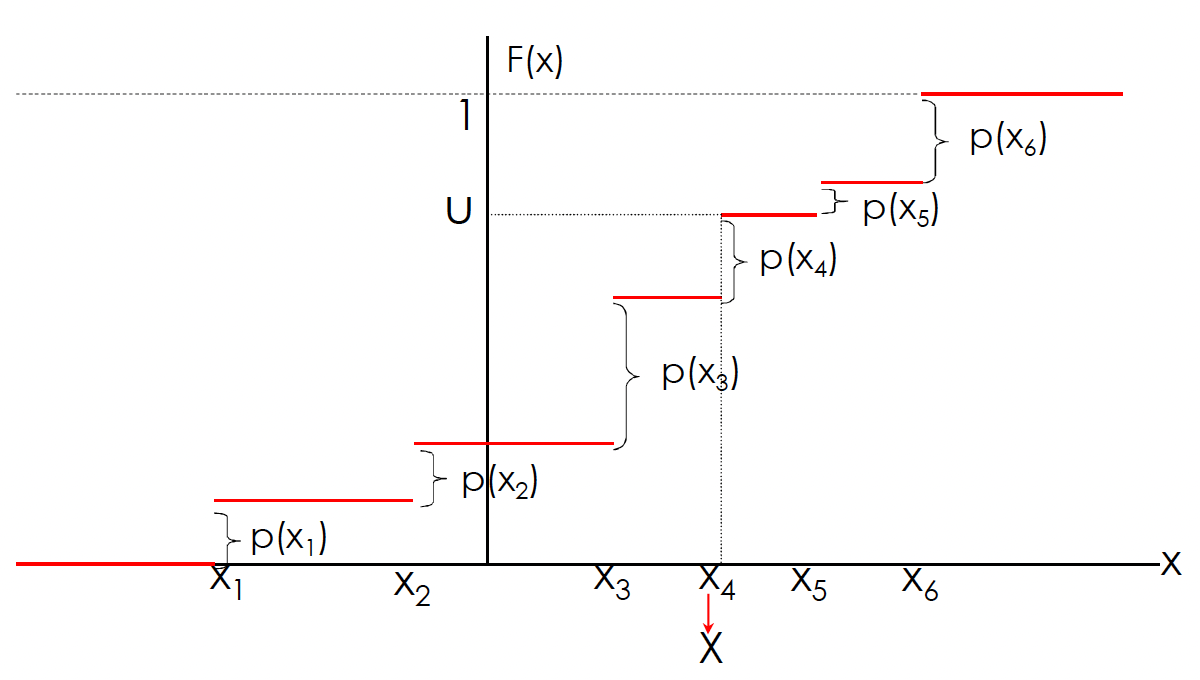
\includegraphics{docs/transf_inversa1.png}
\textbf{Exemplo 1}: Seja \(X\) uma variável aleatória discreta tal que \(p_{1}=0.20\), \(p_{2}=0.15\), \(p_{3}=0.25\), \(p_{4}=0.40\) onde \(p_{j}=P(X=j)\). Gere 1000 valores dessa variável aleatória.

Para a variável aleatória \(X\), a função de distribuição acumulada é dada pela soma cumulativa das probabilidades:

\[
F(x) = 
\begin{cases} 
0, & \text{se } x < 1 \\
p_1, & \text{se } 1 \leq x < 2 \\
p_1 + p_2, & \text{se } 2 \leq x < 3 \\
p_1 + p_2 + p_3, & \text{se } 3 \leq x < 4 \\
1, & \text{se } x \geq 4 
\end{cases}
\]

Com os valores fornecidos:

\[
F(x) = 
\begin{cases} 
0, & \text{se } x < 1 \\
0.20, & \text{se } 1 \leq x < 2 \\
0.35, & \text{se } 2 \leq x < 3 \\
0.60, & \text{se } 3 \leq x < 4 \\
1, & \text{se } x \geq 4 
\end{cases}
\]

Gerar um número aleatório uniforme \(U\) no intervalo {[}0,1{]}. Para determinar o valor de \(X\) correspondente a \(U\):

\begin{itemize}
\tightlist
\item
  Se \(U <0.20\), então \(X=1\)
\item
  Se \(0.20 \leq U < 0.35\), então \(X=2\)
\item
  Se \(0.35\leq U < 0.60\), então \(X=3\)
\item
  Se \(0.60 \leq U \leq 1\), então \(X=4\)
\end{itemize}

\textbf{Exemplo 2}: Seja \(X\) uma variável aleatória discreta assumindo os valores: \(1,2,\ldots,10\) com probabilidade \(1/10\) para \(x=1,2,\ldots,10\). Gerar 5000 valores dessa variável aleatória. Representar graficamente e determinar: média, desvio padrão e mediana.

\begin{Shaded}
\begin{Highlighting}[]
\NormalTok{gerar\_va\_inversa }\OtherTok{\textless{}{-}} \ControlFlowTok{function}\NormalTok{()\{}
  \CommentTok{\# Gerar número aleatório entre 0 e 1}
\NormalTok{  u }\OtherTok{\textless{}{-}} \FunctionTok{runif}\NormalTok{(}\DecValTok{1}\NormalTok{,}\DecValTok{0}\NormalTok{,}\DecValTok{1}\NormalTok{)}
\NormalTok{  p }\OtherTok{\textless{}{-}} \DecValTok{1}\SpecialCharTok{/}\DecValTok{10} \CommentTok{\# primeira probabilidade P(X=1)}
\NormalTok{  F }\OtherTok{\textless{}{-}}\NormalTok{ p }\CommentTok{\# inicializar a função de distribuição acumulada}
\NormalTok{  X }\OtherTok{\textless{}{-}} \DecValTok{1} \CommentTok{\# inicializar o valor da va X}
  
  \ControlFlowTok{while}\NormalTok{(u }\SpecialCharTok{\textgreater{}}\NormalTok{ F)\{}
\NormalTok{    X }\OtherTok{\textless{}{-}}\NormalTok{ X}\SpecialCharTok{+}\DecValTok{1}
\NormalTok{    F }\OtherTok{\textless{}{-}}\NormalTok{ F}\SpecialCharTok{+}\NormalTok{p}
\NormalTok{  \}}
  \FunctionTok{return}\NormalTok{(X)}
\NormalTok{\}}
\NormalTok{valores }\OtherTok{\textless{}{-}} \FunctionTok{replicate}\NormalTok{(}\DecValTok{5000}\NormalTok{,}\FunctionTok{gerar\_va\_inversa}\NormalTok{())}
\FunctionTok{hist}\NormalTok{(valores, }\AttributeTok{freq =} \ConstantTok{FALSE}\NormalTok{)}
\end{Highlighting}
\end{Shaded}

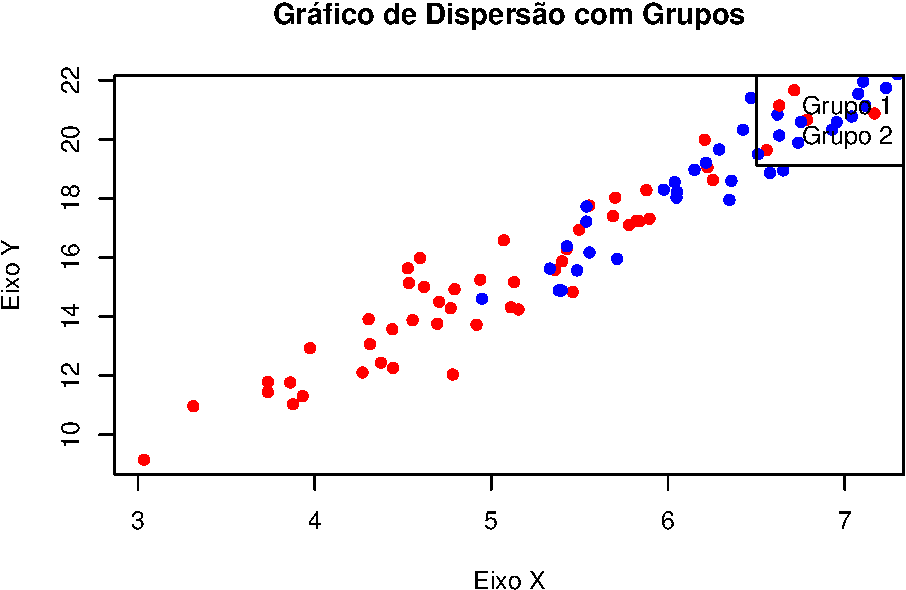
\includegraphics{introR_files/figure-latex/unnamed-chunk-185-1.pdf}

\begin{Shaded}
\begin{Highlighting}[]
\FunctionTok{mean}\NormalTok{(valores)}
\end{Highlighting}
\end{Shaded}

\begin{verbatim}
## [1] 5.5388
\end{verbatim}

\begin{Shaded}
\begin{Highlighting}[]
\FunctionTok{sd}\NormalTok{(valores)}
\end{Highlighting}
\end{Shaded}

\begin{verbatim}
## [1] 2.878985
\end{verbatim}

\begin{Shaded}
\begin{Highlighting}[]
\FunctionTok{median}\NormalTok{(valores)}
\end{Highlighting}
\end{Shaded}

\begin{verbatim}
## [1] 6
\end{verbatim}

\textbf{Exemplo 3}: Geração de uma variável aleatória com distribuição de Bernoulli. A variável aleatória \(X\) é de Bernoulli com parâmetro \(p\) se \[P(X = x) = \begin{cases} 1-p,& \quad \text{se} \quad x=0\\
p,& \quad \text{se} \quad x=1 \end{cases}\] Para gerar uma Bernoulli(p) podemos usar o seguinte algoritmo que é equivalente ao método da transformada inversa

\begin{enumerate}
\def\labelenumi{\arabic{enumi}.}
\tightlist
\item
  Gerar um número aleatório \(U\);
\item
  Se \(U \leq p\) então \(X=1\) senão \(X=0\).
\end{enumerate}

\begin{Shaded}
\begin{Highlighting}[]
\CommentTok{\# Gerando uma variável aleatória com distribuição de Bernoulli(p)}
\NormalTok{gerar\_bernoulli\_inversa }\OtherTok{\textless{}{-}} \ControlFlowTok{function}\NormalTok{(p)\{}
\NormalTok{  U }\OtherTok{\textless{}{-}} \FunctionTok{runif}\NormalTok{(}\DecValTok{1}\NormalTok{)}
  \ControlFlowTok{if}\NormalTok{ (U }\SpecialCharTok{\textless{}=}\NormalTok{ p)\{}
\NormalTok{    X }\OtherTok{\textless{}{-}} \DecValTok{1}
\NormalTok{  \} }\ControlFlowTok{else}\NormalTok{ \{}
\NormalTok{    X }\OtherTok{\textless{}{-}} \DecValTok{0}
\NormalTok{  \}}
  \FunctionTok{return}\NormalTok{(X)}
\NormalTok{\}}

\NormalTok{valores }\OtherTok{\textless{}{-}} \FunctionTok{replicate}\NormalTok{(}\DecValTok{100}\NormalTok{,}\FunctionTok{gerar\_bernoulli\_inversa}\NormalTok{(}\FloatTok{0.8}\NormalTok{))}
\FunctionTok{sum}\NormalTok{(valores)}\SpecialCharTok{/}\DecValTok{100}
\end{Highlighting}
\end{Shaded}

\begin{verbatim}
## [1] 0.73
\end{verbatim}

\textbf{Exemplo 4}: Gerar uma variável aleatória com distribuição Binomial(n,p). Aqui podemos usar o facto de que se \(X_{1},X_{2},\ldots,X_{n}\) são Bernoullis i.i.d., então \[X = X_{1}+X_{2}+\ldots+X_{n}\] é uma Binomial(n,p).

\begin{Shaded}
\begin{Highlighting}[]
\CommentTok{\# Gerando uma variável aleatória com distribuição Binomial(n,p)}

\NormalTok{gerar\_binomial\_inversa }\OtherTok{\textless{}{-}} \ControlFlowTok{function}\NormalTok{(n,p)\{}
\NormalTok{  X }\OtherTok{\textless{}{-}} \FunctionTok{sum}\NormalTok{(}\FunctionTok{replicate}\NormalTok{(n,}\FunctionTok{gerar\_bernoulli\_inversa}\NormalTok{(p)))}
  \FunctionTok{return}\NormalTok{(X)}
\NormalTok{\}}

\NormalTok{valores }\OtherTok{\textless{}{-}} \FunctionTok{replicate}\NormalTok{(}\DecValTok{10000}\NormalTok{,}\FunctionTok{gerar\_binomial\_inversa}\NormalTok{(}\DecValTok{10}\NormalTok{,}\FloatTok{0.5}\NormalTok{))}
\FunctionTok{hist}\NormalTok{(valores, }\AttributeTok{freq =} \ConstantTok{FALSE}\NormalTok{)}
\FunctionTok{points}\NormalTok{(}\DecValTok{1}\SpecialCharTok{:}\DecValTok{10}\NormalTok{, }\FunctionTok{dbinom}\NormalTok{(}\DecValTok{1}\SpecialCharTok{:}\DecValTok{10}\NormalTok{,}\DecValTok{10}\NormalTok{,}\FloatTok{0.5}\NormalTok{))}
\end{Highlighting}
\end{Shaded}

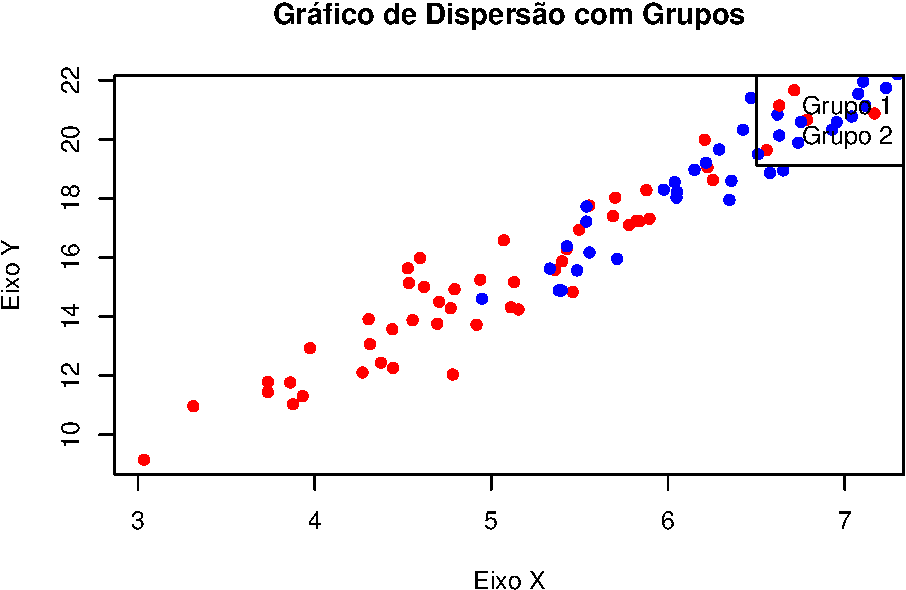
\includegraphics{introR_files/figure-latex/unnamed-chunk-187-1.pdf}

\textbf{Exemplo 5}: Geração de uma variável aleatória com distribuição Geométrica(p). Seja \(X\sim Geometrica(p)\). Lembre que \[P(X=x)=p(1-p)^{x-1}\] e que \[F(x) = P(X\leq x) = \begin{cases} 0,& \quad \text{se} \quad x<1 \\
1-(1-p)^x,& \quad \text{se} \quad x\geq 1\end{cases}\]
O seguinte algoritmo é equivalente ao método da transformada inversa:

\begin{enumerate}
\def\labelenumi{\arabic{enumi}.}
\item
  Gerar um número aleatório \(U\);
\item
  Fazer \(X = \lfloor ln(U)/ln(1-p)\rfloor\)
\end{enumerate}

onde \(\lfloor  \rfloor =\) maior inteiro.

\begin{Shaded}
\begin{Highlighting}[]
\CommentTok{\# Gerar uma variável aleatória com distribuição Geométrica(p)}

\NormalTok{gerar\_geometrica\_inversa }\OtherTok{\textless{}{-}} \ControlFlowTok{function}\NormalTok{(p)\{}
\NormalTok{  U }\OtherTok{\textless{}{-}} \FunctionTok{runif}\NormalTok{(}\DecValTok{1}\NormalTok{)}
\NormalTok{  X }\OtherTok{\textless{}{-}} \FunctionTok{round}\NormalTok{(}\FunctionTok{log}\NormalTok{(U)}\SpecialCharTok{/}\FunctionTok{log}\NormalTok{(}\DecValTok{1}\SpecialCharTok{{-}}\NormalTok{p))}
  \FunctionTok{return}\NormalTok{(X)}
\NormalTok{\}}

\NormalTok{valores }\OtherTok{\textless{}{-}} \FunctionTok{replicate}\NormalTok{(}\DecValTok{10000}\NormalTok{, }\FunctionTok{gerar\_geometrica\_inversa}\NormalTok{(}\FloatTok{0.5}\NormalTok{))}
\FunctionTok{hist}\NormalTok{(valores, }\AttributeTok{freq =} \ConstantTok{FALSE}\NormalTok{)}
\FunctionTok{points}\NormalTok{(}\DecValTok{1}\SpecialCharTok{:}\DecValTok{10}\NormalTok{, }\FunctionTok{dgeom}\NormalTok{(}\DecValTok{1}\SpecialCharTok{:}\DecValTok{10}\NormalTok{,}\FloatTok{0.5}\NormalTok{))}
\end{Highlighting}
\end{Shaded}

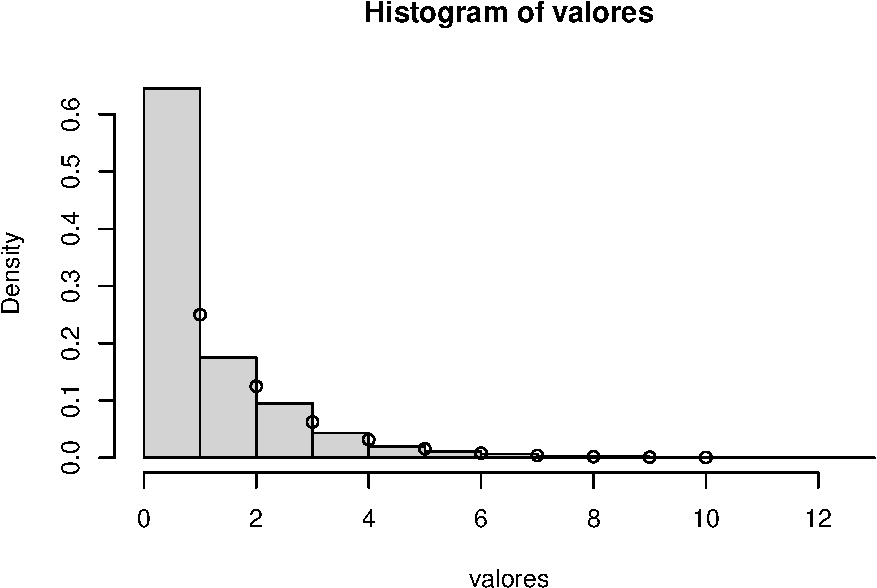
\includegraphics{introR_files/figure-latex/unnamed-chunk-188-1.pdf}

\textbf{Exemplo 6}: Geração de uma variável aleatória com distribuição de Poisson. A variável aleatória \(X\) é de Poisson com média \(\lambda\) se \[p_{i} = P(X = i) = \frac{e^{-\lambda}\lambda^i}{i!}, \quad i=0,1,\ldots\]

A chave para usar o método da transformada inversa para gerar uma tal variável aleatória é dada pela seguinte identidade: \[p_{i+1}=\frac{\lambda}{i+1}p_{i}, \quad i\geq 0.\]

Ao utilizar a recursão acima para calcular as probabilidades de Poisson quando elas são necessárias, o algoritmo da transformada inversa para gerar uma variável aleatória de Poisson com média \(\lambda\) pode ser expresso como segue.

\begin{Shaded}
\begin{Highlighting}[]
\CommentTok{\# Gerando uma va com distribuição de Poisson}

\NormalTok{lambda }\OtherTok{\textless{}{-}} \DecValTok{3}  \CommentTok{\# exemplo com lambda = 3}

\CommentTok{\# Função para gerar uma variável aleatória de Poisson usando o método da transformada inversa}
\NormalTok{gerar\_poisson\_inversa }\OtherTok{\textless{}{-}} \ControlFlowTok{function}\NormalTok{(lambda) \{}
\NormalTok{  U }\OtherTok{\textless{}{-}} \FunctionTok{runif}\NormalTok{(}\DecValTok{1}\NormalTok{)  }\CommentTok{\# Gerar um número aleatório uniforme entre 0 e 1}
\NormalTok{  p }\OtherTok{\textless{}{-}} \FunctionTok{exp}\NormalTok{(}\SpecialCharTok{{-}}\NormalTok{lambda)  }\CommentTok{\# Inicializar a primeira probabilidade P(X=0)}
\NormalTok{  F }\OtherTok{\textless{}{-}}\NormalTok{ p  }\CommentTok{\# Inicializar a função de distribuição acumulada (CDF)}
\NormalTok{  X }\OtherTok{\textless{}{-}} \DecValTok{0}  \CommentTok{\# Inicializar o valor da variável aleatória}
  
  \CommentTok{\# Acumular probabilidades até que a CDF exceda U}
  \ControlFlowTok{while}\NormalTok{ (U }\SpecialCharTok{\textgreater{}}\NormalTok{ F) \{}
\NormalTok{    X }\OtherTok{\textless{}{-}}\NormalTok{ X }\SpecialCharTok{+} \DecValTok{1}
\NormalTok{    p }\OtherTok{\textless{}{-}}\NormalTok{ p }\SpecialCharTok{*}\NormalTok{ lambda }\SpecialCharTok{/}\NormalTok{ X  }\CommentTok{\# Atualizar a probabilidade P(X=k)}
\NormalTok{    F }\OtherTok{\textless{}{-}}\NormalTok{ F }\SpecialCharTok{+}\NormalTok{ p  }\CommentTok{\# Atualizar a CDF}
\NormalTok{  \}}
  
  \FunctionTok{return}\NormalTok{(X)}
\NormalTok{\}}

\FunctionTok{hist}\NormalTok{(}\FunctionTok{replicate}\NormalTok{(}\DecValTok{10000}\NormalTok{,}\FunctionTok{gerar\_poisson\_inversa}\NormalTok{(}\DecValTok{3}\NormalTok{)),}\AttributeTok{freq =} \ConstantTok{FALSE}\NormalTok{)}
\FunctionTok{points}\NormalTok{(}\DecValTok{1}\SpecialCharTok{:}\DecValTok{10}\NormalTok{,}\FunctionTok{dpois}\NormalTok{(}\DecValTok{1}\SpecialCharTok{:}\DecValTok{10}\NormalTok{,}\DecValTok{3}\NormalTok{))}
\end{Highlighting}
\end{Shaded}

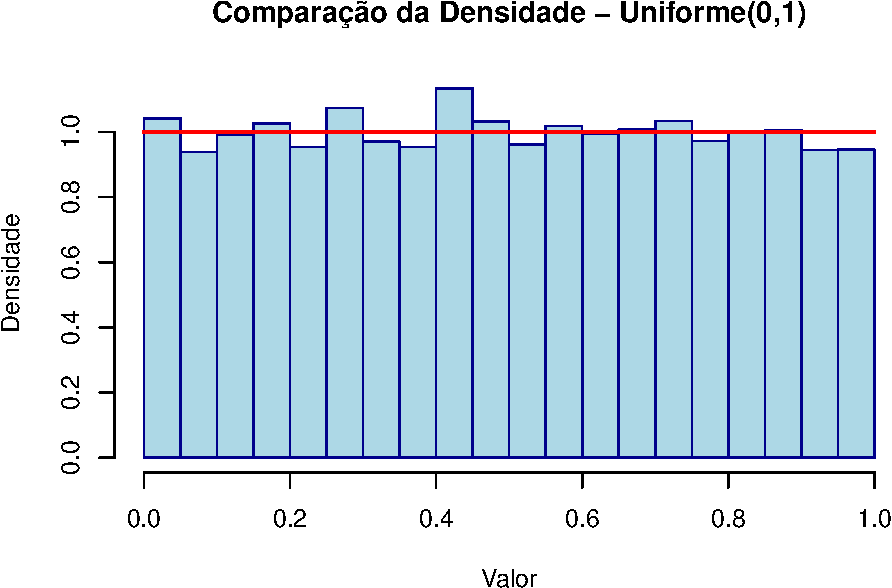
\includegraphics{introR_files/figure-latex/unnamed-chunk-189-1.pdf}

\section{Variável aleatória contínua}\label{variuxe1vel-aleatuxf3ria-contuxednua}

Uma variável aleatória \(X\) tem densidade \(f(x)=2x\), para \(0<x<1\), e 0, caso contrário. Suponha que queremos simular observações de \(X\). Nesta secção, apresentaremos um método simples e flexível para simulação de uma distribuição contínua.

\textbf{Proposição}: Suponha que \(X\) é uma variável aleatória com função de distribuição \(F\), onde \(F\) é invertível com função inversa \(F^{-1}\). Seja \(U\) uma variável aleatória uniforme \((0,1)\). Então a distribuição de \(F^{-1}(U)\) é igual a distribuição de \(X\), ou seja, a variável aleatória \(X\) definida por \(X=F^{-1}(U)\) tem distribuição \(F\).

A prova desta proposição é fácil e rápida. Precisamos mostrar que \(F^{-1}(U)\) tem a mesma distribuição que \(X\). Assim,

\begin{align*}
P(X \leq x) &= P(F^{-1}(U)\leq x) = P(FF^{-1}(U) \leq F(x)) \\
&= P(U \leq F(x)) = P(0\leq U \leq F(x)) \\
&= F(x)-0 \\
&= F(x).
\end{align*}

A última igualdade segue do facto de que \(U\sim U(0,1)\) e \(0\leq F(x) \leq 1\).

Essa proposição mostra que pode-se gerar uma variável aleatória \(X\) de uma função de distribuição contínua \(F\) gerando um número aleatório \(U\) e tomando \(X = F^{-1}(U)\).

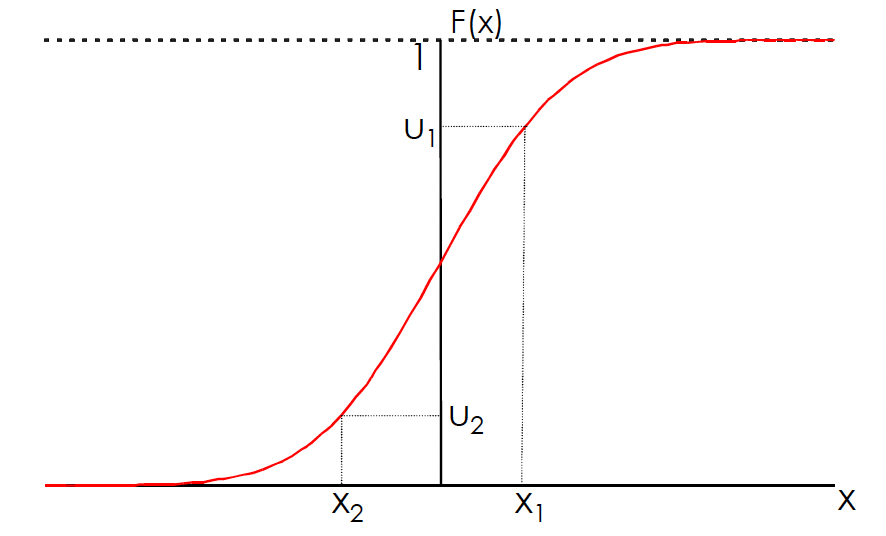
\includegraphics{docs/transf_inversa2.png}

\textbf{Exemplo 1}: Considere nossa varíavel aleatória \(X\) com densidade \(f(x)=2x\). A função de distribuição de \(X\) é \[F(x)=P(X\leq x)=\int_{0}^{x}2t\, dt = x^2, \quad \text{para} \quad 0<x<1.\]

A função \(F(x)=x^2\) é invertível no intervalo \((0,1)\) e \(F^{-1}(x)=\sqrt{x}\). O método da transformada inversa diz que se \(U\sim U(0,1)\), então \(F^{-1}(U)=\sqrt{U}\) tem a mesma distribuição que \(X\). Portanto para simular \(X\), basta gerar \(\sqrt{U}\).

\begin{Shaded}
\begin{Highlighting}[]
\NormalTok{n }\OtherTok{\textless{}{-}} \DecValTok{10000}
\FunctionTok{set.seed}\NormalTok{(}\DecValTok{123}\NormalTok{)}
\NormalTok{simlist }\OtherTok{\textless{}{-}} \FunctionTok{sqrt}\NormalTok{(}\FunctionTok{runif}\NormalTok{(n))}
\FunctionTok{hist}\NormalTok{(simlist, }\AttributeTok{prob=}\NormalTok{T, }\AttributeTok{main=}\StringTok{""}\NormalTok{, }\AttributeTok{xlab=}\StringTok{""}\NormalTok{)}
\FunctionTok{curve}\NormalTok{(}\DecValTok{2}\SpecialCharTok{*}\NormalTok{x, }\DecValTok{0}\NormalTok{,}\DecValTok{1}\NormalTok{, }\AttributeTok{add=}\NormalTok{T)}
\end{Highlighting}
\end{Shaded}

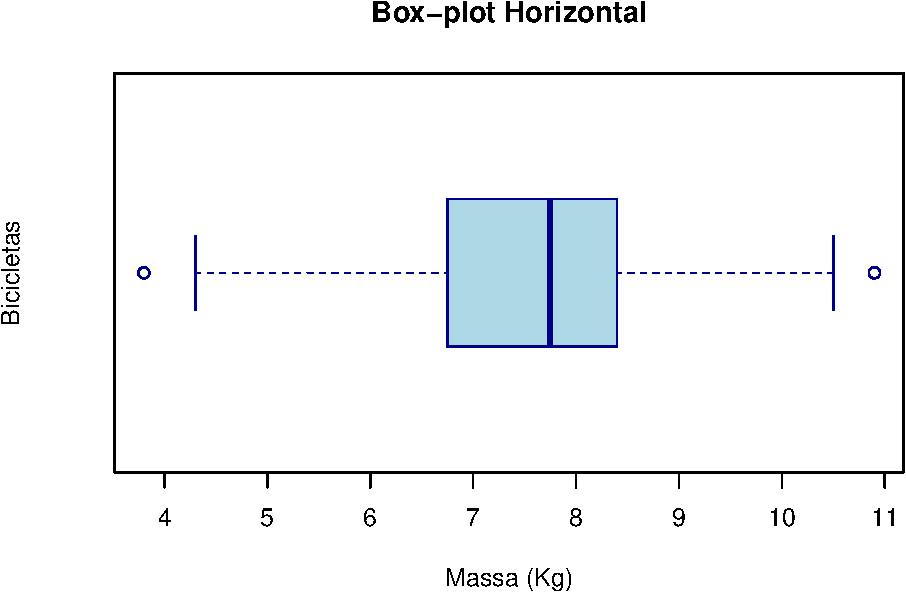
\includegraphics{introR_files/figure-latex/unnamed-chunk-190-1.pdf}

\textbf{Exemplo 2}: Geração de uma variável aleatória uniforme(a,b). A geração é feita através de \[X = a+(b-a)U.\]

\begin{Shaded}
\begin{Highlighting}[]
\CommentTok{\# Geração de uma va uniforme({-}2,2)}
\NormalTok{a }\OtherTok{\textless{}{-}} \SpecialCharTok{{-}}\DecValTok{2}
\NormalTok{b }\OtherTok{\textless{}{-}} \DecValTok{2}
\NormalTok{n }\OtherTok{\textless{}{-}} \DecValTok{10000}
\FunctionTok{set.seed}\NormalTok{(}\DecValTok{123}\NormalTok{)}
\NormalTok{simlist }\OtherTok{\textless{}{-}}\NormalTok{ a}\SpecialCharTok{+}\NormalTok{(b}\SpecialCharTok{{-}}\NormalTok{a)}\SpecialCharTok{*}\FunctionTok{runif}\NormalTok{(n)}
\FunctionTok{hist}\NormalTok{(simlist, }\AttributeTok{prob=}\NormalTok{T, }\AttributeTok{main=}\StringTok{""}\NormalTok{,}\AttributeTok{xlab=}\StringTok{""}\NormalTok{)}
\end{Highlighting}
\end{Shaded}

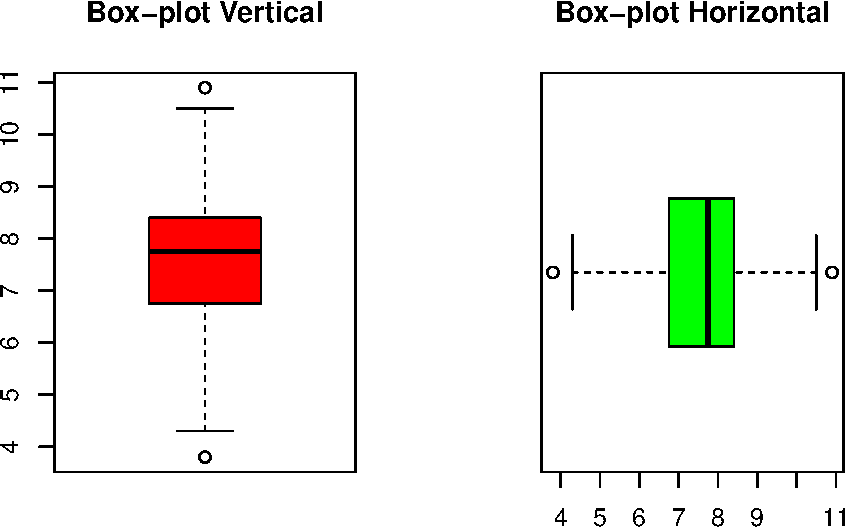
\includegraphics{introR_files/figure-latex/unnamed-chunk-191-1.pdf}

\textbf{Exemplo 3}: Geração de uma variável aleatória exponencial. Seja \(X\) uma variável aleatória exponencial com taxa 1, então sua função de distribuição é dada por \[F(x)=1-e^{x}.\]
Como \(0\leq F(x)\leq 1\), tomando \(F(x)=u\), onde \(u\sim U(0,1)\) tem-se: \[u=F(x)=1-e^{x}\] ou \[1-u=e^{-x}\] ou, aplicando o logaritmo \[x=-ln(1-u).\] Daí, pode-se gerar uma exponencial com parâmetro 1 gerando um número aleatório \(U\) e em seguida fazendo \[X = F^{-1}(U) = -ln(1-U).\] Uma pequena economia de tempo pode ser obtida notando que \(1-U\) também é uniforme em \((0,1)\) e assim, \(-ln(1-U)\) tem a mesma distribuição que \(-ln(U)\). Isto é, o logaritmo negativo de um número aleatório é exponencialmente distribuído com taxa 1.

Além disso, note que se \(X\) é uma exponencial com média 1, então para qualquer constante \(c\), \(cX\) é uma exponencial com média \(c\). Assim, uma variável aleatória exponencial \(X\) com taxa \(\lambda\) (média \(\frac{1}{\lambda}\)) pode ser gerada através da geração de um número aleatório \(U\) e fazendo \[X = -\frac{1}{\lambda}ln (U).\]

\begin{Shaded}
\begin{Highlighting}[]
\CommentTok{\# Definir a sequência de valores x}
\NormalTok{x }\OtherTok{\textless{}{-}} \FunctionTok{seq}\NormalTok{(}\DecValTok{0}\NormalTok{,}\DecValTok{3}\NormalTok{, }\AttributeTok{by =} \FloatTok{0.02}\NormalTok{)}

\CommentTok{\# Definir o parâmetro lambda da distribuição exponencial}
\NormalTok{lambda }\OtherTok{\textless{}{-}} \DecValTok{3}

\CommentTok{\# Número de simulação}
\NormalTok{n }\OtherTok{\textless{}{-}} \DecValTok{10000}

\CommentTok{\# Simular valores de uma distribuição exponencial}
\FunctionTok{set.seed}\NormalTok{(}\DecValTok{123}\NormalTok{)}
\NormalTok{simlist }\OtherTok{\textless{}{-}} \SpecialCharTok{{-}}\FunctionTok{log}\NormalTok{(}\FunctionTok{runif}\NormalTok{(n))}\SpecialCharTok{/}\NormalTok{lambda}

\CommentTok{\# Plotar o histograma da simulação com a densidade de probabilidade}
\FunctionTok{hist}\NormalTok{(simlist, }\AttributeTok{probability =} \ConstantTok{TRUE}\NormalTok{, }\AttributeTok{main =} \StringTok{"Comparação da Distribuição Exponencial Simulada e Teórica"}\NormalTok{,}
     \AttributeTok{xlab =} \StringTok{"Valores"}\NormalTok{, }\AttributeTok{ylab =} \StringTok{"Densidade"}\NormalTok{, }\AttributeTok{col =} \StringTok{"lightblue"}\NormalTok{, }\AttributeTok{border =} \StringTok{"black"}\NormalTok{)}

\CommentTok{\# Adicionar a curva de densidade teórica}
\FunctionTok{curve}\NormalTok{(}\FunctionTok{dexp}\NormalTok{(x, }\AttributeTok{rate =}\NormalTok{ lambda), }\AttributeTok{add =} \ConstantTok{TRUE}\NormalTok{, }\AttributeTok{col =} \StringTok{"red"}\NormalTok{, }\AttributeTok{lwd =} \DecValTok{2}\NormalTok{)}

\CommentTok{\# Adicionar uma legenda}
\FunctionTok{legend}\NormalTok{(}\StringTok{"topright"}\NormalTok{, }\AttributeTok{legend =} \FunctionTok{c}\NormalTok{(}\StringTok{"Simulação"}\NormalTok{, }\StringTok{"Teórica"}\NormalTok{), }\AttributeTok{col =} \FunctionTok{c}\NormalTok{(}\StringTok{"lightblue"}\NormalTok{, }\StringTok{"red"}\NormalTok{), }\AttributeTok{lwd =} \DecValTok{2}\NormalTok{, }\AttributeTok{fill =} \FunctionTok{c}\NormalTok{(}\StringTok{"lightblue"}\NormalTok{, }\ConstantTok{NA}\NormalTok{))}
\end{Highlighting}
\end{Shaded}

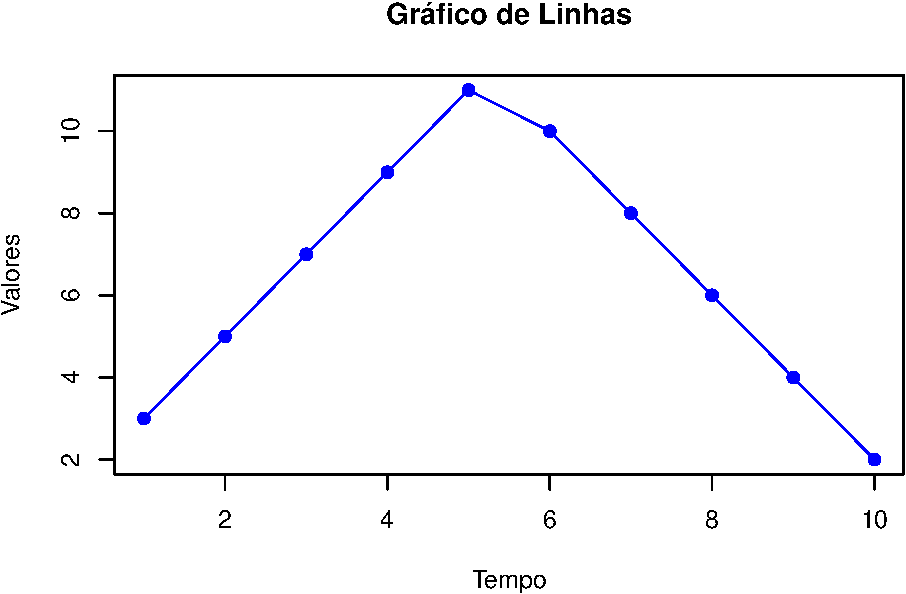
\includegraphics{introR_files/figure-latex/unnamed-chunk-192-1.pdf}

\textbf{Exercício}: Seja \(X\) uma variável aleatória com distribuição \(W(\alpha, \beta)\). Assim a fdp de \(X\) é
\[f(x) = \begin{cases}
\alpha \beta^{-\alpha} x^{\alpha -1} e^{-(x/\beta)^\alpha},& \quad \text{se} \quad x>0 \\
0,& \quad \text{se} \quad x\leq 0
\end{cases}\]

A função de distribuição de \(X\) é:
\[F(x) = \int_{0}^{x}f(u)\, du = \begin{cases}
1-e^{-(x/\beta)^\alpha},& \quad \text{se} \quad x>0\\
0,& \quad \text{se} \quad x\leq 0
\end{cases}\]

Mostre que \(X = \beta[-ln(U)]^{1/\alpha}\). Gere 10000 valores de uma \(W(2,3)\). Represente graficamente a distribuição.

\chapter{Método da aceitação-rejeição}\label{muxe9todo-da-aceitauxe7uxe3o-rejeiuxe7uxe3o}

\chapter{Distribuições univariadas no R}\label{distribuiuxe7uxf5es-univariadas-no-r}

No R temos acesso as mais comuns distribuições univariadas. Todas as
funções tem as seguintes formas:

\begin{longtable}[]{@{}
  >{\raggedright\arraybackslash}p{(\columnwidth - 2\tabcolsep) * \real{0.3611}}
  >{\raggedright\arraybackslash}p{(\columnwidth - 2\tabcolsep) * \real{0.6389}}@{}}
\toprule\noalign{}
\begin{minipage}[b]{\linewidth}\raggedright
\textbf{Função}
\end{minipage} & \begin{minipage}[b]{\linewidth}\raggedright
\textbf{Descrição}
\end{minipage} \\
\midrule\noalign{}
\endhead
\bottomrule\noalign{}
\endlastfoot
\textbf{p}nome( \ldots) & função de distribuição \\
\textbf{d}nome( \ldots) & função de probabilidade ou densidade de probabilidade \\
\textbf{q}nome( \ldots) & inversa da função de distribuição \\
\textbf{r}nome( \ldots) & geração de números aleatórios com a distribuição especificada \\
\end{longtable}

o \textbf{nome} é uma abreviatura do nome usual da distribuição (\texttt{binom},
\texttt{geom}, \texttt{pois}, \texttt{unif}, \texttt{exp}, \texttt{norm}, \ldots).

\textbf{Exempo 1}: Simule o lançamento de três moedas honestas e a contagem do número de caras X.

\textbf{(a)} Use a sua simulação para estimar \(P(X=1)\) e \(E(X)\).

\textbf{(b)} Modifique a alínea anterior para permitir uma moeda viciada onde \(P(cara)=3/4\).

\begin{Shaded}
\begin{Highlighting}[]
\FunctionTok{set.seed}\NormalTok{(}\DecValTok{123}\NormalTok{)}
\NormalTok{n }\OtherTok{\textless{}{-}} \DecValTok{10000}
\NormalTok{sim1 }\OtherTok{\textless{}{-}} \FunctionTok{numeric}\NormalTok{(n)}
\NormalTok{sim2 }\OtherTok{\textless{}{-}} \FunctionTok{numeric}\NormalTok{(n)}
\ControlFlowTok{for}\NormalTok{ (i }\ControlFlowTok{in} \DecValTok{1}\SpecialCharTok{:}\NormalTok{n) \{}
\NormalTok{  moedas }\OtherTok{\textless{}{-}} \FunctionTok{sample}\NormalTok{(}\DecValTok{0}\SpecialCharTok{:}\DecValTok{1}\NormalTok{,}\DecValTok{3}\NormalTok{,}\AttributeTok{replace=}\NormalTok{T)}
\NormalTok{  sim1[i] }\OtherTok{\textless{}{-}} \ControlFlowTok{if}\NormalTok{ (}\FunctionTok{sum}\NormalTok{(moedas)}\SpecialCharTok{==}\DecValTok{1}\NormalTok{) }\DecValTok{1} \ControlFlowTok{else} \DecValTok{0}
\NormalTok{  sim2[i] }\OtherTok{\textless{}{-}} \FunctionTok{sum}\NormalTok{(moedas)}
\NormalTok{\}}
\CommentTok{\# P(X=1)}
\FunctionTok{mean}\NormalTok{(sim1)}
\end{Highlighting}
\end{Shaded}

\begin{verbatim}
## [1] 0.3821
\end{verbatim}

\begin{Shaded}
\begin{Highlighting}[]
\CommentTok{\# E(X)}
\FunctionTok{mean}\NormalTok{(sim2)}
\end{Highlighting}
\end{Shaded}

\begin{verbatim}
## [1] 1.4928
\end{verbatim}

\begin{Shaded}
\begin{Highlighting}[]
\FunctionTok{set.seed}\NormalTok{(}\DecValTok{123}\NormalTok{)}
\NormalTok{n }\OtherTok{\textless{}{-}} \DecValTok{10000}
\NormalTok{sim1 }\OtherTok{\textless{}{-}} \FunctionTok{numeric}\NormalTok{(n)}
\NormalTok{sim2 }\OtherTok{\textless{}{-}} \FunctionTok{numeric}\NormalTok{(n)}
\ControlFlowTok{for}\NormalTok{ (i }\ControlFlowTok{in} \DecValTok{1}\SpecialCharTok{:}\NormalTok{n) \{}
\NormalTok{  moedas }\OtherTok{\textless{}{-}} \FunctionTok{sample}\NormalTok{(}\FunctionTok{c}\NormalTok{(}\DecValTok{0}\NormalTok{,}\DecValTok{1}\NormalTok{),}\DecValTok{3}\NormalTok{,}\AttributeTok{prob=}\FunctionTok{c}\NormalTok{(}\DecValTok{1}\SpecialCharTok{/}\DecValTok{4}\NormalTok{,}\DecValTok{3}\SpecialCharTok{/}\DecValTok{4}\NormalTok{),}\AttributeTok{replace=}\NormalTok{T)}
\NormalTok{  sim1[i] }\OtherTok{\textless{}{-}} \ControlFlowTok{if}\NormalTok{ (}\FunctionTok{sum}\NormalTok{(moedas)}\SpecialCharTok{==}\DecValTok{1}\NormalTok{) }\DecValTok{1} \ControlFlowTok{else} \DecValTok{0}
\NormalTok{  sim2[i] }\OtherTok{\textless{}{-}} \FunctionTok{sum}\NormalTok{(moedas)}
\NormalTok{\}}
\CommentTok{\# P(X=1)}
\FunctionTok{mean}\NormalTok{(sim1)}
\end{Highlighting}
\end{Shaded}

\begin{verbatim}
## [1] 0.1384
\end{verbatim}

\begin{Shaded}
\begin{Highlighting}[]
\CommentTok{\# E(X)}
\FunctionTok{mean}\NormalTok{(sim2)}
\end{Highlighting}
\end{Shaded}

\begin{verbatim}
## [1] 2.2503
\end{verbatim}

Sabemos também que \(X-\) número de caras no lançamneto de três moedas honestas tem distribuição \(Binomial(n=3,p=0.5)\). Assim, podemos resolver a questão da seguinte maneira

\begin{Shaded}
\begin{Highlighting}[]
\FunctionTok{set.seed}\NormalTok{(}\DecValTok{123}\NormalTok{)}
\NormalTok{valores }\OtherTok{\textless{}{-}} \FunctionTok{rbinom}\NormalTok{(}\DecValTok{10000}\NormalTok{,}\DecValTok{3}\NormalTok{,}\FloatTok{0.5}\NormalTok{)}
\CommentTok{\# P(X=1)}
\FunctionTok{sum}\NormalTok{(valores }\SpecialCharTok{==} \DecValTok{1}\NormalTok{)}\SpecialCharTok{/}\FunctionTok{length}\NormalTok{(valores)}
\end{Highlighting}
\end{Shaded}

\begin{verbatim}
## [1] 0.383
\end{verbatim}

\begin{Shaded}
\begin{Highlighting}[]
\CommentTok{\# E(X)}
\FunctionTok{sum}\NormalTok{(valores)}\SpecialCharTok{/}\FunctionTok{length}\NormalTok{(valores)}
\end{Highlighting}
\end{Shaded}

\begin{verbatim}
## [1] 1.4897
\end{verbatim}

\begin{Shaded}
\begin{Highlighting}[]
\FunctionTok{mean}\NormalTok{(valores)}
\end{Highlighting}
\end{Shaded}

\begin{verbatim}
## [1] 1.4897
\end{verbatim}

No segundo caso teremos \(X \sim Binomial(n=3,p=3/4)\).

\begin{Shaded}
\begin{Highlighting}[]
\FunctionTok{set.seed}\NormalTok{(}\DecValTok{123}\NormalTok{)}
\NormalTok{valores }\OtherTok{\textless{}{-}} \FunctionTok{rbinom}\NormalTok{(}\DecValTok{10000}\NormalTok{,}\DecValTok{3}\NormalTok{,}\DecValTok{3}\SpecialCharTok{/}\DecValTok{4}\NormalTok{)}
\CommentTok{\# P(X=1)}
\FunctionTok{sum}\NormalTok{(valores }\SpecialCharTok{==} \DecValTok{1}\NormalTok{)}\SpecialCharTok{/}\FunctionTok{length}\NormalTok{(valores)}
\end{Highlighting}
\end{Shaded}

\begin{verbatim}
## [1] 0.1365
\end{verbatim}

\begin{Shaded}
\begin{Highlighting}[]
\CommentTok{\# E(X)}
\FunctionTok{sum}\NormalTok{(valores)}\SpecialCharTok{/}\FunctionTok{length}\NormalTok{(valores)}
\end{Highlighting}
\end{Shaded}

\begin{verbatim}
## [1] 2.2558
\end{verbatim}

\begin{Shaded}
\begin{Highlighting}[]
\FunctionTok{mean}\NormalTok{(valores)}
\end{Highlighting}
\end{Shaded}

\begin{verbatim}
## [1] 2.2558
\end{verbatim}

\textbf{Exemplo 2}: O tempo até a chegada de um autocarro tem uma distribuição exponencial com média de 30 minutos.

\textbf{(a)} Use o comando \texttt{rexp()} para simular a probabilidade do autocarro chegar nos primeiros 20 minutos.

\textbf{(b)} Use o comando \texttt{pexp()} para comparar com a probabilidade exata.

\begin{Shaded}
\begin{Highlighting}[]
\FunctionTok{set.seed}\NormalTok{(}\DecValTok{123}\NormalTok{)}
\NormalTok{valores }\OtherTok{\textless{}{-}} \FunctionTok{rexp}\NormalTok{(}\DecValTok{10000}\NormalTok{, }\DecValTok{1}\SpecialCharTok{/}\DecValTok{30}\NormalTok{)}
\CommentTok{\# Probabilidade P(X \textless{}=20)}
\FunctionTok{sum}\NormalTok{( valores }\SpecialCharTok{\textless{}} \DecValTok{20}\NormalTok{)}\SpecialCharTok{/}\FunctionTok{length}\NormalTok{(valores)}
\end{Highlighting}
\end{Shaded}

\begin{verbatim}
## [1] 0.4832
\end{verbatim}

\begin{Shaded}
\begin{Highlighting}[]
\CommentTok{\# Probabilidade exata}
\FunctionTok{pexp}\NormalTok{(}\DecValTok{20}\NormalTok{, }\DecValTok{1}\SpecialCharTok{/}\DecValTok{30}\NormalTok{)}
\end{Highlighting}
\end{Shaded}

\begin{verbatim}
## [1] 0.4865829
\end{verbatim}

\textbf{Exemplo 3}: As cartas são retiradas de um baralho padrão, com reposição, até que um ás apareça. Simule a média e a variância do número de cartas necessárias.

\begin{Shaded}
\begin{Highlighting}[]
\FunctionTok{set.seed}\NormalTok{(}\DecValTok{123}\NormalTok{)}
\NormalTok{n }\OtherTok{\textless{}{-}} \DecValTok{10000}
\CommentTok{\# Denote os ases por 1,2,3,4 }
\NormalTok{simlist }\OtherTok{\textless{}{-}} \FunctionTok{numeric}\NormalTok{(n)}

\ControlFlowTok{for}\NormalTok{ (i }\ControlFlowTok{in} \DecValTok{1}\SpecialCharTok{:}\NormalTok{n) \{}
\NormalTok{  ct }\OtherTok{\textless{}{-}} \DecValTok{0}
\NormalTok{  as }\OtherTok{\textless{}{-}} \DecValTok{0}
  \ControlFlowTok{while}\NormalTok{ (as }\SpecialCharTok{==} \DecValTok{0}\NormalTok{) \{}
\NormalTok{    carta }\OtherTok{\textless{}{-}} \FunctionTok{sample}\NormalTok{(}\DecValTok{1}\SpecialCharTok{:}\DecValTok{52}\NormalTok{,}\DecValTok{1}\NormalTok{,}\AttributeTok{replace=}\NormalTok{T)}
\NormalTok{    ct }\OtherTok{\textless{}{-}}\NormalTok{ ct }\SpecialCharTok{+} \DecValTok{1}
    \ControlFlowTok{if}\NormalTok{ (carta }\SpecialCharTok{\textless{}=} \DecValTok{4}\NormalTok{)\{}
\NormalTok{      as }\OtherTok{\textless{}{-}} \DecValTok{1}
\NormalTok{    \}}
\NormalTok{  \}}
\NormalTok{  simlist[i] }\OtherTok{\textless{}{-}}\NormalTok{ ct}
\NormalTok{\}}
\FunctionTok{mean}\NormalTok{(simlist)}
\end{Highlighting}
\end{Shaded}

\begin{verbatim}
## [1] 12.8081
\end{verbatim}

\begin{Shaded}
\begin{Highlighting}[]
\FunctionTok{var}\NormalTok{(simlist)}
\end{Highlighting}
\end{Shaded}

\begin{verbatim}
## [1] 147.5318
\end{verbatim}

Podemos notar aqui tambném que \(X-\) número de provas de Bernoulli até o primeiro sucesso (aparecer um ás), que tem distribuição \(Geométrica(p=4/52)\). Lembre que o R trabalha com a geométrica como sendo \(X-\) número de insucessos até o primeiro sucesso.

\begin{Shaded}
\begin{Highlighting}[]
\FunctionTok{set.seed}\NormalTok{(}\DecValTok{123}\NormalTok{)}

\NormalTok{valores }\OtherTok{\textless{}{-}} \FunctionTok{rgeom}\NormalTok{(}\DecValTok{10000}\NormalTok{, }\DecValTok{4}\SpecialCharTok{/}\DecValTok{52}\NormalTok{) }\SpecialCharTok{+} \DecValTok{1}

\CommentTok{\# Média e variância}
\FunctionTok{mean}\NormalTok{(valores)}
\end{Highlighting}
\end{Shaded}

\begin{verbatim}
## [1] 13.0108
\end{verbatim}

\begin{Shaded}
\begin{Highlighting}[]
\FunctionTok{var}\NormalTok{(valores)}
\end{Highlighting}
\end{Shaded}

\begin{verbatim}
## [1] 152.0335
\end{verbatim}

\section{Função de distribuição empírica}\label{funuxe7uxe3o-de-distribuiuxe7uxe3o-empuxedrica}

A função de distribuição empírica é uma função de distribuição acumulada
que descreve a proporção ou contagem de observações em um conjunto de
dados que são menores ou iguais a um determinado valor. É uma ferramenta
útil para visualizar a distribuição de dados observados e comparar
distribuições amostrais.

\begin{itemize}
\item
  É uma função definida para todo número real \(x\) e que para cada \(x\)
  dá a proporção de elementos da amostra menores ou iguais a \(x\):
  \[F_{n}(x) = \frac{\# \, \text{observações} \leq x}{n}\]
\item
  Para construir a função de distribuição empírica precisamos
  primeiramente ordenar os dados em ordem crescente:
  \((x_{(1)},\ldots,x_{(n)})\)
\item
  A definição da função de distribuição empírica é
  \[F_{n}(x) = \begin{cases}
    0, & \quad x < x_{(1)} \\
    \frac{i}{n}, & \quad x_{(i)}\leq x < x_{(i+1)}, \quad i=1,\ldots,n-1 \\
    1, & \quad x\geq x_{(n)}
  \end{cases}\]
\item
  Passo a passo para a construção da função

  \begin{itemize}
  \tightlist
  \item
    Inicie desenhando a função do valor mais à esquerda para o mais
    à direita.
  \item
    Atribua o valor 0 para todos os valores menores que o menor
    valor da amostra, \(x_{(1)}\) .
  \item
    Atribua o valor \(\frac{1}{n}\) para o intervalo entre \(x_{(1)}\) e
    \(x_{(2)}\), o valor \(\frac{2}{n}\) para o intervalo entre
    \(x_{(2)}\) e \(x_{(3)}\), e assim por diante, até atingir todos os
    valores da amostra.
  \item
    Para valores iguais ou superiores ao maior valor da amostra,
    \(x_{(n)}\), a função tomará o valor 1.
  \item
    Se um valor na amostra se repetir \(k\) vezes, o salto da função
    para esse ponto será \(\frac{k}{n}\), em vez de \(\frac{1}{n}\).
  \end{itemize}
\end{itemize}

\subsection{\texorpdfstring{Função de distribuição empírica no R, função \texttt{ecdf()}}{Função de distribuição empírica no R, função ecdf()}}\label{funuxe7uxe3o-de-distribuiuxe7uxe3o-empuxedrica-no-r-funuxe7uxe3o-ecdf}

A função \texttt{ecdf()} no R é usada para calcular a função de distribuição
empírica (Empirical Cumulative Distribution Function - ECDF) de um
conjunto de dados.

\begin{Shaded}
\begin{Highlighting}[]
\CommentTok{\# Conjunto de dados}
\NormalTok{dados }\OtherTok{\textless{}{-}} \FunctionTok{c}\NormalTok{(}\DecValTok{3}\NormalTok{, }\DecValTok{1}\NormalTok{, }\DecValTok{4}\NormalTok{, }\DecValTok{1}\NormalTok{, }\DecValTok{5}\NormalTok{, }\DecValTok{9}\NormalTok{, }\DecValTok{2}\NormalTok{, }\DecValTok{6}\NormalTok{, }\DecValTok{5}\NormalTok{, }\DecValTok{3}\NormalTok{, }\DecValTok{5}\NormalTok{)}

\CommentTok{\# Calcular a ECDF usando a função ecdf()}
\NormalTok{Fn }\OtherTok{\textless{}{-}} \FunctionTok{ecdf}\NormalTok{(dados)}

\CommentTok{\# Plotar a ECDF usando a função ecdf()}
\FunctionTok{plot}\NormalTok{(Fn, }\AttributeTok{main =} \StringTok{"Função de Distribuição Empírica"}\NormalTok{, }\AttributeTok{xlab =} \StringTok{"x"}\NormalTok{, }\AttributeTok{ylab =} \StringTok{"Fn(x)"}\NormalTok{, }\AttributeTok{col =} \StringTok{"blue"}\NormalTok{, }\AttributeTok{lwd =} \DecValTok{2}\NormalTok{)}
\end{Highlighting}
\end{Shaded}

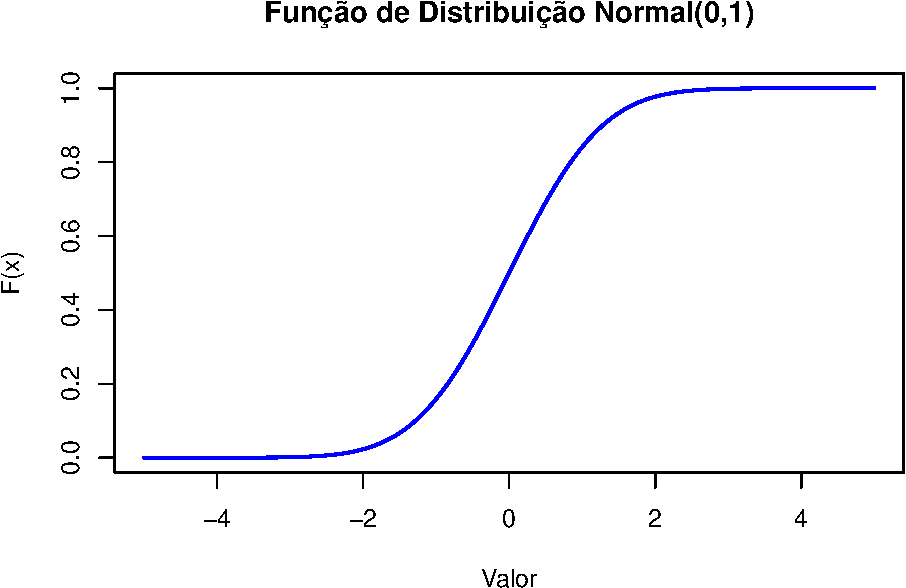
\includegraphics{introR_files/figure-latex/unnamed-chunk-200-1.pdf}

\textbf{Exemplo 1}: Resolva o exemplo 1 usando a função de distribuição empírica.

\begin{Shaded}
\begin{Highlighting}[]
\NormalTok{valores }\OtherTok{\textless{}{-}} \FunctionTok{rexp}\NormalTok{(}\DecValTok{10000}\NormalTok{, }\DecValTok{1}\SpecialCharTok{/}\DecValTok{30}\NormalTok{)}
\CommentTok{\# Função de distribuição empírica}
\NormalTok{Fn }\OtherTok{\textless{}{-}} \FunctionTok{ecdf}\NormalTok{(valores)}
\CommentTok{\# Probabilidade P(X\textless{}=20)}
\FunctionTok{Fn}\NormalTok{(}\DecValTok{20}\NormalTok{)}
\end{Highlighting}
\end{Shaded}

\begin{verbatim}
## [1] 0.4874
\end{verbatim}

\begin{Shaded}
\begin{Highlighting}[]
\CommentTok{\# Probabilidade exata}
\FunctionTok{pexp}\NormalTok{(}\DecValTok{20}\NormalTok{, }\DecValTok{1}\SpecialCharTok{/}\DecValTok{30}\NormalTok{)}
\end{Highlighting}
\end{Shaded}

\begin{verbatim}
## [1] 0.4865829
\end{verbatim}

\subsection{Função massa de probabilidade (teórica)}\label{funuxe7uxe3o-massa-de-probabilidade-teuxf3rica}

\begin{Shaded}
\begin{Highlighting}[]
\CommentTok{\# Simulação de Variáveis aleatórias}

\CommentTok{\# Função massa de probabilidade Binomial(n,p)}
\NormalTok{n }\OtherTok{\textless{}{-}} \DecValTok{20}
\NormalTok{p }\OtherTok{\textless{}{-}} \FloatTok{0.1}
\NormalTok{x }\OtherTok{\textless{}{-}} \DecValTok{0}\SpecialCharTok{:}\DecValTok{20}

\NormalTok{teorico }\OtherTok{\textless{}{-}} \FunctionTok{data.frame}\NormalTok{(}\AttributeTok{x =}\NormalTok{ x, }\AttributeTok{y=}\FunctionTok{dbinom}\NormalTok{(x, }\AttributeTok{size =}\NormalTok{ n, }\AttributeTok{prob =}\NormalTok{ p))}

\CommentTok{\# Carregue o pacote ggplot2}
\FunctionTok{library}\NormalTok{(ggplot2)}

\FunctionTok{ggplot}\NormalTok{(teorico) }\SpecialCharTok{+}  
  \FunctionTok{geom\_point}\NormalTok{(}\FunctionTok{aes}\NormalTok{(}\AttributeTok{x =}\NormalTok{ x, }\AttributeTok{y=}\NormalTok{y), }\AttributeTok{color =} \StringTok{"blue"}\NormalTok{) }\SpecialCharTok{+} 
  \FunctionTok{scale\_x\_continuous}\NormalTok{(}\AttributeTok{breaks =} \DecValTok{0}\SpecialCharTok{:}\NormalTok{n) }\SpecialCharTok{+}  
  \FunctionTok{labs}\NormalTok{(}\AttributeTok{title =} \StringTok{"Binomial(20,0.1)"}\NormalTok{, }\AttributeTok{x =} \StringTok{"Número de sucessos"}\NormalTok{, }\AttributeTok{y =} \StringTok{"Probabilidade"}\NormalTok{) }\SpecialCharTok{+}  
  \FunctionTok{theme\_light}\NormalTok{()}
\end{Highlighting}
\end{Shaded}

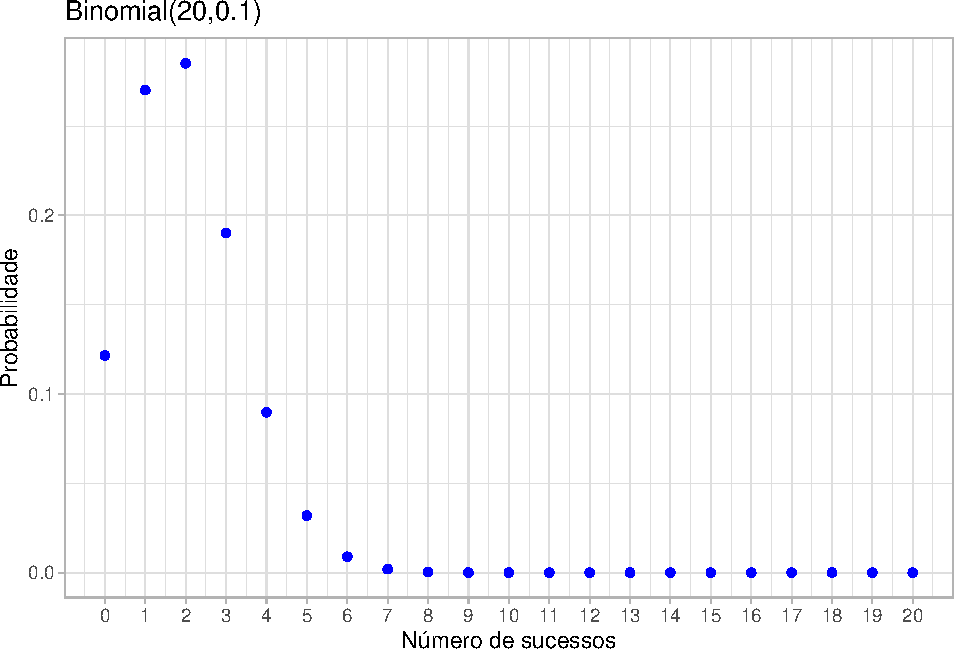
\includegraphics{introR_files/figure-latex/unnamed-chunk-202-1.pdf}

\subsection{Função massa de probabilidade (simulação)}\label{funuxe7uxe3o-massa-de-probabilidade-simulauxe7uxe3o}

\begin{Shaded}
\begin{Highlighting}[]
\FunctionTok{set.seed}\NormalTok{(}\DecValTok{1234}\NormalTok{)}

\NormalTok{n }\OtherTok{\textless{}{-}} \DecValTok{20}
\NormalTok{p }\OtherTok{\textless{}{-}} \FloatTok{0.9}
\NormalTok{k }\OtherTok{\textless{}{-}} \DecValTok{1000} \CommentTok{\# número de simulações}

\NormalTok{dados }\OtherTok{\textless{}{-}} \FunctionTok{data.frame}\NormalTok{(}\AttributeTok{X =} \FunctionTok{rbinom}\NormalTok{(k, }\AttributeTok{size =}\NormalTok{ n, }\AttributeTok{prob =}\NormalTok{ p))}

\CommentTok{\# Carregue o pacote ggplot2library(ggplot2)}

\FunctionTok{ggplot}\NormalTok{(dados) }\SpecialCharTok{+}   
\FunctionTok{geom\_bar}\NormalTok{(}\FunctionTok{aes}\NormalTok{(}\AttributeTok{x=}\NormalTok{X, }\AttributeTok{y=}\FunctionTok{after\_stat}\NormalTok{(prop)), }\AttributeTok{fill =} \StringTok{"lightblue"}\NormalTok{) }\SpecialCharTok{+}
  \FunctionTok{scale\_x\_continuous}\NormalTok{(}\AttributeTok{breaks =} \DecValTok{0}\SpecialCharTok{:}\NormalTok{n) }\SpecialCharTok{+}   
  \FunctionTok{labs}\NormalTok{(}\AttributeTok{title =} \StringTok{"Geração de números aleatórios de Bi(20,0.9)"}\NormalTok{, }\AttributeTok{x=}\StringTok{"Número de sucessos"}\NormalTok{, }
  \AttributeTok{y=}\StringTok{"Frequência relativa"}\NormalTok{) }\SpecialCharTok{+}  
  \FunctionTok{theme\_light}\NormalTok{()}
\end{Highlighting}
\end{Shaded}

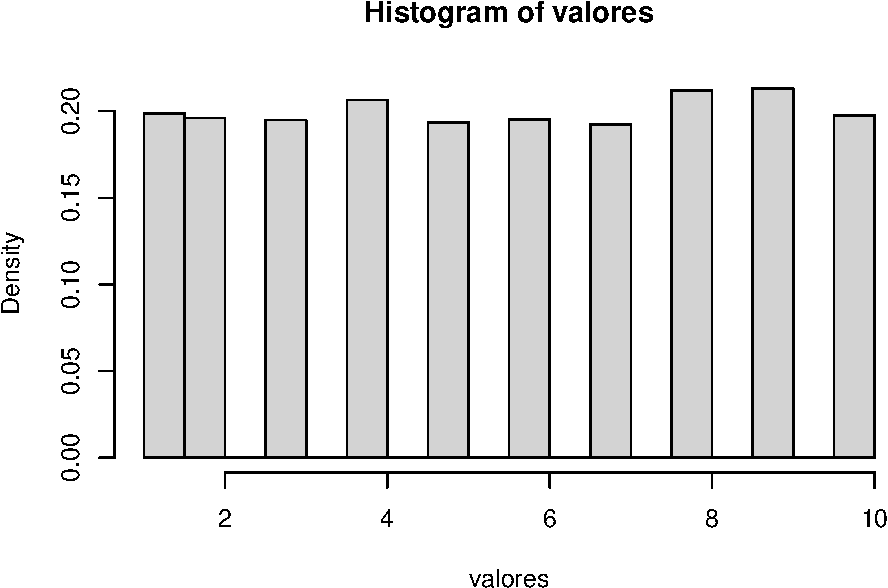
\includegraphics{introR_files/figure-latex/unnamed-chunk-203-1.pdf}

\subsection{Comparação}\label{comparauxe7uxe3o}

\begin{Shaded}
\begin{Highlighting}[]
\FunctionTok{set.seed}\NormalTok{(}\DecValTok{1234}\NormalTok{)}

\NormalTok{n }\OtherTok{\textless{}{-}} \DecValTok{20}
\NormalTok{p }\OtherTok{\textless{}{-}} \FloatTok{0.1}
\NormalTok{k }\OtherTok{\textless{}{-}} \DecValTok{1000} \CommentTok{\# número de simulações}

\NormalTok{dados }\OtherTok{\textless{}{-}} \FunctionTok{data.frame}\NormalTok{(}\AttributeTok{X =} \FunctionTok{rbinom}\NormalTok{(k, }\AttributeTok{size =}\NormalTok{ n, }\AttributeTok{prob =}\NormalTok{ p))}
\NormalTok{teorico }\OtherTok{\textless{}{-}} \FunctionTok{data.frame}\NormalTok{(}\AttributeTok{x =} \DecValTok{0}\SpecialCharTok{:}\NormalTok{n, }\AttributeTok{y=}\FunctionTok{dbinom}\NormalTok{(}\DecValTok{0}\SpecialCharTok{:}\NormalTok{n, }\AttributeTok{size =}\NormalTok{ n, }\AttributeTok{prob =}\NormalTok{ p))}

\CommentTok{\# Carregue o pacote ggplot2}
\FunctionTok{library}\NormalTok{(ggplot2)}

\FunctionTok{ggplot}\NormalTok{(dados) }\SpecialCharTok{+}  
  \FunctionTok{geom\_bar}\NormalTok{(}\FunctionTok{aes}\NormalTok{(}\AttributeTok{x =}\NormalTok{ X, }\AttributeTok{y =} \FunctionTok{after\_stat}\NormalTok{(prop)), }\AttributeTok{fill =} \StringTok{"lightblue"}\NormalTok{) }\SpecialCharTok{+} 
  \FunctionTok{geom\_point}\NormalTok{(}\AttributeTok{data =}\NormalTok{ teorico, }\FunctionTok{aes}\NormalTok{(x, y), }\AttributeTok{color =} \StringTok{"magenta"}\NormalTok{) }\SpecialCharTok{+} 
  \FunctionTok{scale\_x\_continuous}\NormalTok{(}\AttributeTok{breaks =} \DecValTok{0}\SpecialCharTok{:}\NormalTok{n) }\SpecialCharTok{+}  
  \FunctionTok{labs}\NormalTok{(}\AttributeTok{title =} \StringTok{"Geração de números aleatórios de Bi(20,0.1)"}\NormalTok{, }\AttributeTok{x =} \StringTok{"Número de sucessos"}\NormalTok{,       }
  \AttributeTok{y =} \StringTok{"Probabilidade"}\NormalTok{) }\SpecialCharTok{+}  
  \FunctionTok{theme\_light}\NormalTok{()}
\end{Highlighting}
\end{Shaded}

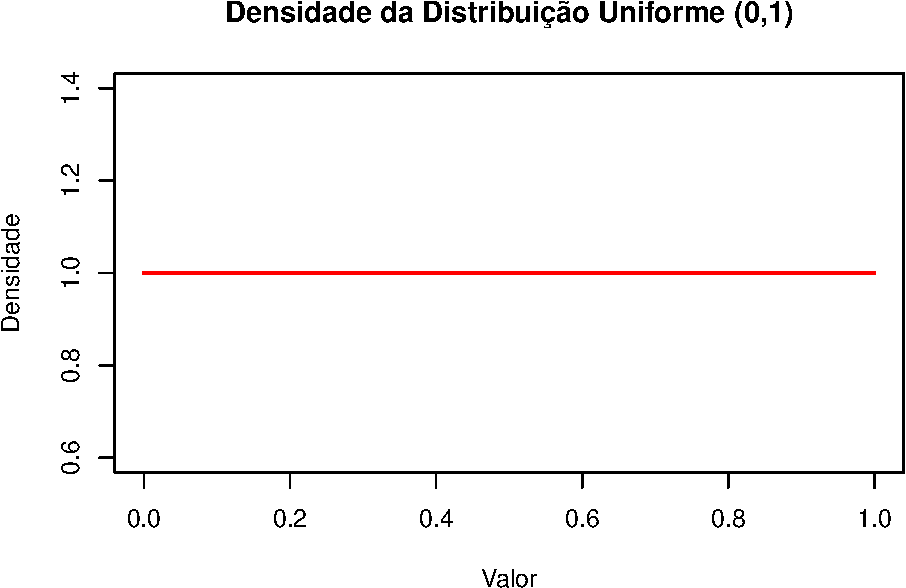
\includegraphics{introR_files/figure-latex/unnamed-chunk-204-1.pdf}

\subsection{Função de distribuição}\label{funuxe7uxe3o-de-distribuiuxe7uxe3o}

\begin{Shaded}
\begin{Highlighting}[]
\CommentTok{\# Definir os parâmetros da distribuição binomial}
\NormalTok{n }\OtherTok{\textless{}{-}} \DecValTok{10} \CommentTok{\# Número de tentativas}
\NormalTok{p }\OtherTok{\textless{}{-}} \FloatTok{0.5} \CommentTok{\# Probabilidade de sucesso}

\CommentTok{\# Valores possíveis de sucessos (0 a n)}
\NormalTok{x }\OtherTok{\textless{}{-}} \DecValTok{0}\SpecialCharTok{:}\NormalTok{n}

\CommentTok{\# Calcular a FD}
\NormalTok{cdf\_values }\OtherTok{\textless{}{-}} \FunctionTok{pbinom}\NormalTok{(x, }\AttributeTok{size =}\NormalTok{ n, }\AttributeTok{prob =}\NormalTok{ p)}

\CommentTok{\# Plotar a FD}
\FunctionTok{plot}\NormalTok{(x, cdf\_values, }\AttributeTok{type =} \StringTok{"s"}\NormalTok{, }\AttributeTok{lwd =} \DecValTok{2}\NormalTok{, }\AttributeTok{col =} \StringTok{"blue"}\NormalTok{, }
\AttributeTok{xlab =} \StringTok{"Número de Sucessos"}\NormalTok{, }\AttributeTok{ylab =} \StringTok{"F(x)"}\NormalTok{, }
\AttributeTok{main =} \StringTok{"Função de Distribuição Acumulada da Binomial(n = 10, p = 0.5)"}\NormalTok{)}
\end{Highlighting}
\end{Shaded}

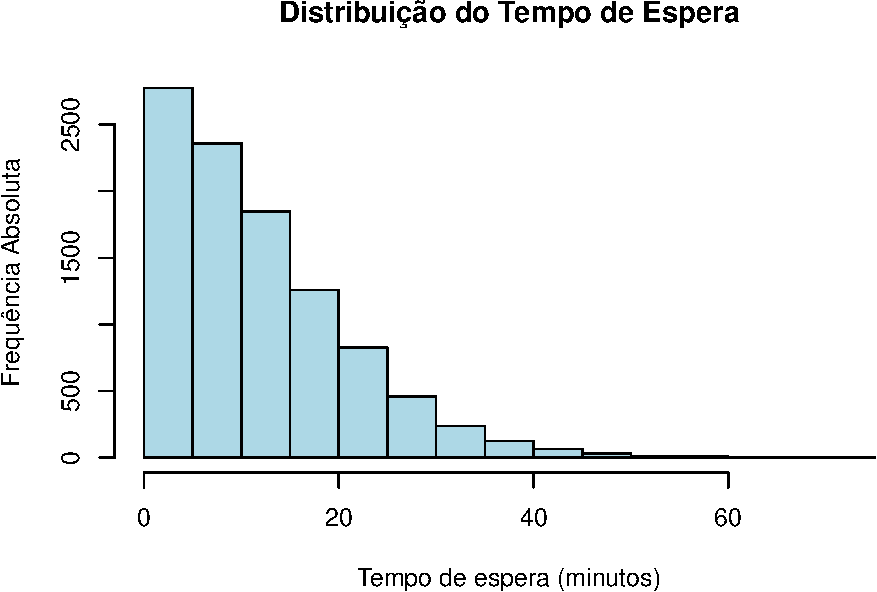
\includegraphics{introR_files/figure-latex/unnamed-chunk-205-1.pdf}

\subsection{Função de distribuição empírica}\label{funuxe7uxe3o-de-distribuiuxe7uxe3o-empuxedrica-1}

\begin{Shaded}
\begin{Highlighting}[]
\CommentTok{\# Definir os parâmetros da distribuição binomial}
\NormalTok{n }\OtherTok{\textless{}{-}} \DecValTok{10} \CommentTok{\# Número de tentativas}
\NormalTok{p }\OtherTok{\textless{}{-}} \FloatTok{0.5} \CommentTok{\# Probabilidade de sucesso}

\FunctionTok{set.seed}\NormalTok{(}\DecValTok{123}\NormalTok{)}
\CommentTok{\# Amostra aleatória de dimensão 1000}
\NormalTok{amostra }\OtherTok{\textless{}{-}} \FunctionTok{rbinom}\NormalTok{(}\DecValTok{1000}\NormalTok{,}\AttributeTok{size =}\NormalTok{ n, }\AttributeTok{prob =}\NormalTok{ p)}

\CommentTok{\# Distribuição empírica }
\NormalTok{Fn }\OtherTok{\textless{}{-}} \FunctionTok{ecdf}\NormalTok{(amostra)}

\CommentTok{\# Plotar CDF}
\FunctionTok{plot}\NormalTok{(Fn, }\AttributeTok{main =} \StringTok{"Função de Distribuição Empírica"}\NormalTok{, }\AttributeTok{xlab =} \StringTok{"x"}\NormalTok{, }
\AttributeTok{ylab =} \StringTok{"Fn(x)"}\NormalTok{, }\AttributeTok{col =} \StringTok{"blue"}\NormalTok{)}
\end{Highlighting}
\end{Shaded}

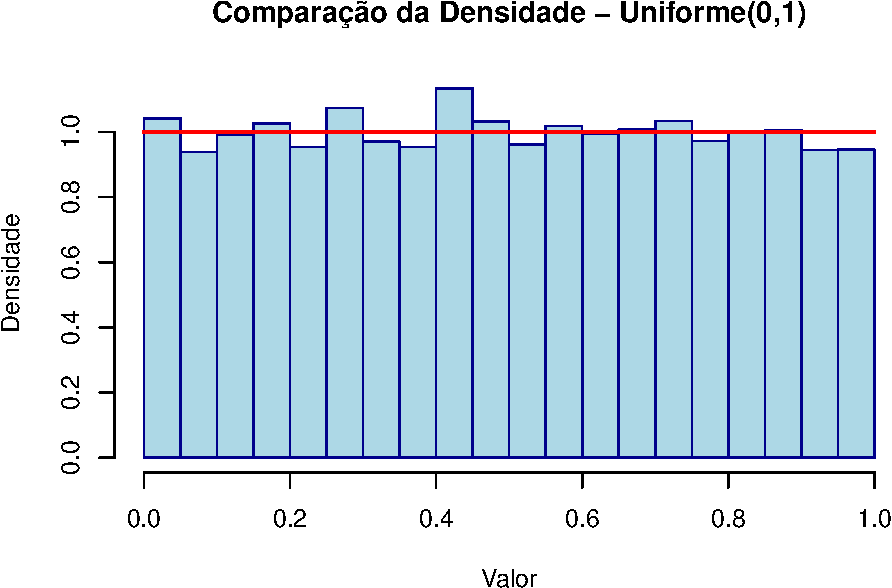
\includegraphics{introR_files/figure-latex/unnamed-chunk-206-1.pdf}

\begin{Shaded}
\begin{Highlighting}[]
\CommentTok{\# OU}
\FunctionTok{plot.ecdf}\NormalTok{(amostra)}
\end{Highlighting}
\end{Shaded}

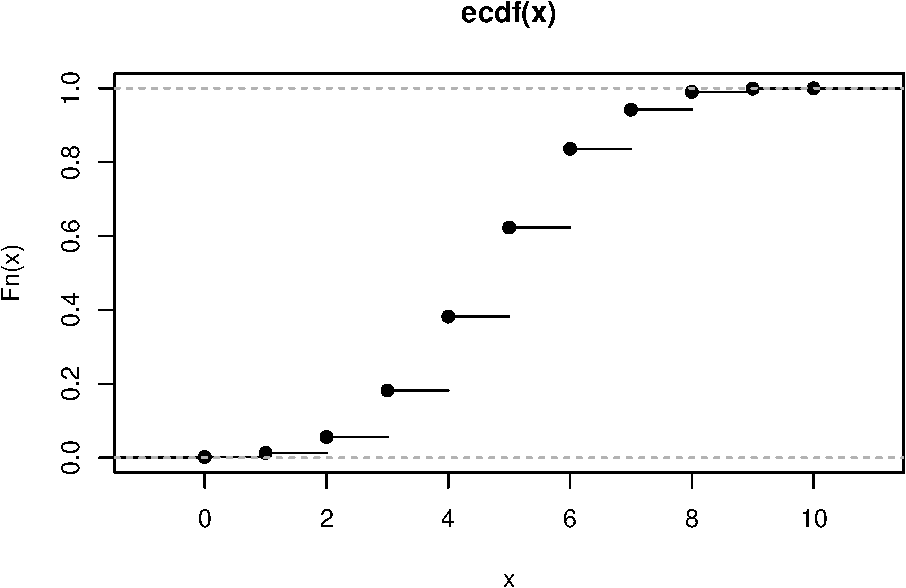
\includegraphics{introR_files/figure-latex/unnamed-chunk-206-2.pdf}

\textbf{Cálculo de probabilidade}: Seja
\(X \sim \text{Binomial}(n=10, p=0.5)\).

\(P(X \leq 4) =\) \texttt{pbinom(4,10,0.5)} = 0.377

\(P(X \leq 4) \approx\) \texttt{Fn(4)} = 0.382

\section{Gerando uma variável aleatória com distribuição de Poisson}\label{gerando-uma-variuxe1vel-aleatuxf3ria-com-distribuiuxe7uxe3o-de-poisson}

\subsection{Cálculo de probabilidades}\label{cuxe1lculo-de-probabilidades}

Seja \(X\sim\text{Poisson}(\lambda=5)\).

\(P(X =4) \to\) \texttt{dpois(4,5)} = 0.1755

\noindent \(P(X\leq 4) \to\) \texttt{ppois(4,5)} = 0.4405

\noindent \(P(X > 4)\to\) \texttt{ppois(4,5,lower.tail=FALSE)}= 0.5595

\subsection{Função massa de probabilidade (teórica)}\label{funuxe7uxe3o-massa-de-probabilidade-teuxf3rica-1}

\begin{Shaded}
\begin{Highlighting}[]
\CommentTok{\# Definir os valores de lambda e x}
\NormalTok{p }\OtherTok{\textless{}{-}} \FunctionTok{c}\NormalTok{(}\FloatTok{0.1}\NormalTok{, }\DecValTok{1}\NormalTok{, }\FloatTok{2.5}\NormalTok{, }\DecValTok{5}\NormalTok{, }\DecValTok{15}\NormalTok{, }\DecValTok{30}\NormalTok{)}
\NormalTok{x }\OtherTok{\textless{}{-}} \DecValTok{0}\SpecialCharTok{:}\DecValTok{50}

\CommentTok{\# Carregar os pacotes necessários}
\FunctionTok{library}\NormalTok{(ggplot2)}
\FunctionTok{library}\NormalTok{(latex2exp)}
\FunctionTok{library}\NormalTok{(gridExtra)}
\end{Highlighting}
\end{Shaded}

\begin{verbatim}
## 
## Attaching package: 'gridExtra'
\end{verbatim}

\begin{verbatim}
## The following object is masked from 'package:dplyr':
## 
##     combine
\end{verbatim}

\begin{Shaded}
\begin{Highlighting}[]
\CommentTok{\# Inicializar uma lista para armazenar os gráficos}
\NormalTok{plots }\OtherTok{\textless{}{-}} \FunctionTok{list}\NormalTok{()}

\CommentTok{\# Loop para criar os data frames e gráficos}
\ControlFlowTok{for}\NormalTok{ (i }\ControlFlowTok{in} \DecValTok{1}\SpecialCharTok{:}\FunctionTok{length}\NormalTok{(p)) \{  }
\NormalTok{  teorico }\OtherTok{\textless{}{-}} \FunctionTok{data.frame}\NormalTok{(}\AttributeTok{x =}\NormalTok{ x, }\AttributeTok{y =} \FunctionTok{dpois}\NormalTok{(x, }\AttributeTok{lambda =}\NormalTok{ p[i]))    }
    
\NormalTok{  plots[[i]] }\OtherTok{\textless{}{-}} \FunctionTok{ggplot}\NormalTok{(teorico) }\SpecialCharTok{+}    
    \FunctionTok{geom\_point}\NormalTok{(}\FunctionTok{aes}\NormalTok{(}\AttributeTok{x =}\NormalTok{ x, }\AttributeTok{y =}\NormalTok{ y), }\AttributeTok{color =} \StringTok{"blue"}\NormalTok{) }\SpecialCharTok{+} 
    \FunctionTok{scale\_x\_continuous}\NormalTok{(}\AttributeTok{breaks =} \FunctionTok{seq}\NormalTok{(}\DecValTok{0}\NormalTok{, }\DecValTok{50}\NormalTok{, }\AttributeTok{by =} \DecValTok{10}\NormalTok{)) }\SpecialCharTok{+}
    \FunctionTok{labs}\NormalTok{(}\AttributeTok{title =} \FunctionTok{TeX}\NormalTok{(}\FunctionTok{paste0}\NormalTok{(}\StringTok{"$Poisson(lambda="}\NormalTok{, p[i], }\StringTok{")$"}\NormalTok{)), }\AttributeTok{x=}\StringTok{"x"}\NormalTok{, }\AttributeTok{y=}\StringTok{"Probabilidade"}\NormalTok{) }\SpecialCharTok{+}
    \FunctionTok{theme\_light}\NormalTok{()}
\NormalTok{\}}
    
\CommentTok{\# Dispor os gráficos em uma grade 2x3}
\FunctionTok{grid.arrange}\NormalTok{(}\AttributeTok{grobs =}\NormalTok{ plots, }\AttributeTok{nrow =} \DecValTok{2}\NormalTok{, }\AttributeTok{ncol =} \DecValTok{3}\NormalTok{)}
\end{Highlighting}
\end{Shaded}

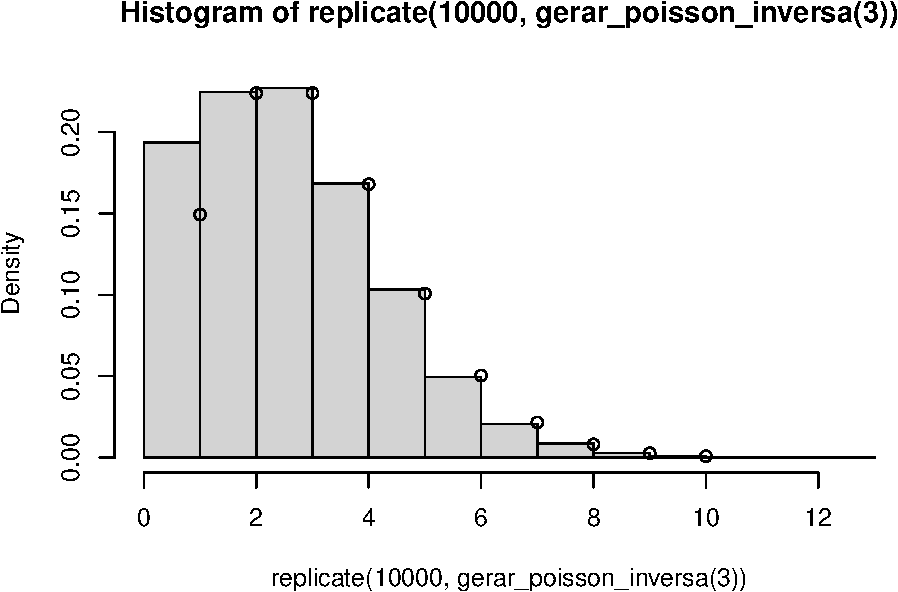
\includegraphics{introR_files/figure-latex/unnamed-chunk-207-1.pdf}

\subsection{Função massa de probabilidade (simulação)}\label{funuxe7uxe3o-massa-de-probabilidade-simulauxe7uxe3o-1}

\begin{Shaded}
\begin{Highlighting}[]
\NormalTok{p }\OtherTok{\textless{}{-}} \FunctionTok{c}\NormalTok{(}\FloatTok{0.1}\NormalTok{, }\DecValTok{1}\NormalTok{, }\FloatTok{2.5}\NormalTok{, }\DecValTok{5}\NormalTok{, }\DecValTok{15}\NormalTok{, }\DecValTok{30}\NormalTok{)}
\NormalTok{n }\OtherTok{\textless{}{-}} \DecValTok{1000}

\CommentTok{\# Carregar os pacotes necessários}
\FunctionTok{library}\NormalTok{(ggplot2)}
\FunctionTok{library}\NormalTok{(latex2exp)}
\FunctionTok{library}\NormalTok{(gridExtra)}

\CommentTok{\# Inicializar uma lista para armazenar os gráficos}
\NormalTok{plots }\OtherTok{\textless{}{-}} \FunctionTok{list}\NormalTok{()}

\CommentTok{\# Loop para criar os data frames e gráficos}
\ControlFlowTok{for}\NormalTok{ (i }\ControlFlowTok{in} \DecValTok{1}\SpecialCharTok{:}\FunctionTok{length}\NormalTok{(p)) \{  }
\NormalTok{  dados }\OtherTok{\textless{}{-}} \FunctionTok{data.frame}\NormalTok{(}\AttributeTok{X =} \FunctionTok{rpois}\NormalTok{(n, }\AttributeTok{lambda =}\NormalTok{ p[i]))}
  
\NormalTok{  plots[[i]] }\OtherTok{\textless{}{-}} \FunctionTok{ggplot}\NormalTok{(dados) }\SpecialCharTok{+}    
    \FunctionTok{geom\_bar}\NormalTok{(}\FunctionTok{aes}\NormalTok{(}\AttributeTok{x =}\NormalTok{ X, }\AttributeTok{y =}\FunctionTok{after\_stat}\NormalTok{(prop)), }\AttributeTok{fill=}\StringTok{"lightblue"}\NormalTok{) }\SpecialCharTok{+} 
    \FunctionTok{labs}\NormalTok{(}\AttributeTok{title=}\FunctionTok{TeX}\NormalTok{(}\FunctionTok{paste}\NormalTok{(}\StringTok{"$Poisson(lambda="}\NormalTok{, p[i], }\StringTok{")$"}\NormalTok{)), }
    \AttributeTok{x =} \StringTok{"x"}\NormalTok{, }\AttributeTok{y =} \StringTok{"Frequência relativa"}\NormalTok{) }\SpecialCharTok{+} 
    \FunctionTok{theme\_light}\NormalTok{()}
\NormalTok{\}}

\CommentTok{\# Dispor os gráficos em uma grade 2x3}
\FunctionTok{grid.arrange}\NormalTok{(}\AttributeTok{grobs =}\NormalTok{ plots, }\AttributeTok{nrow =} \DecValTok{2}\NormalTok{, }\AttributeTok{ncol =} \DecValTok{3}\NormalTok{)}
\end{Highlighting}
\end{Shaded}

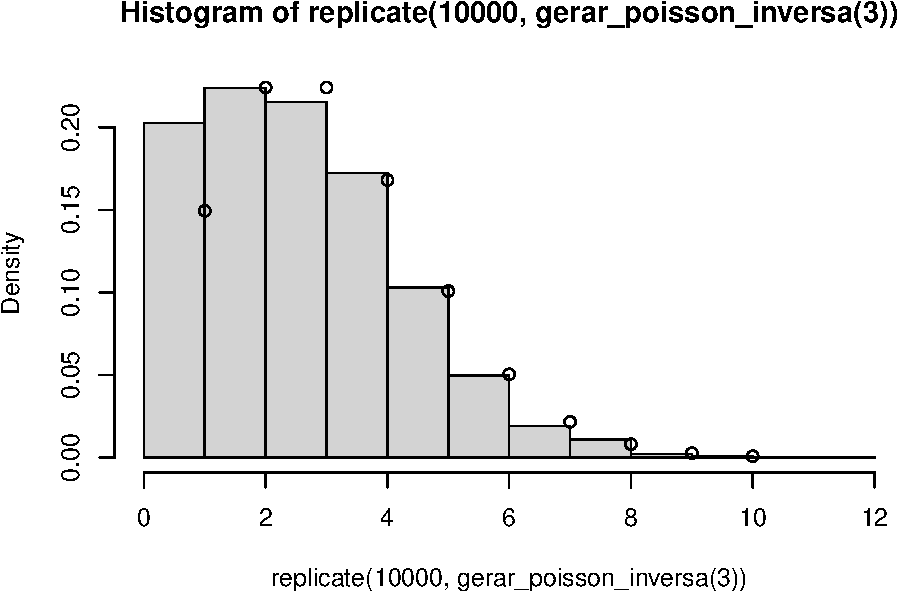
\includegraphics{introR_files/figure-latex/unnamed-chunk-208-1.pdf}

\subsection{Comparação}\label{comparauxe7uxe3o-1}

\begin{Shaded}
\begin{Highlighting}[]
\NormalTok{p }\OtherTok{\textless{}{-}} \FunctionTok{c}\NormalTok{(}\FloatTok{0.1}\NormalTok{, }\DecValTok{1}\NormalTok{, }\FloatTok{2.5}\NormalTok{, }\DecValTok{5}\NormalTok{, }\DecValTok{15}\NormalTok{, }\DecValTok{30}\NormalTok{)}
\NormalTok{n }\OtherTok{\textless{}{-}} \DecValTok{1000}

\CommentTok{\# Carregar os pacotes necessários}
\FunctionTok{library}\NormalTok{(ggplot2)}
\FunctionTok{library}\NormalTok{(latex2exp)}
\FunctionTok{library}\NormalTok{(gridExtra)}

\CommentTok{\# Inicializar uma lista para armazenar os gráficos}
\NormalTok{plots }\OtherTok{\textless{}{-}} \FunctionTok{list}\NormalTok{()}

\CommentTok{\# Loop para criar os data frames e gráficos}
\ControlFlowTok{for}\NormalTok{ (i }\ControlFlowTok{in} \DecValTok{1}\SpecialCharTok{:}\FunctionTok{length}\NormalTok{(p)) \{  }
\NormalTok{  dados }\OtherTok{\textless{}{-}} \FunctionTok{data.frame}\NormalTok{(}\AttributeTok{X =} \FunctionTok{rpois}\NormalTok{(n, }\AttributeTok{lambda =}\NormalTok{ p[i]))  }
\NormalTok{  teorico }\OtherTok{\textless{}{-}} \FunctionTok{data.frame}\NormalTok{(}\AttributeTok{x=}\DecValTok{0}\SpecialCharTok{:}\DecValTok{50}\NormalTok{, }\AttributeTok{y=}\FunctionTok{dpois}\NormalTok{(}\DecValTok{0}\SpecialCharTok{:}\DecValTok{50}\NormalTok{,p[i]))    }
  
\NormalTok{  plots[[i]] }\OtherTok{\textless{}{-}} \FunctionTok{ggplot}\NormalTok{(dados) }\SpecialCharTok{+}    
    \FunctionTok{geom\_bar}\NormalTok{(}\FunctionTok{aes}\NormalTok{(}\AttributeTok{x =}\NormalTok{ X, }\AttributeTok{y =}\FunctionTok{after\_stat}\NormalTok{(prop)), }\AttributeTok{fill=}\StringTok{"lightblue"}\NormalTok{) }\SpecialCharTok{+}    
    \FunctionTok{geom\_point}\NormalTok{(}\AttributeTok{data =}\NormalTok{ teorico, }\FunctionTok{aes}\NormalTok{(x, y), }\AttributeTok{color =} \StringTok{"magenta"}\NormalTok{) }\SpecialCharTok{+}    
    \FunctionTok{scale\_x\_continuous}\NormalTok{(}\AttributeTok{breaks =} \FunctionTok{seq}\NormalTok{(}\DecValTok{0}\NormalTok{, }\DecValTok{50}\NormalTok{, }\AttributeTok{by =} \DecValTok{10}\NormalTok{)) }\SpecialCharTok{+}
    \FunctionTok{labs}\NormalTok{(}\AttributeTok{title=}\FunctionTok{TeX}\NormalTok{(}\FunctionTok{paste}\NormalTok{(}\StringTok{"$Poisson(lambda="}\NormalTok{, p[i], }\StringTok{")$"}\NormalTok{)), }
    \AttributeTok{x =} \StringTok{"x"}\NormalTok{, }\AttributeTok{y =} \StringTok{"Frequência relativa"}\NormalTok{) }\SpecialCharTok{+}    
    \FunctionTok{theme\_light}\NormalTok{()}
\NormalTok{\}}

\CommentTok{\# Dispor os gráficos em uma grade 2x3}
\FunctionTok{grid.arrange}\NormalTok{(}\AttributeTok{grobs =}\NormalTok{ plots, }\AttributeTok{nrow =} \DecValTok{2}\NormalTok{, }\AttributeTok{ncol =} \DecValTok{3}\NormalTok{)}
\end{Highlighting}
\end{Shaded}

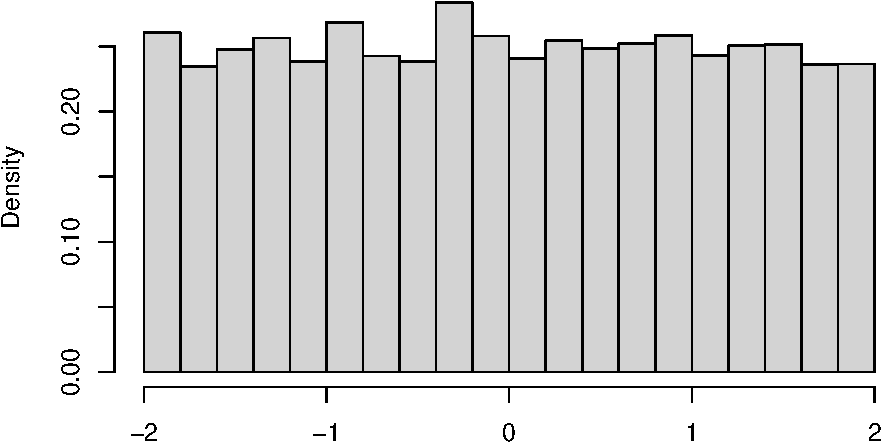
\includegraphics{introR_files/figure-latex/unnamed-chunk-209-1.pdf}

\subsection{Função de distribuição}\label{funuxe7uxe3o-de-distribuiuxe7uxe3o-1}

\begin{Shaded}
\begin{Highlighting}[]
\NormalTok{lambda }\OtherTok{\textless{}{-}} \DecValTok{5}  \CommentTok{\# Parâmetro da Poisson}
\NormalTok{x }\OtherTok{\textless{}{-}} \DecValTok{0}\SpecialCharTok{:}\DecValTok{15}    \CommentTok{\# Valores de x para plotar a distribuição}

\CommentTok{\# Calcular a FD}
\NormalTok{y }\OtherTok{\textless{}{-}} \FunctionTok{ppois}\NormalTok{(x, }\AttributeTok{lambda =}\NormalTok{ lambda)}

\CommentTok{\# Plotar a FD}
\FunctionTok{plot}\NormalTok{(x,y, }\AttributeTok{type=}\StringTok{"s"}\NormalTok{, }\AttributeTok{lwd=}\DecValTok{2}\NormalTok{, }\AttributeTok{col=}\StringTok{"blue"}\NormalTok{,     }
  \AttributeTok{main=}\FunctionTok{TeX}\NormalTok{(}\FunctionTok{paste}\NormalTok{(}\StringTok{"Função de Distribuição da $Poisson (lambda ="}\NormalTok{, lambda, }\StringTok{")$"}\NormalTok{)),    }
  \AttributeTok{xlab =} \StringTok{"x"}\NormalTok{,     }
  \AttributeTok{ylab =} \StringTok{"F(x)"}\NormalTok{)}
\end{Highlighting}
\end{Shaded}

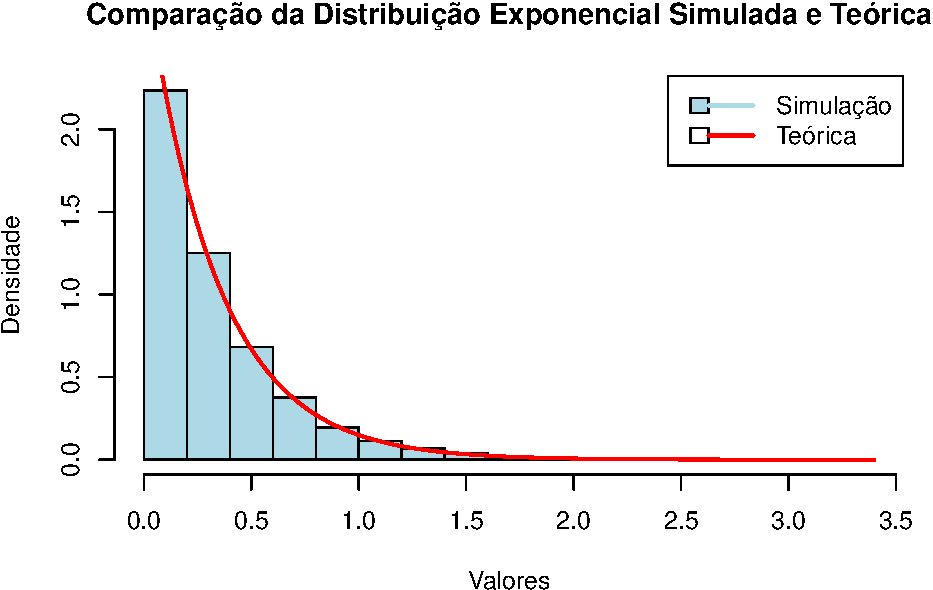
\includegraphics{introR_files/figure-latex/unnamed-chunk-210-1.pdf}

\subsection{Função de distribuição empírica}\label{funuxe7uxe3o-de-distribuiuxe7uxe3o-empuxedrica-2}

\begin{Shaded}
\begin{Highlighting}[]
\FunctionTok{library}\NormalTok{(latex2exp)}
\CommentTok{\# Definir os parâmetros da distribuição de Poisson}
\NormalTok{lambda }\OtherTok{\textless{}{-}} \DecValTok{5}

\NormalTok{dados }\OtherTok{\textless{}{-}} \FunctionTok{rpois}\NormalTok{(}\DecValTok{1000}\NormalTok{,}\AttributeTok{lambda =}\NormalTok{ lambda)}
\NormalTok{Fn }\OtherTok{\textless{}{-}} \FunctionTok{ecdf}\NormalTok{(dados)}

\CommentTok{\# Plotar CDF}
\FunctionTok{plot}\NormalTok{(Fn, }\AttributeTok{main=}\FunctionTok{TeX}\NormalTok{(}\StringTok{"Função de Distribuição Empírica da $Poisson(lambda = 5)$"}\NormalTok{),}
  \AttributeTok{xlab =} \StringTok{"x"}\NormalTok{,     }
  \AttributeTok{ylab =} \StringTok{"Fn(x)"}\NormalTok{,      }
  \AttributeTok{col =} \StringTok{"blue"}\NormalTok{)}
\end{Highlighting}
\end{Shaded}

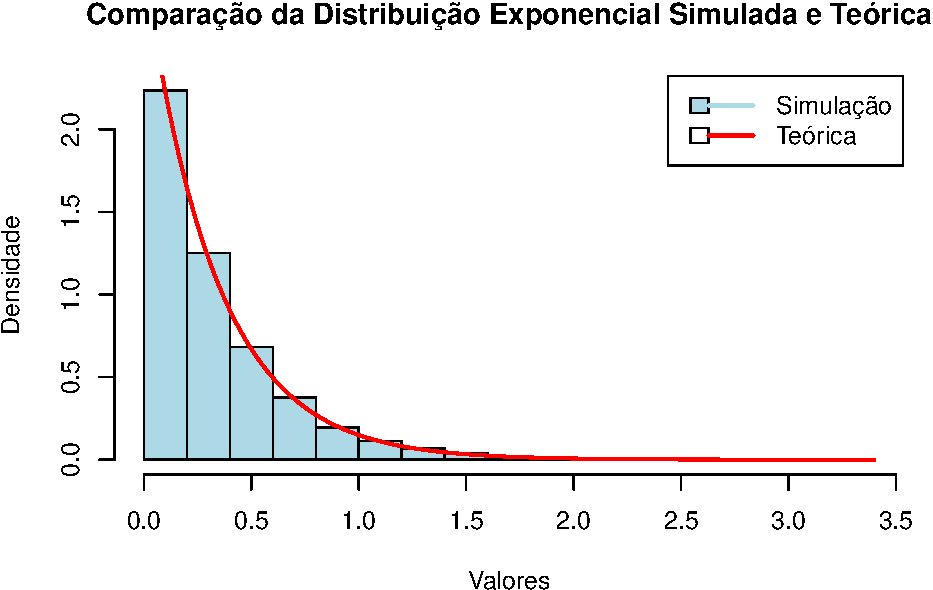
\includegraphics{introR_files/figure-latex/unnamed-chunk-211-1.pdf}

\begin{Shaded}
\begin{Highlighting}[]
\CommentTok{\# OU}
\CommentTok{\#plot.ecdf(dados)}

\FunctionTok{plot}\NormalTok{(Fn, }\AttributeTok{main=}\StringTok{"Função de Distribuição Empírica"}\NormalTok{,}
     \AttributeTok{xlab=}\StringTok{"x"}\NormalTok{,}
     \AttributeTok{ylab=}\StringTok{"Fn"}\NormalTok{,}
     \AttributeTok{col=}\StringTok{"blue"}\NormalTok{,}
     \AttributeTok{verticals =} \ConstantTok{TRUE}\NormalTok{)}
\end{Highlighting}
\end{Shaded}

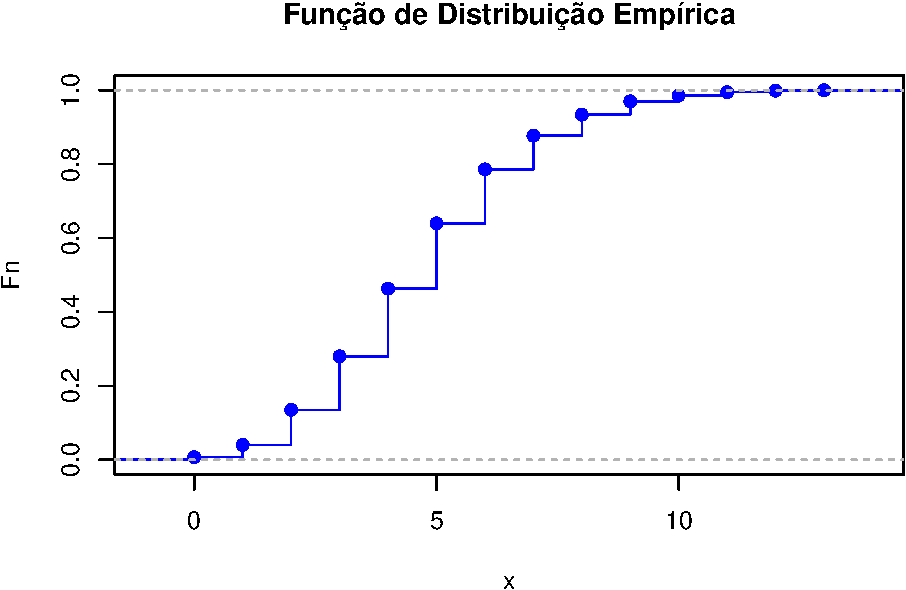
\includegraphics{introR_files/figure-latex/unnamed-chunk-211-2.pdf}

\textbf{Cálculo de probabilidades}: Seja \(X\sim\text{Poisson}(\lambda=5)\).

\(P(X\leq 4) \to\) \texttt{ppois(4,5)} = 0.4405

\(P(X \leq 4) \to\) \texttt{Fn(4)} = 0.433

\section{Gerando uma variável aleatória com distribuição de Uniforme}\label{gerando-uma-variuxe1vel-aleatuxf3ria-com-distribuiuxe7uxe3o-de-uniforme}

\subsection{Cálculo de probabilidades}\label{cuxe1lculo-de-probabilidades-1}

Seja \(X\sim \text{Uniforme}(0,1)\)

\begin{itemize}
\item
  \(P(X\leq 0.5) \to\) \texttt{punif(0.5,\ min\ =\ 0,\ max\ =\ 1)} = 0.5
\item
  \(P(X > 0.5) \to\) \texttt{punif(0.5,\ min\ =\ 0,\ max\ =\ 1,\ lower.tail\ =\ FALSE)}
  = 0.5
\end{itemize}

\subsection{Função densidade de probabilidade}\label{funuxe7uxe3o-densidade-de-probabilidade}

\begin{Shaded}
\begin{Highlighting}[]
\CommentTok{\# Gerar os valores x para a densidade teórica}
\NormalTok{x\_vals }\OtherTok{\textless{}{-}} \FunctionTok{seq}\NormalTok{(}\DecValTok{0}\NormalTok{, }\DecValTok{1}\NormalTok{, }\AttributeTok{length.out =} \DecValTok{100}\NormalTok{)}

\CommentTok{\# Calcular a densidade teórica para os valores x}
\NormalTok{y\_vals }\OtherTok{\textless{}{-}} \FunctionTok{dunif}\NormalTok{(x\_vals, }\AttributeTok{min =} \DecValTok{0}\NormalTok{, }\AttributeTok{max =} \DecValTok{1}\NormalTok{)}

\CommentTok{\# Desenhar o gráfico da função densidade de probabilidade}
\FunctionTok{plot}\NormalTok{(x\_vals, y\_vals, }\AttributeTok{type =} \StringTok{"l"}\NormalTok{, }
     \AttributeTok{col =} \StringTok{"red"}\NormalTok{, }\AttributeTok{lwd =} \DecValTok{2}\NormalTok{, }
     \AttributeTok{main =} \StringTok{"Densidade da Distribuição Uniforme (0,1)"}\NormalTok{,}
     \AttributeTok{xlab =} \StringTok{"Valor"}\NormalTok{, }\AttributeTok{ylab =} \StringTok{"Densidade"}\NormalTok{)}
\end{Highlighting}
\end{Shaded}

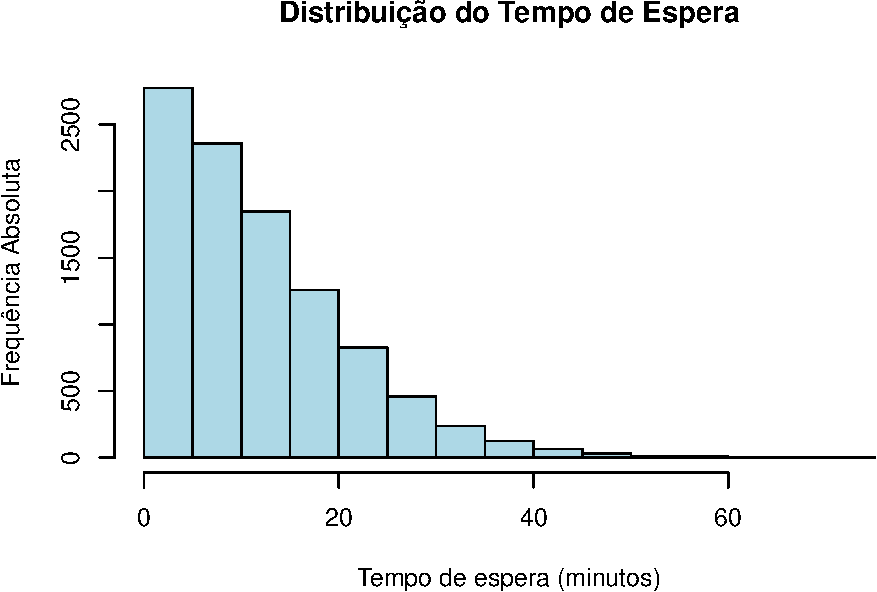
\includegraphics{introR_files/figure-latex/unnamed-chunk-212-1.pdf}

\subsection{Função densidade de probabilidade (simulação)}\label{funuxe7uxe3o-densidade-de-probabilidade-simulauxe7uxe3o}

\begin{Shaded}
\begin{Highlighting}[]
\CommentTok{\# Definir o tamanho da amostra}
\NormalTok{n }\OtherTok{\textless{}{-}} \DecValTok{10000}

\CommentTok{\# Fixar a semente para reprodutibilidade}
\FunctionTok{set.seed}\NormalTok{(}\DecValTok{123}\NormalTok{)}

\CommentTok{\# Gerar a variável aleatória com distribuição uniforme (0,1)}
\NormalTok{uniform\_data }\OtherTok{\textless{}{-}} \FunctionTok{runif}\NormalTok{(n, }\AttributeTok{min =} \DecValTok{0}\NormalTok{, }\AttributeTok{max =} \DecValTok{1}\NormalTok{)}

\CommentTok{\# Criar um histograma da amostra }
\FunctionTok{hist}\NormalTok{(uniform\_data, }\AttributeTok{probability =} \ConstantTok{TRUE}\NormalTok{, }
     \AttributeTok{main =} \StringTok{"Histograma da Densidade {-} Uniforme(0,1)"}\NormalTok{, }
     \AttributeTok{xlab =} \StringTok{"Valor"}\NormalTok{, }
     \AttributeTok{ylab =} \StringTok{"Densidade"}\NormalTok{, }
     \AttributeTok{col =} \StringTok{"lightblue"}\NormalTok{, }
     \AttributeTok{border =} \StringTok{"darkblue"}\NormalTok{)}
\end{Highlighting}
\end{Shaded}

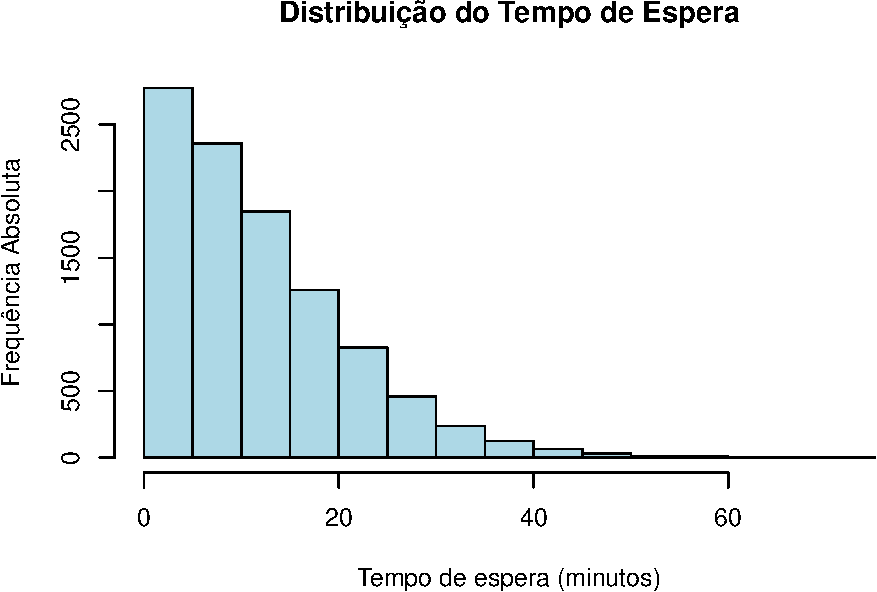
\includegraphics{introR_files/figure-latex/unnamed-chunk-213-1.pdf}

\subsection{Comparação}\label{comparauxe7uxe3o-2}

\begin{Shaded}
\begin{Highlighting}[]
\CommentTok{\# Definir o tamanho da amostra}
\NormalTok{n }\OtherTok{\textless{}{-}} \DecValTok{10000}

\CommentTok{\# Fixar a semente para reprodutibilidade}
\FunctionTok{set.seed}\NormalTok{(}\DecValTok{123}\NormalTok{)}

\CommentTok{\# Gerar a variável aleatória com distribuição uniforme (0,1)}
\NormalTok{uniform\_data }\OtherTok{\textless{}{-}} \FunctionTok{runif}\NormalTok{(n, }\AttributeTok{min =} \DecValTok{0}\NormalTok{, }\AttributeTok{max =} \DecValTok{1}\NormalTok{)}

\CommentTok{\# Criar um histograma da amostra com densidade}
\FunctionTok{hist}\NormalTok{(uniform\_data, }\AttributeTok{probability =} \ConstantTok{TRUE}\NormalTok{, }
     \AttributeTok{main =} \StringTok{"Comparação da Densidade {-} Uniforme(0,1)"}\NormalTok{, }
     \AttributeTok{xlab =} \StringTok{"Valor"}\NormalTok{, }
     \AttributeTok{ylab =} \StringTok{"Densidade"}\NormalTok{, }
     \AttributeTok{col =} \StringTok{"lightblue"}\NormalTok{, }
     \AttributeTok{border =} \StringTok{"darkblue"}\NormalTok{)}

\CommentTok{\# Adicionar a curva da densidade teórica}
\FunctionTok{curve}\NormalTok{(}\FunctionTok{dunif}\NormalTok{(x, }\AttributeTok{min =} \DecValTok{0}\NormalTok{, }\AttributeTok{max =} \DecValTok{1}\NormalTok{), }
      \AttributeTok{add =} \ConstantTok{TRUE}\NormalTok{, }
      \AttributeTok{col =} \StringTok{"red"}\NormalTok{, }
      \AttributeTok{lwd =} \DecValTok{2}\NormalTok{)}
\end{Highlighting}
\end{Shaded}

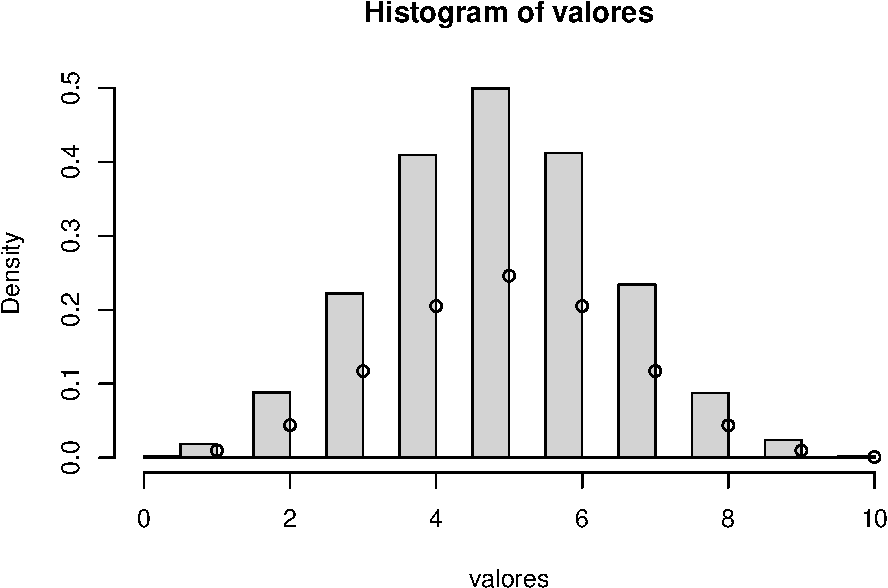
\includegraphics{introR_files/figure-latex/unnamed-chunk-214-1.pdf}

\subsection{Função de distribuição}\label{funuxe7uxe3o-de-distribuiuxe7uxe3o-2}

\begin{Shaded}
\begin{Highlighting}[]
\CommentTok{\# Gerar os valores x para a FD teórica}
\NormalTok{x\_vals }\OtherTok{\textless{}{-}} \FunctionTok{seq}\NormalTok{(}\DecValTok{0}\NormalTok{, }\DecValTok{1}\NormalTok{, }\AttributeTok{length.out =} \DecValTok{100}\NormalTok{)}

\CommentTok{\# Calcular a FD teórica para os valores x}
\NormalTok{y\_vals }\OtherTok{\textless{}{-}} \FunctionTok{punif}\NormalTok{(x\_vals, }\AttributeTok{min =} \DecValTok{0}\NormalTok{, }\AttributeTok{max =} \DecValTok{1}\NormalTok{)}

\CommentTok{\# Desenhar o gráfico da função de distribuição acumulada}
\FunctionTok{plot}\NormalTok{(x\_vals, y\_vals, }\AttributeTok{type =} \StringTok{"l"}\NormalTok{, }
     \AttributeTok{col =} \StringTok{"blue"}\NormalTok{, }\AttributeTok{lwd =} \DecValTok{2}\NormalTok{, }
     \AttributeTok{main =} \StringTok{"Função de Distribuição Uniforme (0,1)"}\NormalTok{,}
     \AttributeTok{xlab =} \StringTok{"Valor"}\NormalTok{, }\AttributeTok{ylab =} \StringTok{"F(x)"}\NormalTok{)}
\end{Highlighting}
\end{Shaded}

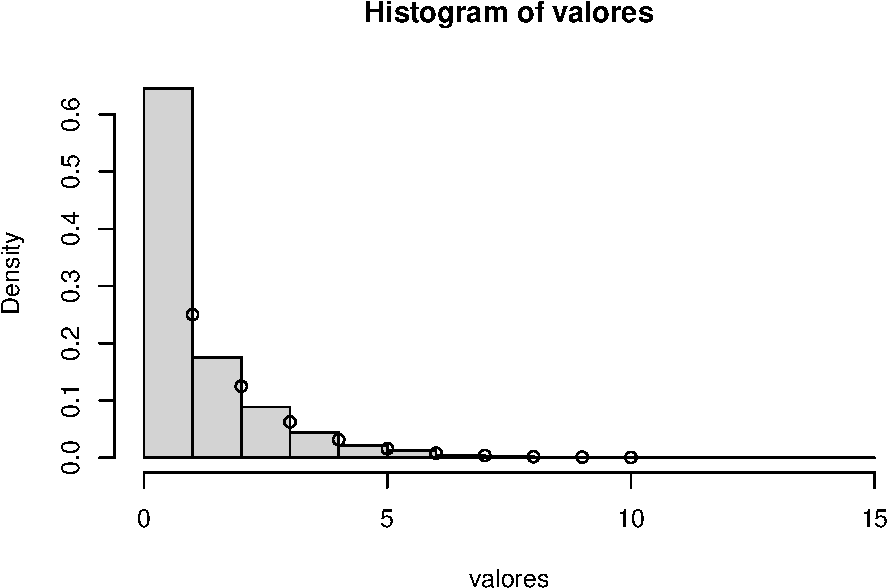
\includegraphics{introR_files/figure-latex/unnamed-chunk-215-1.pdf}

\subsection{Função de distribuição empírica}\label{funuxe7uxe3o-de-distribuiuxe7uxe3o-empuxedrica-3}

\begin{Shaded}
\begin{Highlighting}[]
\CommentTok{\# Definir o tamanho da amostra}
\NormalTok{n }\OtherTok{\textless{}{-}} \DecValTok{10000}

\CommentTok{\# Fixar a semente para reprodutibilidade}
\FunctionTok{set.seed}\NormalTok{(}\DecValTok{123}\NormalTok{)}

\CommentTok{\# Gerar a variável aleatória com distribuição uniforme (0,1)}
\NormalTok{uniform\_data }\OtherTok{\textless{}{-}} \FunctionTok{runif}\NormalTok{(n, }\AttributeTok{min =} \DecValTok{0}\NormalTok{, }\AttributeTok{max =} \DecValTok{1}\NormalTok{)}

\CommentTok{\# Função de distribuição empírica}
\NormalTok{Fn }\OtherTok{\textless{}{-}} \FunctionTok{ecdf}\NormalTok{(uniform\_data)}

\FunctionTok{plot}\NormalTok{(Fn, }\AttributeTok{main=}\StringTok{"Função de Distribuição Empírica"}\NormalTok{,}
     \AttributeTok{xlab=}\StringTok{"x"}\NormalTok{,}
     \AttributeTok{ylab=}\StringTok{"Fn"}\NormalTok{,}
     \AttributeTok{col=}\StringTok{"blue"}\NormalTok{)}
\end{Highlighting}
\end{Shaded}

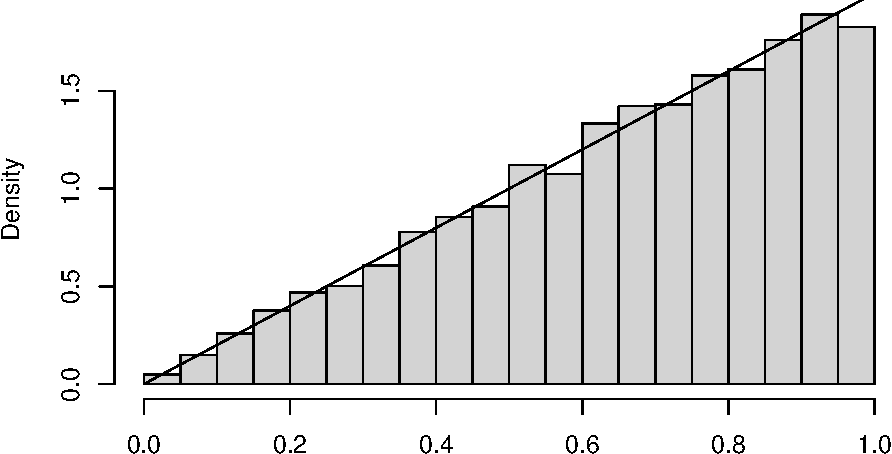
\includegraphics{introR_files/figure-latex/unnamed-chunk-216-1.pdf}

\begin{Shaded}
\begin{Highlighting}[]
\CommentTok{\# OU}
\CommentTok{\#plot.ecdf(uniform\_data)}
\end{Highlighting}
\end{Shaded}

\section{Gerando uma variável aleatória com distribuição Exponencial}\label{gerando-uma-variuxe1vel-aleatuxf3ria-com-distribuiuxe7uxe3o-exponencial}

\subsection{Cálculo de probabilidades}\label{cuxe1lculo-de-probabilidades-2}

Seja \(X\sim \text{Exponencial}(\lambda=1)\).

\(P(X\leq 0.5) \to\) \texttt{pexp(0.5,rate=1)}=0.3935

\(P(X > 0.5) \to\) \texttt{pexp(0.5,rate=1,lower.tail=FALSE)}=0.6065

\subsection{Função densidade de probabilidade (teórica)}\label{funuxe7uxe3o-densidade-de-probabilidade-teuxf3rica}

\begin{Shaded}
\begin{Highlighting}[]
\CommentTok{\# Gerar os valores x para a densidade teórica}
\NormalTok{x\_vals }\OtherTok{\textless{}{-}} \FunctionTok{seq}\NormalTok{(}\DecValTok{0}\NormalTok{, }\DecValTok{10}\NormalTok{, }\AttributeTok{length.out =} \DecValTok{100}\NormalTok{)}

\CommentTok{\# Calcular a densidade teórica para os valores x}
\NormalTok{y\_vals }\OtherTok{\textless{}{-}} \FunctionTok{dexp}\NormalTok{(x\_vals, }\AttributeTok{rate=}\DecValTok{1}\NormalTok{)}

\CommentTok{\# Desenhar o gráfico da função densidade de probabilidade}
\FunctionTok{plot}\NormalTok{(x\_vals, y\_vals, }\AttributeTok{type =} \StringTok{"l"}\NormalTok{, }
     \AttributeTok{col =} \StringTok{"red"}\NormalTok{, }\AttributeTok{lwd =} \DecValTok{2}\NormalTok{, }
     \AttributeTok{main =} \StringTok{"Densidade da Distribuição Exponencial(1)"}\NormalTok{,}
     \AttributeTok{xlab =} \StringTok{"Valor"}\NormalTok{, }\AttributeTok{ylab =} \StringTok{"Densidade"}\NormalTok{)}
\end{Highlighting}
\end{Shaded}

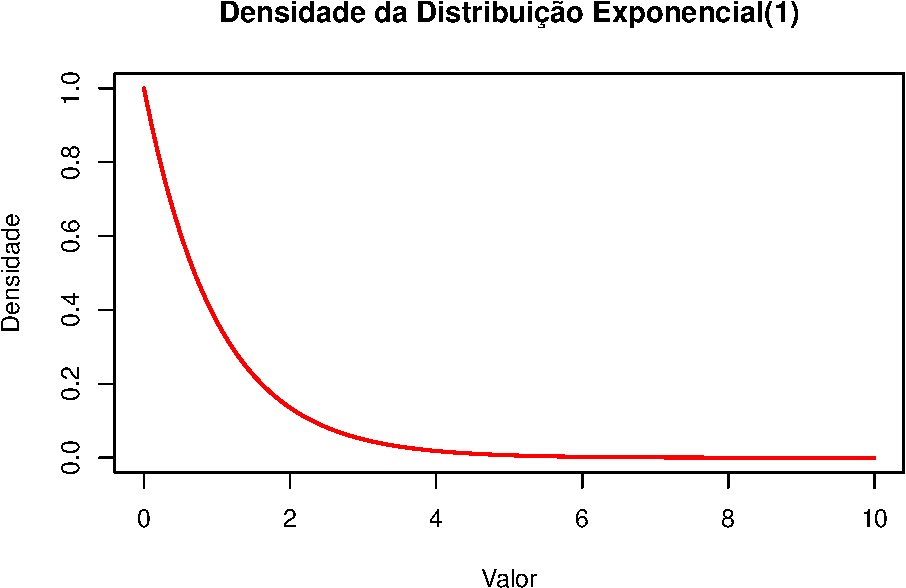
\includegraphics{introR_files/figure-latex/unnamed-chunk-217-1.pdf}

\subsection{Função densidade de probabilidade (simulação)}\label{funuxe7uxe3o-densidade-de-probabilidade-simulauxe7uxe3o-1}

\begin{Shaded}
\begin{Highlighting}[]
\CommentTok{\# Definir o tamanho da amostra}
\NormalTok{n }\OtherTok{\textless{}{-}} \DecValTok{10000}

\CommentTok{\# Fixar a semente para reprodutibilidade}
\FunctionTok{set.seed}\NormalTok{(}\DecValTok{123}\NormalTok{)}

\CommentTok{\# Gerar a variável aleatória com distribuição exponencial(1)}
\NormalTok{expo\_data }\OtherTok{\textless{}{-}} \FunctionTok{rexp}\NormalTok{(n, }\AttributeTok{rate=}\DecValTok{1}\NormalTok{)}

\CommentTok{\# Criar um histograma da amostra }
\FunctionTok{hist}\NormalTok{(expo\_data, }\AttributeTok{probability =} \ConstantTok{TRUE}\NormalTok{, }
     \AttributeTok{main =} \StringTok{"Histograma da Densidade {-} Exponencial(1)"}\NormalTok{, }
     \AttributeTok{xlab =} \StringTok{"Valor"}\NormalTok{, }
     \AttributeTok{ylab =} \StringTok{"Densidade"}\NormalTok{, }
     \AttributeTok{col =} \StringTok{"lightblue"}\NormalTok{, }
     \AttributeTok{border =} \StringTok{"darkblue"}\NormalTok{)}
\end{Highlighting}
\end{Shaded}

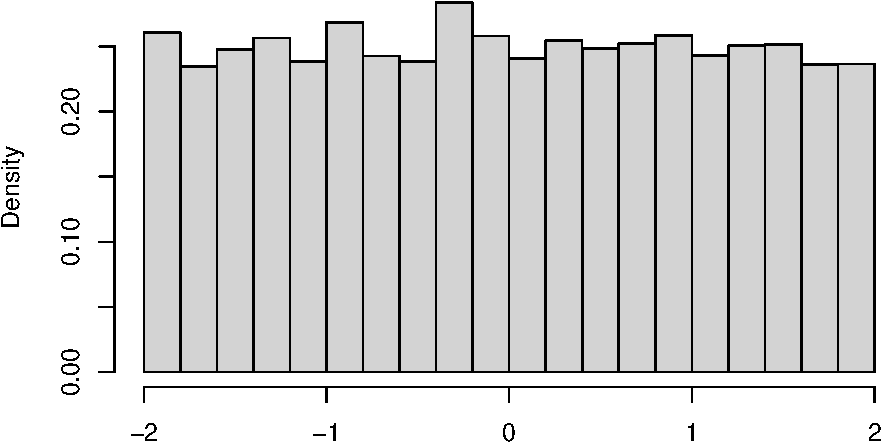
\includegraphics{introR_files/figure-latex/unnamed-chunk-218-1.pdf}

\subsection{Comparação}\label{comparauxe7uxe3o-3}

\begin{Shaded}
\begin{Highlighting}[]
\CommentTok{\# Definir o tamanho da amostra}
\NormalTok{n }\OtherTok{\textless{}{-}} \DecValTok{10000}

\CommentTok{\# Fixar a semente para reprodutibilidade}
\FunctionTok{set.seed}\NormalTok{(}\DecValTok{123}\NormalTok{)}

\CommentTok{\# Gerar a variável aleatória com distribuição exponencial(1)}
\NormalTok{expo\_data }\OtherTok{\textless{}{-}} \FunctionTok{rexp}\NormalTok{(n, }\AttributeTok{rate=}\DecValTok{1}\NormalTok{)}

\CommentTok{\# Criar um histograma da amostra }
\FunctionTok{hist}\NormalTok{(expo\_data, }\AttributeTok{probability =} \ConstantTok{TRUE}\NormalTok{, }
     \AttributeTok{main =} \StringTok{"Comparação da Densidade {-} Exponencial(1)"}\NormalTok{, }
     \AttributeTok{xlab =} \StringTok{"Valor"}\NormalTok{, }
     \AttributeTok{ylab =} \StringTok{"Densidade"}\NormalTok{, }
     \AttributeTok{col =} \StringTok{"lightblue"}\NormalTok{, }
     \AttributeTok{border =} \StringTok{"darkblue"}\NormalTok{)}

\CommentTok{\# Adicionar curva da densidade teórica}
\FunctionTok{curve}\NormalTok{(}\FunctionTok{dexp}\NormalTok{(x,}\AttributeTok{rate=}\DecValTok{1}\NormalTok{),}
      \AttributeTok{add=}\ConstantTok{TRUE}\NormalTok{,}
      \AttributeTok{col=}\StringTok{"red"}\NormalTok{,}
      \AttributeTok{lwd=}\DecValTok{2}\NormalTok{)}
\end{Highlighting}
\end{Shaded}

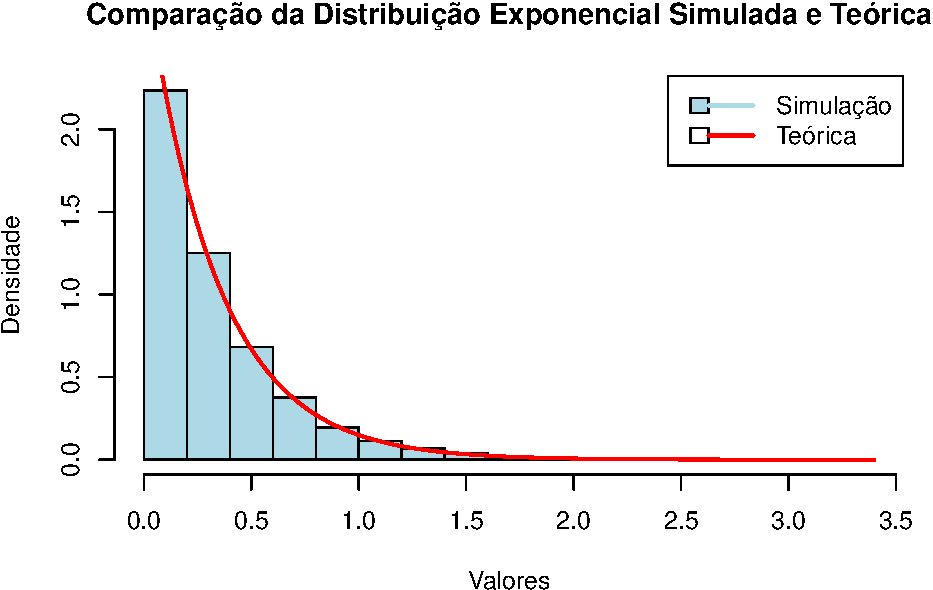
\includegraphics{introR_files/figure-latex/unnamed-chunk-219-1.pdf}

\subsection{Função de distribuição}\label{funuxe7uxe3o-de-distribuiuxe7uxe3o-3}

\begin{Shaded}
\begin{Highlighting}[]
\CommentTok{\# Gerar os valores x para a FD teórica}
\NormalTok{x\_vals }\OtherTok{\textless{}{-}} \FunctionTok{seq}\NormalTok{(}\DecValTok{0}\NormalTok{, }\DecValTok{10}\NormalTok{, }\AttributeTok{length.out =} \DecValTok{100}\NormalTok{)}

\CommentTok{\# Calcular a FD teórica para os valores x}
\NormalTok{y\_vals }\OtherTok{\textless{}{-}} \FunctionTok{pexp}\NormalTok{(x\_vals, }\AttributeTok{rate=}\DecValTok{1}\NormalTok{)}

\CommentTok{\# Desenhar o gráfico da FD}
\FunctionTok{plot}\NormalTok{(x\_vals, y\_vals, }\AttributeTok{type =} \StringTok{"l"}\NormalTok{, }
     \AttributeTok{col =} \StringTok{"red"}\NormalTok{, }\AttributeTok{lwd =} \DecValTok{2}\NormalTok{, }
     \AttributeTok{main =} \StringTok{"Função de Distribuição Exponencial(1)"}\NormalTok{,}
     \AttributeTok{xlab =} \StringTok{"Valor"}\NormalTok{, }\AttributeTok{ylab =} \StringTok{"F(x)"}\NormalTok{)}
\end{Highlighting}
\end{Shaded}

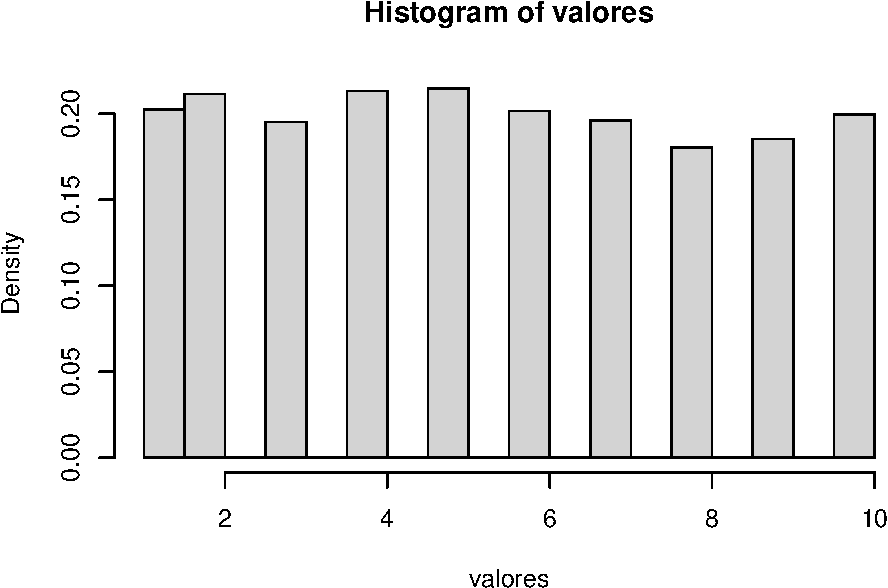
\includegraphics{introR_files/figure-latex/unnamed-chunk-220-1.pdf}

\subsection{Função de distribuição empírica}\label{funuxe7uxe3o-de-distribuiuxe7uxe3o-empuxedrica-4}

\begin{Shaded}
\begin{Highlighting}[]
\CommentTok{\# Definir o tamanho da amostra}
\NormalTok{n }\OtherTok{\textless{}{-}} \DecValTok{10000}

\CommentTok{\# Fixar a semente para reprodutibilidade}
\FunctionTok{set.seed}\NormalTok{(}\DecValTok{123}\NormalTok{)}

\CommentTok{\# Gerar a variável aleatória com distribuição exponencial(1)}
\NormalTok{expo\_data }\OtherTok{\textless{}{-}} \FunctionTok{rexp}\NormalTok{(n, }\AttributeTok{rate=}\DecValTok{1}\NormalTok{)}

\CommentTok{\# Função de distribuição empírica}
\NormalTok{Fn }\OtherTok{\textless{}{-}} \FunctionTok{ecdf}\NormalTok{(expo\_data)}

\FunctionTok{plot}\NormalTok{(Fn, }\AttributeTok{main=}\StringTok{"Função de Distribuição Empírica"}\NormalTok{,}
     \AttributeTok{xlab=}\StringTok{"x"}\NormalTok{,}
     \AttributeTok{ylab=}\StringTok{"Fn"}\NormalTok{,}
     \AttributeTok{col=}\StringTok{"blue"}\NormalTok{)}
\end{Highlighting}
\end{Shaded}

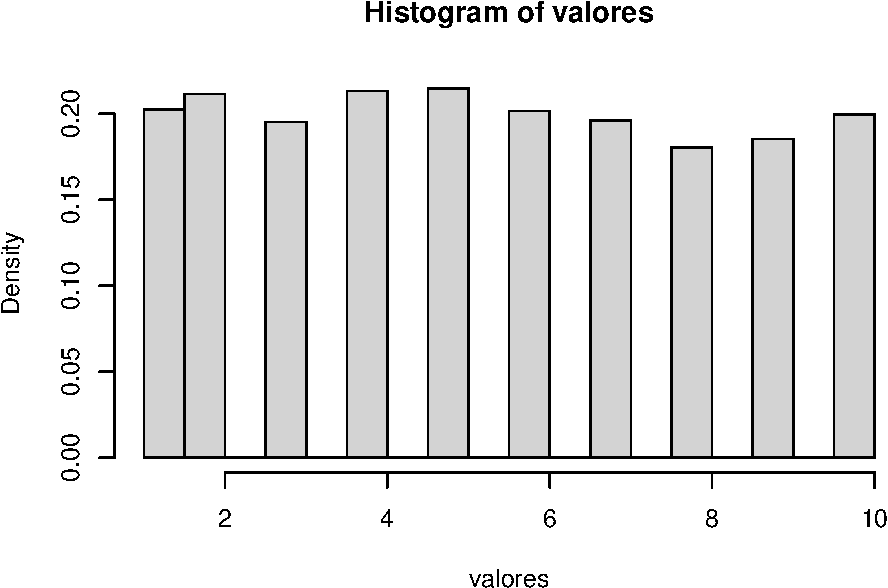
\includegraphics{introR_files/figure-latex/unnamed-chunk-221-1.pdf}

\section{Gerando uma variável aleatória com distribuição Normal}\label{gerando-uma-variuxe1vel-aleatuxf3ria-com-distribuiuxe7uxe3o-normal}

\subsection{Cálculo de probabilidades}\label{cuxe1lculo-de-probabilidades-3}

Seja \(X\sim \text{Normal}(0,1)\).

\(P(X \leq 0.5)\to\) \texttt{pnorm(0.5,mean=0,sd=1)}=0.6915

\(P(X >0.5)\to\) \texttt{pnorm(0.5,mean=0,sd=1,lower.tail=FALSE)}=0.3085

\subsection{Função densidade de probabilidade (teórica)}\label{funuxe7uxe3o-densidade-de-probabilidade-teuxf3rica-1}

\begin{Shaded}
\begin{Highlighting}[]
\CommentTok{\# Gerar os valores x para a densidade teórica}
\NormalTok{x\_vals }\OtherTok{\textless{}{-}} \FunctionTok{seq}\NormalTok{(}\SpecialCharTok{{-}}\DecValTok{5}\NormalTok{, }\DecValTok{5}\NormalTok{, }\AttributeTok{length.out =} \DecValTok{100}\NormalTok{)}

\CommentTok{\# Calcular a densidade teórica para os valores x}
\NormalTok{y\_vals }\OtherTok{\textless{}{-}} \FunctionTok{dnorm}\NormalTok{(x\_vals, }\AttributeTok{mean =} \DecValTok{0}\NormalTok{, }\AttributeTok{sd =} \DecValTok{1}\NormalTok{)}

\CommentTok{\# Desenhar o gráfico da função densidade de probabilidade}
\FunctionTok{plot}\NormalTok{(x\_vals, y\_vals, }\AttributeTok{type =} \StringTok{"l"}\NormalTok{, }
     \AttributeTok{col =} \StringTok{"red"}\NormalTok{, }\AttributeTok{lwd =} \DecValTok{2}\NormalTok{, }
     \AttributeTok{main =} \StringTok{"Densidade da Distribuição Normal(0,1)"}\NormalTok{,}
     \AttributeTok{xlab =} \StringTok{"Valor"}\NormalTok{, }\AttributeTok{ylab =} \StringTok{"Densidade"}\NormalTok{)}
\end{Highlighting}
\end{Shaded}

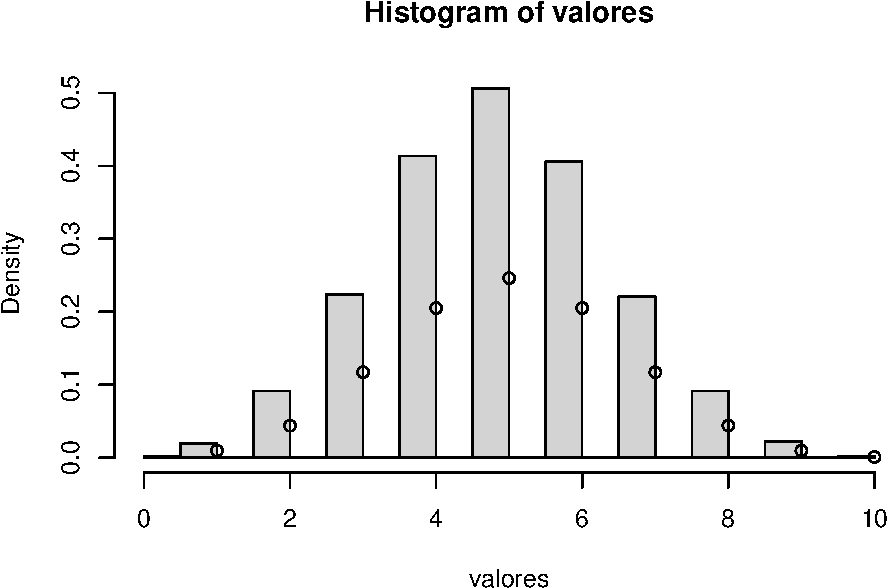
\includegraphics{introR_files/figure-latex/unnamed-chunk-222-1.pdf}

\subsection{Função densidade de probabilidade (simulação)}\label{funuxe7uxe3o-densidade-de-probabilidade-simulauxe7uxe3o-2}

\begin{Shaded}
\begin{Highlighting}[]
\CommentTok{\# Definir o tamanho da amostra}
\NormalTok{n }\OtherTok{\textless{}{-}} \DecValTok{10000}

\CommentTok{\# Fixar a semente para reprodutibilidade}
\FunctionTok{set.seed}\NormalTok{(}\DecValTok{123}\NormalTok{)}

\CommentTok{\# Gerar a variável aleatória com distribuição Normal(0,1)}
\NormalTok{normal\_data }\OtherTok{\textless{}{-}} \FunctionTok{rnorm}\NormalTok{(n, }\AttributeTok{mean =} \DecValTok{0}\NormalTok{, }\AttributeTok{sd =} \DecValTok{1}\NormalTok{)}

\CommentTok{\# Criar um histograma da amostra com densidade}
\FunctionTok{hist}\NormalTok{(normal\_data, }\AttributeTok{probability =} \ConstantTok{TRUE}\NormalTok{, }
     \AttributeTok{main =} \StringTok{"Comparação da Densidade {-} Normal(0,1)"}\NormalTok{, }
     \AttributeTok{xlab =} \StringTok{"Valor"}\NormalTok{, }
     \AttributeTok{ylab =} \StringTok{"Densidade"}\NormalTok{, }
     \AttributeTok{col =} \StringTok{"lightblue"}\NormalTok{, }
     \AttributeTok{border =} \StringTok{"darkblue"}\NormalTok{)}
\end{Highlighting}
\end{Shaded}

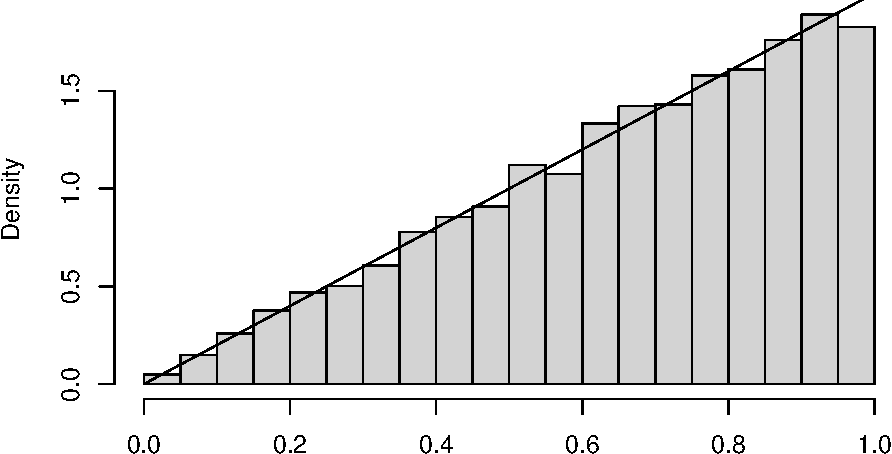
\includegraphics{introR_files/figure-latex/unnamed-chunk-223-1.pdf}

\subsection{Comparação}\label{comparauxe7uxe3o-4}

\begin{Shaded}
\begin{Highlighting}[]
\CommentTok{\# Definir o tamanho da amostra}
\NormalTok{n }\OtherTok{\textless{}{-}} \DecValTok{10000}

\CommentTok{\# Fixar a semente para reprodutibilidade}
\FunctionTok{set.seed}\NormalTok{(}\DecValTok{123}\NormalTok{)}

\CommentTok{\# Gerar a variável aleatória com distribuição Normal(0,1)}
\NormalTok{normal\_data }\OtherTok{\textless{}{-}} \FunctionTok{rnorm}\NormalTok{(n, }\AttributeTok{mean =} \DecValTok{0}\NormalTok{, }\AttributeTok{sd =} \DecValTok{1}\NormalTok{)}

\CommentTok{\# Criar um histograma da amostra com densidade}
\FunctionTok{hist}\NormalTok{(normal\_data, }\AttributeTok{probability =} \ConstantTok{TRUE}\NormalTok{, }
     \AttributeTok{main =} \StringTok{"Comparação da Densidade {-} Normal(0,1)"}\NormalTok{, }
     \AttributeTok{xlab =} \StringTok{"Valor"}\NormalTok{, }
     \AttributeTok{ylab =} \StringTok{"Densidade"}\NormalTok{, }
     \AttributeTok{col =} \StringTok{"lightblue"}\NormalTok{, }
     \AttributeTok{border =} \StringTok{"darkblue"}\NormalTok{)}

\CommentTok{\# Adicionar a curva da densidade teórica}
\FunctionTok{curve}\NormalTok{(}\FunctionTok{dnorm}\NormalTok{(x, }\AttributeTok{mean =} \DecValTok{0}\NormalTok{, }\AttributeTok{sd =} \DecValTok{1}\NormalTok{), }
      \AttributeTok{add =} \ConstantTok{TRUE}\NormalTok{, }
      \AttributeTok{col =} \StringTok{"red"}\NormalTok{, }
      \AttributeTok{lwd =} \DecValTok{2}\NormalTok{)}
\end{Highlighting}
\end{Shaded}

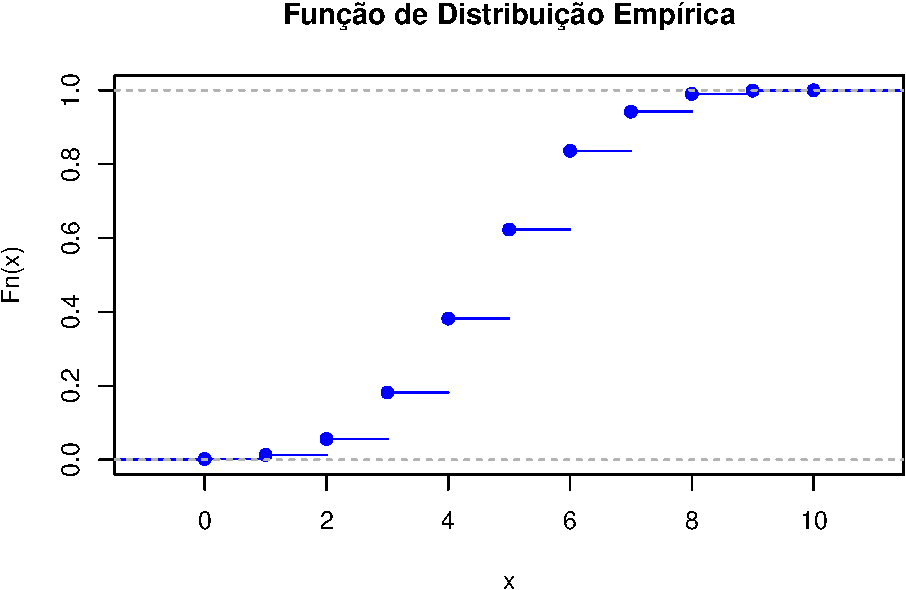
\includegraphics{introR_files/figure-latex/unnamed-chunk-224-1.pdf}

\subsection{Função de distribuição}\label{funuxe7uxe3o-de-distribuiuxe7uxe3o-4}

\begin{Shaded}
\begin{Highlighting}[]
\CommentTok{\# Gerar os valores x para a FD teórica}
\NormalTok{x\_vals }\OtherTok{\textless{}{-}} \FunctionTok{seq}\NormalTok{(}\SpecialCharTok{{-}}\DecValTok{5}\NormalTok{, }\DecValTok{5}\NormalTok{, }\AttributeTok{length.out =} \DecValTok{100}\NormalTok{)}

\CommentTok{\# Calcular a FD teórica para os valores x}
\NormalTok{y\_vals }\OtherTok{\textless{}{-}} \FunctionTok{pnorm}\NormalTok{(x\_vals, }\AttributeTok{mean =} \DecValTok{0}\NormalTok{, }\AttributeTok{sd =} \DecValTok{1}\NormalTok{)}

\CommentTok{\# Desenhar o gráfico da função de distribuição}
\FunctionTok{plot}\NormalTok{(x\_vals, y\_vals, }\AttributeTok{type =} \StringTok{"l"}\NormalTok{, }
     \AttributeTok{col =} \StringTok{"blue"}\NormalTok{, }\AttributeTok{lwd =} \DecValTok{2}\NormalTok{, }
     \AttributeTok{main =} \StringTok{"Função de Distribuição Normal(0,1)"}\NormalTok{,}
     \AttributeTok{xlab =} \StringTok{"Valor"}\NormalTok{, }\AttributeTok{ylab =} \StringTok{"F(x)"}\NormalTok{)}
\end{Highlighting}
\end{Shaded}

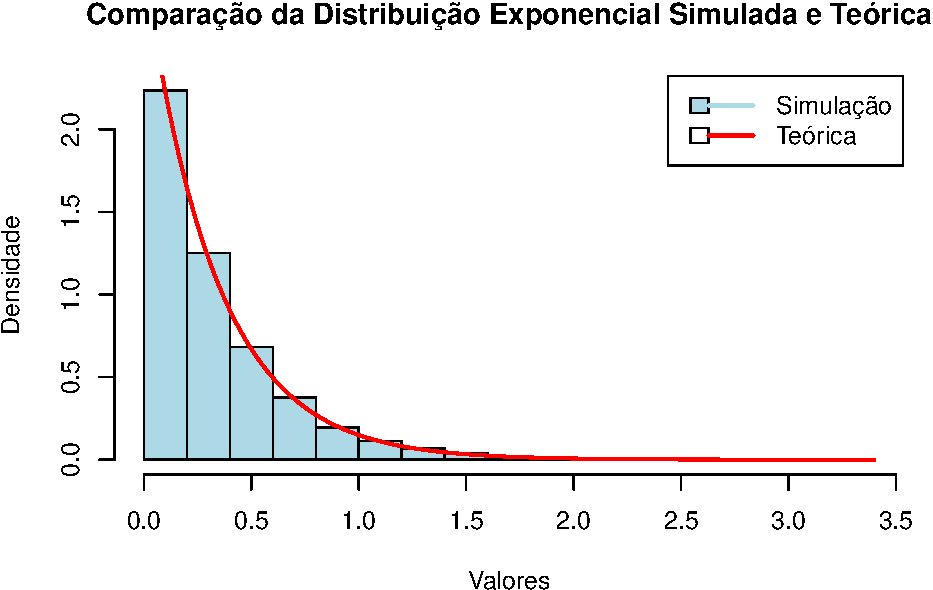
\includegraphics{introR_files/figure-latex/unnamed-chunk-225-1.pdf}

\subsection{Função de distribuição empírica}\label{funuxe7uxe3o-de-distribuiuxe7uxe3o-empuxedrica-5}

\begin{Shaded}
\begin{Highlighting}[]
\CommentTok{\# Definir o tamanho da amostra}
\NormalTok{n }\OtherTok{\textless{}{-}} \DecValTok{10000}

\CommentTok{\# Fixar a semente para reprodutibilidade}
\FunctionTok{set.seed}\NormalTok{(}\DecValTok{123}\NormalTok{)}

\CommentTok{\# Gerar a variável aleatória com distribuição Normal(0,1)}
\NormalTok{normal\_data }\OtherTok{\textless{}{-}} \FunctionTok{rnorm}\NormalTok{(n, }\AttributeTok{mean =} \DecValTok{0}\NormalTok{, }\AttributeTok{sd =} \DecValTok{1}\NormalTok{)}

\CommentTok{\# Função de distribuição empírica}
\NormalTok{Fn }\OtherTok{\textless{}{-}} \FunctionTok{ecdf}\NormalTok{(normal\_data)}

\FunctionTok{plot}\NormalTok{(Fn, }\AttributeTok{main=}\StringTok{"Função de Distribuição Empírica"}\NormalTok{,}
     \AttributeTok{xlab=}\StringTok{"x"}\NormalTok{,}
     \AttributeTok{ylab=}\StringTok{"Fn"}\NormalTok{,}
     \AttributeTok{col=}\StringTok{"blue"}\NormalTok{)}
\end{Highlighting}
\end{Shaded}

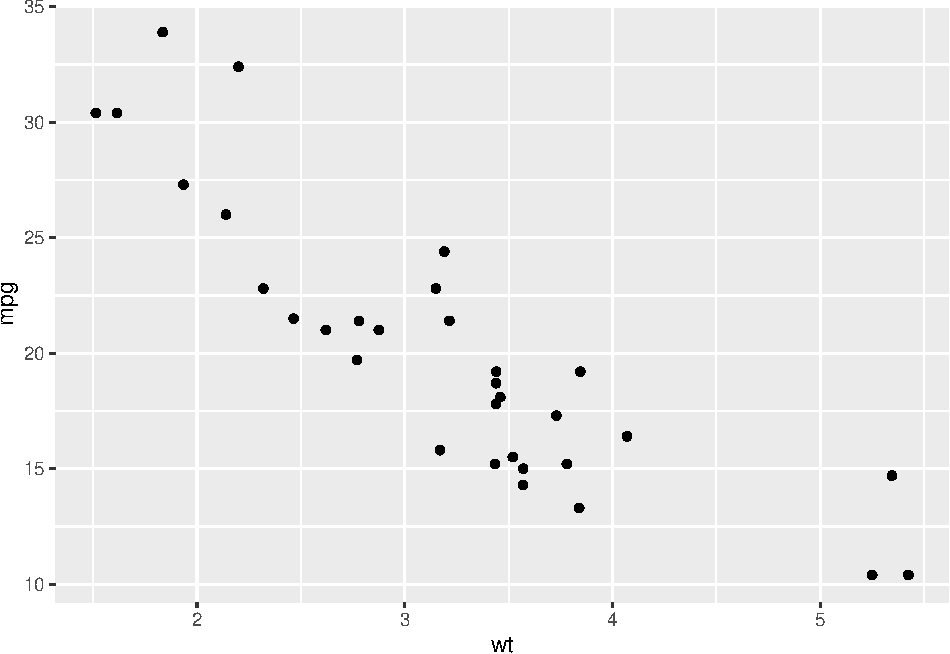
\includegraphics{introR_files/figure-latex/unnamed-chunk-226-1.pdf}

\section{Exercícios}\label{exercuxedcios-18}

\textbf{1.} Usando o R e fixando a semente em 123, simule 1000 lançamentos de
uma moeda com probabilidade de 0.5 de sair cara. Conte o número de caras
em cada lançamento e plote um histograma dos resultados.

\textbf{2.} Usando o R e fixando a semente em 123, gere uma amostra aleatória
de 5000 observações de uma variável aleatória binomial com parâmetros
\(n = 10\) e \(p = 0.3\). Calcule a média e a variância das observações
geradas.

\textbf{3.} Usando o R e fixando a semente em 123, gere uma amostra aleatória
de 2300 observações de uma variável aleatória de Poisson com parâmetro
\(\lambda = 4\). Calcule a média e o desvio padrão das observações
geradas.

\textbf{4.} Em um processo de qualidade, considere uma variável aleatória \(X\)
que representa o número de produtos defeituosos em um lote de 50
produtos, onde a probabilidade de um produto ser defeituoso é 0.1.
Usando o R e fixando a semente em 123 gere uma amostra aleatória de
10000 observações de \(X\). Conte a frequência de lotes com exatamente 5
produtos defeituosos. Calcule a proporção de lotes com exatamente 5
produtos defeituosos e compare o valor obtido com a probabilidade
\(P(X=5)\), onde \(X \sim \text{Binomial}(50, 0.1)\).

\textbf{5.} Usando o R e fixando a semente em 123, gere uma amostra aleatória
de 5000 observações de uma variável aleatória \(X\) binomial com
parâmetros \(n = 20\) e \(p = 0.7\).

\textbf{(a)} Faça um histograma de frequência relativa associado aos valores
amostrais. Sobreponha no gráfico a distribuição de probabilidade de \(X\).

\textbf{(b)} Use a função de distribuição empírica para estimar \(P(X\leq 10)\)
e compare com o valor teórico.

\textbf{6.} Usando o R e fixando a semente em 543, gere uma amostra aleatória
de 2400 observações de uma variável aleatória \(Y\) de Poisson com
parâmetro \(\lambda = 6\).

\textbf{(a)} Faça um histograma de frequência relativa associado aos valores
amostrais. Sobreponha no gráfico a distribuição de probabilidade de \(X\).

\textbf{(b)} Use a função de distribuição empírica para estimar \(P(Y > 5)\) e
compare com o valor teórico.

\textbf{7.} Usando o R e fixando a semente em 345, gere uma amostra aleatória
de 3450 observações de uma variável aleatória \(Z\) uniforme no intervalo
\([0, 1]\). Use a função de distribuição empírica para estimar
\(P(Z \leq 0.5)\) e compare com o valor teórico.

\textbf{8.} Usando o R e fixando a semente em 123, gere uma amostra aleatória
de 3467 observações de uma variável aleatória \(W\) normal com média
\(\mu = 0\) e desvio padrão \(\sigma = 1\).

\textbf{(a)} Faça um histograma de frequência relativa associado aos valores
amostrais. Sobreponha no gráfico a distribuição de \(X\).

\textbf{(b)} Use a função de distribuição empírica para estimar \(P(W > 1)\) e
compare com o valor teórico.

\textbf{9.} Usando o R e fixando a semente em 123, gere uma amostra aleatória
de 1234 observações de uma variável aleatória \(V\) exponencial com
parâmetro \(\lambda = 0.5\).

\textbf{(a)} Faça um histograma de frequência relativa associado aos valores
amostrais. Sobreponha no gráfico a distribuição de probabilidade de \(X\).

\textbf{(b)} Use a função de distribuição empírica para estimar \(P(V > 2)\) e
compare com o valor teórico.

\textbf{10.} O número de acertos num alvo em 30 tentativas onde a
probabilidade de acerto é 0.4, é modelado por uma variável aleatória \(X\)
com distruibuição Binomial de parâmetros \(n=30\) e \(p=0.4\). Usando o R e
fixando a semente em 123, gere uma amostra de dimensão \(n=700\) dessa
variável. Para essa amostra:

\textbf{(a)} Faça um histograma de frequência relativa associado aos valores
amostrais. Sobreponha no gráfico a distribuição de probabilidade de \(X\).

\textbf{(b)} Calcule a função de distribuição empírica e com base nessa
função estime a probabilidade do número de acertos no alvo, em 30
tentativas, ser maior que 15. Calcule ainda o valor teórico dessa
probabilidade.

\textbf{11.} Usando o R e fixando a semente em 123, gere amostras de tamanho
crescente \(n = 100, 1000, 10000, 100000\) de uma variável aleatória \(X\)
com distribuição de Poisson com parâmetro \(\lambda = 3\). Para cada
tamanho de amostra, calcule a média amostral e compare-a com o valor
esperado teórico. Observe e comente a convergência das médias amostrais.

\textbf{12.} Usando o R e fixando a semente em 123, gere amostras de tamanho
crescente \(n = 100, 1000, 10000, 100000\) de uma variável aleatória W com
distribuição uniforme no intervalo \([0, 1]\). Para cada tamanho de
amostra, calcule a média amostral e compare-a com o valor esperado
teórico. Observe e comente a convergência das médias amostrais.

\textbf{13.} Um grupo de estudantes de Estatística está realizando uma
pesquisa para avaliar o grau de satisfação dos alunos com um novo curso
oferecido pela universidade. Cada estudante responde a uma pergunta onde
pode indicar se está satisfeito ou insatisfeito com o curso. A
probabilidade de um estudante estar satisfeito é de \(0.75\).

\begin{itemize}
\tightlist
\item
  Usando o R e fixando a semente em 42, simule amostras de tamanho
  crescente \(n = 100, 500, 1000, 5000, 10000\) de uma variável
  aleatória \(X\) com distribuição binomial, onde \(X\) representa o
  número de estudantes satisfeitos. Para cada tamanho de amostra,
  calcule a proporção de estudantes satisfeitos e compare-a com a
  probabilidade teórica de satisfação (0.75).
\end{itemize}

\textbf{14.} Usando o R e fixando a semente em 1058, gere 9060 amostras de
dimensão 9 de uma população, \(X\sim \text{Binomial}(41,0.81)\). Calcule a
média de cada uma dessas amostras, obtendo uma amostra de médias.
Calcule ainda o valor esperado da distribuição teórica de \(X\) e compare
com a média da amostra de médias.

\textbf{15.} Em um hospital, o tempo de atendimento de pacientes segue uma
distribuição exponencial com média de 30 minutos. Um pesquisador deseja
estimar o tempo médio de atendimento coletando amostras de diferentes
tamanhos.

\begin{itemize}
\tightlist
\item
  Usando o R e fixando a semente em 456, simule 1000 amostras de
  tamanho 50, 100 e 1000 do tempo de atendimento. Para cada tamanho de
  amostra, calcule a média de cada amostra e plote o histograma das
  médias amostrais para cada tamanho. Compare essas distribuições com
  a distribuição normal com média \(E(X)\) e desvio padrão
  \(\sqrt{V(X)n}\) e comente sobre a aplicação do Teorema do Limite
  Central.
\end{itemize}

\textbf{16.} O tempo de espera (em minutos) para o atendimento no setor de
informações de um banco é modelado por uma variável aleatória X com
distribuição \text{Uniforme}(\(a=5, b=20\)). Usando o R e fixando a
semente em 1430, gere 8000 amostras de dimensão \(n=100\) dessa variável.
Para essas amostras:

\textbf{(a)} Calcule a soma de cada uma das amostras obtendo assim valores da
distribuição da soma \(S_{n} = \sum_{i=1}^{n}X_{n}\).

\textbf{(b)} Faça um histograma de frequência relativa associado aos valores
obtidos da distribuição da soma e sobreponha no gráfico uma curva com
distribuição normal de valor esperado \(nE(X)\) e desvio padrão
\(\sqrt{V(X)n}\).

\textbf{(c)} Calcule a média de cada uma das amostras obtendo assim valores
da distribuição da média \(\bar{X_{n}}\).

\textbf{(d)} Faça um histograma de frequência relativa associado aos valores
obtidos da distribuição da média \(\bar{X_{n}}\). Sobreponha no gráfico
uma curva com distribuição normal com valor esperado \(E(X)\) e desvio
padrão \(\sqrt{V(x)/n}\).

\textbf{17.} O tempo de atendimento (em minutos), de doentes graves num
determinado hospital, é modelado por uma variável aleatória \(X\) com
distribuição Exponencial(\(\lambda=0.21\)). Usando o R e fixando a semente
em 1580, gere 1234 amostras de dimensão \(n=50\) dessa variável. Para
essas amostras:

\textbf{(a)} Calcule a soma de cada uma das amostras obtendo assim valores da
distribuição da soma \(S_{n} = \sum_{i=1}^{n}X_{n}\).

\textbf{(b)} Faça um histograma de frequência relativa associado aos valores
obtidos da distribuição da soma e sobreponha no gráfico uma curva com
distribuição normal de valor esperado \(nE(X)\) e desvio padrão
\(\sqrt{V(X)n}\).

\textbf{(c)} Calcule agora a soma padronizada
\[\frac{S_{n}-E(S_{n})}{\sqrt{V(S_{n})}}\] e faça um histograma de
frequência relativa associado aos valores obtidos da distribuição da
soma padronizada. Sobreponha no gráfico uma curva com distribuição
normal de valor esperado 0 e desvio padrão 1.

\textbf{(d)} Calcule a média de cada uma das amostras obtendo assim valores
da distribuição da média \(\bar{X_{n}}\).

\textbf{(e)} Faça um histograma de frequência relativa associado aos valores
obtidos da distribuição da média \(\bar{X_{n}}\). Sobreponha no gráfico
uma curva com distribuição normal com valor esperado \(E(X)\) e desvio
padrão \(\sqrt{V(x)/n}\).

\textbf{18.} A altura (em centímetros) dos alunos de uma escola é modelada
por uma variável aleatória X com distribuição
\text{Normal}(\(\mu=170, \sigma=10\)). Usando o R e fixando a semente em
678, gere 9876 amostras de dimensão \(n=80\) dessa variável. Para essas
amostras:

\textbf{(a)} Calcule a soma de cada uma das amostras obtendo assim valores da
distribuição da soma \(S_{n} = \sum_{i=1}^{n}X_{n}\).

\textbf{(b)} Faça um histograma de frequência relativa associado aos valores
obtidos da distribuição da soma e sobreponha no gráfico uma curva com
distribuição normal de valor esperado \(nE(X)\) e desvio padrão
\(\sqrt{V(X)n}\).

\textbf{(c)} Calcule agora a soma padronizada
\[\frac{S_{n}-E(S_{n})}{\sqrt{V(S_{n})}}\] e faça um histograma de
frequência relativa associado aos valores obtidos da distribuição da
soma padronizada. Sobreponha no gráfico uma curva com distribuição
normal de valor esperado 0 e desvio padrão 1.

\textbf{(d)} Calcule a média de cada uma das amostras obtendo assim valores
da distribuição da média \(\bar{X_{n}}\).

\textbf{(e)} Faça um histograma de frequência relativa associado aos valores
obtidos da distribuição da média \(\bar{X_{n}}\). Sobreponha no gráfico
uma curva com distribuição normal com valor esperado \(E(X)\) e desvio
padrão \(\sqrt{V(x)/n}\).

\textbf{(f)} Faça um histograma de frequência relativa associado aos valores
obtidos da distribuição da média padronizada
\[\frac{\bar{X}_{n}-E(\bar{X_{n}})}{\sqrt{V(\bar{X_{n}})}}\] e
sobreponha no gráfico com uma curva com distribuição Normal com valor
esperado 0 e desvio padrão 1.

\textbf{19.} A chegada de clientes em uma loja durante 1 hora, assumindo uma
taxa média de 20 clientes por hora pode ser modelada por uma variável
aleatória \(X\) com distribuição de Poisson(\(\lambda=20\)). Usando o R e
fixando a semente em 1222, gere 8050 amostras de dimensão 30 de \(X\).

\textbf{(a)} Calcule a soma de cada uma das amostras obtendo assim valores da
distribuição da soma \(S_{n} = \sum_{i=1}^{n}X_{n}\).

\textbf{(b)} Faça um histograma de frequência relativa associado aos valores
obtidos da distribuição da soma e sobreponha no gráfico uma curva com
distribuição normal de valor esperado \(nE(X)\) e desvio padrão
\(\sqrt{V(X)n}\).

\textbf{(c)} Calcule agora a soma padronizada
\[\frac{S_{n}-E(S_{n})}{\sqrt{V(S_{n})}}\] e faça um histograma de
frequência relativa associado aos valores obtidos da distribuição da
soma padronizada. Sobreponha no gráfico uma curva com distribuição
normal de valor esperado 0 e desvio padrão 1.

\textbf{(d)} Calcule a média de cada uma das amostras obtendo assim valores
da distribuição da média \(\bar{X_{n}}\).

\textbf{(e)} Faça um histograma de frequência relativa associado aos valores
obtidos da distribuição da média \(\bar{X_{n}}\). Sobreponha no gráfico
uma curva com distribuição normal com valor esperado \(E(X)\) e desvio
padrão \(\sqrt{V(x)/n}\).

\textbf{(f)} Faça um histograma de frequência relativa associado aos valores
obtidos da distribuição da média padronizada
\[\frac{\bar{X}_{n}-E(\bar{X_{n}})}{\sqrt{V(\bar{X_{n}})}}\] e
sobreponha no gráfico com uma curva com distribuição Normal com valor
esperado 0 e desvio padrão 1.

\chapter{Relatórios}\label{relatuxf3rios}

\section{Markdown}\label{markdown}

\section{R Markdown}\label{r-markdown}

\chapter{Referências}\label{referuxeancias}

\begin{itemize}
\tightlist
\item
  \url{https://cemapre.iseg.ulisboa.pt/~nbrites/CTA/index.html}
\item
  \url{https://livro.curso-r.com/}
\end{itemize}

\chapter{Respostas}\label{respostas}

\section{O pacote dplyr}\label{o-pacote-dplyr-1}

\subsection{Selecionando colunas}\label{selecionando-colunas-1}

\textbf{1.} Teste aplicar a função \texttt{glimpse()} do pacote `\texttt{dplyr} à base
\texttt{sw}. O que ela faz?

\begin{Shaded}
\begin{Highlighting}[]
\FunctionTok{glimpse}\NormalTok{(sw)}
\end{Highlighting}
\end{Shaded}

\begin{verbatim}
## Rows: 87
## Columns: 14
## $ name       <chr> "Luke Skywalker", "C-3PO", "R2-D2", "Darth Vader", "Leia Or~
## $ height     <int> 172, 167, 96, 202, 150, 178, 165, 97, 183, 182, 188, 180, 2~
## $ mass       <dbl> 77.0, 75.0, 32.0, 136.0, 49.0, 120.0, 75.0, 32.0, 84.0, 77.~
## $ hair_color <chr> "blond", NA, NA, "none", "brown", "brown, grey", "brown", N~
## $ skin_color <chr> "fair", "gold", "white, blue", "white", "light", "light", "~
## $ eye_color  <chr> "blue", "yellow", "red", "yellow", "brown", "blue", "blue",~
## $ birth_year <dbl> 19.0, 112.0, 33.0, 41.9, 19.0, 52.0, 47.0, NA, 24.0, 57.0, ~
## $ sex        <chr> "male", "none", "none", "male", "female", "male", "female",~
## $ gender     <chr> "masculine", "masculine", "masculine", "masculine", "femini~
## $ homeworld  <chr> "Tatooine", "Tatooine", "Naboo", "Tatooine", "Alderaan", "T~
## $ species    <chr> "Human", "Droid", "Droid", "Human", "Human", "Human", "Huma~
## $ films      <list> <"A New Hope", "The Empire Strikes Back", "Return of the J~
## $ vehicles   <list> <"Snowspeeder", "Imperial Speeder Bike">, <>, <>, <>, "Imp~
## $ starships  <list> <"X-wing", "Imperial shuttle">, <>, <>, "TIE Advanced x1",~
\end{verbatim}

Mostra os nomes das variáveis, os tipos de dados e os primeiros valores
de cada coluna em uma única visualização, tudo de forma horizontal.

\textbf{2.} Crie uma tabela com apenas as colunas \texttt{name}, \texttt{gender}, e
\texttt{films}. Salve em um objeto chamado \texttt{sw\_simples}.

\begin{Shaded}
\begin{Highlighting}[]
\NormalTok{sw\_simples }\OtherTok{\textless{}{-}} \FunctionTok{select}\NormalTok{(sw, name, gender, films)}
\NormalTok{sw\_simples}
\end{Highlighting}
\end{Shaded}

\begin{verbatim}
## # A tibble: 87 x 3
##    name               gender    films    
##    <chr>              <chr>     <list>   
##  1 Luke Skywalker     masculine <chr [5]>
##  2 C-3PO              masculine <chr [6]>
##  3 R2-D2              masculine <chr [7]>
##  4 Darth Vader        masculine <chr [4]>
##  5 Leia Organa        feminine  <chr [5]>
##  6 Owen Lars          masculine <chr [3]>
##  7 Beru Whitesun Lars feminine  <chr [3]>
##  8 R5-D4              masculine <chr [1]>
##  9 Biggs Darklighter  masculine <chr [1]>
## 10 Obi-Wan Kenobi     masculine <chr [6]>
## # i 77 more rows
\end{verbatim}

\textbf{3.} Selecione apenas as colunas \texttt{hair\_color}, \texttt{skin\_color} e
\texttt{eye\_color} usando a função auxiliar \texttt{contains()}.

\begin{Shaded}
\begin{Highlighting}[]
\FunctionTok{select}\NormalTok{(sw, }\FunctionTok{contains}\NormalTok{(}\StringTok{"color"}\NormalTok{))}
\end{Highlighting}
\end{Shaded}

\begin{verbatim}
## # A tibble: 87 x 3
##    hair_color    skin_color  eye_color
##    <chr>         <chr>       <chr>    
##  1 blond         fair        blue     
##  2 <NA>          gold        yellow   
##  3 <NA>          white, blue red      
##  4 none          white       yellow   
##  5 brown         light       brown    
##  6 brown, grey   light       blue     
##  7 brown         light       blue     
##  8 <NA>          white, red  red      
##  9 black         light       brown    
## 10 auburn, white fair        blue-gray
## # i 77 more rows
\end{verbatim}

\textbf{4.} Usando a função \texttt{select()} (e suas funções auxiliares), escreva
códigos que retornem a base \texttt{sw} sem as colunas \texttt{hair\_color},
\texttt{skin\_color} e \texttt{eye\_color}. Escreva todas as soluções diferentes que
você conseguir pensar.

\begin{Shaded}
\begin{Highlighting}[]
\FunctionTok{select}\NormalTok{(sw, }\SpecialCharTok{{-}}\NormalTok{hair\_color, }\SpecialCharTok{{-}}\NormalTok{skin\_color, }\SpecialCharTok{{-}}\NormalTok{eye\_color)}

\FunctionTok{select}\NormalTok{(sw, }\SpecialCharTok{{-}}\FunctionTok{contains}\NormalTok{(}\StringTok{"color"}\NormalTok{))}

\FunctionTok{select}\NormalTok{(sw, }\SpecialCharTok{{-}}\FunctionTok{ends\_with}\NormalTok{(}\StringTok{"color"}\NormalTok{))}

\FunctionTok{select}\NormalTok{(sw, name}\SpecialCharTok{:}\NormalTok{mass, birth\_year}\SpecialCharTok{:}\NormalTok{starships)}
\end{Highlighting}
\end{Shaded}

\subsection{Ordenando a base}\label{ordenando-a-base-1}

\textbf{1.} Ordene \texttt{mass} em ordem crescente e \texttt{birth\_year} em ordem
decrescente e salve em um objeto chamado \texttt{sw\_ordenados}.

\begin{Shaded}
\begin{Highlighting}[]
\NormalTok{sw\_ordenados }\OtherTok{\textless{}{-}} \FunctionTok{arrange}\NormalTok{(sw, mass, }\FunctionTok{desc}\NormalTok{(birth\_year))}
\NormalTok{sw\_ordenados}
\end{Highlighting}
\end{Shaded}

\begin{verbatim}
## # A tibble: 87 x 14
##    name     height  mass hair_color skin_color eye_color birth_year sex   gender
##    <chr>     <int> <dbl> <chr>      <chr>      <chr>          <dbl> <chr> <chr> 
##  1 Ratts T~     79    15 none       grey, blue unknown           NA male  mascu~
##  2 Yoda         66    17 white      green      brown            896 male  mascu~
##  3 Wicket ~     88    20 brown      brown      brown              8 male  mascu~
##  4 R2-D2        96    32 <NA>       white, bl~ red               33 none  mascu~
##  5 R5-D4        97    32 <NA>       white, red red               NA none  mascu~
##  6 Sebulba     112    40 none       grey, red  orange            NA male  mascu~
##  7 Padmé A~    185    45 brown      light      brown             46 fema~ femin~
##  8 Dud Bolt     94    45 none       blue, grey yellow            NA male  mascu~
##  9 Wat Tam~    193    48 none       green, gr~ unknown           NA male  mascu~
## 10 Sly Moo~    178    48 none       pale       white             NA <NA>  <NA>  
## # i 77 more rows
## # i 5 more variables: homeworld <chr>, species <chr>, films <list>,
## #   vehicles <list>, starships <list>
\end{verbatim}

\textbf{2.} Selecione apenas as colunas \texttt{name} e \texttt{birth\_year} e então ordene
de forma decrescente pelo \texttt{birth\_year}.

\begin{Shaded}
\begin{Highlighting}[]
\CommentTok{\# Aninhando funções}
\FunctionTok{arrange}\NormalTok{(}\FunctionTok{select}\NormalTok{(sw, name, birth\_year), }\FunctionTok{desc}\NormalTok{(birth\_year))}

\CommentTok{\# Criando um objeto intermediário}
\NormalTok{sw\_aux }\OtherTok{\textless{}{-}} \FunctionTok{select}\NormalTok{(sw, name, birth\_year)}
\FunctionTok{arrange}\NormalTok{(sw\_aux, }\FunctionTok{desc}\NormalTok{(birth\_year))}

\CommentTok{\# Usando pipe}
\NormalTok{sw }\SpecialCharTok{\%\textgreater{}\%} 
  \FunctionTok{select}\NormalTok{(name, birth\_year) }\SpecialCharTok{\%\textgreater{}\%}
  \FunctionTok{arrange}\NormalTok{(}\FunctionTok{desc}\NormalTok{(birth\_year))}
\end{Highlighting}
\end{Shaded}

\subsection{Filtrando linhas}\label{filtrando-linhas-1}

Utilize a base \texttt{sw} nos exercícios a seguir.

\textbf{1.} Crie um objeto chamado \texttt{humanos} apenas com personagens que sejam
humanos.

\begin{Shaded}
\begin{Highlighting}[]
\NormalTok{humanos }\OtherTok{\textless{}{-}} \FunctionTok{filter}\NormalTok{(sw, species }\SpecialCharTok{==} \StringTok{"Human"}\NormalTok{)}

\CommentTok{\# O pipe}
\NormalTok{humanos }\OtherTok{\textless{}{-}}\NormalTok{ sw }\SpecialCharTok{\%\textgreater{}\%} 
  \FunctionTok{filter}\NormalTok{(species }\SpecialCharTok{==} \StringTok{"Human"}\NormalTok{)}
\end{Highlighting}
\end{Shaded}

\textbf{2.} Crie um objeto chamado \texttt{altos\_fortes} com personagens que tenham
mais de 200 cm de altura e peso maior que 100 kg.

\begin{Shaded}
\begin{Highlighting}[]
\NormalTok{altos\_fortes }\OtherTok{\textless{}{-}} \FunctionTok{filter}\NormalTok{(sw, height }\SpecialCharTok{\textgreater{}} \DecValTok{200}\NormalTok{, mass }\SpecialCharTok{\textgreater{}} \DecValTok{100}\NormalTok{)}
\end{Highlighting}
\end{Shaded}

\textbf{3.} Retorne tabelas (\texttt{tibbles}) apenas com:

\textbf{a.} Personagens humanos que nasceram antes de 100 anos antes da
batalha de Yavin (\texttt{birth\_year\ \textless{}\ 100}).

\begin{Shaded}
\begin{Highlighting}[]
\FunctionTok{filter}\NormalTok{(sw, species }\SpecialCharTok{==} \StringTok{"Human"}\NormalTok{, birth\_year }\SpecialCharTok{\textless{}} \DecValTok{100}\NormalTok{)}
\end{Highlighting}
\end{Shaded}

\textbf{b.} Personagens com cor \texttt{light} ou \texttt{red}.

\begin{Shaded}
\begin{Highlighting}[]
\FunctionTok{filter}\NormalTok{(sw, skin\_color }\SpecialCharTok{==} \StringTok{"light"} \SpecialCharTok{|}\NormalTok{ skin\_color }\SpecialCharTok{==} \StringTok{"red"}\NormalTok{)}
\end{Highlighting}
\end{Shaded}

\textbf{c.} Personagens com massa maior que 100 kg, ordenados de forma
decrescente por altura, mostrando apenas as colunas \texttt{name}, \texttt{mass} e
\texttt{height}.

\begin{Shaded}
\begin{Highlighting}[]
\FunctionTok{select}\NormalTok{(}\FunctionTok{arrange}\NormalTok{(}\FunctionTok{filter}\NormalTok{(sw, mass }\SpecialCharTok{\textgreater{}} \DecValTok{100}\NormalTok{), }\FunctionTok{desc}\NormalTok{(height)), name, mass, height)}

\CommentTok{\# usando o pipe}
\NormalTok{sw }\SpecialCharTok{\%\textgreater{}\%} 
  \FunctionTok{filter}\NormalTok{(mass }\SpecialCharTok{\textgreater{}} \DecValTok{100}\NormalTok{) }\SpecialCharTok{\%\textgreater{}\%} 
  \FunctionTok{arrange}\NormalTok{(}\FunctionTok{desc}\NormalTok{(height)) }\SpecialCharTok{\%\textgreater{}\%} 
  \FunctionTok{select}\NormalTok{(name, mass, height)}
\end{Highlighting}
\end{Shaded}

\textbf{d.} Personagens que sejam ``Humano'' ou ``Droid'', e tenham uma altura
maior que 170 cm.

\begin{Shaded}
\begin{Highlighting}[]
\FunctionTok{filter}\NormalTok{(sw, species }\SpecialCharTok{==} \StringTok{"Human"} \SpecialCharTok{|}\NormalTok{ species }\SpecialCharTok{==} \StringTok{"Droid"}\NormalTok{, height }\SpecialCharTok{\textgreater{}} \DecValTok{170}\NormalTok{)}

\CommentTok{\# usando o pipe}
\NormalTok{sw }\SpecialCharTok{\%\textgreater{}\%} 
  \FunctionTok{filter}\NormalTok{(species }\SpecialCharTok{\%in\%} \FunctionTok{c}\NormalTok{(}\StringTok{"Human"}\NormalTok{, }\StringTok{"Droid"}\NormalTok{), height }\SpecialCharTok{\textgreater{}} \DecValTok{170}\NormalTok{)}
\end{Highlighting}
\end{Shaded}

\textbf{e.} Personagens que não possuem informação tanto de altura quanto de
massa, ou seja, possuem NA em ambas as colunas.

\begin{Shaded}
\begin{Highlighting}[]
\FunctionTok{filter}\NormalTok{(sw, }\FunctionTok{is.na}\NormalTok{(height), }\FunctionTok{is.na}\NormalTok{(mass))}
\end{Highlighting}
\end{Shaded}

\subsection{Modificando e criando novas colunas}\label{modificando-e-criando-novas-colunas-1}

\textbf{1.} Crie uma coluna chamada \texttt{dif\_peso\_altura} (diferença entre altura
e peso) e salve a nova tabela em um objeto chamado \texttt{sw\_dif}. Em seguida,
filtre apenas os personagens que têm altura maior que o peso e ordene a
tabela por ordem crescente de \texttt{dif\_peso\_altura}.

\begin{Shaded}
\begin{Highlighting}[]
\NormalTok{sw\_dif }\OtherTok{\textless{}{-}} \FunctionTok{mutate}\NormalTok{(sw, }\AttributeTok{dif\_peso\_altura =}\NormalTok{ height}\SpecialCharTok{{-}}\NormalTok{mass)}

\FunctionTok{arrange}\NormalTok{(}\FunctionTok{filter}\NormalTok{(sw\_dif, height }\SpecialCharTok{\textgreater{}}\NormalTok{ mass), dif\_peso\_altura)}

\CommentTok{\# usando o pipe}
\NormalTok{sw\_dif }\OtherTok{\textless{}{-}}\NormalTok{ sw }\SpecialCharTok{\%\textgreater{}\%} 
  \FunctionTok{mutate}\NormalTok{(}\AttributeTok{dif\_peso\_altura =}\NormalTok{ height}\SpecialCharTok{{-}}\NormalTok{mass)}

\NormalTok{sw\_dif }\SpecialCharTok{\%\textgreater{}\%} 
  \FunctionTok{filter}\NormalTok{(height }\SpecialCharTok{\textgreater{}}\NormalTok{ mass) }\SpecialCharTok{\%\textgreater{}\%} 
  \FunctionTok{arrange}\NormalTok{(dif\_peso\_altura)}
\end{Highlighting}
\end{Shaded}

\textbf{2.} Fazendo apenas uma chamada da função \texttt{mutate()}, crie as
seguintes colunas novas na base \texttt{sw}:

\textbf{a.} \texttt{indice\_massa\_altura} = \texttt{mass} / \texttt{height}

\textbf{b.} \texttt{indice\_massa\_medio} = \texttt{mean(mass,\ na.rm\ =\ TRUE)}

\textbf{c.} \texttt{indice\_relativo} =
\texttt{(indice\_massa\_altura\ -\ indice\_massa\_medio)\ /\ indice\_massa\_medio}

\textbf{d.} \texttt{acima\_media} =
\texttt{ifelse(indice\_massa\_altura\ \textgreater{}\ indice\_massa\_medio,\ “sim”,\ “não”)}

\begin{Shaded}
\begin{Highlighting}[]
\FunctionTok{mutate}\NormalTok{(sw, }
       \AttributeTok{indice\_massa\_altura =}\NormalTok{ mass}\SpecialCharTok{/}\NormalTok{height,}
       \AttributeTok{indice\_massa\_medio =} \FunctionTok{mean}\NormalTok{(mass, }\AttributeTok{na.rm =} \ConstantTok{TRUE}\NormalTok{),}
       \AttributeTok{indice\_relativo =}\NormalTok{ (indice\_massa\_altura }\SpecialCharTok{{-}}\NormalTok{ indice\_massa\_medio) }\SpecialCharTok{/}\NormalTok{ indice\_massa\_medio,}
       \AttributeTok{acima\_media =} \FunctionTok{ifelse}\NormalTok{(indice\_massa\_altura }\SpecialCharTok{\textgreater{}}\NormalTok{ indice\_massa\_medio, }\StringTok{"sim"}\NormalTok{, }\StringTok{"não"}\NormalTok{))}
\end{Highlighting}
\end{Shaded}

\subsection{Sumarizando a base}\label{sumarizando-a-base-1}

Utilize a base \texttt{sw} nos exercícios a seguir.

\textbf{1.} Calcule a altura média e mediana dos personagens.

\begin{Shaded}
\begin{Highlighting}[]
\FunctionTok{summarize}\NormalTok{(sw, }
          \AttributeTok{media\_altura =} \FunctionTok{mean}\NormalTok{(height, }\AttributeTok{na.rm=}\ConstantTok{TRUE}\NormalTok{),}
          \AttributeTok{mediana\_altura =} \FunctionTok{median}\NormalTok{(height, }\AttributeTok{na.rm =} \ConstantTok{TRUE}\NormalTok{))}
\end{Highlighting}
\end{Shaded}

\begin{verbatim}
## # A tibble: 1 x 2
##   media_altura mediana_altura
##          <dbl>          <int>
## 1         175.            180
\end{verbatim}

\textbf{2.} Calcule a massa média dos personagens cuja altura é maior que 175
cm.

\begin{Shaded}
\begin{Highlighting}[]
\NormalTok{sw }\SpecialCharTok{\%\textgreater{}\%} 
  \FunctionTok{filter}\NormalTok{(height }\SpecialCharTok{\textgreater{}} \DecValTok{175}\NormalTok{) }\SpecialCharTok{\%\textgreater{}\%} 
  \FunctionTok{summarize}\NormalTok{(}\AttributeTok{media\_massa =} \FunctionTok{mean}\NormalTok{(mass, }\AttributeTok{na.rm =} \ConstantTok{TRUE}\NormalTok{))}
\end{Highlighting}
\end{Shaded}

\begin{verbatim}
## # A tibble: 1 x 1
##   media_massa
##         <dbl>
## 1        87.2
\end{verbatim}

\textbf{3.} Apresente na mesma tabela a massa média dos personagens com
altura menor que 175 cm e a massa média dos personagens com altura maior
ou igual a 175 cm.

\begin{Shaded}
\begin{Highlighting}[]
\NormalTok{sw }\SpecialCharTok{\%\textgreater{}\%} 
  \FunctionTok{mutate}\NormalTok{(}\AttributeTok{alturas =} \FunctionTok{ifelse}\NormalTok{(height }\SpecialCharTok{\textless{}} \DecValTok{175}\NormalTok{, }\StringTok{"menor 175"}\NormalTok{, }\StringTok{"maior 175"}\NormalTok{)) }\SpecialCharTok{\%\textgreater{}\%}
  \FunctionTok{filter}\NormalTok{(}\SpecialCharTok{!}\FunctionTok{is.na}\NormalTok{(height)) }\SpecialCharTok{\%\textgreater{}\%} 
  \FunctionTok{group\_by}\NormalTok{(alturas) }\SpecialCharTok{\%\textgreater{}\%} 
  \FunctionTok{summarize}\NormalTok{(}\AttributeTok{altura\_media =} \FunctionTok{mean}\NormalTok{(height, }\AttributeTok{na.rm=}\ConstantTok{TRUE}\NormalTok{)}
\NormalTok{  )}
\end{Highlighting}
\end{Shaded}

\begin{verbatim}
## # A tibble: 2 x 2
##   alturas   altura_media
##   <chr>            <dbl>
## 1 maior 175         193.
## 2 menor 175         142.
\end{verbatim}

\textbf{4.} Retorne tabelas (\texttt{tibbles}) apenas com:

\textbf{a.} A altura média dos personagens por espécie.

\begin{Shaded}
\begin{Highlighting}[]
\NormalTok{sw }\SpecialCharTok{\%\textgreater{}\%} 
  \FunctionTok{group\_by}\NormalTok{(species) }\SpecialCharTok{\%\textgreater{}\%} 
  \FunctionTok{summarize}\NormalTok{(}\AttributeTok{altura\_media =} \FunctionTok{mean}\NormalTok{(height, }\AttributeTok{na.rm =} \ConstantTok{TRUE}\NormalTok{))}
\end{Highlighting}
\end{Shaded}

\begin{verbatim}
## # A tibble: 38 x 2
##    species   altura_media
##    <chr>            <dbl>
##  1 Aleena             79 
##  2 Besalisk          198 
##  3 Cerean            198 
##  4 Chagrian          196 
##  5 Clawdite          168 
##  6 Droid             131.
##  7 Dug               112 
##  8 Ewok               88 
##  9 Geonosian         183 
## 10 Gungan            209.
## # i 28 more rows
\end{verbatim}

\textbf{b.} A massa média e mediana dos personagens por espécie.

\begin{Shaded}
\begin{Highlighting}[]
\NormalTok{sw }\SpecialCharTok{\%\textgreater{}\%}
  \FunctionTok{filter}\NormalTok{(}\SpecialCharTok{!}\FunctionTok{is.na}\NormalTok{(mass)) }\SpecialCharTok{\%\textgreater{}\%} 
  \FunctionTok{group\_by}\NormalTok{(species) }\SpecialCharTok{\%\textgreater{}\%} 
  \FunctionTok{summarize}\NormalTok{(}\AttributeTok{massa\_media =} \FunctionTok{mean}\NormalTok{(mass, }\AttributeTok{na.rm =} \ConstantTok{TRUE}\NormalTok{),}
            \AttributeTok{massa\_mediana =} \FunctionTok{median}\NormalTok{(mass, }\AttributeTok{na.rm =} \ConstantTok{TRUE}\NormalTok{))}
\end{Highlighting}
\end{Shaded}

\begin{verbatim}
## # A tibble: 32 x 3
##    species   massa_media massa_mediana
##    <chr>           <dbl>         <dbl>
##  1 Aleena           15            15  
##  2 Besalisk        102           102  
##  3 Cerean           82            82  
##  4 Clawdite         55            55  
##  5 Droid            69.8          53.5
##  6 Dug              40            40  
##  7 Ewok             20            20  
##  8 Geonosian        80            80  
##  9 Gungan           74            74  
## 10 Human            81.3          79  
## # i 22 more rows
\end{verbatim}

\textbf{c.} Apenas o nome dos personagens que participaram de mais de 2
filmes.

\begin{Shaded}
\begin{Highlighting}[]
\NormalTok{sw }\SpecialCharTok{\%\textgreater{}\%} 
  \FunctionTok{filter}\NormalTok{(}\FunctionTok{length}\NormalTok{(films) }\SpecialCharTok{\textgreater{}} \DecValTok{2}\NormalTok{) }\SpecialCharTok{\%\textgreater{}\%} 
  \FunctionTok{select}\NormalTok{(name)}
\end{Highlighting}
\end{Shaded}

\begin{verbatim}
## # A tibble: 87 x 1
##    name              
##    <chr>             
##  1 Luke Skywalker    
##  2 C-3PO             
##  3 R2-D2             
##  4 Darth Vader       
##  5 Leia Organa       
##  6 Owen Lars         
##  7 Beru Whitesun Lars
##  8 R5-D4             
##  9 Biggs Darklighter 
## 10 Obi-Wan Kenobi    
## # i 77 more rows
\end{verbatim}

  \bibliography{book.bib,packages.bib}

\end{document}
